
%%%%%%%%%%%%%%%%%%%%%%%%%%%%%  PREAMBLE  %%%%%%%%%%%%%%%%%%%%%%%%%%%%%

\documentclass[12pt,a4paper,openany]{book}

\usepackage{preamble}


%%%%%%%%%%%%%%%%%%%%%%%%%%%%%  DOCUMENT  %%%%%%%%%%%%%%%%%%%%%%%%%%%%%

\begin{document}

% Boldface proof name
% \let\oldproofname=\proofname
% \renewcommand{\proofname}{\rm\bf{\oldproofname}}

% PORTADA/PREFACIO/ÍNDICE --------------------------------------------
\frontmatter
\pagenumbering{roman}

% Portada
\begin{titlepage}
\newgeometry{top=4cm, bottom=3.5cm, left=3cm, right=3cm}
%
\centering
%
    {\includegraphics[width=0.2\textwidth]{Figures/LogoUsal.pdf}\par}
%
\vspace{.5cm}
% 
    {\bfseries\Large Universidad de Salamanca \par}
    \vspace{.3cm}
    {\scshape\large Facultad de Matem\'aticas \par}
%
\vspace{4cm}
%
    {\scshape\Huge Geometría Diferencial II \par}
    \vspace{.5cm}
    {\itshape\LARGE \thetitle \par}
%
    \vfill
%
    {\large Clases impartidas por Pablo Miguel Chacón \par}
    \vspace{1cm}
    {\Large \thedate \par}
%
\restoregeometry
\end{titlepage}



% Prefacio
%
\chapter*{Prefacio}

\cleardoublepage

% Índice
\let\cleardoublepage\clearpage %quita la página en blanco
\tableofcontents



% CUERPO -------------------------------------------------------------
\mainmatter
\pagenumbering{arabic}
\fancychapterstyle

\justifying
\chapter{Variedades diferenciables}
\section{Atlas y variedades diferenciables}
\begin{defi}
Sea $M$ un conjunto no vacío. Una \textbf{carta de $M$ $n$-dimensional},  con $n \in \mathbb{N}$, es un par $(U,\varphi)$ donde $U \subset M$ y $\varphi:\,U\longrightarrow\mathbb{R}^n$ es una aplicación inyectiva tal que $\varphi(U)$ es un abierto de $\mathbb{R}^n$.
\end{defi}
\begin{obs} \: 
\begin{enumerate}
    \item No se presupone ninguna topología en $M$, la topología de $\mathbb{R}^n$ es la usual, definida por la distancia euclídea.
    \item Las cartas son sistemas de coordenadas locales que ponen en correspondencia subconjuntos de un conjunto con abiertos del espacio usual.
    \item Ya que $\varphi: U \longrightarrow \varphi(U)$ es biyectiva; existe su inversa $\varphi^{-1}:\,\varphi(U)\longrightarrow U$ y se suele denominar \textbf{parametrización local de $M$}.
    \item Por convenio, para $n=0$ las cartas son $\varphi:\,U\longrightarrow\{0\}$, lo que obliga a que $U = \{p\}\in M$ para que sean inyectivas.
\end{enumerate}
\end{obs}

\begin{defi}
Un \textbf{atlas de dimensión $n$ y clase $\mathcal{C}^k$}, con $k \in \mathbb{N}$, sobre un conjunto $M \neq \emptyset$ es una familia $\mathcal{A} = \left\{(U_i,\varphi_i)\right\}_{i \in I}$ de cartas $n$-dimensionales de $M$, que cumplen:
\begin{itemize}
    \item Los dominios de las cartas recubren $M$, es decir, $M = \underset{i \in I}{\bigcup} U_i$.
    \item Las cartas son compatibles: si $i, j \in I$ cumplen $U_i \cap U_j \neq \emptyset$, entonces $\varphi_i(U_i \cap U_j)$ y $\varphi_j(U_i \cap U_j)$ son abiertos de $\mathbb{R}^n$, y las aplicaciones $$\varphi_j \circ \varphi_i^{-1}\,:\; \varphi_i(U_i \cap U_j) \longrightarrow \varphi_j(U_i \cap U_j)$$ 
    $$\varphi_i \circ \varphi_j^{-1}\,:\; \varphi_j(U_i \cap U_j) \longrightarrow \varphi_i(U_i \cap U_j)$$son de clase $\mathcal{C}^k$ en el sentido usual de $\mathbb{R}^n$.
\end{itemize}
A estas composiciones las llamamos funciones de transición.
\end{defi}

\begin{obs} \:
\begin{enumerate}
    \item Si $U_i \cap U_j = \emptyset$, las cartas $(U_i, \varphi_i)$ y $(U_j, \varphi_j)$ son trivialmente compatibles.
    \item Si el atlas es de clase $\mathcal{C}^0$, las funciones de transición son homeomorfismos.
    \item Si el atlas es de clase $\mathcal C ^k \: \forall k \in \mathbb N$ se dice que es de clase $\mathcal C^{\infty}$.
\end{enumerate}
\end{obs}

\begin{defi}
Una \textbf{estructura diferenciable} de dimensión $n$ y clase $\mathcal{C}^k$ sobre un conjunto $M \neq \emptyset$ es un atlas $\mathcal{A}$ $n$-dimensional de clase $\mathcal{C}^k$ que es maximal para la condición de compatibilidad de cartas, es decir, si $(U,\varphi)$ es una carta de $M$ compatible con cualquier otra $(V,\psi) \in \mathcal{A}$, entonces $(U,\varphi)\in\mathcal{A}$.
\end{defi}

\begin{prop}
Sea $\mathcal{A}$ un atlas $n$-dimensional de clase $\mathcal{C}^k$ sobre $M \neq \emptyset$. Entonces, siendo $(U,\varphi)$ las cartas de $M$ compatibles con cualquier otra de $\mathcal{A}$, tenemos que $\tilde{\mathcal{A}}=\{(U,\varphi)\}$ es una estructura diferenciable $n$-dimensional de clase $\mathcal{C}^k$ que cumple que $\mathcal{A} \subseteq \tilde{\mathcal{A}}$ y es la única estructura diferenciable con esta condici\'on.
\end{prop}
\begin{dem} \textcolor{red}{Ejercicio.}
Es inmediato que $\mathcal{A} \subseteq \tilde{\mathcal{A}}$, ya que toda carta de $\mathcal{A}$ es compatible con las demás por ser un atlas. Debemos comprobar si $\tilde{\mathcal{A}}$ es un atlas, es decir, si sus cartas son compatibles entre ellas. Dadas $(U_1,\varphi_1),(U_2,\varphi_2)\in \tilde{\mathcal{A}}$ tales que $U_1 \cap U_2 \neq \emptyset$, estudiemos su compatibilidad. Debemos ver primero si $\varphi_2 \circ \varphi_1^{-1}\,:\; \varphi_1(U_1 \cap U_2) \longrightarrow \varphi_2(U_1 \cap U_2)$ es de clase $\mathcal{C}^k$. Para esto, consideremos las cartas $(V,\psi) \in \mathcal{A}$ tales que $V \cap (U_1 \cap U_2) \neq \emptyset$. Fijada una de ellas, las dos cartas de $\tilde{\mathcal{A}}$ son compatibles con ella por hipótesis. Luego:
$$\psi \circ \varphi_1^{-1}: \varphi_1(U_1 \cap V) \to \psi(U_1 \cap V) \quad \text{es } \mathcal{C}^k$$
$$\varphi_2 \circ \psi^{-1}: \psi(U_2 \cap V) \to \varphi_2(U_2 \cap V) \quad \text{es } \mathcal{C}^k$$
por lo que sus restricciones $(\psi \circ \varphi_1^{-1})|_{\varphi_1(U_1 \cap U_2)}$ y $(\varphi_2 \circ \psi^{-1})|_{\psi(U_1\cap U_2)}$ también lo serán. Con esto, tenemos que: $$(\varphi_2 \circ \varphi_1^{-1})|_{\varphi_1(V)} = (\varphi_2 \circ \psi^{-1})|_{\psi(U_1\cap U_2)} \circ (\psi \circ \varphi_1^{-1})|_{\varphi_1(U_1 \cap U_2)}$$
también es de clase $\mathcal{C}^k$ por ser composición de aplicaciones de esta clase. Ya que las cartas de $\mathcal{A}$ recubren $M$, en particular recubren $U_1 \cap U_2$, por lo que para cada punto de $U_1 \cap U_2$ existe una carta $(V,\psi)\in\mathcal{A}$ tal que $p \in V$ y $(\varphi_2 \circ \varphi_1^{-1})|_{\varphi_1(V)}$ es de clase $\mathcal{C}^k$. Con esto concluimos que $\varphi_2 \circ \varphi_1^{-1}$ es de esta clase en todo su dominio, $U_1 \cap U_2$. La comprobación de que la función de transición inversa $\varphi_1 \circ \varphi_2^{-1}$ es $\mathcal{C}^k$ es análoga, y nos lleva a concluir que las cartas de $\tilde{\mathcal{A}}$ son compatibles entre sí.

Una vez visto que es un atlas, la condición maximal de $\tilde{\mathcal{A}}$ es inmediata por su definición, ya que si una carta $(W,\theta)$ es compatible con todas las de $\tilde{\mathcal{A}}$, en particular lo será con las de $\mathcal{A}$, luego $(W,\theta) \in \tilde{\mathcal{A}}$. Por tanto, es estructura diferenciable. Además, es única, ya que si $\mathcal{A}$ es otra estructura diferenciable con las mismas condiciones, toda carta de $\mathcal{A}'$ es compatible con las de $\mathcal{A}$ y por tanto pertenece a $\tilde{\mathcal{A}}$. 
\end{dem}

\begin{obs} \:
\begin{itemize}
    \item Dos atlas distintos pueden generar el mismo atlas maximal. Si se da esta situación, diremos que los dos atlas son equivalentes. Esta equivalencia de atlas quiere decir que toda carta de un atlas es compatible con todas las cartas del otro atlas.
    \item Dado un atlas $\mathcal A$ en $M$, se dice que una carta $(U,\varphi)$ de $M$ se dice que es \textbf{admisible} si pertenece a la estructura diferenciable generada por $\mathcal A$. Salvo que se indique lo contario, de aquí en adelante toda carta que consideremos será admisible para el atlas que estemos trabajando.
\end{itemize}
\end{obs}
\begin{defi}
Una \textbf{variedad diferenciable} de dimensión $n\in \mathbb{N}$ y clase $\mathcal{C}^k$ es un conjunto no vacío $M$ dotado de una estructura diferencible $n$-dimensional de clase $\mathcal{C}^k$.
\end{defi}
\begin{obs} \:
\begin{itemize}
    \item Un mismo conjunto puede tener distintas estructuras diferenciables.
    \item Usaremos la notación $M^n$ para indicar que la dimensión de $M$ como variedad diferenciable es $n$.
    \item Las variedades diferenciables de clase $k=0$ se denominan \textbf{variedades topológicas}.
\end{itemize}
\end{obs}

\begin{ejems} \:
\begin{enumerate}
    \item Consideremos $\{(M=\mathbb{R}^n,Id)\}$. Esto es un atlas de $\mathbb{R}^n$, ya que $Id:\,M \longrightarrow \mathbb{R}^n$ es carta ``global'' $n$-dimensional compatible con ella misma y de clase $\mathcal{C}^{\infty}$. Por tanto, genera una estructura diferenciable considerada la ``estructura diferenciable usual de $\mathbb{R}^n$''.
    
    Podemos estudiar la forma de las cartas compatibles con este atlas. Sea $\varphi:\,U\subseteq \mathbb{R}^n\longrightarrow\mathbb{R}^n$. $\varphi$ debe ser inyectiva, $\varphi(U)$ tiene que ser un abierto de $\mathbb{R}^n$, y además $\varphi(U \cap \mathbb{R}^n) = U$ y $\varphi(U\cap \mathbb{R}^n)= \varphi(U)$ deben ser abiertos de $\mathbb{R}^n$. Por último, tanto $\varphi \circ Id^{-1} = \varphi$ como $Id \circ \varphi^{-1} = \varphi^{-1}$ deben ser de clase $\mathcal{C}^{\infty}$. As\'i pues, $\varphi$ debe ser un difeomorfismo de un abierto $U \subset \mathbb R^n$ a otro abierto $\varphi(U)$.
    \item Las curvas simples y superficies regulares de Geo Dif I
    
    \item Sea $\bold S^1=\{(x,y)\in\mathbb{R}^2 \;/\; x^2+y^2=1\}$ la circunferencia. Sabemos que $\rho \in S' \iff \exists \;\theta \in \mathbb{R}\;\; /\; \rho=(\cos{\theta}, \sin{\theta})$. \\
    Definiremos $\mathcal{U}=\bold S^1 - \{1,0\}$ y $\mathcal{V} = \bold S^1 - \{-1,0\}$, así como las aplicaciones:$$\begin{tikzcd}
    \mathcal{U} \arrow{r}{\varphi} & (0,2\pi) \subset \mathbb{R}\\[-5mm]
    (\cos{\theta}, \sin{\theta}) \arrow{r} & \theta \in (0,2\pi)
    \end{tikzcd} \qquad \begin{tikzcd}
    \mathcal{V} \arrow{r}{\psi} & (-\pi, \pi) \subset  \mathbb{R}\\[-5mm]
    (\cos{\theta}, \sin{\theta}) \arrow{r} & \theta \in (-\pi,\pi)
    \end{tikzcd}$$
    De esta forma, $(\mathcal{U}, \varphi)$ y $(\mathcal{V}, \psi)$ son dos cartas, por lo que tenemos que $\mathcal{U} \cup \mathcal{V} = \bold S^1$ y $\mathcal{U} \cap \mathcal{V} = \bold S^1-\{(\pm 1,0)\}$. Ya que la aplicaci\'on $$\psi \circ \varphi^{-1}(x)=\left\{\begin{array}{ll}
         x & x\in (0,\pi)  \\
         x-2\pi & x\in(\pi,2\pi) 
    \end{array}\right.$$ es diferenciable $\mathcal C^{\infty}$ y de la misma forma, lo es la inversa $\varphi \circ \psi^{-1}$. As\'i pues, se comprueba que $\{(\mathcal{U}, \varphi), (\mathcal{V}, \psi)\}$ son cartas compatibles que forman un atlas en la circunferencia.
    
    \item Sea $E$ un $\mathbb{R}$-espacio vectorial de dimensión $n$, y sea $\mathcal{B}$ una base. Definimos $$\begin{tikzcd}
    E \arrow{r}{\varphi_B} & \mathbb{R}^n\\[-5mm]
    e \arrow{r} & (x_1(e), \dots, x_n(e)) \equiv (\lambda_1, \dots, \lambda_n)
    \end{tikzcd}
    $$la aplicación que manda un vector a sus coordenadas, que es inyectiva y cumple $\varphi_B(E) = \mathbb{R}^n$. $(E,\varphi_B)$ es una carta, y $\{(E,\varphi_B)\}$ es atlas $n$-dimensional $\mathcal{C}^{\infty}$, ya que con otra base $\mathcal{C}$, dada la carta $(E,\varphi_C)$, se cumple que $\varphi_B \circ \varphi_C^{-1}$ y $\varphi_C \circ \varphi_B^{-1}$ son lineales y $\mathcal{C}^{\infty}$, por ser las aplicaciones de cambios de base.
    \end{enumerate}
    \end{ejems}
    \begin{ejer}
        Sea $M^n$ una variedad diferenciable y $(U,\varphi)$ una carta. Si $V\subset U$ es tal que $\varphi(U)$ es abierto de $\mathbb R^n$, entonces $(V, \varphi_{|_V})$ es carta de $M$.
    \end{ejer}
    \begin{sol}
        Supongamos que $(U,\varphi)$ es compatible con cualquier carta (por ser $M^n$ variedad dif., y por tanto tener estructura dif., esta existe).
        Espec\'ificamente, es compatible con la carta dada:
        $$\varphi(U\cap V)=\varphi(V) \qquad \varphi_{|_V}(U\cap V)=\varphi_{|_V}(V)$$ $$\varphi_{|_V}\circ \varphi^{-1}: \varphi(V) \longrightarrow \varphi_{|_V}(V) \qquad \varphi\circ \varphi_{|_V}^{-1}: \varphi_{|_V}(V) \longrightarrow \varphi(V)$$
    \end{sol}    
    

\section{Aspectos topológicos}

\begin{prop}
Sea $M$ una variedad diferenciable y $\mathcal{A} = \{(U_i,\varphi_i)\}_{i\in I}$ un atlas. El conjunto $\mathcal{T} = \{A \subseteq M \;/\; \varphi_i(A\cap U_i) \text{ es abierto de } \mathbb{R}^n, \;\; \forall\; i \in I\}$ es una topología por abiertos de $M$ que llamaremos topolog\'ia inducida por la estructura diferenciable.
\end{prop}
\begin{demx} \textcolor{red}{Ejercicio.}
Usaremos que, para toda aplicación inyectiva $f$, $f(A\cap B) = f(A) \cap f(B)$ y $f(A \cup B) = f(A) \cup f(B)$. Debemos comprobar:
\begin{itemize}
    \item $\emptyset, M \in \mathcal{T}$: para todo $i \in I$, $\varphi_i(\emptyset \cap U_i) = \varphi_i(\emptyset) = \emptyset$ (que es abierto). Además, $\varphi_i(M \cap U_i) = \varphi_i(U_i)$, que es abierto por definición de carta.
    \item Las uniones de elementos de $\mathcal{T}$ están en $\mathcal T$:  sea $\{A_j\}_{j \in J}$ una familia de abiertos de $\mathcal{T}$. Para todo $i\in I, j \in J$, se tiene que $\varphi_i(A_j \cap U_i)$ es abierto. Por tanto, $\varphi_i((\underset{j\in J}{\bigcup} A_j) \cap U_i) = \varphi_i(\underset{j\in J}{\bigcup}(A_j \cap U_i)) = \underset{j\in J}{\bigcup}\varphi_i(A_j \cap U_i)$, abierto por ser unión de una familia de abiertos (hemos usado que cada $\varphi_i$ es inyectiva).
    \item Intersecciones finitas de elementos de $\mathcal{T}$ están en $\mathcal T$: sean $A, B \in \mathcal T$. Para todo $i \in I$, sabemos que $\varphi_i(A \cap U_i)$ y $\varphi_i(B \cap U_i)$ son abiertos. Por tanto, $\varphi_i((A \cap B) \cap U_i) = \varphi_i((A \cap U_i) \cap (B \cap U_i)) = \varphi_i(A \cap U_i) \cap \varphi_i(B \cap U_i)$, abierto por ser intersección de abiertos (hemos usado que cada $\varphi_i$ es inyectiva).
\end{itemize}
\end{demx}
\begin{obs} 
\justifying Es destacable que si $(U, \varphi) \in \mathcal A$, se tiene que $U\in \mathcal{T}$ (es abierto) y $\varphi:\,U\to \mathbb{R}^n$ será un homeomorfismo sobre su imagen por definición.

Igualmente, si $(V,\psi)$ es una carta admisible, se cumplirá que $V$ es abierto para esta topología y $\psi:\,V\longrightarrow \psi(V)$ es un homeomorfismo. Así, vemos que la topología $\mathcal T$ depende de la estructura diferenciable completa, y no solo del atlas $\mathcal A$ elegido. La llamaremos, por ello, topología inducida por la estructura diferenciable.
\end{obs}

\begin{prop}
Sea $(M, \mathcal{T}_M)$ un espacio topológico sobre el que se define una estructura diferenciable. Entonces $\mathcal{T}_M$ y la topología $\mathcal T$ inducida por la estructura diferenciable serán iguales si y solo si toda carta $(U, \varphi_i)$ cumple que $\varphi_i:\,U_i \in \mathcal{T}_M \longrightarrow \mathbb{R}^n$ es un homeomorfismo sobre su imagen, considerando en $M$ la topología que tenía a priori.
\end{prop}

\begin{cor}
En una variedad diferenciable $M$ tenemos la topología inducida por la estructura diferenciable.\end{cor}

\begin{ejems}
    Sea $M$ una variedad diferenciable y $U \subset M$ abierto. Restringiendo las cartas de $M$ a $U$ se obtiene un atlas de $U$ que proporciona una estructura diferenciable de la misma dimensi\'on y clase de diferenciabilidad. Adem\'as,  dada $\varphi: V \longrightarrow \mathbb R^n$ carta de $M$, podemos definir una carta en $U\cap V$ tal que $\varphi_{|_{U \cap V}}: U\cap V \longrightarrow \mathbb R^n$.
\end{ejems}

\begin{prop}
La topología inducida por una estructura diferenciable: \vspace{-3mm}
\begin{enumerate}
    \item es $T_1$, i.e., $\forall p,q \in M, \, p \neq q, \, \exists \: U, V \in M \text{ abiertos con } p \in U, \, q \nin U, \, p \nin V, \, q \in V $.
    \item Cumple el primer axioma de numerabilidad ($1AN$), es decir, todo punto tiene una base de entornos numerables.
\end{enumerate} (remitirse a los apuntes de Topología \footnote{\url{https://www.overleaf.com/read/cbmrqypxsfpf}}).
\end{prop}
\begin{dem}
    \textcolor{red}{Ejercicio.}
\end{dem}
Sin embargo, una variedad diferenciable no siempre es $T_2$ (no teniendo unicidad en los l\'imites) o $2AN$ (no tiene una base de abiertos numerable).
\begin{ejem}
Sea $M = \mathbb{R} \sqcup \{p\}$, con los abiertos $U=\mathbb{R}$ y $V = (\mathbb{R}-\{0\}) \sqcup \{p\}$, y las cartas $$\begin{tikzcd}
U \arrow{r}{\varphi} & \mathbb{R}\\[-5mm]
t \arrow[mapsto]{r} & t
\end{tikzcd} \qquad \begin{tikzcd}
V \arrow{r}{\psi} & \mathbb{R}\\[-5mm]
x \arrow[mapsto]{r} & \begin{cases} 
x \;\text{ si } x\in \mathbb{R}-\{0\}\\
 0 \;\text{ si } x = p \end{cases}
\end{tikzcd}$$
$(U,\varphi),(V,\psi)$ forman un atlas en $M$, con $U \cap V = \mathbb{R}-\{0\}$, y $\psi \circ \varphi^{-1} = \varphi \circ \psi^{-1} = Id_{\mathbb{R}-\{0\}}$. \\
Luego $M$ es una variedad diferenciable que podemos llamar recta con dos orígenes, pero \underline{no} es $T_2$ como espacio topológico, pues no se puede separar $0 \in M$ de $p \in M$. Equivalentemente, no existen abiertos disjuntos de $M$ con uno conteniendo a $0$ y otro a $p$, o, de otra forma, para todo par de abiertos que contengan uno a cada punto, su intersección no es vacía.
\begin{dem} \textcolor{red}{Ejercicio.}
En efecto, sean $B(0,\varepsilon)=B_1 \subset U$ la bola de centro $0$ y radio fijado $\varepsilon > 0$ y $B(p,\delta)=B_2 \subset V$ la bola de centro $p$ y radio $\delta > 0$ variando. Supongamos que $B_1 \cap B_2 =\emptyset$. Entonces $\varphi(B_1 \cap B_2)$ y $\psi(B_1 \cap B_2)$ tienen que ser abiertos, de forma que 
$$\psi(\emptyset) = \psi(B_1 \cap B_2) = \psi(B_1) \cap \psi(B_2) =\varphi(B_1) \cap \psi(B_2) =B_1 \cap (B_2 \cup 0) = 0 \neq \emptyset$$
llegando a una contradicci\'on, ya que $\psi(\emptyset) \neq \emptyset$, teni\'endose que no ser\'ia continua. 
\end{dem}
\end{ejem}

\begin{prop}
Sea $M$ una variedad diferenciable que sea $T_2$. Entonces, para todo $p \in M$ y para todo $U\subset M$ abierto con $p \in U$, existe un $V\subseteq M$ abierto tal que $p \in V \subset \overline{V} \subset U$, de modo que $\overline{V}$ es compacto.
\end{prop}
\begin{dem}
    \textcolor{red}{Ejercicio.} Si $p \in U \subset M$ cubierto por $(W, \varphi)$ con $p \in W$, en esas condiciones, $(U \cap W, \varphi_{U \cap W})$ es una carta tal que $\varphi(p)  \in U_{r/2} \subset \varphi(U\cap W)$ ((con $r$ radio de bola $B \subset \varphi(U\cap W)$), de forma que $\overline{B(\varphi(p),r/2)} \subset \varphi(U \cap W)$ y por tanto $W = \varphi^{-1}(B(\varphi(p), r/2))$ y entonces trabajando con $\Bar{V}$ cerrado de un $T_2$, $V \subset \bar{V} \subset \varphi^{-1}(B(\varphi(p), r/2))$, $\bar{V}$ es compacto.
\end{dem}
\begin{prop}
Sea $M$ una variedad diferenciable. Entonces $M$ es $2AN$ si y solo si existe un atlas de $M$ con una cantidad numerable de cartas.
\end{prop}
\begin{dem} \textcolor{red}{Ejercicio.}
\end{dem}

\section{Aplicaciones diferenciables}
\begin{defi}
Sea $M^n$ una variedad diferenciable de clase $\mathcal{C}^k$, con $k \in \mathbb{N}$, y $f: M \to \mathbb{R}$ una función. Se dice que $f$ es \textbf{diferenciable} de clase $\mathcal{C}^k$ en $p \in M$ si existe una carta $(U,\varphi)$ de $M$ con $p \in U$ y verificando que $$f \circ \varphi^{-1}:\,\varphi(U) \,\longrightarrow \, \mathbb{R}$$es diferenciable de clase $\mathcal{C}^k$ en $\varphi(p)$.

Se dice que $f$ es diferenciable si lo es en todos los puntos de $M$.
\end{defi} 
\begin{obss}\, 
\begin{enumerate}
\item Si $f$ es diferenciable en $p \in M$ usando una carta $(U,\varphi)$, lo será también para cualquier otra carta $(V,\psi)$ con $p \in V$. Decidir la diferenciabilidad de $f \circ \psi^{-1}$ en $\psi(p)$ o  la de $f \circ \varphi^{-1}$ en $\varphi(p)$ es equivalente, pues
$$f\circ \varphi^{-1}=f \circ \varphi^{-1}\circ(\varphi \circ \psi^{-1}) \, / \, \varphi \circ \psi^{-1} \in \mathcal{C}^k$$ 
y de la misma forma
$$f\circ \psi^{-1}=(f \circ \psi^{-1})\circ(\psi \circ \varphi^{-1}) $$

Se podría definir la aplicación diferenciable asociada a $f$ de clase $\mathcal{C}^l$ para todo $l \leq k$.
\item Algebraicamente, el conjunto de las aplicaciones diferenciables de clase $\mathcal{C}^k$ definidas en $M$ (que denotaremos por $\mathcal{C}^k(M)$) forma un anillo.
\item
    Si $U \subset M$ abierto y $f: U \longrightarrow \mathbb R$ es una funci\'on, diremos que $f$ es diferenciable en $U$ como variedad diferenciable y hacemos uso de la definici\'on anterior.
\item
El conjunto $M$ cuenta de forma natural con la topología inducida por su estructura diferenciable. Si $U \subset M$ es un abierto, se puede construir un atlas de $U$ a partir de cualquier atlas $<(V_i,\varphi_i)>_{i\in I}$ de $M$:\begin{itemize}
    \item Los abiertos serán de la forma $U_i = V_i \cap U$ para cada $i \in I$.
    \item Las aplicaciones serán $$\tilde{\varphi}_i: U_i \longrightarrow \mathbb{R}^n,\quad \tilde{\varphi}_i = \varphi_i|_{U_i}$$
\end{itemize}
Verificándose que $<(U_i,\tilde{\varphi}_i)>$ es un atlas de $U$, y $U$ es una variedad diferenciable de la misma dimensión y clase que $M$.

Si $U \subset M$ es un abierto, decir que una aplicación $f:U \to \mathbb{R}$ es diferenciable equivale a considerar $U$ como variedad diferenciable y aplicar la definición.
\end{enumerate}
\end{obss}

\begin{ejem}
En $S^1$ con el atlas $\{(U,\varphi),(V,\psi)\}$, sea la función $\begin{tikzcd} \, \\[-5mm]
f:\,S^1 \rar & \mathbb{R}\\[-7mm]
(x,y) \arrow[mapsto]{r} & xy
\end{tikzcd}$ siendo
$$U = S^1 - \{(1,0)\} \qquad V = S^1 - \{(-1,0)\}$$
$$\begin{tikzcd}
\varphi: \; U \rar & (0,2\pi)\\[-6mm]
(\cos\theta, \sin\theta) \arrow[mapsto]{r} & \theta
\end{tikzcd} \qquad \begin{tikzcd}
\psi: \; V \rar & (-\pi,\pi)\\[-6mm]
(\cos\theta, \sin\theta) \arrow[mapsto]{r} & \theta
\end{tikzcd}$$
Consideremos la aplicación $$\begin{tikzcd}
f \circ \varphi^{-1}:\hspace{-12mm} & (0,2\pi) \rar & \mathbb{R}\\[-7mm]
& \theta \arrow[mapsto]{r} & \cos\theta\:\sin\theta
\end{tikzcd}$$ que es $\mathcal{C}^{\infty}$ en todos sus puntos. Igualmente con $f \circ \psi^{-1}(\theta) = \cos\theta\:\sin\theta$, con lo que se concluye que $f$ es diferenciable en $S^1$.
\end{ejem}

\begin{defi}
Sea $(U,\varphi)$ una carta de una variedad diferenciable $M^n$. Se llamará \textbf{funciones coordenada de $(U,\varphi)$} a las aplicaciones $x_i = r_i \circ \varphi : U \to \mathbb{R}$ para cada $i= 1,\dots,n$, y donde $r_i$ representa la proyección $i$-ésima de $\mathbb{R}^n$.
\end{defi}

\begin{nota}
Denotaremos a las funciones coordenada por $\varphi = (x_1,\dots,x_n)$ o, cuando estemos definiendo una carta, por $(U,\varphi\equiv(x_i))$.
\end{nota}

\begin{obs}
Las $x_i:U \to \mathbb{R}$ son trivialmente diferenciables, ya que $x_i \circ \varphi^{-1} = r_i \circ \varphi \circ \varphi^{-1} = r_i$, que es siempre una aplicación diferenciable (coordenadas usuales de $\mathbb{R}^n$).
\end{obs}

\begin{defi}
Sean $M^m$ y $N^n$ dos variedades diferenciables de clase $\mathcal{C}^k$, y $f: M \to N$ una aplicación. Se dice que $f$ es \textbf{diferenciable de clase $\mathcal{C}^k$ en $p \in M$} si existe una pareja de cartas $(U,\varphi)$ de $M$ con $p \in U$ y $(V,\psi)$ de $N$ con $f(p) \in V$ de forma que $$\begin{tikzcd}
\psi \circ f \circ \varphi^{-1}: \hspace{-7mm} &  \mathbb{R}^m \rar & \mathbb{R}^n
\end{tikzcd}$$es diferenciable de clase $\mathcal{C}^k$ en $\varphi(p)$. Se dice que $f$ es diferenciable si lo es en cada punto de $M$.
\end{defi}
\textbf{Representaci\'on gr\'afica.} Podemos entenderlo como un diagrama conmutativo:
$$\begin{tikzcd}
    M\supset U \arrow{dd}{\varphi} \hspace{10mm} \arrow[bend left=50]{r}{f} & \hspace{10mm} V\subset N \arrow{dd}{\psi} \\ \\
    \mathbb R^m \supset \varphi(U) \hspace{10mm} \arrow[bend right=50, swap]{r}{\psi \, \circ f \circ \, \varphi^{-1}} & \mathbb R^n
\end{tikzcd}$$
\begin{obss} \, 
\begin{enumerate}
\item En esta definición se presupone que $\varphi(p)$ es un punto interior del dominio de $\psi \circ f \circ \varphi^{-1}$, que es $\varphi(U \cap f^{-1}(V)) \subset \mathbb{R}^m$.
\item Si se cumplen las condiciones de la definición para una pareja de cartas $(U,\varphi),(V,\psi)$ concretas, también serán ciertas para cualquier pareja de cartas que cubran $p$ y $f(p)$ respectivamente. Es decir, aunque para definir la diferenciabilidad de aplicaciones usamos cartas, esta definici\'on no depende de las cartas.
\item Se pueden considerar aplicaciones de clase $\mathcal C^l$ con $l \leq k$ o entre variedades de distinta clase de diferenciabilidad.
\item A la composición $\psi \circ f \circ \varphi^{-1}$ la llamaremos \textbf{lectura de $f$ en coordenadas} o \textbf{representante local de }$f$, o \textbf{expresi\'on en coordenadas locales} de $f$.
\item Si $N = \mathbb{R}$ y por tanto $f: M \to \mathbb{R}$ es una función, se recupera la definición anterior considerando en $\mathbb{R}^n$ la estructura diferenciable usual con la carta identidad.
\end{enumerate}
\end{obss}

\begin{defi}
Sean $M$ y $N$ dos variedades diferenciables de clase $\mathcal{C}^k$ y $f:M\longrightarrow N$ una aplicación. Se dice que $f$ es un \textbf{difeomorfismo} si $f$ es diferenciable, biyectiva y $f^{-1}$ es diferenciable. En tal caso, se dice que $M$ y $N$ son variedades difeomorfas.
\end{defi}  
\begin{obs}
    La condici\'on de que dos variedades diferenciables sean difeomorfas es una relaci\'on binaria de equivalencia, en el conjunto de todas las variedades diferenciables.
\end{obs}
\begin{prop}
Sean $M$ y $N$ dos variedades diferenciables.
\begin{itemize}
    \item Si $f:M\to N$ es diferenciable, entonces es continua.
    \item Si $f:M \to N$ es diferenciable y $U \subset M$ es un abierto, entonces $f|_U :U \to N$ es diferenciable.
     \item La composición de aplicaciones diferenciables es diferenciable.
    \item Las cartas de una variedad son aplicaciones diferenciables. En particular cada funci\'on coordenada.
\end{itemize}
\end{prop}
\begin{demx}
\textcolor{red}{Ejercicio.}
\end{demx}


\section{Particiones diferenciables de la unidad}
\begin{teo}
Sea $M$ una variedad diferenciable que sea $T_2$ y $2AN$, y $\{U_i\}_{i\in I}$ un recubrimiento por abiertos de $M$. Entonces, existe una partición de la unidad diferenciable, con soporte compacto, subordinada al recubrimiento con soportes compactos. Es decir, existen para todo $n\in \mathbb{N}$ funciones $\{f_n:\,M\longrightarrow [0,1]\}$ diferenciables, cumpliendo que:
\begin{enumerate}[1)]
    \item $\forall\; n\in \mathbb{N}, \, sop(f_n) = \overline{\{p \in M\; / \; f_n(p) \neq 0\}}$ es compacto y $\exists\; i(n) \in I$ tal que $sop(f_n)\subset U_{i(n)}$
    \item La familia $\{sop(f_n)\}_{n\in\mathbb{N}}$ es localmente finita, es decir, $\forall p \in M,\;\;\exists\; V \subset M$ abierto, $p \in V$ tal que $V$ interseca tan solo a un número finito de soportes.
    \item $\forall \; p \in M$, se tiene que $\underset{n \in \mathbb{N}}{\sum} f_n(p) = 1$
\end{enumerate}
\begin{dem}
    Ver \textbf{Frank W. Warner}: \textit{Foundations of differentiable manifolds and Lie groups (Graduate Texts in Mathematics, 94)}. Springer-Verlag, 1983. Págs. 9-11. 
\end{dem}
\end{teo}
\begin{obss} \, 
    \begin{enumerate}[a)]
        \item Una partici\'on de la unidad es una familia de funciones en $[0,1]$ que cumple 2) y 3)
        \item Por la propiedad 2), la suma de 3) es finita.
        \item Que la partici\'on est\'e subordinada al recubrimiento quiere decir que $sop(f_n) \subset U_{i(n)}$.
        \item Con la hip\'otesis de ``paracompacidad'', que es m\'as general que $T_2$ y $2AN$ se obtiene un resultado similar, donde la partici\'on tal vez no sea numerable.
    \end{enumerate}
\end{obss}

\begin{cor}
Sea $M$ una variedad diferenciable $T_2$ y $2AN$. Dado $U \subset M$ abierto y $C$ cerrado tal que $C \subset U$, entonces existe $f:\,M\longrightarrow[0,1]$ diferenciable de modo que\begin{enumerate}
    \item $sop(f) \subset U$ (en particular $f_{|_{M-U}}\equiv 0$)
    \item $f_{|_{G}} \equiv 1$
\end{enumerate}
\end{cor}
\begin{dem}
Sea el recubrimiento abierto $\{U,M-C\}$ de $M$. Por el teorema anterior $\exists \{f_n: M \to [0,1]\}_{n\in\mathbb{N}}$ partición de la unidad con las condiciones dadas, y $\forall n\in \mathbb{N}$, $sop(f_n) \subset U$ o $sop(f_n) \subset M-C$. Sea $\displaystyle f = \underset{n \,/\, sop(f_n) \subset U}{\sum} f_n$, que es la que cumple los requisitos. 
\end{dem}

\begin{cor}[Existencia de funciones meseta]
Sea $M$ una variedad diferenciable $T_2$ y $2AN$, y sea $U \subset M$ un abierto con $p \in U$. Entonces existe $h:M\to [0,1]$ diferenciable y un abierto $V$ con $p \in V \subset \overline{V} \subset U$ con $\overline{V}$ compacto tales que:
\begin{enumerate}
    \item $sop(h) \subset U$ (en particular $h|_{M-U}\equiv 0$)
    \item $h|_{\overline{V}}\equiv 1$
\end{enumerate}
Llamaremos a estas aplicaciones funciones meseta.
\end{cor} 
\begin{dem}
Por ser $M$ $T_2$, dado $p \in U$ abierto hemos visto que existe un abierto $V$ con $p \in V \subset \overline{V} \subset U$ y $\overline{V}$ compacto. Basta aplicar el corolario anterior al abierto $U$ y el cerrado $\overline{V} \subset U$.
\end{dem}



\begin{teo}
Sea $M$ una variedad diferenciable $T_2$ y $2AN$, y $f: U\subset M \to \mathbb{R}$ una aplicación diferenciable con $U$ abierto. Entonces, dado $p \in U$, existe un abierto $V$ con $p \in V \subset \overline{V} \subset U$, $\overline{V}$ compacto y $F: M \to \mathbb{R}$ diferenciable de modo que $f|_{\overline{V}} = F|_{\overline{V}}$. Es decir, podemos extender cada aplicación definida localmente en un abierto a una aplicación diferenciable global.
\end{teo}
\begin{dem}
Con $p \in U$ y $U$ abierto, consideremos una función meseta $h: M\to [0,1]$ diferenciable, y un abierto $V$ con $p \in V \subset \overline{V} \subset U$ y $\overline{V}$ compacto, cumpliéndose que $sop(h) \subset U$ y $h|_{\overline{V}}\equiv 1$. Definamos $f$ de la forma $$F(q) = \begin{cases}
h(q) \, f(q) \quad \;\text{si } q \in U\\
0 \qquad \qquad \quad \text{si } q \in M - sop(h)
\end{cases}$$
Se verifica que $U$ y $M - sop(h)$ son dos abiertos que recubren $M$. La definición de $F$ es correcta ya que en $U \cap (M - sop(h))$, $h \equiv 0$, por lo que $hf \equiv F \equiv 0$. Además, en cada abierto $F$ es diferenciable, por lo que lo es en $M$ en el grado en que lo sea $f$.
\end{dem} 

\begin{obs}
En el resto de estas notas, por convenio, si no se especifica lo contrario la diferenciabilidad será de clase $\mathcal{C}^{\infty}$ y las variedades diferenciables serán $T_2$ y $2AN$.
\end{obs}


  
\justifying
\chapter{Espacio tangente}
Sea $M$ una variedad diferenciable y $p \in M$. Denotaremos por $$\mathcal{C}^{\infty}(p) = \{f:U\to \mathbb{R} \; / \; U \subset M \text{ abierto},\: p \in U, \: f\in \mathcal{C}^{\infty}(U)\}$$ al conjunto de aplicaciones diferenciables definidas en un abierto que contenga a $p$.

Si $f,g \in \mathcal{C}^{\infty}(p)$, entonces $f:U \to \mathbb{R}$, $g:V \to \mathbb{R}$ con $p \in U \cap V$ y , con lo que podemos definir:
$$\begin{array}{c}
    f+g: U \cap V \to \mathbb{R}\\
    f\cdot g: U \cap V \to \mathbb{R}
\end{array} \;\; \text{ que serán diferenciables}$$

\begin{obs}
$\mathcal{C}^{\infty}(p)$ no es un anillo (no podemos elegir un elemento 0 definido globalmente, depende de los dominios de cada funci\'on).
\end{obs}

\begin{defi}
Sea $M$ una variedad diferenciable y $p \in M$. Se llama \textbf{derivación} de $M$ en $p$ a toda aplicación $v:\mathcal{C}^{\infty}(p) \longrightarrow \mathbb{R}$ tal que:
\begin{enumerate}
    \item Es $\mathbb{R}$-lineal, es decir, $\forall \;f,g\in \mathcal{C}^{\infty}(p)$ y $\forall \;\lambda \in \mathbb{R}$:
    \begin{itemize}
        \item $v(f+g) = v(f) + v(g)$
        \item $v(\lambda\,f) = \lambda\,v(f)$
    \end{itemize}
    \item \textbf{Regla de Leibniz}: $\forall\; f,g \in \mathcal{C}^{\infty}(p)$: $$v(f\cdot g) = v(f) \cdot g(p) + v(g) \cdot f(p)$$
\end{enumerate}
\end{defi}

\begin{prop}
Sea $M$ una variedad  diferenciable y $p \in M$. El conjunto de todas las derivaciones de $M$ en $p$ tiene estructura de $\mathbb{R}$-espacio vectorial.
\end{prop}
\begin{dem}
Si $v$ y $w$ son derivaciones de $M$ en $p$ y dado $\lambda \in \mathbb{R}$ se definen $$\begin{tikzcd}
v + w : \mathcal{C}^{\infty}(p) \rar & \mathbb{R}\\[-5mm]
f \arrow[mapsto]{r} & (v+w)(f) = v(f) + w(f)
\end{tikzcd} \qquad \begin{tikzcd}
\lambda\,v : \mathcal{C}^{\infty}(p) \rar & \mathbb{R}\\[-5mm]
f \arrow[mapsto]{r} & (\lambda v)(f) = \lambda\,v(f)
\end{tikzcd}$$
comprobándose que tanto la suma de derivaciones como su producto por escalares son, efectivamente, derivaciones. Esta suma es conmutativa, asociativa, su elemento neutro es la derivación $0(f) = 0$ y el inverso de un $v$ es $(-v)(f)=-v(f)$. Queda como ejercicio \textcolor{red}{(que no voy a hacer yo)} probar que se verifican las propiedades de espacio vectorial:
\begin{itemize}
    \item $\lambda (v + w) = \lambda\,v  + \lambda\,w$
    \item $(\lambda + \mu)\,v = \lambda\,v + \mu\,v$
    \item $\lambda(\mu\,v) = (\lambda \,\mu)\,v$
    \item $1\,v = v$
\end{itemize}
\end{dem}

Sea $M$ una variedad diferenciable y $p \in M$
\begin{defi}
Al conjunto de las derivaciones de $M$ en $p$ se le denomina \textbf{espacio tangente} a $M$ en $p$, y lo denotaremos por $T_pM$.
\end{defi}

\begin{ejem}
Sea $M$ una variedad diferenciable y $(U,\varphi\equiv (x_i))$ una carta de $M$. Dado $p\in U$, definimos $\forall i = 1, \ldots, n$

$$\begin{tikzcd}
\pd{}{x_i} {\Big|_p} \: : \hspace{-12mm} & \mathcal{C}^{\infty}(p) \arrow{r} & \mathbb{R}\\[-6mm]
& f \arrow{r}& \pd{(f \circ \varphi^{-1})}{r_i}{\Big|_{\varphi(p)}}
\end{tikzcd}$$

Debemos comprobar que este operador es lineal y cumple la regla de Leibniz, es decir, $${\frac{\partial}{\partial x_i}} {\Big|_p} (f \cdot g) = {\frac{\partial}{\partial x_i}} {\Big|_p} (f) \cdot g(p) + {\frac{\partial}{\partial x_i}} {\Big|_p} (g) \cdot f(p)$$
De este modo, ${\frac{\partial}{\partial x_i}} {\big|_p} \in T_pM \;\; \forall i = 1, \dots, n$.

Adem\'as, estas dependen de la carta, ya que, recordemos que, $x_i = r_i \circ \varphi$.
\end{ejem}

\begin{prop}
Sea $M$ una variedad diferenciable, con $p \in M$ y $v \in T_pM$. Entonces: \begin{enumerate}
    \item Para todo $\lambda \in \mathbb{R}$, si $c_{\lambda}:\,U \longrightarrow \mathbb{R}$ es la aplicación constante $\lambda$ ($c_{\lambda}(q) = \lambda \:\forall q \in U$, con $U$ abierto y $p \in U$), entonces $v(c_{\lambda})=0$.
    \item Si $f, g \in \mathcal{C}^{\infty}(p)$ son tales que $f_{|_U} = g_{|_U}$ para algún $U \subset M$ abierto, entonces $v(f) = v(g)$. 
\end{enumerate}
\end{prop}
\begin{dem} \,
\begin{enumerate}
    \item Claramente $c_{\lambda} \in \mathcal{C}^{\infty}(p)$. Considerando la función constante $c_1 \, : U \longrightarrow \mathbb{R}$, se tiene que $v(c_{\lambda})= v(c_{\lambda} \cdot c_1) = v(c_{\lambda}) \cdot c_1(p) + v(c_1) \cdot c_{\lambda}(p) = v(c_{\lambda}) + \lambda\,v(c_1)$. Por ello, $\lambda\,v(c_1) = 0 \, \forall \:\lambda \in \mathbb{R}$, luego $v(c_1) = 0$.\\
    Teniendo en cuenta que $c_{\lambda} = \lambda\,c_1$, concluimos que $v(c_{\lambda}) = \lambda\,v(c_1) = 0$.
    \item Por la $\mathbb R$-linealidad de $v$, $v(f) = v(g)$ es equivalente a $v(f-g) = 0$. Tenemos que $(f-g)_{|_U} = 0$, por lo que basta probar que si $h \in \mathcal{C}^{\infty}(p)$ y existe $U \subset M$ abierto con $p \in U$ tal que $f_{|_U} \equiv 0$, entonces $v(h) = 0$.\\
    Sea $W$ el dominio de $f$, es decir, $f:\,W \subset M \longrightarrow \mathbb{R}$ y $f \in \mathcal C^\infty(W)$. Consideremos una función meseta para los datos $p \in U$, es decir, $h:\,M\longrightarrow [0,1]$ diferenciable. Existe $V \ni p$ abierto con $V \subset \overline{V} \subset U$, $\overline{V}$ compacto, de modo que $sop(h) \subset U$ ($h_{|_{M-U}}\equiv 0$) y  $h_{|_{\overline{V}}}\equiv 1$.\\
    Definimos $h\cdot f: W \longrightarrow \mathbb{R}$, con $h \cdot f \in \mathcal{C}^{\infty}(W)$. Además, $h\cdot f = c_0$, ya que $f_{|_U} \equiv 0$ y $h_{|_{M-U}}\equiv 0$. Por tanto:$$0 = v(c_0) = v(h\cdot f) = v(h) \cdot f(p) + h(p) \cdot v(f) = v(h) \cdot 0 + v(f) = v(f) = 0$$ y hemos terminado.
\end{enumerate}
\end{dem}

\begin{defi}
Se llama \textbf{germen de las funciones diferenciables} en $p$ a $\modulo{\mathcal{C}^{\infty}(p)}{\sim}$, siendo la relación de equivalencia la siguiente:
$$\forall \; f,g\in \mathcal{C}^{\infty}(p), \quad f\sim g \iff \exists\;U \ni p \text{ abierto } \;/\; f_{|_U} \equiv g_{|_U}$$Esta estructura constituye un \textcolor{red}{anillo y un espacio vectorial.}
\end{defi}

\begin{obs}
En algunos textos se definen las derivaciones como aplicaciones de la forma $\modulo{\mathcal{C}^{\infty}(p)}{\sim} \longrightarrow \mathbb{R}$ cumpliendo la $\mathbb{R}$-linealidad y la regla de Leibniz.
\end{obs}

Introduciremos ahora un lema equivalente al de Hadamard para variedades diferenciables, que será útil para demostrar teoremas posteriores.

\begin{lem}
Dada una variedad diferenciable $M^n$, $(U,\varphi\equiv(x_i))$ una carta de $M$, $p \in U$ y $f \in \mathcal{C}^{\infty}(p)$. Entonces existen $f_1, \dots, f_n \in \mathcal{C}^{\infty}(p)$ de modo que $$f = f(p) + \mathlarger{\sum}_{i=1}^n (x_i - x_i(p)) \cdot f_i, \qquad \text{con } f_i(p) = \frac{\partial}{\partial \, x_i} {\Big|_p}(f) \;\; \forall i = 1,\dots,n$$
\end{lem}
\begin{dem}
Denotemos por $V$ al abierto en el que está definida $f \in \mathcal{C}^{\infty}(p)$, con $p\in V$. Consideramos $F = f \circ \varphi^{-1}$ inicialmente definida en el abierto $\varphi(U \cap V) \ni \varphi(p)$. Sea $W = B(\varphi(p),\epsilon)$ una bola centrada en $\varphi(p)$ con radio $\epsilon > 0$ suficientemente pequeño para que $W \subset \varphi(U \cap V)$. En verdad basta que $W$ sea estrellado con centro en $\varphi(p)$, es decir, $\forall\; y\in W$, el segmento que une $y$ con $\varphi(p)$ está completamente contenido en $W$. Es claro que $F \in \mathcal{C}^{\infty}(W)$. Fijemos $y \in W$ y consideremos $g(t) = F\big(\varphi(p) + t(y-\varphi(p))\big)$. Existirá un abierto que contenga a $[0,1]$ donde $g$ sea infinitamente diferenciable. En particular, $g(0)=F(\varphi(p)) = f(p)$ y $g(1) = F(y)$. Aplicando la regla de Barrow, vemos que $\int_0^1 g'(t)\,dt = g(1)-g(0) = F(y) - f(p)$. Por otra parte, $$g'(t) = \mathlarger{\sum}_{i=1}^n \frac{\partial F}{\partial r_i}{\Big|_{\varphi(p)+t(y-\varphi(p))}} \cdot r_i(y-\varphi(p))$$por lo que obtenemos
$$F(y)-F(\varphi(p)) = \int_0^1 g'(t)dt=\int_0^1  \left( \mathlarger{\sum}_{i=1}^n \frac{\partial F}{\partial r_i}{\Big|_{\varphi(p)+t(y-\varphi(p))}} \cdot r_i(y-\varphi(p))\, \right) dt = $$ $$ = \mathlarger{\sum}_{i=1}^n  \big(r_i(y) - (r_i \circ \varphi)(p)\big)\left(\mathlarger{\int}_0^1  \frac{\partial F}{\partial r_i}{|_{\varphi(p)+t(y-\varphi(p))}} \,dt \right) $$
Denotando $\left(\mathlarger{\int}_0^1 \frac{\partial F}{\partial r_i}{\big|_{\varphi(p)+t(y-\varphi(p))}} \,dt \right) \equiv F_i(y)$, y adem\'as como $f \in \mathcal{C}^{\infty}(W)$, entonces $F_i \in \mathcal{C}^{\infty}(W)$ y teniendo en cuenta que $r_i \circ \varphi = x_i$ podemos simplificar la expresión $$F(y) = F(\varphi(p)) + \mathlarger{\sum}_{i=1}^n F_i(y) \cdot (r_i(y) - x_i(p))$$
Ya que $y \in W$ y $\varphi$ es biyectiva, podemos escribir $y = \varphi(x)$, $x \in \varphi^{-1}(W) \subset U \cap V$. Así, $F(y) = F(\varphi(x)) = f(x)$, ya que $F = f\circ\varphi^{-1}$. Por último, denotando $f_i = F_i \circ \varphi$, tenemos que $F_i(y) = F_i(\varphi(x)) = f_i(x)$, quedando $$f(x) = f(p) + \mathlarger{\sum}_{i=1}^n f_i(x) \cdot (x_i(x) - x_i(p))$$
Comprobaremos ahora la propiedad sobre la derivada de $f_i$. Fijando un $j \in \{1,\dots,n\}$:

\[ \begin{split}
    \frac{\partial}{\partial x_j}{\Big|_p} (f) = &  \frac{\partial}{\partial x_j}{\Big|_p} \left(f(p) + \mathlarger{\sum}_{i=1}^n f_i \cdot (x_i - x_i(p))\right) = \\ & = 0 + \mathlarger{\sum}_{i=1}^n \frac{\partial}{\partial x_j}{\Big|_p} (x_i -x_i(p)) f_i(p) -\cancelto{0}{(x_i(p)-x_i}(p)) \,\frac{\partial}{\partial x_j}{\Big|_p}f_i=\\ & = \mathlarger{\sum}_{i=1}^n f_i(p)\; \frac{\partial}{\partial x_j}{\Big|_p} (x_i) = f_j(p)
\end{split}\]
\end{dem}
\,
\begin{teo}
Sea $M^n$ una variedad diferenciable y $(U,\varphi\equiv(x_i))$ una carta de $M$. Entonces, para todo $p\in U$, las derivaciones $\left\{ \pd{}{x_i}{\Big|_p}\right\}_{i=1}^n$ forman una base de $T_pM$
\end{teo}
\begin{dem}
Veamos que la familia considerada es linealmente independiente. Sea la combinación lineal $$\lambda_1\,{\frac{\partial}{\partial x_1}} {\Big|_p} + \dots + \lambda_n\,{\frac{\partial}{\partial x_n}} {\Big|_p} = 0$$
Aplicaremos estas derivaciones a los $x_i = r_i \circ \varphi : U \rightarrow \mathbb{R}$, $x_i \in \mathcal{C}^{\infty}(p)$. En el lado derecho, $0(x_i) = 0\;\, \forall \; i=1,\dots,n$. En el lado izquierdo, $$\displaystyle{\frac{\partial}{\partial x_j}} {\Big|_p} (x_i) = {\frac{\partial (x_i \circ \varphi^{-1})}{\partial r_j}} {\Big|_{\varphi(p)}} = {\frac{\partial r_i}{\partial r_j}} {\Big|_{\varphi(p)}} = \delta_{ij}$$

Con esto concluimos que  
$$\left(\lambda_1\,{\frac{\partial}{\partial x_1}} {\Big|_p} + \dots + \lambda_n\,{\frac{\partial}{\partial x_n}} {\Big|_p}\right) (x_i)= \sum_{j=1}^n \lambda_j \, \delta_{ij} = \lambda_i = 0 \qquad \forall\; i=1,\dots,n$$
Para comprobar el caracter generador de esta familia, usaremos el lema anterior. Dado $v \in T_pM$, queremos expresarla como $v = \left\langle{\pd{}{x_i}} {\Big|_p}\right\rangle_{i=1,\dots,n}$. Sea $f \in \mathcal{C}^{\infty}(p)$. Expresaremos $v(f)$ empleando el lema, como $$v(f) = v\left(f(p) + \mathlarger{\sum}_{i=1}^n f_i \cdot (x_i - x_i(p))\right) = 0 + \mathlarger{\sum}_{i=1}^n \, v(f_i) \cdot (x_i - x_i(p))(p) + f_i(p)\, v(x_i - x_i(p)) =  $$ $$ = \mathlarger{\sum}_{i=1}^n \, f_i(p)\,v(x_i) =  \mathlarger{\sum}_{i=1}^n \, v(x_i) \cdot \frac{\partial}{\partial x_i} {\Big|_p}(f) = \left( \mathlarger{\sum}_{i=1}^n \, v(x_i) \cdot \frac{\partial}{\partial x_i} {\Big|_p}\right) (f) \in \left\langle{\pd{}{x_i}} {\Big|_p}\right\rangle_{i=1,\dots,n}$$
\end{dem}
\, 
\begin{obs} \,
\begin{enumerate}
    \item Las coordenadas de $v \in T_pM$ en la base usada son $v(x_1),\dots,v(x_n)$.
    \item La dimensión de $T_pM$ es la dimensión de $M$.
    \item En la clase $\mathcal{C}^k$, en general $\left\{{\pd{}{x_i}}{\Big|_p}\right\}_{i=1}^n$ no se puede garantizar que sea sistema generador. En estos casos se redefine $T_pM$ como $\left\langle{\pd{}{x_i}} {\Big|_p}\right\rangle_{i=1,\dots,n}$, que no depende de la carta considerada.
\end{enumerate}
\end{obs}
Si además $(V,\psi\equiv y_i)$ es otra carta de $M$ con $p \in V$, entonces $\left\{{\pd{}{y_i}}{\Big|_p}\right\}_{i=1}^n$ es otra base de $T_pM$. El cambio de base vendrá dado por $\pd{}{ x_i}{\Big|_p} = \mathlarger{\sum}_{j=1}^n \pd{}{x_i}{\Big|_p}(y_j)\; \pd{}{y_j}{\Big|_p}$.
Para toda $v \in T_pM$, se tiene que
$$\left(\begin{array}{c}
    v(y_1) \\
    \vdots \\
    v(y_n)
\end{array}\right) = \left(\begin{array}{ccc}
    \frac{\partial}{\partial x_1}{\Big|_p}(y_1) & \dots &  \frac{\partial}{\partial x_n}{\Big|_p}(y_1)\\
    \vdots &  & \vdots\\
    \frac{\partial}{\partial x_1}{\Big|_p}(y_n) & \dots & \frac{\partial}{\partial x_n}{\Big|_p}(y_n)
\end{array}\right) \cdot \left(\begin{array}{c}
    v(x_1) \\
    \vdots \\
    v(x_n)
\end{array}\right)  $$
siendo $$\pd{}{x_i} \Big|_p (y_j) = \pd{}{r_i} \Big|_p (y_j \circ \varphi^{-1})_{\varphi(p)} = \pd{(r_j \circ \psi \circ \varphi^{-1})}{r_i} \Big|_{\varphi(p)}$$
es decir, la matriz jacobiana de $\psi \circ \varphi^{-1}$ en $\mathbb R^n$. Esta matriz de cambio de base depende de $\varphi$ y de $\psi$, y está evaluada en $p\in U$. Tendrá determinante no nulo.

\begin{defi}
Sea $M^n$ una variedad diferenciable, $(U,\varphi\equiv (x_i)), (V,\psi \equiv (y_i))$ dos cartas de $M$ y $p \in U \cap V$. Se dice que las bases $\left\{{\frac{\partial}{\partial x_i}}{\big|_p}\right\}_{i=1}^n$ y $\left\{{\frac{\partial}{\partial y_i}}{\big|_p}\right\}_{i=1}^n$ tienen la \textbf{misma orientación} si el determinante del cambio de base es mayor que $0$, $det\left({\frac{\partial}{\partial x_i}}{\big|_p}(y_j)\right) > 0$. Se dice que las cartas tienen la misma orientación si las cartas tienen la \textbf{misma orientación} para todo $p \in U\cap V$. 
\end{defi}
\begin{obs}
Si en un punto $p \in U\cap V$ las bases tienen la misma orientación, entonces podemos asegurar que si $M$ es conexo las cartas tendrán también la misma orientación, pues un cambio de signo en el determinante implica un punto en que se anula, y esto es incompatible con la condición de base. Si $M$ es no conexo, es posible que el determinante cambie de signo en cada componente conexa, pero no dentro de ellas.
\end{obs}

\begin{defi}
Se dice que $M$ es \textbf{orientable} si tiene algún atlas cuyas cartas tengan todas la misma orientación. Esto no implica que cualquier atlas de $M$ deba tener todas sus cartas con la misma orientación aunque $M$ sea orientable.
\end{defi}

\begin{defi}
Sea $M$ una variedad diferenciable. Se define el \textbf{fibrado tangente} a $M$ como la unión disjunta de sus espacios tangentes en cada punto. Esto es:
$$TM = \underset{p \in M}{\bigsqcup} T_pM = \underset{p \in M}{\bigcup} \{p,T_p M\}$$
Un elemento del fibrado tangente se especificará así como la pareja $(p,v)$, con $p \in M$ y $v \in T_pM$. Esto es posible porque la igualdad de dimensiones de cada $T_pM$ como espacio vectorial $(dim\,T_pM = dim\,M \;\forall p \in M)$ garantiza la isomorfía de todos ellos.

\textcolor{blue}{Veremos más adelante} que al fibrado tangente a una variedad se le puede dotar de forma natural de estructura diferenciable, por lo que constituye una variedad diferenciable en sí mismo.
\end{defi}

\begin{defi}
Sea $M$ una variedad diferenciable. Una \textbf{curva diferenciable} es una aplicación diferenciable $\sigma: I\subset \mathbb{R} \longrightarrow M$ donde $I$ es un abierto. Se dice que $\sigma$ pasa por $p \in M$ en $t_0 \in I$ si $\sigma(t_0)=p$. Se llama traza de la curva a $Im\,\sigma \subset M$.
\end{defi}
\begin{obs}
Es habitual exigir que $I$ sea un intervalo, que $0\in I$ e incluso que $I$ sea simétrico, es decir, $I = (-\epsilon, \epsilon)$ con $\epsilon \in \mathbb{R}^+$.
\end{obs}

\begin{defi}
Sea $M$ una variedad diferenciable y $\sigma$ una curva diferenciable tal que $\sigma(t_0)=p$. Se llama \textbf{vector tangente} a $\sigma$ en $p$ a la derivación que denotaremos por $\sigma'(t_0)$ que act\'ua sobre $f\in \mathcal{C}^{\infty}(p)$ del siguiente modo 
$$\sigma'(t_0)(f) = \frac{d (f\circ \sigma)}{dt}{\Big|_{t=t_0}} \qquad \forall\; f\in \mathcal{C}^{\infty}(p)$$
\end{defi}

\begin{prop}
En las condiciones de la definición, se cumple que $\sigma'(t_0) \in T_pM$.
\end{prop}
\begin{dem} Para todas $f, g \in \mathcal{C}^{\infty}(p)$ y $\lambda \in \mathbb{R}$:
     \[ \begin{split} \sigma'(t_0)(f+g) & = \dfrac{d ((f+g)\circ \sigma)}{dt}\Big|_{t=t_0} = \dfrac{d \big((f\circ \sigma)+(g\circ \sigma)\big)}{dt}{\Big|_{t=t_0}}  = \\ & = \dfrac{d (f\circ \sigma)}{dt}{\Big|_{t=t_0}} + \dfrac{d (g\circ \sigma)}{dt}{|_{t=t_0}} = \sigma'(t_0)(f) +\sigma'(t_0)(g)\end{split} \hspace{27mm} \]
     \[ \begin{split}\sigma'(t_0)(\lambda\,f) & = \dfrac{d (\lambda f\circ \sigma)}{dt}{\Big|_{t=t_0}} = \dfrac{d (\lambda(f\circ \sigma))}{dt}{\Big|_{t=t_0}} = \lambda\,\dfrac{d (f\circ \sigma)}{dt}{\Big|_{t=t_0}} = \lambda\,\sigma'(t_0)(f)\end{split}\hspace{5mm}\]
     \[ \begin{split}\sigma'(t_0)(f\cdot g) & = \dfrac{d ((f\cdot g)\circ \sigma)}{dt}{\Big|_{t=t_0}} = \dfrac{d ((f\circ \sigma) \cdot (g \circ \sigma))}{dt}{\Big|_{t=t_0}} = \\ & = \dfrac{d (f\circ \sigma)}{dt}{\Big|_{t=t_0}} \cdot (g\circ \sigma)(t_0) + \dfrac{d (g\circ \sigma)}{dt}{\Big|_{t=t_0}}\cdot (f\circ \sigma)(t_0) = \\ & = \sigma'(t_0)(f) \cdot g(\sigma(t_0)) + f(\sigma(t_0)) \cdot \sigma'(t_0)(g)\end{split} \hspace{20mm}\]
\end{dem}

Si $(U,\varphi\equiv (x_i))$ es una carta de $M$, teniendo entonces la base de $T_pM$ $\left\{{\frac{\partial}{\partial x_i}}{\big|_p}\right\}_{i=1}^n$, se comprueba que 
$$\sigma'(t_0) = \mathlarger{\sum}_{i=1}^n \sigma'(t_0)(x_i)\,{\frac{\partial}{\partial x_i}}{\Big|_p} = \mathlarger{\sum}_{i=1}^n {\frac{d(x_i \circ \sigma)}{dt}} {\Big|_{t_0}}{\frac{\partial}{\partial x_i}}{\Big|_p}$$con $p = \sigma(t_0)$.

\begin{obs}
Curvas distintas pueden generar la misma derivación. Consideremos por ejemplo en $\mathbb{R}^2$ las curvas $$\sigma(t) \equiv (t,t^2) \qquad  \tau(t) \equiv (t,t^3) \qquad \text{con } \sigma(0) = \tau(0) = (0,0),\quad \sigma'(0), \tau'(0) \in T_{(0,0)}\mathbb{R}^2$$ Denotaremos la base de $T_p\mathbb{R}^2$ $\left\{{\frac{\partial}{\partial x}}{\big|_p}, {\frac{\partial}{\partial y}}{\big|_p}\right\} \equiv \{v_x^p,v_y^p\}$. Se tiene entonces que $$\sigma'(0) = \frac{d(x\circ \sigma)}{dt} \Big|_{(0,0)} v_x^{(0,0)} + \frac{d(y\circ \sigma)}{dt} \Big|_{(0,0)} v_y^{(0,0)} = \frac{d(t)}{dt}\Big|_0 v_x^{(0,0)} + \frac{d(t^2)}{dt}\Big|_0  v_y^{(0,0)} = v_x^{(0,0)}$$  
$$\tau'(0) = \frac{d(x\circ \tau)}{dt} \Big|_{(0,0)} v_x^{(0,0)} + \frac{d(y\circ \tau)}{dt} \Big|_{(0,0)} v_y^{(0,0)} = \frac{d(t)}{dt}\Big|_0 v_x^{(0,0)} + \frac{d(t^3)}{dt}\Big|_0  v_y^{(0,0)} = v_x^{(0,0)}$$  
\end{obs}

\begin{prop}
Sea $M^n$ una variedad diferenciable, $p\in M$ y $(U,\varphi\equiv(x_i))$ una carta de $M$. Entonces para cada $i \in  \{1,\dots,n\}$ la derivación $\frac{\partial}{\partial x_i} \big|_p$ es el vector tangente a cierta curva diferenciable.
\end{prop}
\begin{dem}
Fijado $p \in U$ e $i \in \{1,\dots,n\}$, denotamos por $\{e_1,\dots,e_n\}$ a la base usual de $\mathbb{R}^n$ como $\mathbb R$-espacio vectorial. Sea $\sigma(t) = \varphi^{-1}(\varphi(p)+t(e_i))$. Por ser $\varphi(U)$ abierto, $\sigma$ est\'a definida en algún intervalo $I \subset \mathbb{R}$ abierto y conteniendo al $0$. Adem\'as, $\sigma(0)=p$, luego $\sigma$ es diferenciable por ser la composición de aplicaciones diferenciables. Entonces $\sigma'(0) \in T_pM$ y buscaremos sus coordenadas en la base $\{v_{x_j}^p\}_{j=1}^n$
$$\sigma'(0)(x_j) = \frac{d(x_j \circ \sigma)}{dt}\Big|_{t=0} = \frac{d}{dt} (x_j \circ \varphi^{-1}(\varphi(p) + t\,e_i))|_{t=0} = $$ 
$$\displaystyle = \sum_{k=1}^n \frac{\partial (x_j \circ \varphi^{-1})}{\partial r_k}\Big|_{\varphi(p)}\; \frac{d}{dt} r_k(\varphi(p) + t\,e_i) \Big|_{t=0} =  \mathlarger{\sum}_{k=1}^n \frac{\partial r_j}{\partial r_k}\Big|_{\varphi(p)}\;\delta_{ik} = \frac{\partial r_j}{\partial r_i}\Big|_{\varphi(p)} = \delta_{ij}$$
Así, $\sigma'(0) = \mathlarger{\sum}_{j=1}^n \sigma'(0)(x_j) v_{x_j}^p = v_{x_i}^p=\pd{}{x_i}\Big|_p$.
\end{dem}

\begin{cor}
Toda derivación es el vector tangente a cierta curva diferenciable.
\end{cor}
\begin{dem}
\textcolor{red}{Ejercicio:}
Dada $v \in T_pM$, entonces $v = \displaystyle \sum_{i=1}^n v(x_i) \pd{}{x_i} \Big|_p$ sustituir el vector $e_i$ de la anterior demostración por $e = (v(x_1),\dots,v(x_n)) \in \mathbb{R}^n$.
\end{dem}

\begin{defi}
Sean $M$ y $N$ dos variedades diferenciables y $f:\,M \to N$ una aplicación diferenciable entre ellas. Para cada $p\in M$, se llama \textbf{aplicación tangente} a $f$ en $p$ o \textbf{derivada} de $f$ en $p$ a la aplicación $$f_{*,p}:\, T_pM \longrightarrow T_{f(p)}N$$
Definida porque para todo $v \in T_pM$ y para todo $g\in \mathcal{C}^{\infty}(f(p))$, se tiene que $$\left(f_{*,p}(v)\right)(g) = v\,(g\circ f)$$
\end{defi}

\begin{prop}
Con la notación de la definición, $f_{*,p}$ está bien definida y es lineal.
\end{prop}
\begin{dem}
Debemos demostrar en primer lugar que, dado $v \in T_pM$, $f_{*,p}(v)$ es una derivación de $N$ en $f(p)$. Sean $g,h \in \mathcal{C}^{\infty}(f(p))$ y $\lambda\in \mathbb{R}$. Entonces:
\begin{itemize}
    \item $f_{*,p}(v)(g + h) = v\,((g+h) \circ f) = v\,((g \circ f) + (h\circ f)) = v(g \circ f) + v(h \circ f) = f_{*,p}(v)(g) + f_{*,p}(v)(h)$
    \item $f_{*,p}(v)(\lambda\,g) = v\,(\lambda\,g \circ f) = v\,(\lambda(g \circ f)) = \lambda\,v(g \circ f) = \lambda\,f_{*,p}(v)(g)$
    \item $f_{*,p}(v)(g \cdot h) = v\,((g \cdot h) \circ f) = v\,((g \circ f) \cdot (h\circ f)) = v(g \circ f) \cdot (h \circ f)(p) + v(h \circ f) \cdot (g \circ f)(p) = f_{*,p}(v)(g) \cdot h(f(p)) + f_{*,p}(v)(h) \cdot g(f(p))$
\end{itemize}
Por lo que $f_{*,p}(v) \in T_{f(p)}N$. Veamos ahora que $f_{*,p}$ es lineal. Dados $v, w \in T_pM$ y $\lambda \in \mathbb{R}$:
\begin{itemize}
    \item $f_{*,p}(v + w) = f_{*,p}(v) + f_{*,p}(w) \iff (\forall\;g\in T_{f(p)}N)\;\; f_{*,p}(v + w)(g) = (v+w)(g\circ f) = v(g\circ f) + w(g \circ f) = f_{*,p}(v)(g) + f_{*,p}(w)(g)$
    \item $f_{*,p}(\lambda\,v) = \lambda\, f_{*,p}(v) \iff (\forall\;g\in T_{f(p)}N)\;\; f_{*,p}(\lambda\,v)(g) = (\lambda\,v)(g \circ f) = \lambda\,v(g \circ f) = \lambda\, f_{*,p}(v)(g)$
\end{itemize}
\end{dem}
\begin{obs}
Si $\sigma: I\subset \mathbb{R} \to M$ es una curva diferenciable que en $t=0$ pasa por $p\in M$, entonces $\sigma'(0) \in T_pM$. Es fácil ver que $f_{*,p}(\sigma'(0)) = (f\circ \sigma)'(0)$, es decir, la imagen mediante $f_{*,p}$ del vector tangente a $\sigma$ en $t=0$ es el vector tangente a la curva $(f \circ \sigma):\,I\to N$.
\end{obs}
\begin{prop}
Sean $M,M_1, M_2, M_3$ variedades diferenciables y $f:M_1\to M_2$, $g:M_2 \to M_3$ aplicaciones diferenciables. Entonces:
\begin{enumerate}
    \item $(g\circ f)_{*,p} = g_{*,f(p)} \circ f_{*,p} \;\forall\; p \in M_1$.
    \item Si $Id:M\to M$ es la aplicación identidad, entonces $Id_{*,p} = Id_{T_pM} \;\forall\; p \in M$.
    \item Si $f$ es un difeomorfismo, entonces para todo $p \in M$, $f_{*,p}$ es un isomorfismo lineal y $(f_{*,p})^{-1} = (f^{-1})_{*,f(p)}$.
\end{enumerate}
\end{prop}
\begin{demx} \, 
\begin{enumerate}
    \item Para todo $v \in T_pM$ y $h \in \mathcal{C}^{\infty}(g(f(p))$, se tiene que $(g\circ f)_{*,p}(v)(h) = v(h \circ g \circ f) = f_{*,p}(v)(h \circ g) = g_{*,f(p)}(f_{*,p}(v))(h) =  (g_{*,f(p)} \circ f_{*,p})(v)(h)$
    \item Para todo $v \in T_pM$ y $f\in \mathcal{C}^{\infty}(p)$: $Id_{*,p}(v)(f) = v(f \circ Id) = v(f) = Id(v)(f)$.
    \item Si $f$ es un difeomorfismo, $f^{-1}$ existe y es diferenciable. Por la propiedad anterior, $Id_{*,p} = (f^{-1} \circ f)_{*,p} = (f^{-1})_{*,f(p)} \circ f_{*,p} = Id_{T_pM}$, luego $(f^{-1})_{*,f(p)}$ es el inverso de $f_{*,p}$, es decir, $(f_{*,p})^{-1}$. La existencia de inverso implica que $f_{*,p}$ es un isomorfismo lineal.
\end{enumerate}
\end{demx}

\begin{obs}
Consideremos las variedades $M$ y $N$ y sus fibrados tangentes $TM,TN$. Entonces, dada $f:M \to N$, podemos definir la aplicación tangente a $f$ globalmente como
$$\begin{tikzcd}
f_*: \hspace{-12mm} & TM \rar & TN\\[-5mm]
& (p, v) \arrow[mapsto]{r} & (f(p),f_{*,p}(v))
\end{tikzcd}$$

Con esto, podemos asegurar la existencia de un funtor, denominado funtor tangente, entre las categorías de variedades diferenciables $$\begin{tikzcd}
F: \hspace{-14mm} & \mathcal{C}_{var} \rar & \mathcal{C}_{var}\\[-3mm]
& M \arrow[mapsto]{r} & F(M) = TM\\[-5mm]
& f \arrow[mapsto]{r} & F(f) = f_*\\[-7mm]
& M \dar & TM \dar\\[-3mm]
& N & TN
\end{tikzcd}$$
Ya que las propiedades de la proposición anterior aseguran que esta asignación es funtorial.
\end{obs}

Sea $f:M^m \to N^n$ una aplicación diferenciable entre variedades diferenciables, $(U,\varphi\equiv (x_i))$ carta de $M$, $p \in U$, $(V,\psi\equiv(y_j))$ carta de $N$ y $f(p) \in V$. 
\begin{defi}
La matriz de la aplicación $f_{*,p}$ asociada a las bases $\left\{\frac{\partial}{\partial x_i}|_p\right\}_{i=1}^n$ de $T_pM$ y $\left\{\frac{\partial}{\partial y_j}|_{f(p)}\right\}_{j=1}^n$ de $T_{f(p)}N$ se denomina \textbf{matriz jacobiana} de $f$ en el punto $p \in M$. Se tiene que
$$f_{*,p}\left(\frac{\partial}{\partial x_i}\Big|_p\right) = \mathlarger{\sum}_{j=1}^n \left(f_{*,p}\left(\frac{\partial}{\partial x_i}\Big|_p\right)\right) (y_j) \cdot \frac{\partial}{\partial y_j}\Big|_{f(p)} = \mathlarger{\sum}_{j=1}^n \frac{\partial}{\partial x_i}\Big|_p (y_j \circ f) \cdot \frac{\partial}{\partial y_j}\Big|_{f(p)}$$
con $\frac{\partial}{\partial x_i}|_p (y_j \circ f) = \frac{\partial}{\partial x_i}|_p (r_j \circ \psi \circ f) = \frac{\partial}{\partial r_i}|_{\varphi(p)} (r_j \circ \psi \circ f \circ \varphi^{-1})$. Por tanto, la matriz jacobiana que se obtiene es $$(Jf)_p =  \left(\begin{array}{ccc}
    \frac{\partial}{\partial x_1}{\Big|_p}(y_1 \circ f) & \dots &  \frac{\partial}{\partial x_m}{\Big|_p}(y_1 \circ f)\\
    \vdots & \ddots  & \vdots\\
    \frac{\partial}{\partial x_1}{\Big|_p}(y_n \circ f) & \dots & \frac{\partial}{\partial x_m}{\Big|_p}(y_n \circ f)
\end{array}\right)  $$
que es la matriz jacobiana de la lectura de $\psi \circ f \circ \varphi^{-1}$ en el sentido usual de aplicaci\'on $\mathbb R^n \longrightarrow \mathbb R^n$.
\end{defi}

\begin{defi}
Sea $M$ una variedad diferenciable y $p \in M$. Se llama \textbf{espacio cotangente} a $M$ en $p$, denotado por $T_p^*M$ al espacio dual de $T_pM$. $$T_p^*M = (T_pM)^* = \{w:\,T_pM\longrightarrow \mathbb{R} \;\; / \; w \text{ es lineal}\}$$
\end{defi}
\begin{obs}
$T_p^*M$ es un $\mathbb R$-espacio vectorial y si $dim\,M = n$, entonces $dim\,T_p^*M = dim\,T_pM = n$.
\end{obs}

\begin{ejem}
Si $(U,\varphi\equiv(x_i))$ es una carta de $M$ con $p\in M$, denotaremos la base dual de $\left\{\frac{\partial}{\partial x_i}|_p\right\}_{i=1}^n$ en $T_p^*M$ por $\{d_px_i\}_{i=1}^n$. Por ser bases duales, se tiene que $$(d_px_i)\left(\frac{\partial}{\partial x_j}\Big|_p\right) = \delta_{ij} \qquad (d_px_i)(v) = v(x_i) \;\forall\; v \in T_pM$$
\end{ejem}

\begin{ejem}
Si $f:M\to \mathbb{R}$ es diferenciable, para todo punto de $M$ podemos definir $$\begin{tikzcd}
d_pf: \hspace{-9mm} & T_pM \rar & \mathbb{R}\\[-5mm]
& v \rar & d_pf(v) \equiv v(f)
\end{tikzcd}$$
Se comprueba que esta aplicación es lineal, es decir, $d_pf\in T_p^*M$. La llamaremos diferencial de $f$ en $p$. Si $(U, \varphi\equiv(x_i))$ es carta de $M$ con $p \in U$, $\{d_px_i\}_{i=1}^n$ base de $T_p^*M$, entonces $$d_pf=\mathlarger{\sum}_{i=1}^n (d_pf)\left(\frac{\partial}{\partial x_i}\Big|_p\right) d_px_i =\mathlarger{\sum}_{i=1}^n \frac{\partial}{\partial x_i}\Big|_p (f) d_px_i$$
Tomando $f = x_i$, se recupera el ejemplo anterior.
\end{ejem}

\begin{defi}
Sea $f: M \to N$ una aplicación diferenciable entre variedades diferenciables. Dada $p \in M$, se llama \textbf{aplicación cotangente} de $f$ en $p$ o \textit{pull-back} de $f$ en $p$ a la aplicación transpuesta de $f_{*,p}$, es decir:
$$\begin{array}{ccccccc}
  f^*_p : & T^*_{f(p)} N & \longrightarrow & T^*_p M \\
     & w & \longrightarrow & f^*_p(w): & T_pM & \longrightarrow & \mathbb{R}\\
     & & & & v & \longrightarrow & w(f_{*,p}(v))
\end{array}$$
Sabemos que $f^*_p$ está bien definida y es lineal por los resultados sobre dualidad en espacios vectoriales.
\end{defi}

\begin{prop}
Si $f:M\to N$ es una aplicación diferenciable entre variedades diferenciables, $p \in M$ y $g \in \mathcal{C}^{\infty}(f(p))$, se cumplen las siguientes propiedades:
\begin{itemize}
    \item $f^*_p(d_{f(p)}g) = d_p(g \circ f)$
    \item $f^*_p(g(f(p))\cdot w) = (g \circ f)(p) \cdot f_p^*(w) \;\;\forall w \in T^*_{f(p)}N$
\end{itemize}
\begin{demx}
Para todo $v \in T_pM$:
\begin{itemize}
    \item $f^*_p(d_{f(p)}g)(v)=d_{f(p)}g\,(f_{*,p}(v)) = (f_{*,p}(v))(g) = v(g \circ f) = d_p(g \circ f)(v)$
    \item Consecuencia inmediata de la linealidad de $f^*_p$, pues $g(f(p)) \in \mathbb{R}$
\end{itemize}
\end{demx}
\end{prop}
\begin{nota} Otra forma de construir el espacio tangente es la siguiente.

Podemos definir $I_p$ como el conjunto de g\'ermenes de funciones que se anulan en $p$, de forma que es $I_p \subset \modulo{\mathcal{C}^{\infty}(p)}{\sim}$. De la misma forma, $I_p^2 \subset I_p$ como el ideal de funciones que se anulan doblemente en $p$. De esta forma, se puede definir
$$T_pM=\left( \modulo{I_p}{I_p^2}\right)^*$$
que se demuestra que es $\mathbb R$-espacio vectorial y la dimensi\'on se demuestra con el Lema de Hadamard.
\end{nota}

Veamos ahora algunos resultados de esta secci\'on.

\begin{teo}[\textbf{de la Función Inversa en} $\mathbb{R}^n$] 
Sea $f: U \subset \mathbb{R}^n \to \mathbb{R}^n$ una aplicación diferenciable donde $U$ es abierto. Si $p \in U$ es tal que la matriz $\left(\dfrac{\partial(r_j \circ f)}{\partial r_i}\Big|_p \right)_{1\leq i,j\leq n}$ es no singular, entonces existe $V$ abierto con $p \in V \subset U$ de modo que $f(V)$ es abierto y $f|_V : V \to f(V)$ es un difeomorfismo.
\end{teo}

\begin{teo}[\textbf{de la Función Inversa en variedades}]
Sea $f: M \to N$ una aplicación diferenciable entre espacios diferenciables. Si $p \in M$ es tal que $f_{*,p}$ es un isomorfismo de espacios vectoriales, entonces existe $U \subset M$ abierto con $p \in U$ de forma que $f(U)$ es abierto y $f|_U:U \to f(U)$ es un difeomorfismo.
\end{teo}
\begin{dem}
Como $f$ es diferenciable, si $(V,\varphi\equiv(x_i))$ es una carta de $M$ con $p \in V$ y $(W,\psi\equiv(y_i))$ es carta de $N$ con $f(p) \in W$, sabemos que $\psi \circ f \circ \varphi^{-1}$ es diferenciable en el abierto correspondiente. Podemos considerar $f(V) \subset W$, en caso contrario restringimos $\varphi$ al abierto $V \cap f^{-1}(W)$.

Por ser $f_{*,p}:T_pM \to T_{f(p)}N$ un isomorfismo, se tiene que $m = n$. La matriz jacobiana de $f$ en $p$ en estas coordenadas es la matriz jacobiana de $\psi \circ f \circ \varphi^{-1}$ en $\varphi(p)$, y será por tanto no singular.

Por el Teorema de la Función Inversa en $\mathbb{R}^n$, existirá $\tilde{U} \subset \varphi(V)$ de modo que $\psi \circ f \circ \varphi^{-1}(\tilde{U})$ será abierto y $\psi \circ f \circ \varphi^{-1}|_{\tilde{U}} : \tilde{U} \to \psi \circ f \circ \varphi^{-1}(\tilde{U})$ es un difeomorfismo. Sea $U = \varphi^{-1}(\tilde{U})$. Se comprueba entonces que $f(U) = (f \circ \varphi^{-1})(\tilde{U})$ es abierto, pues $\psi(f \circ \varphi^{-1})(\tilde{U}))$ es abierto y $\psi$ es un difeomorfismo. Por tanto, $f|_U : U \to f(U)$ es difeomorfismo, pues su lectura en estas coordenadas lo es.
\end{dem} 
\begin{obs}
En el abierto $U$ se cumple que para todo $q \in U$, $f_{*,q}$ es isomorfismo. Pero si $f: M \to N$ es tal que para todo $p \in M$ $f_{*,p}$ es isomorfismo, puede darse el caso de que $f$ no sea globalmente inyectiva.

Esto ocurre, por ejemplo, en la función:
$$\begin{tikzcd}
f:\hspace{-13mm} & (-1,0) \cup (0,1) \rar & \mathbb{R}\\[-5mm]
& t \arrow[mapsto]{r} & t^2
\end{tikzcd}\quad \begin{tikzcd}
g:\hspace{-13mm} & \mathbb{R} \rar & \bold S^1 \\[-5mm]
& t \arrow[mapsto]{r} & (\cos t, \sin t)
\end{tikzcd}$$
y no es difeomorfismo en ninguna. 
\end{obs} 
\begin{obs}
Se cumple que para $f:M \longrightarrow N$ diferenciable con $f_{*,p}$ isomorfismo $\forall p \in M$. y si $U \subset M$ tal que $f|_U$ es inyectiva entonces $f(U)$ es abierto y $f|_U: U \longrightarrow f(U)$ es difeomorfismo. 
\end{obs} 

\begin{cor}
Sea $M^n$ una variedad diferenciable de dimensión $n$ y $p \in M$. Dadas $m$ funciones $\{f_i\}_{i=1}^m \in \mathcal{C}^{\infty}(p)$ se cumple que: \vspace{-3mm}
\begin{enumerate}[a)]
\item Si $m \leq n$, si $\{d_pf_i\}_{i=1}^m$ son linealmente independientes en $T^*_pM$, entonces existe una carta $(U,\varphi\equiv(x_i))$ de $M$ donde las primeras funciones coordenadas son las $\{f_i\}_{i=1}^m$, es decir, $x_i = f_i$ para todo $i= 1,\dots,m$.
\item Si $m\geq n$, si $\{d_pf_i\}_{i=1}^m$ son sistema generador de $T^*_pM$, entonces existe una carta $(U,\varphi\equiv(x_i))$ de $M$ donde las funciones coordenadas son un subconjunto de $\{f_i\}_{i=1}^m$.
\item Si $m = n$, si $\{d_pf_i\}_{i=1}^m$ son base de $T^*_pM$, entonces existe una carta $(U,\varphi\equiv(x_i))$ de $M$ donde las funciones coordenadas son las $\{f_i\}_{i=1}^m$.
\end{enumerate}
\end{cor}
\begin{dem}\, \vspace{-3mm}
\begin{enumerate}[a)] 
\item Sea $(V,\varphi\equiv(y_i))$ una carta de $M$ con $p \in V$. Sabemos que $\{d_py_i\}_{i=1}^n$ es base de $T^*_pM$. Además, $\{d_pf_i\}_{i=1}^m$ son linealmente independientes en $T^*_pM$ por hipótesis, luego por el lema de Steinitz sabemos que podemos sustituir $m$ elementos de $\{d_py_i\}_{i=1}^n$ por elementos de $\{d_pf_i\}_{i=1}^m$ para obtener una nueva base del espacio cotangente.

Sin pérdida de generalidad, podemos suponer que sean las $m$ primeras (reordenando si es necesario). Sea $W$ la intersección de $V$ con los dominios de definición de cada $f_1,\dots,f_m$. Definimos la aplicación de la carta como
$$\varphi = (f_1,\dots,f_m,y_{m+1},\dots,y_n) :\; W \subset M \longrightarrow \mathbb{R}^n$$
Su aplicación cotangente $\varphi^*_p:T^*_{\varphi(p)}\mathbb{R}^n \longrightarrow T^*_p M$ es un isomorfismo, pues transforma bases en bases. Para ver esto, consideremos la base $\{d_{\varphi(p)}r_i\}_{i=1}^n$ de $T^*_{\varphi(p)}\mathbb{R}^n$. Por las propiedades vistas: $$\varphi^*_p(d_{\varphi(p)}r_i) = d_p(r_i \circ \varphi) = \begin{cases}
d_pf_i \quad 1\leq i \leq m\\
d_py_i \quad m < i \leq n
\end{cases}$$
Por lo que $\varphi^*_p$ transforma $\{d_{\varphi(p)}r_i\}_{i=1}^n$ en $\{d_pf_1,\dots,d_pf_m,d_py_{m+1},\dots,d_py_n\}$, que es base de $T^*_pM$. Entonces, $\varphi^*_p$ es un isomorfismo, con lo que $\varphi_{*,p}$ también lo es y podemos aplicar el Teorema de la Función Inversa. Concluimos así que existe $U \subset W$ tal que $\varphi|_U:U \to \varphi(U) \subset \mathbb{R}^n$ es difeomorfismo, es decir, $(U,\varphi)$ es carta de $M$.

\item Tenemos que $\{d_pf_i\}_{i=1}^m$ son sistema generador de $T^*_pM$, por lo que podemos extraer $n$ de ellos para formar una base de $T^*_pM$. Reordenando y sin pérdida de generalidad, supongamos que son las $n$ primeras, con lo que $\{d_pf_i\}_{i=1}^n$ es base de $T^*_pM$. Sea $W$ la intersección de los dominios de definición de cada $f_1,\dots,f_m$. Definiremos la aplicación $\varphi$ como:
$$\varphi = (f_1,\dots,f_n) :\; W \subset M \longrightarrow \mathbb{R}^n$$
Su aplicación cotangente $\varphi^*_p:T^*_{\varphi(p)}\mathbb{R}^n \longrightarrow T^*_p M$ es un isomorfismo, pues transforma bases en bases. Análogamente al caso anterior, se tiene que $\varphi^*_p(d_{\varphi(p)}r_i) = d_p(r_i \circ \varphi) = d_pf_i$ para toda $i= 1,\dots,n$, y $\{d_pf_i\}_{i=1}^n$ es base de $T^*_pM$. Por tanto $\varphi_{*,p}$ también es isomorfismo y aplicando de nuevo el TFI, obtenemos que existe $U \subset W$ tal que $\varphi|_U:U \to \varphi(U) \subset \mathbb{R}^n$ es difeomorfismo, es decir, $(U,\varphi)$ es carta de $M$.
\item Consecuencia de los casos anteriores.
\end{enumerate}  
\end{dem}
\cleardoublepage 
\justifying
\chapter{Subvariedades e inmersiones}

\begin{defi}
Sea $f:M\to N$ una aplicación diferenciable
entre variedades diferenciables. Se dice que $f$ es una \textbf{inmersión} en $p \in M$ si $f_{*,p}$ es inyectiva. Se dice que $f$ es una inmersión si lo es para todo $p \in M$.
\end{defi}
\begin{obs}
Si $f$ es inmersión en algún punto, necesariamente $dim\,M \leq dim\,N$.
\end{obs}

\begin{defi}
Una \textbf{subvariedad} es una inmersión $f:M \to N$ que además es inyectiva. Además se dice que $f$ es una \textbf{subvariedad regular} o un \textbf{embebimiento} si $f$ una subvariedad que adem\'as es un homeomorfismo sobre su imagen.
\end{defi}

\begin{obs}
Por abuso de lenguaje a veces se dice que $f(M) \subset N$ es la subvariedad, pero tan importante es el conjunto imagen como la propia aplicación $f: M \to N$.
\end{obs}

\begin{obs}
En otros textos hay otras denominaciones:
$$\begin{tikzcd}
\text{Inmersión en } p  \arrow[squiggly]{r} & \text{Inmersión local}\\[-5mm]
\text{Subvariedad} \arrow[squiggly]{r} & \text{Inmersión inyectiva o subvariedad inmersa}\\[-5mm]
\text{Embebimiento} \arrow[squiggly]{r} & \text{Subvariedad}
\end{tikzcd}$$

Incluso en otros sitios subvariedad es $M \subset N$, $i : M \hookrightarrow N$ la inclusi\'on hace el papel de nuestra $f$.
\end{obs}

\begin{prop}
Sea $f:M\to N$ una subvariedad. Al conjunto $f(M)$ se le puede dotar de estructura diferenciable de modo que $f(M)$ y $M$ sean variedades diferenciables difeomorfas y la inclusión $i:f(M)\hookrightarrow N$ sea una subvariedad. Además, la topología inducida en $f(M)$ por esta estructura diferenciable es más fina que la topología como subconjunto de $N$.
\end{prop}
\begin{dem}
Para todo $q \in f(M)$, existirá un único $p \in M$ tal que $f(p) = q$ (por ser $f$ inyectiva) y existirá una carta $(U,\varphi)$ de $M$ con $p\in U$. Consideramos el conjunto $f(U)$ y la aplicaci\'on $\varphi \circ f^{-1}$ y veamos que es carta de $f(M)$ que cubre a $q$. Se verifica que $\varphi \circ f^{-1}(f(U))=\varphi(U)$ (en general $U \subset f^{-1}(f(U))$, pero como $f$ es inyectiva es la identidad). Luego $\varphi(U)$ es abierto de $\mathbb R^m$ por ser $(U,\varphi)$ carta. Adem\'as, por construcci\'on $\varphi \circ f^{-1} : f(U) \to \mathbb{R}^m$ donde $m = dim\,M$, que está bien definida y es inyectiva. 

Para ver que es un atlas, es claro que los dominios recubren a $f(M)$ y veamos que dos casrtas de $f(M)$ son compatibles.

Sea $(f(V), \psi \circ f^{-1})$ otra de esas cartas generada a partir de $(V, \psi)$ carta de $M$ (por la inyectividad de $f$):$$f(U) \cap f(V) = f(U\cap V) \Rightarrow \varphi \circ f^{-1}(f(U)\cap f(V)) = \varphi(f^{-1}(f(U\cap V))) = \varphi(U\cap V)$$ 
$$\psi \circ f^{-1}(f(U)\cap f(V)) = \psi(f^{-1}(f(U\cap V))) = \psi(U\cap V)$$ que son abiertos de $\mathbb{R}^m$ pues las cartas $(U,\varphi)$ y $(V, \psi)$ son compatibles. Además, la funci\'on de transici\'on
$$(\psi \circ f^{-1}) \circ (\varphi \circ f^{-1})^{-1} = \psi \circ f^{-1} \circ f \circ \varphi^{-1} = \psi \circ \varphi^{-1}$$
$$(\varphi \circ f^{-1}) \circ (\psi \circ f^{-1})^{-1} = \varphi \circ \psi^{-1}$$ que son $\mathcal C^{\infty}$ diferenciables por ser cartas de $M$. Por lo tanto, las cartas as\'i construidas forman un atlas de $f(M)$, que es una variedad diferenciable habiendo impuesto que $f$ sea inyectiva y $M$ variedad diferenciable.

Es fácil demostrar (\textcolor{red}{ejercicio}) que $f: M\to f(M)$ es un difeomorfismo y también que la inclusión $i:f(M) \hookrightarrow N$ es subvariedad, inyectiva (por definición), diferenciable y una inmersión por ser $f$ ambas cosas.

Veamos ahora la última parte de la proposición. Tenemos en $f(M)$ dos topologías, la inducida por la estructura diferenciable $\mathcal{T}_f$ y la topología como subconjunto de $N$, $\mathcal{T}_S$.

Sea $W\subset N$ un abierto, entonces $W \cap f(M) \in \mathcal{T}_S$. Veamos que es también un abierto para $\mathcal{T}_f$. Para esto, sea $(f(U),\varphi\circ f^{-1})$ una carta de $f(M)$ como las de antes, entonces 
$$\varphi\circ f^{-1}((W\cap f(M))\cap f(U)) = \varphi(f^{-1}(W\cap f(U))) = \varphi(f^{-1}(W) \cap f^{-1}(f(U))) = \varphi(f^{-1}(W) \cap U)$$
Como $f$ continua (es diferenciable) y $W$ abierto, entonces $f^{-1}(W)$ es abierto de $M$. Por tanto, $\varphi(f^{-1}(W) \cap U)$ es abierto también por ser $\varphi$ un homeomorfismo. Por tanto, $W \cap f(M) \in \mathcal{T}_f$ y concluimos que $\mathcal{T}_S \subseteq \mathcal{T}_f$.
\end{dem} 

\, \\

\begin{ejem} \,
\begin{enumerate}
    \item Sea la aplicación $$\begin{array}{rrcl}
     \sigma: & \mathbb R &\longrightarrow & \mathbb R^2  \\
     & t &\longmapsto & (\cos(t), \sin(t)) 
\end{array}$$que induce $$\begin{tikzcd}
T_t\mathbb{R} \arrow{r}{\sigma_{*,t}} & T_{\sigma(t)}\mathbb{R}^2\\[-5mm]
\left\langle \frac{\partial}{\partial t}|_t\right\rangle \arrow[equals]{u} & \arrow[equals]{u} \left\langle\frac{\partial}{\partial x}|_{\sigma(t)},\frac{\partial}{\partial y}|_{\sigma(t)}\right\rangle \end{tikzcd}$$
De forma que $\sigma$ es diferenciable, $\sigma_{*,t}$ es inyectiva para todo $t\in \mathbb{R}$ y por tanto $\sigma$ es inmersión, pero no subvariedad (claramente no es inyectiva).
\item Sea otra aplicaci\'on
$$\begin{array}{rrcl}
     \tau: & \mathbb R &\longrightarrow & \mathbb R^3  \\
     & t &\longmapsto & (\cos(t), \sin(t), t) 
\end{array}$$
donde ahora s\'i $\tau$ es subvariedad.
\item La aplicaci\'on $i : \bold S^2 \hookrightarrow \mathbb R^3$ es embebimiento. (\textcolor{red}{probar})

Usando las coordenadas estereogr\'aficas ($U=\bold S^2-\{N\}, \varphi_N = (u,v)$) se tiene
$$i \circ \varphi^{-1} (u,v) = \dfrac{1}{u^2+v^2+1}(2u,2v,u^2+v^2-1)$$
y la matriz jacobiana de $i$ en estas coordenadas es
$$\dfrac{2}{(u^2+v^2+1)^2} \begin{pmatrix}
    1-u^2+v^2 & -2uv & 2u \\ -2uv & 1+u^2-v^2 & 2v
\end{pmatrix}$$
y se comprueba que tiene rago 2, es decir, $i_{*,p}$ es inyectiva. 

An\'alogamente con la otra carta. As\'i, $i : \bold S^2 \hookrightarrow \mathbb R^3$ es subvariedad.

Adem\'as, es un embebimiento. La topolog\'ia inducida por este atlas es equivalente al de las ortogonales, ya que son compatibles, y ya vimos que tiene la topolog\'ia de $\bold S^2$ como subconjunto de $\mathbb R^3$. De esta forma, es un embebimiento.

\item La aplicaci\'on
$$\begin{array}{rrcl}
     f: & M=(0, 2\pi) & \longrightarrow & \mathbb R^2  \\
     & t & \longmapsto & (\sin 2t, \cos 2t)
\end{array}$$
de forma que $f(M)=\{(x,y) \in \mathbb R^2\, / \, x^2=4y^2-4y^4\}$. Esta aplicaci\'on es diferenciable, una inmersi\'on en todos sus puntos e inyectiva, pero no es embebimiento, ya que la topolog\'ia es m\'as fina estrictamente. Esto se debe a que la imagen de los intervalos $(\varepsilon-\pi, \pi+\varepsilon)$ no son abiertos de la topolg\'ia inducida, pero s\'i de la usual de $\mathbb R^2$.
\end{enumerate}
\end{ejem}

\begin{teo} [\textbf{de estructura local de las inmersiones}]
Sea $f:M^m \to N^n$ una aplicación diferenciable entre variedades diferenciables y $p\in M$ tal que $f$ es inmersión en $p$. Entonces existen cartas $(U,\varphi\equiv(x_i))$ de $M$ con $p\in U$, $(V,\psi\equiv(y_j))$ de $N$ con $f(U)\subset V$ de modo que $\psi \circ f \circ \varphi^{-1} (x_1,\dots,x_m) = (x_1,\ldots, x_m,0,\dots,0)$, es decir, $x_i = y_i \circ f$ con $i=1,\dots,m$ y además $y_j |_{f(U)} \equiv 0$ para todo $j = m+1,\dots, n$.
\end{teo}
\begin{dem}
Dado $q = f(p) \in N$, existirá una carta $(V_1,\psi_1\equiv (y_j))$ de $N$ con $q \in V_1$, Como $f_{*,p}:T_pM\to T_qM$ es inyectiva, entonces $f^*_p$ es epiyectiva y transforma la base $\{d_qy_j\}_{j=1}^n$ en un sistema generador de $T_p^* M$, del que podemos extraer una base.

Sin pérdida de generalidad, supongamos que $\{f^*_p(d_qy_i)\}_{i=1}^m = \{d_p(y_i \circ f)\}_{i=1}^m$ es base de $T^*_p M$. Definimos $x_i = y_i \circ f$ con $i = 1,\dots,m$, con las diferenciales definidas en $f^{-1}(V_1) \subset M$. Como $\{d_px_i\}_{i=1}^m$ es base de $T^*_p M$ por un corolario del Teorema de la Función Inversa, existirá una carta $(U_1,\varphi_1)$ de $M$ con $p\in U_1 \subset f^{-1}(V_1)$ (o equivalentemete $f(U_1) \subset V_1$) de modo que $\varphi_1 \equiv (x_1,\dots,x_m)$. Con estas cartas, la lectura de $f$ en coordenadas es $$\psi_1 \circ f \circ \varphi_1^{-1} (x_1,\dots,x_m) = (x_1,\dots,x_m,y_{m+1} (x_1,\dots,x_m),\dots,y_n (x_1,\dots,x_m))$$

Es claro que $\varphi_1(U_1) \subset \pi_1(\psi_1(V_1))$ donde $\pi_1: \mathbb{R}^m \times \mathbb{R}^{n-m} \to \mathbb{R}^m$ es la proyección en las primeras coordenadas. Tomando $V_2 = \psi_1^{-1}(\varphi_1(U_1) \times \mathbb{R}^{n-m}) \subset V_1 \subset N$, con $V_2$ abierto y $q \in V_2$, y se mantiene $f(U_1) \subset V_2$ y $\psi_2 = \psi_1 |_{V_2}$, además de que se cumple que $\pi_1(\psi_2(V_2)) = \varphi_1(U_1)$. Consideremos la función $$\begin{array}{rrcl}
     g_j = y_j \circ f \circ \varphi_1^{-1} : &  \varphi_1(U_1) = \pi_1(\psi_2(V_2))&  \longrightarrow &\mathbb{R}  \\
     & (x_1,\ldots, x_m) & \longmapsto & y_j(x_1, \ldots, x_m)
\end{array}$$
con $j= m+1, \dots, n$, comprobándose que esta función es diferenciable. Definamos también 
$$\begin{tikzcd}
F:\hspace{-12mm} & \psi_2(V_2) \subset\mathbb{R}^n \arrow{r} & \mathbb{R}^n \\[-5mm]
& (y_1,\dots,y_n) \arrow[mapsto]{r} & (\overline{y}_1,\dots,\overline{y}_n) \text{ donde } \overline{y}_i=\left\{ \begin{array}{ll}
y_i \hspace{40mm} i = 1,\dots,m\\
y_j - g_j(x_1,\dots,x_m) \qquad j = m+1, \dots, n
\end{array} \right.
\end{tikzcd}$$
$F$ será diferenciable, y $\psi_2(q) \in \psi_2(V_2)$. El jacobiano de $F$ será:
$$\left(\frac{\partial \overline{y}_k}{\partial y_l} \Big|_{\psi_2(q)} \right)_{1 \leq k,l \leq n} = \left(\begin{array}{c|c}
    Id_m & 0  \\
   \hline \left(-\dfrac{\partial g_j}{\partial y_i} \Big|_{\psi_2(q)} \right) & Id_{n-m}
\end{array}\right)$$
que es no singular y, aplicando el Teorema de la Función Inversa en $\mathbb{R}^n$, se tiene que existe $W \subset \psi_2(V_2)$ abierto con $\psi_2(q) \in W$ de modo que $F(W)$ es abierto y $F|_W:W\to F(W)$ es difeomorfismo.

Sea $V = \psi_2^{-1}(W)\subset V_2$ abierto y $\psi = F \circ \psi_2|_W$, con $(V,\psi)$ carta de $N$ y $q \in V$. Sea $U = f^{-1}(V)$ y $\varphi= \varphi_1|_U$. Entonces $(U,\varphi)$ es carta de $M$, con $p \in U$ y $f(U) \subset V$. Por tanto:
\[\begin{split} \psi\circ f \circ \varphi^{-1}(x_1,\dots,x_m) & = F \circ \psi_2 \circ f \circ \varphi^{-1}(x_1,\dots,x_m) \\ & = (x_1,\dots,x_m,  y_{m+1} (x_1,\dots,x_m) - g_{m+1}(x_1,\dots,x_m) , \\ & \qquad ,\dots, y_n (x_1,\dots,x_m)-g_{n}(x_1,\dots,x_m)) \\ &  = (x_1,\dots,x_m,0\dots,0) \end{split} \]
\end{dem}
\begin{obs}
Es habitual exigir además que $\varphi(q) = 0\in \mathbb{R}^n$, con lo que $\psi(f(p)) = 0 \in \mathbb{R}^m$.

De la expresi\'on en coordenadas $f|_U:U \longrightarrow V \subset N$ es una inmersi\'on en todos los puntos. Esto nos dice que no existen inmersiones en un solo punto, ya que si lo es en un punto, lo es en un abierto centrado en ese punto. En  este dominio $U$, $f$ es inyectiva y $f_{*,\overline{p}}$ es inyectiva para todo $\overline{p} \in U$, con lo que $f|_U:U\to f(U)$ es subvariedad y $y_{m+j}|_{f(U)} = 0$.

Los puntos $f(U)$ son ceros de funciones diferenciables (las $y_{m+1}, \ldots, y_n$), pero no necesariamente $f(U)=V \cap f(M)$, es decir, no necesariamente $f(U)$ es un abierto de $f(M)$ con la topolog\'ia inducida. 
\end{obs}

\begin{teo}
Sea $M^m$ una variedad diferenciable, $\{f_i\}_{i=1}^n$ una familia de funciones diferenciables sobre abiertos de $M$ y $S = \{p \in M \;/\; f_i(p) = 0\;\;\forall\; i = 1,\dots,n\} \neq \o$. Si $\{d_p f_i\}_{i=1}^n$ son linealmente independientes en $T_p^* M$ para todo $p \in S$, entonces $S$ es una subvariedad regular de $M$, de modo que la inclusión $S \hookrightarrow M$ es un embebimiento. Adem\'as, $dim \, S = m-n$.
\end{teo}
\begin{dem}
Se tiene que $n \leq m$. Si $S = \o$, no tiene sentido dotarle de estructura diferenciable. Dado $p \in S$, como $\{d_pf_i\}_{i=1}^n$ son l.i., por un corolario del Teorema de la Función inversa existe una carta de $M$ $(U,\varphi\equiv (x_i))$ tal que $p \in U$, y $x_i = f_i$ para todo $i = 1,\dots,n$.

Definimos $V = U \cap S = \{q \in U \; / \; x_i(q) = 0 \;\forall\;i=1,\dots,n\} \subset S$. Se tiene entonces, dado $q \in V$, la aplicación $\psi:V\subset S \to \mathbb{R}^{m-n}$, donde $\psi(q) = (x_{n+1}(q),\dots,x_m(q)) \in \mathbb{R}^{m-n}$. Esto es, $\psi = \pi \circ \varphi|_V$, donde $\pi:\mathbb{R}^n \times \mathbb{R}^{m-n} \to \mathbb{R}^{m-n}$ es la proyección sobre las últimas $m-n$ coordenadas. Veamos que $\psi$ es inyectiva y $\psi(V)$ es abierto de $\mathbb{R}^{m-n}$.

Si $q_1,q_2 \in V$ (en particular pertenecen a $S$), $$\psi(q_1) = \psi(q_2) \Rightarrow x_{n+1}(q_1) = x_{n+1}(q_2),\dots , x_m(q_1) = x_m(q_2)$$Teniendo en cuenta que $x_i(q_1)=x_i(q_2) = 0$ para $i=1\dots, n$, concluimos que $\varphi(q_1) = \varphi(q_2)$, y la inyectividad de $\varphi$ asegura que $q_1 = q_2$. Por tanto $\psi$ es inyectiva. 

Para demostrar que $\psi(V)$ es abierto, veamos que si $q\in V$, $\psi(q) \in \psi(V)$ es interior a $\psi(V) \subset \mathbb{R}^{m-n}$, por tanto $\varphi(q) \in \varphi(U)$ que como $\varphi(U)$ es abierto, existe $\varepsilon > 0 $ tal que $B(\varphi(q),\varepsilon)\subset \varphi(U)$, luego $\pi(B(\varphi(q),\varepsilon)) \subset \psi(V)$ (por ser $\pi$ una aplicaci\'on abierta), ya que los puntos que no están en $\varphi(V)$ proyectan a puntos que sí están en $\varphi(V)$, por lo que $\pi(B(\varphi(q),\varepsilon))$ es un abierto. Además, $\psi(q) \in \pi(B(\varphi(q),\varepsilon))$, por lo que $\psi(V)$ será abierto. Se cumple que $\psi(V) \subset \pi(\varphi(U))$, pero no la igualdad.

As\'i, $(V, \psi)$ es carta de $S$. Con esto, $\forall p \in S$ construimos una carta de $S$ a partir de una carta $(U, \varphi)$ de $M$. Veamos que todas las cartas así construidas son compatibles. Sean $(V_1,\psi_1\equiv (\overline{x}_i)), (V_2,\psi_2\equiv (\overline{y}_i))$ cartas como las de antes, con $\overline{x}_i = x_{n+i}, \overline{y}_i = y_{n+1}$ para $i = 1,\dots, m-n$, y generadas a partir de las cartas de $M$ $(U_1,\varphi_1\equiv (x_i)), (U_2,\varphi_2\equiv (y_i))$.

Si $V_1\cap V_2 \neq \emptyset$, entonces $U_1 \cap U_2 \neq \emptyset$. Además, $\psi_1(V_1\cap V_2)$ y $\psi_2(V_1\cap V_2)$ son abiertos con la misma demostración de que lo es $\psi(V)$. Como $(U_1,\varphi_1)$ y $(U_2,\varphi_2)$ son compatibles, \[\begin{split}  \varphi_2\circ \varphi_1^{-1}(\underbrace{x_1,\dots,x_n}_{0 \text{ en }S},x_{n+1},\dots,x_m) = \hspace{65mm} & \\   (\underbrace{y_1(x_1,\dots,x_m),\dots,y_n(x_1,\dots,x_m)}_{0 \text{ en }S},y_{n+1}(x_1,\dots,x_n,x_{n+1},\dots,x_m),\dots, & \\ y_m(x_1,\dots,x_n,x_{n+1},\dots,x_m)) & \end{split}\]
Tenemos que en $S$ $$y_{n+i}(0,\dots,0,x_{n+1},\dots,x_m) = \overline{y}_i(\overline{x}_1,\dots,\overline{x}_{m-n})$$
Es decir, $\psi_2\circ\psi_1^{-1}(\overline{x}_1,\dots,\overline{x}_{m-n}) = (\overline{y}_1(\overline{x}_1,\dots,\overline{x}_{m-n}), \dots, \overline{y}_{m-n}(\overline{x}_1,\dots,\overline{x}_{m-n}))$, por tanto $\psi_2\circ\psi^{-1}_1$ es diferenciable. An\'alogamente, $\psi_1\circ \psi^{-1}_2$. 

Con esto, las cartas construidas forman un atlas en $S$, por lo que ahora es f\'acil ver que $i:S \hookrightarrow M$ es diferenciable e inmersión en todos sus puntos, es decir, es subvariedad. Veamos que es un embebimiento en $S$. Denotaremos $\mathcal{T}$ a la topología inducida en $S$ por la estructura diferenciable, y $\mathcal{T}_S$ a su topología como subespacio de $M$.

$i$ será un embebimiento si $i:S\to i(S) \subset M$ es un homeomorfismo, es decir, $\mathcal{T} = \mathcal{T}_S$. Por una propiedad del primer tema, esto ocurrirá si y solo si las cartas $\psi:V\subset S \to \mathbb{R}^{m-n}$ son un homeomorfismo sobre su imagen, entre abiertos, considerando en $S$ la topología $\mathcal{T}_S$. Es claro que $V \in \mathcal{T}_S$, pues $V = U \cap S$ y $U$ es abierto en $M$. $\psi:V\subset S \to \mathbb{R}^{m-n}$ es continua, pues $\psi=\pi\circ \varphi|_V$, y $V$ es abierto. También su inversa $\psi^{-1}:\psi(V) \hookrightarrow V \subset S$ es continua, ya que $i\circ \psi^{-1}:\psi(V) \to M$ es diferenciable y por tanto continua, y se cumple que $(i\circ \psi^{-1})(\psi(V))\subset S$. Entonces, al restringir el codominio $i\circ \psi^{-1}:\psi(V) \to S \subset M$ es continua al considerar en $S$ la $\mathcal{T}_S$.
\end{dem}\begin{cor}
    Podemos reescribir $F:U\subset M \longmapsto \mathbb R^n$ con $F(p) = (f_1(p),\ldots, f_n(p))$, y la subvariedad es $S=F^{-1}(0)$. Por tanto, si $\{d_pf_i\}$ son l.i. en $T_p^*M$,  entonces $F_{*,p}$ es epiyectiva $\forall p \in S$.

    Podemos generalizarlo a $F: U \subset M^m \longrightarrow N^n$ una aplicaci\'on diferenciable entre variedades diferenciables y $q \in N$ tal que $\forall p \in f^{-1}(q)$ $F_{*,p}$ es epiyectiva, entonces $F^{-1}(q)$ es subvariedad regular de $M$ de dimensi\'on $m-n$. 
\end{cor}

\section{Espacio tangente a una subvariedad}
\begin{defi}
Sea $f:M^m \to N^n$ una subvariedad. Se llama \textbf{espacio tangente a la subvariedad} en un punto $p \in M$ al espacio vectorial $f_{*,p}(T_pM) \subset T_{f(p)}N$
$$f_{*,p}:T_pM \longrightarrow T_{f(p)}N$$
\end{defi}
\begin{obs}
Como $f_{*,p}$ es inyectiva, identificaremos $T_pM \simeq f_{*,p}(T_pM)$ y por abuso de notación en ocasiones emplearemos $T_pM$ en lugar de $f_{*,p}(T_pM)$.
\end{obs}

Si tenemos la subvariedad $f:M\to N$, calcular una base de $f_{*,p}(T_pM)$ es sencillo. Dado $p \in M$, sea $(U,\varphi\equiv (x_i))$ carta de $M$, $p\in U$, y $\left\{\frac{\partial}{\partial x_i}\big|_p\right\}_{i=1}^m$ base de $T_pM$. Como $f_{*,p}(T_pM)$ es inyectiva, $\left\{f_{*,p}\left(\frac{\partial}{\partial x_i}\big|_p\right)\right\}_{i=1}^m$ será base de $f_{*,p}(T_pM)$.

\begin{prop}
Sea $M^m$ una variedad diferenciable, y $\{f_i\}_{i=1}^n$ funciones diferenciables, con $\displaystyle S = \{p\in M\; / \; f_i(p) = 0 \;\forall\; i=1,\dots,n\}= \bigcap_{i=1}^n f_i^{-1}(0) \neq \emptyset$, de modo que para todo $p\in M$, $\{d_pf_i\}_{i=1}^n$ son linealmente independientes en $T_p^*M$. Entonces, para todo $p\in S$, el espacio tangente a la subvariedad $i: S \hookrightarrow M$ es:
$$T_pS \simeq i_{*,p}(T_pS) = \{v \in T_pM \;/\; v(f_i) = 0,\; i=1,\dots,n\}$$
\end{prop}
\begin{dem}
Con las hipótesis de la proposición, sabemos que la inclusión $i:S \hookrightarrow M$ es un embebimiento. De aquella demostración, para todo $p \in S$ obteníamos cartas $(U,\varphi\equiv(x_i))$ de $M$ con $p\in U$, $(V=U\cap S,\psi\equiv (\overline{x}_j))$ de $S$ con $$x_i = f_i \;\; i=1,\dots,n \qquad \overline{x}_j = x_{n+1} \;\; j=1,\dots,m-n$$
Ya que $\left\{\dfrac{\partial}{\partial x_i}\Big|_p\right\}_{i=1}^m$ es base de $T_pM$ y $\left\{\dfrac{\partial}{\partial \overline{x}_j}\Big|_p\right\}_{i=1}^{m-n}$ es base de $T_pS$, entonces $\left\{i_{*,p}\left(\dfrac{\partial}{\partial \overline{x}_j}\Big|_p\right)\right\}_{i=1}^{m-n}$\\[3mm] será base de $i_{*,p}(T_pS)  \subset T_{i(p)}M$. Las coordenadas de estas derivaciones son $$\left(i_{*,p}\left(\dfrac{\partial}{\partial \overline{x}_j}\Big|_p\right) \right)(x_k) = \dfrac{\partial}{\partial \overline{x}_j}\Big|_p (x_k\circ i) = \begin{cases}
\dfrac{\partial}{\partial \overline{x}_j}\Big|_p(f_k \circ i) = 0 \quad k=1,\dots,n\\[3mm]
\dfrac{\partial}{\partial \overline{x}_j}\Big|_p(\overline{x}_{k-n}) = \delta_{j,k-n} \quad k=n+1,\dots,m 
\end{cases}$$
Así que en particular $$i_{*,p}\left(\dfrac{\partial}{\partial \overline{x}_j}\Big|_p\right) =\sum_{i=1}^m  i_{*,p}\left(\dfrac{\partial}{\partial x_j}\Big|_p\right)(x_i) \dfrac{\partial}{\partial \overline{x}_j}\Big|_p= \pd{}{x_j}\Big|_p \qquad j=1,\dots,m-n $$ $$i_{*,p}\left(\dfrac{\partial}{\partial \overline{x}_j}\Big|_p\right) (f_k) = 0\qquad k=1,\dots,n$$
es decir, $i_{*,p}(T_pS) \subset \{v \in T_pM \;/\;v(f_1) = \dots = v(f_n) = 0\}$. 

Veamos que $\{v \in T_pM \;/\;v(f_1) = \dots = v(f_n) = 0\} \subset i_{*,p}(T_pS)$. Sea $v \in T_pM$ con $v(f_1) = \dots = v(f_n) = 0$. Entonces:
$$v= \sum_{i=1}^n v(x_i) \dfrac{\partial}{\partial x_i}\Big|_p + \sum_{i=n+1}^m v(x_i)  \dfrac{\partial}{\partial x_i}\Big|_p = \sum_{i=n+1}^m v(x_i)i_{*,p}\left(\dfrac{\partial}{\partial \overline{x}_{i-n}}\Big|_p\right) = $$ $$=\sum_{j=1}^{m-n} v(x_{n+j}) i_{*,p}\left(\dfrac{\partial}{\partial \overline{x}_{j}}\Big|_p\right) \in i_{*,p}(T_pS)$$
\end{dem}
\begin{ejem}
    [Hiperboloide de una hoja] Consideramos $S=\{(x,y,z) \in \mathbb R^3 \, / \, x^2+y^2-z^2=1\} \subset \mathbb R^3$. Consideramos 
    $$\bt f : \mathbb R^3 \arrow{r} & \mathbb R \\[-5mm] (x,y,z) \arrow[mapsto]{r} & x^2+y^2-z^2-1 \et$$
    y entonces $S=f^{-1}(0)\neq\emptyset$ con $f$ diferenciable. Usamos la carta global de forma que 
    \[\begin{split} d_pf=& \pd{}{x}\Big|_p(f) d_px + \pd{}{y}\Big|_p(f) d_py + \pd{}{z}\Big|_p(f) d_pz \\ & = 2x(p)d_px+2y(p)d_py-2zd_pz \in T_p^*\mathbb R^3\end{split}\]
    y $\{d_pf\}$ es linealmente independiente por ser $\neq 0$, pues $(0,0,0) \nin S$. Concluimos con que $S$ es subvariedad embebida. Calculemos $T_pS = \{v \in T_p\mathbb R^3 \, / \, v(f)=0\}$. En coordenadas, $v = \lambda_1 \frac{\partial}{\partial x}\big|_p+\lambda_2 \frac{\partial}{\partial y}\big|_p+\lambda_3 \frac{\partial}{\partial z}\big|_p$, luego 
    $$v(f)=0 \iff \lambda_1 2x(p) + \lambda_2 2y(p) + \lambda_3(-2z(p)) = 0$$
    supongamos que $x(p)\neq 0$, luego 
    $$\lambda_1 = -\dfrac{y(p)}{x(p)} \lambda_2 + \dfrac{z(p)}{x(p)} \lambda_3$$
    es decir, 
    \[ \begin{split} T_pS = & \left\{\lambda_1 \frac{\partial}{\partial x}\Big|_p+\lambda_2 \frac{\partial}{\partial y}\Big|_p+\lambda_3 \frac{\partial}{\partial z}\Big|_p \, \Big/ \, \lambda_1 = -\dfrac{y(p)}{x(p)} \lambda_2 + \dfrac{z(p)}{x(p)} \lambda_3 \right\}= 
    \\ = & \left\{ \left( -\dfrac{y(p)}{x(p)} \lambda_2 + \dfrac{z(p)}{x(p)} \lambda_3 \right)\frac{\partial}{\partial x}\Big|_p+\lambda_2 \frac{\partial}{\partial y}\Big|_p+\lambda_3 \frac{\partial}{\partial z}\Big|_p \right\} = \\ = & \left\langle -\dfrac{y(p)}{x(p)} \frac{\partial}{\partial x}\Big|_p  +  \frac{\partial}{\partial y}\Big|_p , \dfrac{z(p)}{x(p)} \frac{\partial}{\partial x}\Big|_p  +  \frac{\partial}{\partial z}\Big|_p  \right\rangle \end{split}\]
\end{ejem}
\begin{prop}
Sea $i: M_1\hookrightarrow M_2$ una subvariedad y $f: M_2 \to M_3$ una aplicación diferenciable. Entonces, $f \circ i:M_1 \to M_3$ es diferenciable. 
\end{prop}
\begin{dem}
La composición de aplicaciones diferenciables es diferenciable.
\end{dem}
\begin{obs}
Esto implica que la restricción de una aplicación diferenciable a una subvariedad también es una aplicación diferenciable.
\end{obs}

\begin{prop}
Sea $i:M_1 \hookrightarrow M_2$ es una subvariedad y $f: M_3 \to M_2$ una aplicación diferenciable tal que $f(M_3) \subset M_1$. Si $f:M_3 \to f(M_1)$ es continua, entonces es diferenciable. En particular, si $i: M_1 \to M_2$ es un embebimiento, $f:M_3 \to M_2$ es diferenciable.
\end{prop}

\section{Sumersiones}
\begin{defi}
Una aplicación diferenciable $f:M\longrightarrow N$ entre variedades diferenciables es una \textbf{sumersión} en $p \in M$ si $f_{*,p}$ es epiyectiva. Se dice que $f$ es una sumersión si lo es en todos los puntos de $M$. Además, si $f$ es una sumersión epiyectiva, diremos que es una identificación.
\end{defi}

\begin{obs}
Si $f$ es sumersión en un punto entonces $dim\,M \geq dim\,N$.
\end{obs}

\begin{obs}
Si $f$ es una identificación, entonces $N \simeq \modulo{M}{\sim}$, siendo la relación de equivalencia $p \sim q \iff f(p)=f(q)$ para todo $p,q \in M$.
\end{obs}

\begin{defi}
Si $f: M \to N$ es una sumersión, $q \in f(M)$ se llama \textbf{fibra} de $f$ sobre $q$ al conjunto $f^{-1}(q) \subset M$.
\end{defi}

\begin{ejem} La aplicaci\'on
$$\begin{array}{rrcl}
     \pi : & \mathbb R^{n+1}-\{0\} & \longrightarrow & \mathbb RP^{n}  \\
     & p & \longmapsto & [p]
\end{array}$$
es sumersi\'on.

Dadas dos varidades diferenciables $M,N$, las proyecciones
$$\pi_1: M^m \times N^n \to M^m \qquad \pi_2:M\times N \to N$$
son sumersiones. Con la lectura en coordenadas es fácil ver que $\pi_{*,(p,q)}:T_{(p,q)}(M\times N)\simeq T_pM \times T_qN \to T_pM$ es epiyectiva. Si $p \in M$, la fibra $\pi^{-1}(p) = \{p\} \times N$.
\end{ejem}


\begin{teo}[\textbf{de estructura local de las sumersiones}]
Sean $M^m, N^n$ variedades diferenciables y $f:M \to N$ una aplicación diferenciable. Si $f$ es sumersión en $p \in M$, entonces existen cartas $(U,\varphi\equiv (x_i))$ de $M$ con $p \in U$, y $(V,\psi \equiv (y_i))$ de $N$ con $f(U) \subset V$ de modo que:
$$\psi \circ f \circ \varphi^{-1}(x_1,\dots,x_n,x_{n+1},\dots,x_m) = (x_1,\dots,x_n)$$
es decir, $x_i = y_i \circ f$ para $i = 1,\dots,n$.
\end{teo}
\begin{dem}
A partir de $p \in M$ consideramos una carta $(V,\psi\equiv(y_i))$ de $N$ con $f(p) \in V$. En particular, $\{d_{f(p)}y_i\}_{i=1}^n$ es base de $T_{f(p)}^* N$. Como $f_{*,p}:T_pM \to T_{f(p)}N$ es epiyectiva por hipótesis, entonces $f^*_p:T^*_{f(p)} \to T^*_p M$ es inyectiva, y transforma $\{d_{f(p)}y_i\}_{i=1}^n$ en un conjunto linealmente independiente en $T_p^*M$ $\{f^*_p(d_{f(p)}y_i)\}_{i=1}^n = \{d_p(y_i \circ f)\}_{i=1}^n$. Definimos $x_i = y_i \circ f : f^{-1}(V) \to \mathbb{R}$, con $i = 1,\dots,n$.

Por un corolario del Teorema de la Función Inversa, existe una carta $(U,\varphi)$ de $M$ con $p \in U \subset f^{-1}(V)$ de modo que las primeras $n$ funciones coordenada son $x_1,\dots,x_n$. La lectura en estas coordenadas es
$$\psi \circ f \circ \varphi^{-1} (x_1,\dots,x_m) = \left((y_1 \circ f)(\varphi^{-1}(x_1,\dots,x_m), \dots, (y_n\circ f)(\varphi^{-1}(x_1,\dots,x_m)\right) = $$ $$ =(x_1(\varphi^{-1}(x_1,\dots,x_m), \dots, x_n(\varphi^{-1}(x_1,\dots,x_m))=(x_1,\dots,x_n)$$
\end{dem}

\begin{obs}
Se cumple que $\pi(\varphi(U)) \subset \psi(V)$, siendo $\pi$ la proyección en las $n$ primeras coordenadas $\pi:\mathbb{R}^n \times \mathbb{R}^{m-n} \to \mathbb{R}^n$.

Para demostrarlo, sea $\tilde{p} \in U$. $\varphi(\tilde{p})= (x_1(\tilde{p}),\dots,x_m(\tilde{p}))$. Entonces:
$$\pi(\varphi(\tilde{p})) = (x_1(\tilde{p}),\dots,x_n(\tilde{p}))$$
$$\psi \circ f \circ \varphi^{-1}(x_1,\ldots, x_m) = (x_1(\tilde{p}),\dots,x_n(\tilde{p}))$$
En particular, como $f(\tilde{p}) \in V$, entonces
$$\psi(f(\tilde{p})) = (y_1(f(\tilde{p})), \dots, y_n(f(\tilde{p}))) = (x_1(\tilde{p}), \dots, x_n(\tilde{p})) \in \psi(V)$$
Luego $\pi(\varphi(\tilde{p})) \in \psi(V)$. Puede ocurrir que $\pi(\varphi(U)) \subsetneqq \psi(V)$ si $U \subsetneqq f^{-1}(V)$. Si queremos la igualdad basta reducir $\psi|_{\tilde{V}}$ con $\tilde{V} = \psi^{-1}(\pi(\varphi(U))) \subset V$.
\end{obs}

\begin{obs}
A la vista de la lectura en coordenadas, $f$ será sumersión en todo punto de $U$. Es decir, la condici\'on de sumersi\'on es estrictamente local, no puede ser puntual. 
\end{obs}
\begin{obs}
En algunos textos se exige que $\varphi$ esté centrada en el cero ($\varphi(p) = 0 \in \mathbb{R}^n$) y por tanto $\psi$ esté centrada.
\end{obs}

\begin{prop}
Toda sumersión es una aplicación abierta.
\end{prop}
\begin{dem}
Sea $f:M^m \to N^n$ una sumersión. Dado $W \subset M$ abierto queremos probar que $f(W)$ es abierto en $N$. Para esto, veamos que todo punto de $f(W)$ es interior. Sea $q \in f(W)$, luego existirá $p \in W$ tal que $f(p) = q$. Como $f$ es sumersión, en particular en $p \in W$ existirán cartas como el Teorema de estructura local $(U,\varphi\equiv (x_i))$ de $M$ con $p \in U$, $(V,\psi \equiv (y_i))$ de $N$ con $f(U)\subset V$ de modo que $\psi \circ f \circ \varphi^{-1}(x_1,\dots,x_m) = (x_1,\dots,x_n)$, para las cuales sabemos que $\pi(\varphi(U))\subset \psi(V)$ donde $\pi$ es la proyecci\'on en las primeras $n$ coordenadas. Tenemos que $\pi(\varphi(U \cap W))$ es abierto y está contenido en $\psi(V)$. Veamos que $\tilde{V} = \psi^{-1}(\pi(\varphi(U \cap W)))$ es el abierto que nos interesa. Es claro que $q \in \tilde{V}$ pues $\psi(q) \in  \pi(\varphi(U \cap W))$ y $p \in U \cap W$.  Veamos que $\tilde{V} \subset f(W)$. 

Sea $\tilde{q} \in \tilde{V}$, entonces $\psi(\tilde{q}) \in \pi(\varphi(U\cap W))$ y existirá $\tilde{p} \in U \cap W$ de modo que $$\varphi(\tilde{p}) = (x_1(\tilde{p}), \dots, x_n(\tilde{p}), \dots, x_m(\tilde{p})), \quad \psi(\tilde{q}) = (x_1(\tilde{p}),\dots,x_n(\tilde{p}))$$
Por un lado $\psi \circ f \circ \varphi^{-1} (\varphi(\tilde{p})) = \psi(f(\tilde{p}))$. Por otro lado, por el teorema anterior, $\psi \circ f \circ \varphi^{-1} (\varphi(\tilde{p})) = (x_1(\tilde{p}),\dots,x_n(\tilde{p})) = \psi(\tilde{q})$. 

Como $\psi$ es inyectiva, $f(\tilde{p}) = \tilde{q}$, en particular $\tilde{q} \in f(W)$.

\end{dem}
 
\justifying \setcounter{page}{39}\setcounter{chapter}{3}
\chapter{Campos de vectores}  
\begin{defi}
Sea $M$ una variedad diferenciable y $U \subset M$ abierto. Un \textbf{campo de vectores} $X$ sobre $U$ es una asignación a cada $p \in U$ de un elemento de $T_p M$. Escribiremos $X_p = v \in T_p M$.
\end{defi}
\begin{obs}
Con la noción introducida de fibrado tangente, podemos ver más rigurosamente la definición de un campo de vectores $X$ como una aplicación: $$\begin{tikzcd}
X:\hspace{-13mm} & U \rar & TM\\[-5mm]
& p \arrow[mapsto]{r} & X_p = (p,v) \in T_pM
\end{tikzcd}$$
\end{obs}
\begin{obs}
Si $U = M$, se dice que el campo es global, en otro caso se dice que es local.
\end{obs}

Si $X$ es un campo de vectores en $U \subset M$, para todo $p \in U$ existirá una carta $(V,\varphi \equiv (x_i))$ de $M$ con $p \in V$. Entonces, para todo $q \in U \cap V$, se tiene que $\left\{\dfrac{\partial}{\partial x_i}\Big|_q\right\}_{i=1}^n$ es una base de $T_q M$, con lo que 
$$X_q = \sum_{i=1}^n \lambda_i(q) \dfrac{\partial}{\partial x_i}\Big|_q \in T_q M$$
donde las $\lambda_i: U \cap V \to \mathbb{R}$ serán funciones, que denominaremos funciones coordenada de $X$ en $U \cap V$.

\begin{defi}
Sea $M$ una variedad diferenciable, $U \subset M$ un abierto y $X$ un \textbf{campo de vectores} en $U$. Se dice que $X$ es \textbf{diferenciable} si para todo $p \in U$ existe una carta $(V,\varphi)$ de $M$ con $p \in V$ de modo que las funciones coordenada de $X$ en la base $\left\{\dfrac{\partial}{\partial x_i}\Big|_q\right\}_{i=1}^n$ de $T_qM$, $q \in U \cap V$ son diferenciables. Al conjunto de los campos de vectores diferenciables en $U$ lo denotaremos por $\mathfrak{X}(U)$
\end{defi}
\begin{obs}
    Si las funciones coordenadas de $X$ son diferenciables para una carta $(V, \varphi)$ con $p\in V$, tambi\'en ser\'an diferenciables para cualquier carta que cubra a $p\in U$ en el dominio correspondiente.
\end{obs}

\begin{ejem}
Si $(U,\varphi\equiv(x_i))$ es una carta de $M$, entonces $\dfrac{\partial}{\partial x_i} \in \mathfrak{X}(U)$ para todo $i = 1,\dots,n$, siendo $\left(\dfrac{\partial}{\partial x_i}\right)_p = \dfrac{\partial}{\partial x_i}\Big|_p \in T_pM$.
\end{ejem}

\begin{prop}
Dado $U \subset M$ abierto, se verifica que $\mathfrak{X}(U)$ tiene estructura de $\mathcal{C}^{\infty}(U)$-módulo.

Fijado $U$, sabemos que $\mathcal{C}^{\infty}(U)$ es un anillo. Definiremos las operaciones de módulo como, para todos $X, Y \in \mathfrak{X}(U)$, $f \in \mathcal{C}^{\infty}(U)$ y $p \in U$:
$$(X+Y)_p = X_p + Y_p$$ $$(fX)_p = f(p) \cdot X_p$$
\end{prop}
\begin{dem}
\textcolor{red}{Ejercicio}
\end{dem}

\begin{defi}
Dado un abierto $U$, un campo de vectores $X$ en $U$ y una función $f: V \to \mathbb{R}$ de dominio abierto, se define la \textbf{aplicación del campo a la función} como la función
$$\begin{tikzcd}
X\,f:\hspace{-10mm} & U \cap V \rar & \mathbb{R}\\[-5mm]
& p \arrow[mapsto]{r} & X_p(f)
\end{tikzcd}$$
que es diferenciable.
\end{defi}

\begin{prop}
Sea $X$ un campo de vectores en un abierto $U \subset M$. Entonces $X$ es diferenciable si y solo si $\forall \, p \in U$ y $\forall \, f \in \mathcal{C}^{\infty}(p)$ se cumple que $Xf \in \mathcal{C}^{\infty}(p)$.
\end{prop}
\begin{dem} \, 

$\Rightarrow)$ Supongamos $X \in \mathfrak X(U)$, y sean $p \in U$ y $f \in \mathcal{C}^{\infty}(p)$, es decir, $f:V\to \mathbb{R}$ con $V\subset M$ abierto, $p \in V$ y $f$ diferenciable. Sea $(W,\varphi\equiv(x_i))$ una carta de $M$ con $p \in W$ y $W \subset U \cap V$. Entonces, para todo $q \in W$, $\displaystyle X_q = \sum_{i=1}^n \lambda_i(q) \dfrac{\partial}{\partial x_i}\big|_q$ donde cada $\lambda_i \in \mathcal C^{\infty}(W)$ por hip\'otesis. Por tanto, $$X_q(f) = \sum_{i=1}^n \lambda_i(q) \dfrac{\partial}{\partial x_i}\Big|_q (f)= \sum_{i=1}^n \lambda_i(q)  \dfrac{\partial (f\circ \varphi^{-1})}{\partial r_i}\Big|_{\varphi(q)} = \sum_{i=1}^n \lambda_i(q) \left( \dfrac{\partial (f\circ \varphi^{-1})}{\partial r_i} \circ \varphi\right) (q)$$ es diferenciable por ser composición de aplicaciones diferenciables. Luego $X\,f \in \mathcal{C}^{\infty}(W)$, y en particular, $X\,f \in \mathcal{C}^{\infty}(p)$, $\forall\, p\in U$.

$\Leftarrow)$ Veamos que si se cumple la condición establecida $X$ es diferenciable. Fijando $p \in U$, sea $(V,\varphi\equiv(x_i))$ carta de $M$ con $p \in V$. Entonces, para todo $q \in U \cap V$:$$X_q = \sum_{i=1}^n \lambda_i(q) \dfrac{\partial}{\partial x_i}\Big|_q\in T_qM$$donde $\lambda_i(q) = X_q(x_i)$. Como $x_i \in \mathcal{C}^{\infty}(V)$, en particular $x_i \in \mathcal{C}^{\infty}(q)$, con lo que por hipótesis $Xx_i \in \mathcal{C}^{\infty}(q)$ en $q \in U \cap V$, luego $Xx_i \in \mathcal{C}^{\infty}(U\cap V)$. \hfill $\blacksquare.$
\end{dem}

Se tiene, por tanto, si $X\in \mathfrak X(U)$, la correspondencia inducida por él entre los pseudoanillos de funciones diferenciables en un punto $p$:
$$\begin{tikzcd}
X:\hspace{-10mm} & \mathcal{C}^{\infty}(p) \rar & \mathcal{C}^{\infty}(p)\\[-5mm]
& f \arrow[mapsto]{r} & \tilde{X}(f) = X\,f
\end{tikzcd}$$

Igualmente, dado $v \in T_p M$ y $X \in \mathfrak{X}(U)$, si $U\subset M$ es abierto $\mathcal{C}^{\infty}(U)$ es un anillo y podemos calcular, para toda $f,g\in\mathcal{C}^{\infty}(U)$ y $\lambda \in \mathbb{R}$:
$$X(f+g) = X(f) + X(g)$$
$$X(\lambda\,f) = \lambda\,X\,f$$
$$X(f\cdot g) = (X\,f)\cdot g + f \cdot (X\,g)$$

\begin{defi}
Llamaremos \textbf{derivaciones} de $\mathcal{C}^{\infty}(U)$ a las aplicaciones $\mathcal{C}^{\infty}(U) \to \mathcal{C}^{\infty}(U)$ que verifiquen estas tres condiciones. Las denotaremos por $\mc Der(\mathcal{C}^{\infty}(U))$ y se demuestra que conforman un $\mathcal{C}^{\infty}(U)$-módulo.
\end{defi}

\begin{teo}
Sea $M$ una variedad diferenciable y $U \subset M$ un abierto. Entonces, $\mathfrak{X}(U)$ es isomorfo como $\mathcal{C}^{\infty}(U)$-módulo a $\mc Der(\mathcal{C}^{\infty}(U))$.
\end{teo}
\begin{dem}
Definamos la aplicación
$$\begin{tikzcd}
\mathfrak{X}(U) \arrow{r} & \mc Der(\mathcal{C}^{\infty}(U))\\[-4mm]
X \arrow[mapsto]{r} & \tilde{X}:\; \mathcal{C}^{\infty}(U) \arrow{r} & \mathcal{C}^{\infty}(U)\\[-7mm]
& f \arrow[mapsto]{r} & \tilde{X}\,f = X\,f
\end{tikzcd}$$
que está bien definida por los comentarios previos a este teorema. Veamos que es un morfismo de módulos: dada $g \in \mathcal{C}^{\infty}(U)$
$$\widetilde{X + fY}(g) = (X + fY)(g) = Xg + f\cdot Yg = \tilde{X}g + f\tilde{Y}g = (\tilde{X} + f\tilde{Y})(g)$$

Comprobemos ahora la inyectividad de esta aplicación: sea $X \in \mathfrak{X}(U)$ tal que $\tilde{X} = 0$, es decir, para toda $f \in \mathcal{C}^{\infty}(U)$, $\tilde{X}f = 0$. Veamos que $X = 0$, es decir, para todo $p \in U$, $X_p = 0$. Dado $p \in U$, sea $(V,\varphi\equiv (x_i))$ carta de $M$ con $p\in V$. Entonces, 
$$X_{q} = \mathlarger\sum_{i=1}^n X(x_i) \dfrac{\partial}{\partial x_i}\Big|_{q} \qquad \, \forall q \in U \cap V $$
en particular, si $p \in U\cap V$, $X_p =  \mathlarger\sum_{i=1}^n X_p(x_i) \dfrac{\partial}{\partial x_i}\Big|_p$. Sabemos que $x_i \in \mathcal{C}^{\infty}(V)$, usando una función meseta generamos $y_i \in \mathcal{C}^{\infty}(M)$ de modo que existe $W \subset V$ abierto con $p \in W$, donde $x_i|_W = y_i|_W$. Luego
$$X_p(x_i) = X_p(y_i) = X_p(y_i|_U) = \Big(\tilde{X}(y_i|_U)\Big)(p) = 0$$
y esto ocurre para todo $i = 1,\dots,n$, con lo que $X_p = 0$.

Por último, veamos la epiyectividad. Sea $D\in \mc Der(\mathcal{C}^{\infty}(U))$, queremos construir $X \in \mathfrak{X}(U)$ tal que $\tilde{X} = D$, es decir, para todo $p \in U$, tenemos que definir una derivación $X_p$ de $M$ en $p$. Dada $f \in \mathcal{C}^{\infty}(p)$, $f: V \subset M \to \mathbb{R}$ con $V$ abierto y $p \in V$. Usando una función meseta construimos $g \in \mathcal{C}^{\infty}(M)$ de modo que existe un abierto $W \subset V$ con $p \in W$, donde $f|_W = g|_W$. Definimos $$X_p(f) = \Big(D(g|_U)\Big)(p)$$
con lo que la definición no depende de la extensión utilizada, pues $D$ es derivación, por lo que dos extensiones de $f$ con las condiciones de dadas coinciden en un abierto que cotiene a $p$, y los $\big( D(g) \big)(p)$ de $D \in \mc Der(\mathcal C^{\infty}(U))$ dependen tan solo del valor local de $g$ (vale la misma demostración que la vista en $T_pM$). Se verifica fácilmente que:
\begin{itemize}
    \item $X_p(f_1 + f_2) = X_p(f_1) + X_p(f_2)$
    \item $X_p(\lambda f) = \lambda X_p(f)$
    \item $X_p(f_1 \cdot f_2) = X_p(f_1) \cdot f_2(p) + f_1(p) \cdot X_p(f_2)$
\end{itemize}
Con esto, tenemos definido $X$, que es un campo de vectores en $U$. Resta comprobar que es diferenciable, es decir, si $f \in \mathcal{C}^{\infty}(p)$ entonces $Xf \in \mathcal{C}^{\infty}(p)$. En efecto,
$$(Xf)(p) = X_p(f) = \Big(D(g|_U)\Big)(p)$$
que será diferenciable en un abierto que contenga a $p$, luego queda demostrado.
\end{dem}

\begin{obs}
En general, la composición de campos diferenciables no es un campo diferenciable.
\end{obs}

\begin{defi}
Sea $M$ variedad diferenciable, $U \subset M$ abierto y $X,Y \in \mathfrak{X}(U)$. Se llama \textbf{corchete o paréntesis de Lie}, denotado por $[X,Y]$ al campo de vectores en $U$ dado por: $\forall\;p\in U, f\in \mathcal{C}^{\infty}(p)$:
$$[X,Y]_p (f) = X_p(Yf) - Y_p(Xf)$$
\end{defi}
\begin{obs}
    Es claro que $[X,Y]$ es un campo de vectores en $U$, es decir, $\forall p \in U, \, [X,Y]_p \in T_pM$. 
\end{obs}

\begin{prop}
Si $X,Y \in \mathfrak{X}(U)$, entonces $[X,Y]\in \mathfrak{X}(U)$.
\end{prop}
\begin{dem}
A partir de la definición, podemos generar
$$\begin{tikzcd}
\left[X,Y\right]:\hspace{-10mm} & \mathcal{C}^{\infty}(U) \rar & \mathcal{C}^{\infty}(U)\\[-5mm]
& f \arrow[mapsto]{r} & X(Yf) - Y(Xf)
\end{tikzcd}$$
Veamos que este $[X,Y]$ es una derivación de $U$: dadas $f,g\in \mathcal{C}^{\infty}(U)$ se tiene que
\begin{itemize}
    \item $[X,Y](f+g) = X(Yf + Yg) - Y(Xf + Xg) = X(Yf) - Y(Xf) + X(Yg) - Y(Xg) = [X,Y](f) + [X,Y](g)$
    \item $[X,Y](\lambda\,f) = X(\lambda Yf) - Y(\lambda Xf) = \lambda[X,Y](f)$
    \item Regla de Leibniz \[\begin{split} [X,Y](f \cdot g) & =  X(Y(f\cdot g)) - Y(X(f\cdot g))= \\ & = X((Yf)\cdot g+f \cdot (Yg)) - Y((Xf) \cdot g + f(Xg))= \\ & = X(Yf) \cdot g + \cancel{(Yf)\cdot (Xg)} + \cancel{(Xf)\cdot(Yg)} + f(X(Yg)) - \\& - Y(Xf)\cdot g - \cancel{(Xf)(Yg)} - \cancel{(Yf)(Xg)} - f(Y(Xg))= \\ & = \Big( X(Yf) - Y(Xf) \Big) \cdot g + f \cdot \Big( X(Yg) - Y(Xg)\Big) = \\ & = \Big([X,Y](f)\Big) \cdot g + f \cdot \Big([X,Y](g)\Big) \end{split}\]
\end{itemize}
Como hemos visto, toda derivación de $U$ es (por isomorfía) un elemento de $\mathfrak{X}(U)$.
\end{dem}

\begin{prop} 
$\forall X,Y,Z \in \mathfrak X(U)$ con $U \subset M$ abierto y $f\in \mathcal C^{\infty}(U), \, \lambda\in \mathbb R$, el corchete de Lie verifica las siguientes propiedades: \vspace{-3mm}
\begin{enumerate}
    \item Antisimetría: $[X,Y] = -[Y,X]$
    \item $\mathbb{R}$-bilinealidad $[X,Y+\lambda Z] = [X,Y]+\lambda[Y,Z]$
    \item $[X,fY] = f[X,Y] + (Xf) Y$, y en consecuencia, si $g \in \mathcal C^{\infty}(U)$,  $[fX,gY] = fg[X,Y] + f\cdot X(g) Y - g\,(Yf) X$
    \item Identidad de Jacobi: $[[X,Y],Z] + [[Y,Z],X] + [[Z,X],Y] = 0$
\end{enumerate}
\end{prop}
\begin{dem} \, \vspace{-3mm}
\begin{enumerate}
    \item \textcolor{red}{Directa, ejercicio}
    \item \textcolor{red}{Directa, ejercicio}
    \item Sea $g \in \mathcal{C}^{\infty}(U)$. Entonces $[X,fY](g) = X((fY)(g)) - (fY)(Xg) = X(f\cdot (Yg)) - f \cdot Y(Xg) = (Xf)(Yg) + f\cdot X(Y g) - f\cdot Y(X g) = ((Xf) \cdot Y)(g) + f([X,Y](g)) = ((Xf)\cdot Y + f[X,Y])(g)$
    \item Dada $g \in \mathcal{C}^{\infty}(U)$, calculemos $[X,[Y,Z]](g) = [X,Y](Zg) - Z([X,Y]g) = X(Y(Zg)) - Y(X(Zg)) -Z(X(Yg)) + Z(Y(Xg))$.
    
    Análogamente, escribiendo los otros t\'erminos de Id de Jacobi:
    $$[[Y,Z],X](g) = Y(Z(Xg)) - Z(Y(Xg)) - X(Y(Zg)) +  X(Z(Yg))$$
    $$[[Z,X],Y](g) = Z(X(Yg)) - X(Z(Yg)) - Y(Z(Xg)) + Y(X(Zg))$$
    Se comprueba que la suma de las tres expresiones es $0$.
\end{enumerate}
Con estas propiedades se dice que $\mathfrak X(U)$ es un \'algebra de Lie.
\end{dem}


\begin{prop}
Sea $(U,\varphi\equiv (x_i))$ una carta de $M^n$. Entonces $$\left[\dfrac{\partial}{\partial x_i}, \dfrac{\partial}{\partial x_j}\right] = 0 \qquad \forall i,j = 1,\dots,n$$
\end{prop}
\begin{dem}
Sea $f \in \mathcal{C}^{\infty}(U)$. 
\[ \begin{split}
\left[\dfrac{\partial}{\partial x_i}, \dfrac{\partial}{\partial x_j}\right](f)&  =  \dfrac{\partial}{\partial x_i}\left(\dfrac{\partial}{\partial x_j}(f)\right) - \dfrac{\partial}{\partial x_j}\left(\dfrac{\partial}{\partial x_i}(f)\right) = \\ & = \dfrac{\partial}{\partial x_i}\left(\dfrac{\partial (f\circ \varphi^{-1})}{\partial r_j} \circ \varphi \right) - \dfrac{\partial}{\partial x_j}\left(\dfrac{\partial (f\circ \varphi^{-1})}{\partial r_i} \circ \varphi \right)  = \\ & = \dfrac{\partial}{\partial r_i} \left(\dfrac{\partial (f\circ \varphi^{-1})}{\partial r_j} \circ \varphi \circ \varphi^{-1} \right) \circ \varphi - \dfrac{\partial}{\partial r_j} \left(\dfrac{\partial (f\circ \varphi^{-1})}{\partial r_i} \circ \varphi \circ \varphi^{-1} \right) \circ \varphi= \\ & = \left(\dfrac{\partial (f\circ \varphi^{-1})}{\partial r_i \partial r_j} - \dfrac{\partial (f\circ \varphi^{-1})}{\partial r_j \partial r_i} \right) \circ \varphi = 0 \end{split}\]
Donde en el último paso hemos aplicado el lema de Schwartz en $\mathbb{R}^n$.
\end{dem}
\begin{ejem}
    Sean $\{x,y,z\}$ coordenadas de $\mathbb R^3$, consideremos los campos 
    $$X=xz\pd{}{x}+\pd{}{y}\qquad Y=\sin(z)\pd{}{x} + y^2 \pd{}{z} \quad X,Y \in \mathfrak X(\mathbb R^3)$$
    entonces
    \[ \begin{split}
        [X,Y]_X & = \left[xz\pd{}{x}+\pd{}{y}, \sin(z)\pd{}{x} + y^2 \pd{}{z} \right] = \\ & = \left[ xz\pd{}{x}, \sin(z)\pd{}{z}\right] + \left[ xz\pd{}{x}, y^2 \pd{}{z}\right]+\left[ \pd{}{y}, \sin(z) \pd{}{z} \right]+\left[ \pd{}{y},y^2 \pd{}{z} \right] = \\ & = \sin(z)\left[ xz\pd{}{x}, \pd{}{z}\right] + \left( xz \pd{}{x}\right) \cancelto{0}{\sin(z) \pd{}{x}} + y^2 \left[ xz\pd{}{x}, \pd{}{z} \right] +  \left( xz \pd{}{x}\right) \cancelto{0}{y^2 \pd{}{z}} + \\ & +
        \sin(z) \cancelto{0}{\left[ \pd{}{x},\pd{}{y}\right]} + \pd{}{y} (\sin(z)) \pd{}{x} + y^2 \cancelto{0}{\left[ \pd{}{y},\pd{}{z}\right]} + \pd{}{y} y^2 \pd{}{z} = \\ & = xz\sin(z)\left[ xz\pd{}{x}, \pd{}{z}\right] -\sin(z)\pd{}{x} (xz) \pd{}{x} + szy^2 \left[ \pd{}{x}, \pd{}{z}\right] - y^2 \pd{}{z} (xz) \pd{}{x} + 2y \pd{}{z} = \\ & = (-z\sin(z)-xy^2)\pd{}{x} + 2y \pd{}{z}
    \end{split}\]
\end{ejem}

Sea $f:M\to N$ diferenciable $X \in \mathfrak{X}(M)$. Para todo $p \in M$, $f_{*,p}(X_p) \in T_{f(p)}N$. En general, esto no produce un campo de vectores en $N$, tal vez $f(M)$ no es abierto en $N$, si $f$ no es inyectiva. Esto motiva la siguiente
\begin{defi}
Sea $f:M\to N$ una aplicación diferenciable, $X \in\mathfrak{X}(M)$ e $Y \in \mathfrak{X}(N)$. Se dice que $X$ e $Y$ están \textbf{$f$-relacionados}, denotándolo por $X \overset{f}{\sim} Y$, si para todo $p \in M$, $f_{*,p}(X_p) = Y_{f(p)} \forall \, p \in U$.
\end{defi}

\begin{lem}
En particular, si $g \in \mathcal{C}^{\infty}(f(p))$:
$$f_{*,p}(X_p))(g) = X_p(g \circ f) = (X(g \circ f))(p)$$
$$Y_{f(p)}(g) = (Yg)(f(p)) = ((Yg)\circ f)(p)$$
Por lo que los campos están $f$-relacionados si y solo si $X(g\circ f) = (Yg) \circ f$.
\end{lem}

\begin{prop}
Sean $X_1,X_2 \in \mathfrak{X}(M)$, $Y_1,Y_2 \in \mathfrak{X}(N)$, $f:M \to N$ diferenciable y $X_1 \overset{f}{\sim} Y_1, X_2 \overset{f}{\sim} Y_2$. Entonces, se verifica que $[X_1,X_2]\overset{f}{\sim} [Y_1,Y_2]$.
\end{prop}
\begin{dem} $X_1\sim Y_1$ $\forall p \in M$, es decir que $f_{*,p}(X_1)=(Y_1)_{f(p)} \in T_{f(p)}N$. As\'i pues, $\forall g \in \mathcal{C}^{\infty}(f(p))$ se verifica el anterior lema y se demuestra, tambi\'en para $X_2 \sim Y_2$. Entonces,
$$(f_{*,p}([X_1,X_2]_p(g)=[X_1,X_2]_p(g \circ f) = (X_1)_p(X_2(g \circ f)) - (X_2)_p(X_1(g \circ f)) = $$ $$=(X_1)_p((Y_2 g)\circ f) - (X_2)_p ((Y_1 g) \circ f) = (Y_1(Y_2 g) \circ f)(p) - (Y_2(Y_1 g)) \circ f) (p) = ([Y_1,Y_2]_{f(p)}(g)) \circ f$$ 
\end{dem}

\section{Curvas integrales y flujo de un campo}
\begin{defi}
Sea $M$ una variedad diferenciable, $X \in \mathfrak{X}(U)$ donde $U \subset M$ es un abierto y $p \in U$. Una curva diferenciable $\sigma: I \subset \mathbb{R} \to M$, donde $I$ es un intervalo abierto, se dice que es una \textbf{curva integral de $X$} si para todo $t \in I$, $\sigma'(t) = X_{\sigma(t)}$. Además, se dice que la curva integral pasa por $p \in U$ en $t_0 \in I$ si $\sigma(t_0) = p$.

Es habitual exigir que $0\in I$ y que $p = \sigma(0)$.
\end{defi}
\begin{obs}
    Consideramos dominios $I$ que sean conexos y abiertos, que son intervalos. 
\end{obs}

\begin{prop}
Sea $M$ una variedad diferenciable, $X \in \mathfrak{X}(U)$ con $U \subset M$ abierto, entonces $\forall p \in U$ existe $\sigma: I \subset \mathbb R \longrightarrow M$ una curva integral de $X$ , con $0\in I$, tal que $\sigma(0)=p$. Adem\'as, si $\gamma: J \subset \mathbb{R} \to M$ es otra curva integral de $X$ con $\sigma(0) = p = \gamma(0)$, entonces $\sigma|_{I \cap J} = \gamma|_{I \cap J}$.
\end{prop}
\begin{dem}
Dado $p \in U$, existirá una carta $(V,\varphi\equiv (x_i))$ de $M$ con $p \in V$. Entonces
$$X|_{U \cap V} = \sum_{i=1}^n X(x_i) \frac{\partial}{\partial x_i}$$
Buscamos $\sigma: I \subset \mathbb R \longrightarrow M$ cuya lectura en coordenadas ser\'a $\varphi \circ \sigma(t) = (x_1(t),\dots,x_n(t))$ determina $\sigma$ localmente, es determinar $x_1(t), \ldots, x_n(t)$. El vector tangente es
$$\sigma'(t) = \sum_{i=1}^n \sigma'(t) (x_i) \frac{\partial}{\partial x_i}\Big|_{\sigma(t)}$$
y $\sigma$ ser\'a curva integral de $X$, $X_{\sigma(t)} = \sigma'(t)$ lo que conduce a
$$(X(x_i))(\sigma(t)) =  X_{\sigma(t)}(x_i) = \dfrac{d(x_i\circ \sigma)}{dt} \Big|_t$$
que es un sistema de ecuaciones diferenciales de primer orden. Fijada la condici\'on inicial $\sigma(0)=p$ es decir $x_i(0) = x_i(p)$ con $i=1,\dots,n$ el teorema de existencia de soluciones para las ecuaciones diferenciales ordinarias asegura la existencia de tal soluci\'on.
\end{dem}

\begin{obs} Del enunciado concluimos que la $\sigma$ es \'unica excepto por el dominio de definici\'on. Si $\sigma: I\subset \mathbb{R} \to M$ y $\tau: J \subset \mathbb{R} \to M$ son dos curvas integrales de $X$ con $\sigma(0) = p = \tau(0)$, entonces está bien definida y es diferenciable pudiendo definir
$$\begin{tikzcd}
I \cup J \rar & M\\[-6mm]
t \arrow[mapsto]{r} & \begin{cases}
\sigma(t) \quad t\in I\\
\tau(t) \quad t \in J
\end{cases}
\end{tikzcd}$$
y seguirá siendo una curva integral de $X$, con la misma condición inicial y ahora con un dominio mayor.

En general, buscaremos la curva integral con mayor dominio de definición, que será la unión de los dominios de todas las curvas integrales $\sigma$ de $X$ con $\sigma(0) = p$, esto es $\displaystyle \bigcup \{Dom(\sigma) \, / \, \sigma \text{ curva integral de } X \, / \, \sigma(0)=p\}$. Llamaremos a esta\textbf{ curva integral maximal}.

En la demostraci\'on, $\sigma(I)\subset V$ abierto coordenado. La curva integral maximal, en general no tiene su imagen dentro de 1 abierto coordenado. 
\end{obs}
\begin{ejem}
    Sea $X=\pd{}{x} + xy \pd{}{y} \in \mathfrak X(\mathbb R^2)$. Buscamos $\sigma(t) = (x(t),y(t))$, de donde sacamos $\sigma'(t) = x'(t) \pd{}{x}\big|_{\sigma(t)} + y'(t) \pd{}{y}\big|_{\sigma(t)}$, y entonces
    $$X_{\sigma(t)} = \pd{}{x} \Big|_{\sigma(t)}+ x(t)y(t) \pd{}{y} \Big|_{\sigma(t)}$$
    de forma que $\sigma'(t)=X_{\sigma(t)}$, teniendo el sistema de ecuaciones diferenciales
    $$\begin{cases}
        x'(t)=1 \\ y'(t)=x(t)y(t)
    \end{cases}$$ 
para una condici\'on $\sigma(0)=(x_o,y_o) \in \mathbb R^2$ eliminando de la notaci\'on la dependendcia de la $t$,
$$\begin{cases}
        x'=1 \\ y'=xy \\ x(0)=x_o \\ y(0)=y_o
    \end{cases}$$ 
Resolviendo,
$$x(t)=t+x_o \quad y(t)=y_o e^{\nicefrac{1}{2} t^2+x_ot}$$
luego
$$\sigma(t) = \left(t+x_o , y_o \, e^{\nicefrac{1}{2} t^2+ x_o \, t}\right)$$
Podemos observar en las siguientes figuras el campo $X$ y la familia de curvas $\sigma(t)$, pudiendo observar c\'omo cada curva tiene por vector tangente a los del campo:
$$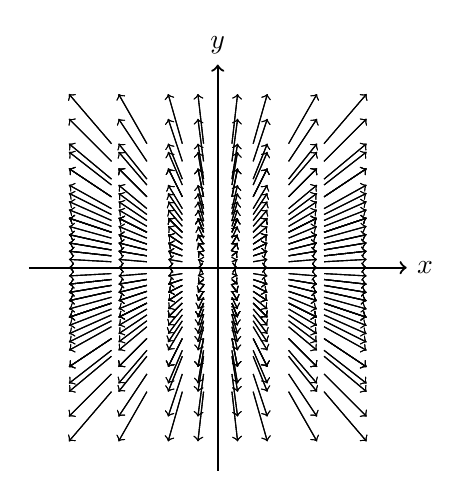
\begin{tikzpicture}[scale=0.6]
\draw[->, thick] (-4,0)--(4,0) node[right] {$x$};
\draw[->, thick] (0,-4.3)--(0,4.3) node[above] {$y$};

\def\factor{0.4}
\foreach \c in {-1.5,-1,-0.5,-0.2,0.2,0.5,1,1.5} {
\foreach \x in {-1.5,-1,-0.5,0.5,1,1.5} {
    \foreach \y [evaluate=\y as \r using int(ceil(abs(\x)+abs(\y)))] in {-1.75,-1.5,...,1.75}{
            \ifthenelse{\r=0}{}{\draw[->] (\c*1.5,\x*\y)--++(\factor*\c*1.5,\factor*\x*\y);}
    }
  }
}
\end{tikzpicture} \qquad 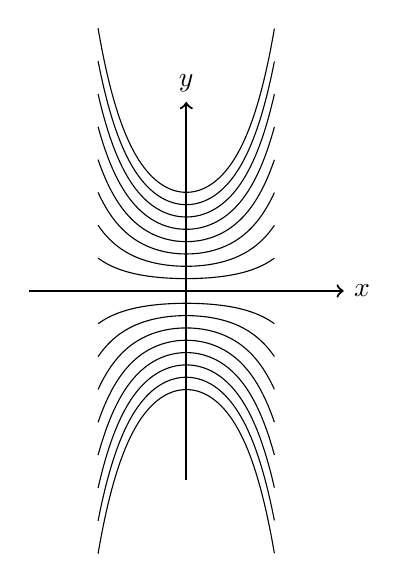
\begin{tikzpicture}[scale=0.8]
\draw[->, thick] (-2.5,0)--(2.5,0) node[right] {$x$};
\draw[->, thick] (0,-3)--(0,3) node[above] {$y$};

\foreach \xo in {-0.7,0.7} {
    \foreach \yo [evaluate=\yo as \r using int(ceil(abs(\xo)+abs(\yo)))] in {-2,-1.75,...,2}{
            \ifthenelse{\r=0}{}{\draw plot[domain=-0.7:0.7, samples=100] (\x + \xo, {\yo * exp(0.5 * \x * \x + \xo * \x)});}
    }
}
\end{tikzpicture}$$
            
Adem\'as, el dominio es todo $\mathbb R$, pues no hay puntos peculiares, $\sigma: \mathbb R \longrightarrow \mathbb R$.
\end{ejem}
\begin{ejem}
    Sea $M=(0, +\infty) \subset \mathbb R$, sea el campo $Y=\frac{1}{x} \frac{\partial}{\partial x} \in \mathfrak X(M)$, buscamos $\sigma(t)=x(t)$, $x'(t) = \frac{1}{x(t)}$, teni\'endose el sistema
    $$\begin{cases}
        x' = \frac{1}{x} \\ x(0)=x_o
    \end{cases} \Rightarrow \sigma(t) = \sqrt{2y+x_o^2}$$
    luego $\sigma: I = (-\nicefrac{1}{2} \, x_o^2, +\infty) \longrightarrow M$ es decir, el dominio de definici\'on, en general, depende de las condiciones iniciales. 
\end{ejem}

\begin{defi}
Se dice que un \textbf{campo de vectores} es \textbf{completo} si la curva integral maximal que pasa por $p$ en $t=0$ está definida para toda $t \in \mathbb{R}$.
\end{defi}
\begin{ejem}
    El que vimos en $\mathbb R^2$ es completo y el que vimos en $M=(0,\infty)$ no es completo.
\end{ejem}

\begin{prop}
Sea $M$ una variedad diferenciable y $X \in \mathfrak{X}(M)$, $p \in M$. Si $\sigma_p:(a,b)\subset \mathbb{R}\to M$ es la curva integral maximal de $X$ que en $t=0$ pasa por $p \in M$. Para todo $t_o \in [a,b]$, $q=\sigma_p(t_o)$ entonces la curva $\sigma_q(t) = \sigma_p(t + t_0)$ definida por $\sigma_q:(a-t_0,b-t_0) \to M$, es la curva integral maximal de $X$ que en $t=0$ pasa por $q = \sigma_p(t_o) \in M$.
\end{prop}
\begin{dem}
\textcolor{red}{Ejercicio}
\end{dem}

\begin{obs}
Si $(a,b)$ no estuviese acotado superior o inferiormente, tampoco lo estaría $(a-t_0,b-t_0)$.
\end{obs}

\begin{teo}
Sea $M$ una variedad diferenciable y $X \in \mathfrak{X}(M)$. Para todo $p \in M$, existe un intervalo abierto $I_p \subset \mathbb{R}$ con $0 \in I_p$, un abierto $U_p \subset M$ con $p \in U_p$ y una aplicación diferenciable $\Psi_p:I_p \times U_p \to M$ tal que:
\begin{enumerate}[a)]
    \item Para todo $q \in U_p$, la aplicaci\'on $\sigma_q(t) = \Psi_p(t,q)$ definida en $I_p$ es curva integral de $X$ con $\sigma_q(0)=q$. En particular, $\Psi_p(0,q) = q$ para todo $q \in U_p$.
    \item Si $J_p \subset \mathbb R$ y $V_p \subset M$ son abiertos y existe otra aplicación diferenciable $\Phi_p:J_p \times V_p \to M$ que cumpla las condiciones de a), entonces $$\Psi_p(t,q) = \Phi_p(t,q) \quad \forall\; (t,q) \in (I_p\cap J_p) \times (U_p \cap V_p)$$
\end{enumerate}
\end{teo}
\begin{dem}
Ver \textbf{Currás}, se demuestra aplicando la dependencia diferenciable de las soluciones de SEDO respecto a las condiciones iniciales \textcolor{red}{(gracias Ricardo por tanto)}.
\end{dem}
\begin{obs}
Los dominios de cada $\Psi_p$, $I_p \times U_p$ no quedan completamente determinados por $X$ ni $p\in M$. 
\end{obs}
\begin{obs}
Si el campo $X$ es completo, podemos tomar los $I_p = \mathbb{R} \, \forall p \in M$.
\end{obs}

\begin{defi}
A la familia $\{\Psi_p\}_{p \in M}$ de aplicaciones definidas en el teorema anterior se le llama \textbf{flujo de $X$} .
\end{defi}

\begin{teo}
Sea $M$ una variedad diferenciable y $X \in \mathfrak{X}(M)$. Para todo $t \in \mathbb{R}$, se define $D_t = \{p \in M \;/\; t$ pertenece al dominio de definición de la curva integral maximal de $X$ con condición inicial en $p\} \subset M$. Entonces:
\begin{enumerate}[a)]
    \item Para todo $t \in \mathbb{R}$, $D_t$ es abierto y $\underset{t > 0}{\bigcup} D_t = M = \underset{t < 0}{\bigcup} D_t$
    \item Si $\tau_t:D_t \subset M \to M$ es la aplicación definida por $\tau_t(p) = \sigma_p(t)$, donde $\sigma_p$ es la curva integral maximal de $X$ con condición inicial $p$, entonces $\tau_t$ es diferenciable.
    \item Para todo $t\in \mathbb{R}$, $\tau_t(D_t) = D_{-t}$
    \item $\tau_o : D_o = M \to M$ es la identidad: $\tau_o(p) = \sigma_p(0) = p$, $\tau_o=Id$.
    \item Para todos $t,s \in \mathbb{R}$, el dominio $Dom(\tau_t\circ \tau_s
    ) \subset Dom(\tau_{t+s})$ y son iguales cuando $t,s$ tienen el mismo signo. En el menor dominio se cumple que $\tau_t \circ \tau_s = \tau_{t+s}$
    \item Para todo $t \in \mathbb{R}$, $\tau_t$ es un difeomorfismo con inversa $(\tau_t)^{-1} = \tau_{-t}$.
\end{enumerate}
\end{teo}

\begin{obs} \,
\begin{itemize}
\item Si $X$ es completo, entonces $D_t = M$ para todo $t$. En tal caso, las aplicaciones $\tau_t:M\to M$ podrán componerse en todo caso, y a la familia $\{\tau_t\}_{t\in \mathbb{R}}$ se le llama \textbf{grupo uniparamétrico de transformaciones}. En efecto, la composición es una ley de grupo por las propiedades anteriores.
\item Si $X$ no es completo, algún $D_t$ depende del $t$ y en algún caso $Dom(\tau_t\circ \tau_s) \subsetneqq Dom(\tau_{t+s})$. A la familia $\{\tau_t\}_{t\in \mathbb{R}}$ se le llama \textbf{grupo uniparamétrico local de transformaciones}.
\item Si tenemos una familia de aplicaciones diferenciables $\tau_t:U_t \subset M \to M$ que verifican las propiedades a), d), e) (y en consecuencia f) ) del teorema anterior, se llama \textbf{generador infinitesimal} de la familia $\{\tau_t\}_{t \in \mathbb{R}}$ al campo de vectores
$$X_p = \sigma'_p(0) \qquad \text{donde } \sigma_p(t) = \tau_t(p) \;\forall\; p\in M, t\in \mathbb{R}$$
Se demuestra que $\sigma$ y $X$ son diferenciables, y que el grupo uniparamétrico generado por este campo es precisamente $\{\tau_t\}_{t \in \mathbb{R}}$.
\end{itemize}
\end{obs}
\begin{ejem}
    Sea $M=(a,\infty)\subset \mathbb R$ y el campo $X=\frac{1}{x} \frac{\partial}{\partial x}$, la curva integral maximla de $X$ que pasa por $x \in M$ estaba definida por
    $$\bt \sigma_x : (-\frac{1}{2}x^2, \infty) \arrow{r} & M \\[-5mm] t \arrow[mapsto]{r} & \sqrt{2t+x^2} \et$$
    Como dominio del flujo $\Psi_x$ podemos tomar $I_x=\left(-\frac{1}{4}x^2,\infty\right), \, U_x=\left(\frac{\sqrt{2}}{2}x,\infty\right)$ de modo que construimos el flujo
    $$\bt \Psi_x : I_x \times U_x \arrow{r} & M \\[-5mm] (t,y) \arrow[mapsto]{r} & \sqrt{2t+y^2} \et$$
    de forma que 
    $$D_t = \begin{cases}
        M & t \geq 0 \\ (\sqrt{-2t},+\infty) & t < 0
    \end{cases}$$
    y por tanto 
    $$\bt \tau_t : D_t \arrow{r} & M \\[-5mm] x \arrow[mapsto]{r} & \sqrt{2t+x^2} \et$$
    y queda comprobar que para $s=-1, t=2$ resulta que $Dom (\tau_t\circ \tau_s)=(\sqrt{2}, \infty) \subsetneqq M = Dom(\tau_{t+s})$ y comprobar la ley de grupo. 
\end{ejem}



 

\justifying  \setcounter{page}{52} \setcounter{chapter}{4}
\chapter{Cálculo diferencial en variedades}
\section{Campos de covectores}
\begin{defi}
Sea $M$ una variedad diferenciable y $U \subset M$ un abierto. Un \textbf{campo de covectores} en $U$ es una asignación de a cada $p \in U$ un elemento de $T_p^*M$.
\end{defi}

\begin{obs}
Como en campos de vectores, si $U = M$, el campo será global, y en otro caso se dice que es local. La notación usual para campos de covectores será $\omega$ o $\theta$, y la evaluación en $p\in U$ se escribirá $\omega_p,\theta_p \in T_p^*M$.
\end{obs}

Si $\omega$ es un campo de covectores en $U \subset M$ y $(V,\varphi\equiv(x_i))$ es una carta de $M$ sabemos que $\{d_px_i\}_{i=1}^n$ es base de $T_p^*M$. Entonces, para todo $p \in U \cap V$ se tiene que $$\omega_p =  \sum_{i=1}^n \lambda_i(p) d_px_i \qquad \text{con } \lambda_i: U\cap V \to \mathbb{R}$$

\begin{defi}
Sea $M$ una variedad diferenciable y un \textbf{campo de covectores} en el abierto $U \subset M$. Se dice que $\omega$ es \textbf{diferenciable} si para todo $p \in U$ existe una carta $(V,\varphi)$ de $M$ con $p \in V$ de modo que las funciones coordenada de $\omega|_{U\cap V}$ en la base que genera $(V,\varphi)$ son diferenciables. Al conjunto de campos de covectores diferenciables en $U$ lo denotaremos por $\Lambda_1(U)$.
\end{defi}

\begin{obs} \, \vspace{-3mm} \begin{enumerate}[a)] \item Si la condici\'on de diferenciabilidad se cumple para $(V,\psi)$ con $p\in V$, se cumplir\'a para c
ualquier otra carta que cubra a $p$. 
\item En algunos textos se denota por $\Omega_1(U)$ en lugar de $\Lambda_1(U)$. \item A los campos de covectores diferenciables tambi\'en pueden ser llamados campos de 1-formas.
\end{enumerate}
\end{obs}

\begin{ejem} \,
\begin{enumerate}
    \item Si $(U,\varphi\equiv(x_i))$ es una carta de $M$, $\pd{}{x_i} \in \mathfrak X (U), \, dx_i \in \Lambda_1(U)$.
    \item Si $f\in \mathcal C^{\infty}(U), \, U\subset M$ abierto, entonces $df \in \Lambda_1(U)$. 
    \item Si $(U,\varphi\equiv(x_i))$ es carta de $M$,  entonces $dx_i \in  \Lambda_1(U)$, pues dado $p \in U$ este campo valora como $(dx_i)_p = d_px_i \in T_p^*M$. 
    
    También, si $f\in \mathcal{C}^{\infty}(V)$, se tiene que $df\in \Lambda_1(V)$, pues para todo $p \in V$ se valora como $(df)_p = d_pf \in T_p^*M$ y $$df|_{U\cap V} = \sum_{i=1}^n \dfrac{\partial}{\partial x_i}(f) dx_i|_{U\cap V}$$
\end{enumerate}

\end{ejem}

\begin{prop}
Si $U\subset M$ es un abierto de una variedad diferenciable $M$, entonces $\Lambda_1(U)$ es un $\mathcal{C}^{\infty}(U)$-módulo con las operaciones definidas para todo $p\in U$:
\begin{itemize}
    \item $(\omega+\theta)_p = \omega_p + \theta_p \in T_p^*M \qquad \forall\;\omega,\theta \in \Lambda_1(U)$
    \item $(\lambda\omega)_p=\lambda \cdot \omega_p \in T_p^*M \qquad \qquad \forall \; \omega\in \Lambda_1(U), \, \lambda \in \mathbb R^*$ 
    \item $(f\,\omega)_p = f(p)\cdot \omega_p \in T_p^*M \qquad \forall\; \omega\in \Lambda_1(U), f\in\mathcal{C}^{\infty}(U)$
\end{itemize}
\end{prop}
\begin{dem}
\textcolor{red}{Ejercicio, no lo va a hacer ni dios}
\end{dem}

Si $\omega$ es un campo de covectores en $U$, entonces para todo $p \in U$ las formas $\omega_p$ actúan sobre elementos de $T_pM$, que a su vez pueden venir de un campo de vectores $X$ sobre $U$. Esta actuación es de la forma $$\begin{tikzcd}
\omega(X):\hspace{-13mm} & U \rar & \mathbb{R}\\[-5mm]
& p \arrow[rightsquigarrow]{r} & \omega_p(X_p)
\end{tikzcd}$$

\begin{prop}
Sea $\omega$ un campo de vectores en un abierto $U \subset M$ de una variedad diferenciable. Entonces 
$$\omega \in \Lambda_1(U) \iff \;\forall\; X \in \mathfrak{X}(U),\;\; \omega(X) \in \mathcal{C}^{\infty}(U)$$
\end{prop}
\begin{dem}
\textcolor{red}{Ejercicio sencillo, parecido al de vectores}
\end{dem}
\begin{obs}
Si $Y$ es otro campo de vectores en $U$ y $X_p = Y_p$, entonces $\omega(X)(p) = \omega(Y)(p)$ para todo $\omega \in \Lambda_1(U)$. Esto no suced\'ia con campo de vectores, pues que $(Xf)$ y $(Xg)$ coinciden en $p$, \underline{no} implica que $(Xf)=(Xg)$ pues la derivada es local, no puntual.
\end{obs}

\begin{defi}
Sean $M,N$ variedades diferenciables, $f:M\to N$ una aplicación diferenciable y $\omega$ un campo de covectores en $N$. Se llama \textbf{pull-back} o \textbf{retroacción de} $\omega$, y se denota por $f^*\omega$, al campo de covectores de $M$ dado por 
$$\forall\; p \in M \qquad (f^*\omega)_p = f^*_p(\omega_{f(p)}) \in T_p^*M$$
donde $f_{,p}^*: T_{f(p)}^*N \longrightarrow T_p^*M$ es la aplicaci\'on cotangente de $f$ en $p\in M$.
\end{defi}
\begin{obs}
    Si $\omega$ est\'a definido en $V \subset N$ abierto, entonces $f^*\omega$ estar\'a definido en $f^{-1}(V)$.
\end{obs}
\begin{prop}
Si $f:M\to N$ es diferenciable y $\omega\in \Lambda_1(N)$, entonces $f^*\omega \in \Lambda_1(M)$.
\end{prop}
\begin{dem}
\textcolor{red}{Ejercicio.} Usar que dada la carta de $N$: $(V,\psi\equiv(y_j))$, entonces si $\displaystyle \omega|_V=\sum_{i=1}^n \lambda_i dy_j$, $\forall p \in f^{-1}(V)$
\[ \begin{split}(f^*\omega)_p & =f_p^*(\omega_{f(p)})=f^*(\omega|_V)= f^*(\sum \lambda_i(f(p)) d_{f(p)}y_j) = \sum \lambda_i(f(p)) f^*_p (d_{f(p)}y_j) = \\ & =\sum(\lambda_i \circ f)(p) d_p(y_i \circ f) \end{split} \]
y si $(U,\varphi\equiv(x_i))$ es carta de $M$, $f(U)\subset V$, las coordenadas de $f^*_p\omega$ en esta base, viene determinada por 
$$d_p(y_i\circ f) \left( \pd{}{x_i}\Big|_p \right)= \pd{}{x_j}\Big|_p(y_i\circ f)$$
y as\'i comprobamos que es diferenciable.
\end{dem}

\begin{obs}
\textcolor{blue}{Comprobar si la asignación $M \to \Lambda_1(M)$, $f \to f^*$ es funtorial.}
\end{obs}

\section{Campos de tensores} \footnote{En el examen final entra todo sobre campos de tensores, no el recordatorio de tensores en espacios vectoriales. Las demostraciones de los dos \'ultimos apartados no se pedir\'an debido a su complejidad y longitud (las de campos de tensores s\'i). Sin embargo, s\'i se pedir\'an definiciones y manejo de las derivadas de Lie y diferencial exterior}
Lo estudiado en esta secci\'on se encuentra en los ap\'endices que se enlazan a continuaci\'on

\hyperref[ap1]{Tensores. Espacios vectoriales.}

\hyperref[ap2]{Campos de tensores}

\hyperref[ap3]{Derivada de Lie}

\hyperref[ap4]{Diferencial exterior}
\begin{defi}
    Sea $M$ una variedad diferenciable y $T\in \mc T_s^r(M)$, sea $k \in \{1,\ldots, r\}, \, l\in \{1,\ldots, s\}$. Se llama \textbf{contracci\'on tensorial} del $k$-\'esimo \'indice contravariante y $l$-\'esimo \'indice covariante de $T$ al campo tensorial:
    $$(C_l^kT)_p=C_l^k(T_p) \in T_{s-1}^r(T_pM) \qquad \forall \, p \in M$$
    se define la contracci\'on en $T_pM$, $C_l^k$ en \hyperref[ap2]{Campos de tensores}.
\end{defi}
\begin{defi}
    Si $T \in \mc T_s(M)$ y $X\in \mathfrak{X}(M)$, se llama \textbf{producto interior} de $T$ por $X$, o producto contra\'ido de $T$ por $X$, al campo tensorial $i_XT\in \mc T_{s-1}(M)$ dado por:
    $$(i_XT)(Y_1, \ldots, Y_{s-1})=T(X,Y_1, \ldots, Y_{s-1})$$
\end{defi}
\begin{ejem}
    Consideremos en $\mathbb R^3$ con las coordenadas usuales, el tensor
    $$T = x\left(dx\otimes dy\otimes \pd{}{z}\right)  + (xyz)  \left(dy\otimes dx \otimes \pd{}{x}\right) \in \mc T_2^1(\mathbb R^3)$$
    entonces
    \[ \begin{split} C_1^1T & =xC_1^1\left(dx\otimes dy\otimes \pd{}{z}\right) + xyzC_1^1 \left(dy\otimes dx \otimes \pd{}{x}\right)=x\cancelto{0}{dx \left( \pd{}{z} \right)}dy + xyz \cancelto{0}{dy\left(\pd{}{x}\right)}dx = \\ & = 0\end{split}\]
    \[\begin{split} C_2^1T & =xC_2^1\left(dx\otimes dy\otimes \pd{}{z}\right) + xyzC_2^1 \left(dy\otimes dx \otimes \pd{}{x}\right)=x\cancelto{0}{dy \left( \pd{}{z} \right)}dx + xyz \cancelto{1}{dx\left(\pd{}{x}\right)}dy= \\ & = xyz \, dy\end{split}\]
\end{ejem}
\begin{ejem}
    Sea el tensor
    $$T=(1+z)dx \otimes dy + xy \, dy \otimes dy + (x+z) dy \otimes dz \in \mc T_2(\mathbb R^3)$$
    y el campo
    $$X=2\pd{}{x}+x\pd{}{y} \in \mathfrak X(\mathbb R^3)$$
    entonces
    \[\begin{split}
        (i_X \Tilde{X}) & = (1+z)i_X(dx\otimes dy) + xy i_X(dy\otimes dy) + (z+x)i_X(dy\otimes dz) = \\ &= (1+z) \cdot dx(X) \cdot dy + xy dy(X) dy + (x+z) dy(X) dz = \\ & = (1+z) \, 2 \, dy + xy \cdot x \, dy +(x+z) \cdot 1 \cdot dz = \\& = 
        (2(1+z)+x^2y)dy+(x+z)dz \in \mc T_1^0(\mathbb R^3) = \Lambda_1(\mathbb R^3)
    \end{split}\]
\end{ejem}

\begin{defi}
    Sea $M$ una variedad diferenciable y sea $X \in \mathfrak X(U)$ un campo. La \textbf{derivaci\'on de Lie} en la direcci\'on $X$ es un operador $L_X: \mc T_s^r(M) \longrightarrow \mc T_s^r(M)$ $\mathbb R$-lineal.
\end{defi}
Obs\'ervense los siguientes casos:\vspace{-3mm}
\begin{enumerate}
    \item Si $r=s=0$, $f\in \mc T_0^0(M) = \mc C^{\infty}(M)$, entonces
    $$L_Xf=X\,f\in \mc C^{\infty}(M)$$
    \item Si $Y \in \mathfrak X(M)=\mc T_0^1(M)$ entonces
    $$L_XY=[X,Y] \in \mathfrak X(M)$$
    \item Si $\omega \in \Lambda_1(M) =\mc T_1^0(M)$ entonces
    $$(L_X\omega)(Y)=X(\omega(Y))-\omega(L_XY) = X(\omega(Y))-\omega[X,Y]\qquad \forall \, Y \in \mathfrak X(M)$$
    \item Si $T\in \mc T_s^r(M)$, entonces
    \[\begin{split}
        (L_XT)&(\underbrace{x_1,\ldots,x_s}_{\mathfrak X(M)},\underbrace{\omega_1,\ldots,\omega_r}_{\Lambda_1(M)}) = X\big(T(x_1,\ldots,x_s,\omega_1,\ldots,\omega_r)\big) - \\ & -\sum_{k=1}^s T(x_1,\ldots,L_Xx_i, \ldots, x_s,\omega_1,\ldots,\omega_r) - \\ & - \sum_{j=1}^r T(x_1,\ldots,x_s,\omega_1,\ldots,L_X\omega_j, \ldots, \omega_r)
    \end{split}\]
    que se trata de una definici\'on axiom\'atica, en la que hay que comprobar que est\'a bien definido y se verifica $\mathbb R$-linealidad y diferenciabilidad. 
\end{enumerate}
\begin{propis}
    Se verifican las siguientes propiedades \vspace{-3mm}
    \begin{itemize}
        \item $L_{\lambda X+\mu Y}=\lambda L_X+\mu L_Y$
        \item $L$ deriva $\otimes$: $L_X(T\otimes \overline{T})= L_X T \otimes \overline{T} + T \otimes L_X \overline{T}$
        \item $\omega \in \Lambda_s(M)\Rightarrow L_X\omega \in \Lambda_s(M)$. En particular,
        \item $L$ deriva $\wedge$: $L_X(\omega_1\wedge \omega_2)=L_X\omega_1\wedge \omega_2 + \omega_1 \wedge L_X\omega_2$.
        \item $f\in \mc C^{\infty}(M)$, $L_X(df)=d(Xf)=d(L_Xf)$
    \end{itemize}
\end{propis}
\begin{ejem}
    En $\mathbb R^2$, dado el campo 
    $$X=y \pd{}{x}-\pd{}{y} \in \mathfrak(\mathbb R^2)$$
    y los tensores
    $$T=xydx+(1-x)dy \in \Lambda_1(\mathbb R^2) \qquad \overline{T}=dx\otimes \pd{}{y} + (x^2+y^2)dy \otimes \pd{}{x} \in \mc T_1^1(\mathbb R^2)$$
    entonces
    $$L_X(dx)=d(X_x)=d(y)=dy \qquad L_X(dy)=d(Xy)=d(-1)=0$$
    $$L_X\left(\pd{}{x}\right) = \left[X,\pd{}{x}\right] = \left[y\pd{}{x}-\pd{}{y},\pd{}{x}\right] = 0 $$
    $$L_X\left(\pd{}{y}\right)=\left[X,\pd{}{y}\right]=\left[y\pd{}{x}-\pd{}{y},\pd{}{y}\right]=\pd{}{x}$$de forma que
    \[\begin{split} L_XT & =L_X(xy \, dx) + L_X((1-x)dy)=L_X(xy\otimes dx)+ L_X((1-x)\otimes dy) = \\ & = L_X(xy)\otimes dx + xy \otimes L_Xdx + L_X(1-x) \otimes dy + (1-x)\otimes L_X dy = \\ & = (y^2-x) \otimes dx + xy \otimes dy - y\otimes dy =(y^2-x) dx + (xy-y) dy \end{split}\]
    \[\begin{split}
        L_X\overline{T} & = L_X\left(dx\otimes \pd{}{y} \right) + L_X\left(x^2+y^2\otimes dy \otimes \pd{}{x}\right) = \cdots = \hspace{28mm} \\ & = dy \otimes \pd{}{y}+2xy-2y dy\otimes \pd{}{x}-dx\otimes \pd{}{x}
    \end{split}\]
\end{ejem}\begin{teo}
    Sea $M$ una variedad diferenciable, entonces existe un \'unico operador \\ $d:\bigwedge_s(M) \longrightarrow \bigwedge_{s+1}(M)$ $\mathbb R$-lineal que cumple: \vspace{-3mm}
    \begin{enumerate}
        \item Para $s=0$, $\bigwedge_o(M) = \mc C^{\infty}(M)$ es la diferencial de funciones ya conocida ($f\longmapsto df$)
        \item $d^2=d\circ d=0$
        \item Es una antiderivaci\'on de grado 1, es decir, $\forall \omega \in \Lambda_r(M), \theta \in \Lambda_s(M)$,
        $$d(\omega \wedge \theta)=d\omega \wedge \theta + (-1)^r \omega \wedge d\theta$$
    \end{enumerate}
\end{teo}
\begin{obs}
    De la (no) demostraci\'on, se ve que si
    $$\omega|_M = \sum_{1\leq i_1 < \cdots < i_r \leq n} \lambda_{i_1,\ldots,i_r} dx_{i_1}\wedge \cdots \wedge dx_{i_r}$$
    entonces
    $$d\omega|_M = \sum_{1\leq i_1 < \cdots < i_r \leq n} d(\lambda_{i_1,\ldots,i_r}) \wedge dx_{i_1}\wedge \cdots \wedge dx_{i_r}$$
\end{obs}

\section{Conexiones lineales}

\begin{defi}
Sea $M$ una variedad diferenciable. Una conexión lineal es un operador $\nabla:\mathfrak{X}(M) \times \mathfrak{X}(M) \longrightarrow \mathfrak X(M)$ que cumple:
\begin{enumerate}
    \item Es $\mathbb{R}$-lineal en ambos componentes: $\forall \;X, Y,Z \in \mathfrak{X}(M),\lambda \in \mathbb{R}$ $$\nabla_{(X + \lambda\,Y)}Z = \nabla_X X + \lambda\,\nabla_Y Z \qquad \nabla_X(Y + \lambda\,Z) = \nabla_X\,Y + \lambda\,\nabla_X\,Z$$
    \item Es $\mathcal{C}^{\infty}$-lineal en la primera componente, es decir, para toda $f\in \mathcal{C}^{\infty}$ $$\nabla_{fX}Y = f \,\nabla_X\,Y$$
    \item Es una derivación en la segunda componente: $$\nabla_X(fY) = (Xf)\cdot Y + f\nabla_X\,Y$$
\end{enumerate}
\end{defi}

\begin{ejem}
En $\mathbb{R}^n$ con las coordenadas usuales $\{x_1,\dots,x_n\}$, sean $X,Y \in \mathfrak{X}(\mathbb{R}^n)$, con $\displaystyle Y = \sum_{i=1}^n \lambda_i \dfrac{\partial}{\partial x_i}$, se define
$$\nabla_X\,Y = \sum_{i=1}^n X(\lambda_i)\dfrac{\partial}{\partial x_i} \in \mathfrak{X}(\mathbb{R}^n)$$
Es directo comprobar que se cumplen las condiciones de la definición. Se llamará a esta aplicación conexión usual de $\mathbb{R}^n$.
\end{ejem}

\begin{ejem}
El corchete de Lie \textbf{no} es una conexión lineal, pues no es $\mathcal{C}^{\infty}$-lineal en la primera componente.
\end{ejem}

\begin{teo}
Sea $M$ una variedad diferenciable y $\nabla$ una conexión. Sean $X_1,X_2,Y_1,Y_2 \in \mathfrak{X}(M)$ de modo que para cierto $p \in M$, $(X_1)_p = (X_2)_p$ y existe $U \subset M$ abierto con $p \in U$ tal que $Y_1|_U = Y_2|_U$. Entonces $$(\nabla_{X_1}\,Y_1)_p = (\nabla_{X_2}\,Y_2)_p$$
\end{teo}
\begin{dem}
Por la $\mathbb{R}$-linealidad, basta probar que si $X_p = 0$ entonces $(\nabla_X\,Y)_p = 0$ y que si $Y|_U = 0$ entonces $(\nabla_X\,Y)_p = 0$.

Veamos que si existe $U \subset M$ abierto con $p \in U$ y $Y|_U = 0$, entonces $(\nabla_X\,Y)_p = 0$. Para $p \in U$, escogeremos una función meseta $h:M\to [0,1]$ diferenciable, de soporte compacto y contenido en $U$, con lo que existe un abierto $V$ con $p \in V \subset \overline{V} \subset U$ tal que $h|_{\overline{V}} \equiv 1$. Generamos $\overline{h} = 1-h$, diferenciable y con $\overline{h}|_{\overline{V}} \equiv 0, \overline{h}|_{M-U} \equiv 1$. Se cumple por tanto que $Y = \overline{h} Y$, pues en $U$ $Y\equiv 0$, y fuera la función meseta es la identidad. Luego
$$(\nabla_X\,Y)_p = (\nabla_X(\overline{h}Y))_p = ((X\overline{h})\cdot Y + \overline{h}\,\nabla_X Y)_p = (X\overline{h})(p) \cdot Y_p + \overline{h}(p)\cdot (\nabla_X Y) = 0$$
Análogamente se demuestra que $X = \overline{h}\,X$, con lo que 
$$(\nabla_X\,Y)_p = (\nabla_{\overline{h}X} Y)_p = (\overline{h}\cdot\nabla_X Y)_p = \overline{h}(p)(\nabla_X Y)_p = 0$$
Así que si $X|_U \equiv 0$ entonces $\nabla_X Y|_U \equiv 0$.

Veamos ahora que si $X_p = 0$, entonces $(\nabla_X Y)_p = 0$. Sea $(V,\varphi\equiv (x_i))$ una carta de $M$ con $p \in V$. Podemos expresar
$$X|_V = \sum_{i=1}^n \lambda_i \dfrac{\partial}{\partial x_i} \in \mathfrak{X}(V)$$
y ya que $X_p = 0, \lambda_i(p) = 0$ para todo $i$. Sea $h:M \to [0,1]$ una función meseta asociada a $p\in V$ diferenciable de soporte compacto y contenido en $V$, y existiendo $\omega \subset V$ abierto con $p \in \omega \subset \overline{\omega} \subset V$ tal que $h|_{\overline{\omega}} \equiv 1$.
Extendemos $\lambda_i$ a una función global y $\dfrac{\partial}{\partial x_i}$ a campos globales.
$$\mu_i = \begin{cases}
h\cdot \lambda_i \quad \text{en } U\\
0 \qquad \text{en } M-sop(h)
\end{cases} \qquad Z_i = \begin{cases}
h \cdot \dfrac{\partial}{\partial x_i}  \quad \text{en } U\\
0 \qquad \text{en } M-sop(h)
\end{cases}$$
Con lo que las $\mu_i$ son funciones globales y $Z_i$ son campos globales, verificando que $$Z = \sum_{i=1}^n \mu_i \,Z_i \in \mathfrak{X}(M) \qquad Z|_\omega = \sum_{i=1}^n \lambda_i \,\dfrac{\partial}{\partial x_i}\Big|_\omega = X|_\omega$$
con lo que $$(\nabla_X Y)_p = (\nabla_Z Y)_p = \left(\sum_{i=1}^n \mu_i \;\nabla_{Z_i} Y\right)_p = \sum_{i=1}^n \mu_i(p) (\nabla_{Z_i} Y)_p = 0$$
ya que $\mu_i(p) = \lambda_i(p) = 0$.
\end{dem}
\begin{notc}
    Como $(\nabla_XY)_p$ depende de $X_p$ y $Y|_U$ donde $U\subset M$ abierto, tiene sentido la notaci\'on, para $p\in M$, $v\in T_pM$, $Y \in \mathfrak X(U)$, $U$ abierto con $p\in U$
    $$\nabla_vY=(\nabla_X Y)_p$$
    para cualquier campo diferenciable $X$ con $X_p=v$.
\end{notc}

\begin{teo}
    Sea $M$ una variedad diferenciable, $\nabla$ una conexión, $p \in M$, $\sigma: I \subset \mathbb{R} \to M$ una curva diferenciable con $\sigma(0) = p$ y $\sigma'(0)=v \in T_pM$. Si $Y,Z \in \mathfrak X(M)$ son tales que $Y_{\sigma(t)} = Z_{\sigma(t)}$ para todo $t \in I$, entonces $$\nabla_v Y = \nabla_v Z$$
\end{teo}
\begin{dem}
    Por la linealidad de $\nabla$ basta probar que si $Y_{\sigma(t)} = 0$ para todo $t \in I$, entonces $\nabla_v Y = 0$.
    Para $p = \sigma(0)$, consideramos una carta $(U,\varphi\equiv (x_i))$ de $M$ con $p\in U$. Entonces $Y|_U = \sum_{i=1}^n \lambda_i \dfrac{\partial}{\partial x_i}$ con $\lambda_i \in \mathcal{C}^{\infty}(U)$ de modo que $\lambda_i(\sigma(t)) = 0$ para todo $t \in \sigma^{-1}(U) \subset I$. Conocemos $\sigma(t)$, es decir, $\varphi \circ \sigma(t) = (x_1(t),\dots,x_n(t))$ y $\sigma'(t) \in T_{\sigma(t)}M$. Por tanto
    \[ \begin{split}\nabla_v Y & = (\nabla_{\sigma'(t)} Y)_{t=0} = \nabla_{\sigma'(t)}\left(\sum_{i} \lambda_i \dfrac{\partial}{\partial x_i} \right)\Big|_{t=0}= \\ & =\sum_{i=1}^n \left( \sigma'(0)(\lambda_i) \dfrac{\partial}{\partial x_i}\Big|_p + \lambda_i(\sigma(0)) \nabla_{\sigma'(0)}\dfrac{\partial}{ \partial x_i} \right) = \sum_{i=1}^n \dfrac{\partial (\lambda_i \circ \sigma)}{\partial t}\Big|_{t=0} \dfrac{\partial}{\partial x_i}\Big|_p = 0 \end{split} \] 
    \hfill $\blacksquare.$
\end{dem}

Esto recuerda a la definición de campo tangente, o con soporte, a lo largo de una curva. Si $\sigma: I \subset \mathbb{R} \to M$  es una curva diferenciable, denotaremos por $\mathfrak X(\sigma)$ al conjunto de campos diferenciables definidos a lo largo de $\sigma$. Esto es, si $X \in \mathfrak X(\sigma)$, entonces $X(t) \equiv X_{\sigma(t)} \in T_{\sigma(t)}M$ de modo que al escribir $X$ en coordenadas locales $(U, \varphi\equiv (x_i))$ como $\displaystyle X(t) = \sum_{i=1}^n \lambda_i(t) \dfrac{\partial}{\partial x_i}\Big|_{\sigma(t)}$ se tiene que $\lambda_i \in \mathcal{C}^{\infty}(I\cap \sigma^{-1}(U))$.
\begin{ejem}
    Dada $\sigma: I \subset \mathbb R \to M$ diferenciable, el campo $\sigma'(t) \in \mathfrak X(\sigma)$ se llama campo de velocidades de $\sigma$.
\end{ejem}
\begin{prop}
    El conjunto $\mathfrak X(\sigma)$ es un $\mathcal{C}^{\infty}(I)$-módulo, es decir, que si $f: I \subset \mathbb R \longrightarrow \mathbb R$, $X\in \mathfrak X(U)$ podemos definir $f\cdot X \in \mathfrak X(U)$.
\end{prop}
\begin{dem}
    \textcolor{red}{Ejercicio}
\end{dem}

\begin{prop}
    Sea $M$ una variedad diferenciable, $\nabla$ una conexión y $\sigma: I\subset \mathbb R \to M$ una curva diferenciable. El operador derivada covariante a lo largo de $\sigma$ $$\begin{tikzcd}
    \nabla_{\sigma'}: \hspace{-10mm} & \mathfrak X(\sigma) \rar & \mathfrak X(\sigma)\\[-5mm]
    & X \arrow[mapsto]{r} & \nabla_{\sigma'} X
    \end{tikzcd}$$ está bien definido y es $\mathbb R$-lineal, donde $(\nabla_{\sigma'} X)(t) = \nabla_{\sigma'(t)} X \in T_{\sigma(t)}M$. Además, para todo $f \in \mathcal{C}^{\infty}(I)$ se cumple que $$\nabla_{\sigma'}(fX) = f' X + f\nabla_{\sigma'} X$$
\end{prop}
\begin{dem}
    \textcolor{red}{Ejercicio}
\end{dem}
\begin{obs}
    La notación clásica en teoría de superficies es $\dfrac{D}{dt}$, que no incluye a la curva $\sigma$.
\end{obs}


\begin{defi}
    Sea $M$ una variedad diferenciable, $\nabla$ una conexión y $(U,\varphi\equiv (x_i))$ una carta de $M$. Se llaman \textbf{coeficientes de la conexión en la carta} $(U,\varphi)$ a las $n^3$ funciones diferenciables $\left\{\Gamma_{ij}^k\right\}_{i,j,k=2}^n$ dadas por $$\nabla_{\frac{\partial}{\partial x_i}} \dfrac{\partial}{\partial x_j} = \sum_{k =1}^n \Gamma_{ij}^k \dfrac{\partial}{\partial x_k}$$
\end{defi}
\begin{obs}
    Estos coeficientes son funciones de $\mathcal{C}^{\infty}(U)$.
\end{obs}
\begin{obs}
    En algunos textos, se denominan símbolos de Christoffel.
\end{obs}
\begin{ejem}
    La conexión usual de $\mathbb R^n$ en las coordenadas usuales, siendo $X, Y \in \mathfrak X(\mathbb R^n)$ con $\displaystyle Y=\sum_{i=1}^n \lambda_i \pd{}{x_i}$
    $$\nabla_X Y = \sum_i X(\lambda_i) \pd{}{x_i}$$
    tiene todos sus coeficientes nulos, es decir, $\Gamma_{ij}^k = 0 \, \forall \, i,j,k$. Tal vez no sean nulos en otras coordenadas.
\end{ejem}

\begin{prop}
    Sea $M^m$ una variedad diferenciable, $\nabla$ una conexión y $\{\Gamma_{ij}^k\}_{i,j,k=1}^n, \{\overline{\Gamma}_{\alpha \beta}^{\gamma}\}_{\alpha,\beta,\gamma = 1}^n$ son los coeficientes de la conexión en las cartas $(U,\varphi\equiv (x_i))$ y $(V,\psi\equiv (\overline{x}_i))$, respectivamente, entonces en $U \cap V$ se cumple
    $$\overline{\Gamma}_{\alpha \beta}^{\gamma} = \sum_{i,j,k=1}^n \Gamma_{ij}^k \dfrac{\partial x_i}{\partial \overline{x}_{\alpha}} \dfrac{\partial x_j}{\partial \overline{x}_{\beta}} \dfrac{\partial \overline x_{\gamma}}{\partial x_k} + \sum_{i=1}^n \dfrac{\partial^2 x_i}{\partial \overline x_{\alpha} \partial \overline x_{\beta}} \dfrac{\overline x_{\gamma}}{\partial x_i} \qquad \forall \alpha,\beta,\gamma \in  \{1,\dots,n\}$$
\end{prop}
\begin{dem} \textcolor{red}{Ejercicio} \\ Idea:
$$\nabla_{\frac{\partial}{\partial \overline{x}_{\alpha}}} \pd{}{\overline{x}_{\beta}} = \sum_{\alpha,\beta,\gamma} \overline{\Gamma}_{\alpha\beta}^{\gamma} \pd{}{\overline{x}_{\gamma}}$$
pudiendo realizar un cambio de coordenadas a $\pd{}{x_i}$ y teni\'endose la f\'ormula.
\end{dem}


\begin{defi}
    Sea $M$ una variedad diferenciable, $\nabla$ una conexión y $\sigma: I \subset \mathbb R \to M$ una curva diferenciable. Dado un \textbf{campo} $X \in \mathfrak X(\sigma)$, se dice que es \textbf{paralelo} a lo largo de $\sigma$ si $\nabla_{\sigma'(t)} X = 0 \, \forall\, t \in I$.
\end{defi}

\begin{obs}
    Por tanto, los campos paralelos ``no varían'' al recorrer $\sigma$.
\end{obs}

\begin{teo}
    Sea $M$ una variedad diferenciable, $\nabla$ una conexión y $\sigma: I \subset \mathbb R \to M$ una curva diferenciable con $0 \in I, p = \sigma(0) \in M$ y $v\in T_pM$. Existe un único $X \in \mathfrak X(\sigma)$ que es paralelo a lo largo de $\sigma$ verificando que $X(0) = X_p = v$.
\end{teo}
\begin{dem}
    Para el $p = \sigma(0) \in M$ del enunciado, sea $(U,\varphi\equiv (x_i))$ una carta de $M$ con $p \in U$ y sean $\{\Gamma_{ij}^k\}_{i,j,k=1}^n$ los coeficientes de la conexi\'on y $\left\{ \pd{}{x_i}\big|_q\right\}_{i=1}^n$ una base de $T_qM \, \forall \, \in U$. En particular,
    $$v = \sum_{i=1}^n v_i \pd{}{x_i}\Big|_p \in T_pM$$
    y por tanto
    $$\sigma'(t) = \sum_{i=1}^n \lambda_i(t) \dfrac{\partial}{\partial x_i}\Big|_{\sigma(t)} \in T_{\sigma(t)}M$$    
    con $\lambda_i \in \mathcal{C}^{\infty}(I)$ funciones conocidas.
    
    Supongamos que $\sigma(I) \subset U$, es decir, que la traza de la curva está contenida en este abierto coordenado.
    
    Buscamos $$X_{\sigma(t)} = \sum_{i=1}^n \mu_i(t)  \dfrac{\partial}{\partial x_i}\Big|_{\sigma(t)}$$
    que sea diferenciable y paralelo a lo largo de $\sigma$, es decir, con $\mu_i$ diferenciables, $\mu_i(0) = v_i$ para todo $i = 1,\dots,n$ y $\nabla_{\sigma'} X = 0$.

    Eliminando de la notación la variable $t$ cuando no se produzca confusión, tenemos: \[ \begin{split} \nabla_{\sigma'} X & = \nabla_{\sigma'}\left(\sum_{i=1}^n \mu_i \dfrac{\partial}{\partial x_i}\right) = \sum_{i=1}^n\left(\sigma'(t)(\mu_i) \dfrac{\partial}{\partial x_i} + \mu_i \nabla_{\sigma'}\dfrac{\partial}{\partial x_i}\right) = \\ & = \sum_{i=1}^n \mu'_i \dfrac{\partial}{\partial x_i} + \sum_{i,j=1}^n\mu_i \lambda_j \nabla_{\frac{\partial}{\partial x_j}} \dfrac{\partial}{\partial x_i}  = \sum_{i=1}^n \mu'_i \dfrac{\partial}{\partial x_i} + \sum_{i,j=1}^n \mu_i \lambda_j \left( \sum_k (\Gamma_{ji}^k \circ \sigma) \cdot \dfrac{\partial}{\partial x_k}\right) = \\ & = \sum_{k=1}^n \left(\mu'_k + \sum_{i,j} \mu_i \lambda_j (\Gamma_{ji}^k \circ \sigma) \right) \dfrac{\partial}{\partial x_k}\end{split}\]
    Junto con la condici\'on inicial $X_{\sigma(0)} = v$, $X$ ser\'a paralelo a lo largo de $\sigma$ si y solo si
    $$\begin{cases}
        \displaystyle \mu'_k + \sum_{i,j} \mu_i \lambda_j (\Gamma_{ji}^k \circ \sigma) = 0 \\ \mu_k(0)=v_k
    \end{cases} \qquad \forall \, k =1, \ldots, n$$

    Tenemos un sistema de ecuaciones diferenciales ordinarias de primer orden. Por el teorema de existencia y unicidad, sabemos que existen $\mu_1(t),ldots, \mu_n(t)$ y son únicas. Además, por ser lineal, la solución está definida para todo $t \in I$. Con esto queda probado el teorema en el caso $\sigma(I) \subset U$.

    Si no hay una carta $(U, \varphi)$ tal que $\sigma(I)\subset U$ procederemos de la siguiente manera: dado $t \in I, t>0$, vamos a definir $X$ en $[0,t]$ para que sea paralelo a lo largo de $\sigma$. Para distintos $t_1,t_2> 0 $, la unicidad del sistema de ecuaciones proporcionaría un único campo en la intersecci\'on de los dominios. An\'alogamente $\forall t< 0$ en $[t,0]$. Tendremoas as\'i definido $X \in \mathfrak X$ que sea paralelo a lo largo de $\sigma \, \forall \, t \in I$. 
    
    Como $[0,t]$ es compacto, se tiene que $\sigma([0,t])$ es compacto y existirá una cantidad finita de cartas $(U_i,\varphi_i)$ con $i=1,\ldots, m$ tal que  $\sigma([0,t]) \subset \bigcup U_i$. Si $\sigma^{-1}(U_k)$ no es conexo, tomando las distintas componentes conexas, conseguimos que $\sigma([0,t])$ est\'a recubierto por una cantidad finita de conexos.

    Aplicamos el procedimiento anterior para cada una de estas cartas. Es decir, $\exists \, U_{i_o} \, / \, p \in U_{i_o}$ con $\sigma^{-1}(U_{i_o})\subset I$, y obtenemos soluci\'on. Existir\'a entonces $\sigma(t_1)\subset U_{i_o} \cap U_{i_1}$ y buscamos soluci\'on en $\sigma^{-1}(U_{i_1})$ con la misma condici\'on inicial $X_{\sigma(t_1)}$. La unicidad de la resoluci\'on de las ecuaciones diferenciales me propoeciona un \'unico campo en el dominio intersecci\'on. Así, procederemos recursivamente. El procedimiento tiene fin, pues hay una cantidad finita de estos abiertos. Este argumento final es más detallado de lo que parece, pero no lo abordamos en esta demostración.
\end{dem}

\begin{defi}
    Sea $M$ una variedad diferenciable, $\nabla$ una conexión y $\sigma: I \subset \mathbb R \to M$ una curva diferenciable. $\forall \, t_o,t_1 \in I$ se llama \textbf{traslado paralelo} a lo largo de $\sigma$ del punto $\sigma(t_o)$ al $\sigma(t_1)$ a la aplicación $$\begin{tikzcd}
    \tau_{t_o,t_1}^{\sigma}: \hspace{-10mm} & T_{\sigma(t_o)}M \rar & T_{\sigma(t_1)}M\\[-5mm]
    & v \arrow[mapsto]{r} & X_{\sigma(t_1)}
    \end{tikzcd}$$
    donde $X$ es el único campo paralelo a lo largo de $\sigma$ con $X_{\sigma(t_o)} = v$.
\end{defi}

\begin{prop}
    El traslado paralelo $\tau_{t_o,t_1}^{\sigma}$ está bien definido, es un isomorfismo lineal y $(\tau_{t_o,t_1}^{\sigma})^{-1} = \tau_{t_1,t_o}^{\sigma}$.
\end{prop}
\begin{dem}
    \textcolor{red}{Ejercicio (bien definido por el teorema anterior, la aplicación definida es lineal por ser lineal el sistema de ecuaciones diferenciales asociado, la inversa es por la unicidad de la soluci\'on)}
\end{dem}

\begin{obs}
    En Geometría Diferencial de subvariedades vectoriales, construíamos la derivación covariante a partir del traslado paralelo, que venía dado por la existencia de un sistema de coordenadas globales. Al generalizar esta teoría para variedades diferenciables arbitrarias, el proceso es inverso, es decir, tenemos que definir una conexión como elemento global para poder hablar de campos paralelos y por tanto, de traslado paralelo.
\end{obs}

\section{Geodésicas, torsión y curvatura de una conexión}

\begin{defi}
    Sea $M$ una variedad diferenciable y $\nabla$ una conexión. Una curva diferenciable $\sigma$ se llama \textbf{geodésica} si el campo $\sigma' \in \X(\sigma)$ es paralelo a lo largo de $\sigma$, es decir, $\nabla_{\sigma'}\sigma' = 0$.
\end{defi}
\begin{teo}
    Sea $M$ una variedad diferenciable, $\nabla$ una conexión, $p \in M$ y $v \in T_pM$. Entonces existe una curva diferenciable $\sigma: (-\varepsilon, \varepsilon) \subset \mathbb R \to M$ con $0 \in I$, $\sigma(0) = p$, $\sigma'(0) = v$ que es geodésica. Además, $\sigma$ es única salvo dominio de definición, es decir, si existe $\tau: J \subset \mathbb R \to M$ tal que $\tau(0) = p, \tau'(0) = v$ y geodésica, entonces $\sigma|_{I \cap J} = \tau|_{I \cap J}$.
\end{teo}
\begin{dem}
    Dado el $p \in M$ del enunciado, sea $(U,\varphi\equiv(x_i))$ carta de $M$ con $p \in U$. Sean $\{\Gamma_{ij}^k\}_{i,j,k=1}^n$ los coeficientes de $\nabla$ en estas coordenadas, $\displaystyle v=\sum_{i=1}^n v_i \frac{\partial}{\partial x_i} \big|_p$. Conocer $\sigma(t)$ es conocer sus funciones coordenada, $\varphi \circ \sigma (t) = (x_1(t),\dots,x_n(t))$. A partir de la lectura en coordenadas obtenemos
    $$\sigma'(t) = \sum_{i=1}^n x'_i(t) \dfrac{\partial}{\partial x_i}\Big|_{\sigma(t)}$$
    $\sigma$ será geodésica si $\nabla_{\sigma'} \sigma' = 0$, a la vista de las ecuaciones del campo paralelo a lo largo de $\sigma$ queremos que  $$\sigma(0) = p \iff x_i(0) = x_i(p)$$ $$\sigma'(0) = v \iff x'_i(p) = v_i$$
    Recordamos las ecuaciones del transporte paralelo a lo largo de $\sigma$:
    $$\begin{cases}
        \displaystyle \mu'_k+\sum_{i,j=1}^n \mu_i \lambda_j \left( \Gamma_{ji}^k \circ \sigma\right)=0 \\[3mm]  \mu_k(0)=v_k  \end{cases} \qquad \forall k =1,\ldots, n$$
        siendo $\displaystyle X = \sum \mu_i \pd{}{x_i}$, $\displaystyle \sigma'(t) = \sum\lambda_i \pd{}{x_i}$ y $\displaystyle v = \sum v_i \pd{}{x_i} \big|_p \in T_pM$. 
        
        Ahora, $\mu_i(t)$ aquí es $x'_i(t)$, y $\lambda_i(t)$ es $x'_i(t)$. 
    Entonces tenemos $$\begin{cases}
        \displaystyle x''_k + \sum_{i,j,k = 1}^n x'_i x'_j \left(\Gamma_{ij}^k \circ \sigma\right) = 0\\[3mm]
        x'_k(0) = v_i \\
        x_k(0) = x_k(p)
    \end{cases} \qquad \forall k =1,\ldots, n$$
    El sistema anterior es de ecuaciones diferenciales ordinarias de segundo orden, en general no lineal. Por el teorema de existencia y unicidad de estos sistemas, obtenemos las $n$ funciones coordenada de $\sigma$ definidas en un intervalo abierto $I \subset \mathbb R, 0\in I$.
\end{dem}
\begin{obs}
    Por la unicidad del teorema, si $\sigma: I \to M$ y $\tau: J \to M$ son geodésicas con $\sigma(0) = \tau(0) = p, \sigma'(0) = \tau'(0) = v$, entonces está bien definida la curva $$\begin{tikzcd}
        I \cup J \rar & M\\[-5mm]
        t \arrow[mapsto]{r} &\begin{cases}
            \sigma(t) \quad t\in I\\
            \tau(t) \quad t \in J
        \end{cases} 
    \end{tikzcd}$$
    y es diferenciable y geodésica. Con este procedimiento podemos considerar la geodésica maximal definida en $$\bigcup\{Dom(\sigma) \;/ \; \sigma \text{ geodésica }, \sigma(0) = p, \sigma'(0) = v\}$$
    que en general no estará contenida en un solo abierto coordenado (como se ha construido en el teorema).
\end{obs}

\begin{ejem}
    En $\mathbb R^2$ con la conexión usual en las coordenadas usuales $\{x,y\}$, vimos que $\Gamma_{ij}^k = 0$. Buscamos la geodésica $\sigma$ con las condiciones iniciales $$\sigma(0) = (x_0,y_0) \qquad \sigma'(0) = v_1 \dfrac{\partial}{\partial x}\Big|_{(x_0,y_0)} + v_2 \dfrac{\partial}{\partial y}\Big|_{(x_0,y_0)}$$
    El sistema de ecuaciones para que $\sigma(t) = (x(t),y(t))$ sea geodésica queda $$\begin{cases}
        x'' = 0\\
        y'' = 0\\
        x(0) = x_0, y(0) = y_0\\
        x'(0) = v_1, y'(0) = v_2
    \end{cases} \Rightarrow \sigma(t) = (x_0,y_0) + t(v_1,v_2) = p + t\,v$$
    Es decir, las geodésicas en $\mathbb R^2$ son las rectas afines. Tan relevante es la traza de la curva como el modo de recorrerla. Basta considerar $\tau(t) =(t^2+t,t^2+t)$, que tiene la misma traza que $\sigma(t)=(t,t)$ pero no es geodésica, pues $$\tau'(t)=(2t+1)\pd{}{x}\Big|_{\tau(t)} + (2t+1)\pd{}{y}\Big|_{\tau(t)}$$
    y como $v=\pd{}{x} + \pd{}{y}$, $\tau'(0) = v$, pero $\nabla_{\tau'}\tau'\neq 0$. Sin embargo, las reparametrizaciones afines $$\begin{tikzcd}
        h:J \rar & I\\[-5mm]
        \, \, s \rar & as + b
    \end{tikzcd}$$
    transforman geodésicas en geodésicas, es decir, si $\sigma(t)$ ($\sigma: I \to M$) es geod\'esica, $\tau(t) = \sigma(h(t))$ ($\tau: J \to M$) tambi\'en es geod\'esica (variando la condición inicial).
\end{ejem}

\begin{defi}
    Sea $M$ una variedad diferenciable y $\nabla$ una conexión lineal. Se llama \textbf{torsión} de $\nabla$ al operador $T: \mathfrak X(M) \times \mathfrak X(M) \to \mathfrak X(M)$ dado por $$T(X,Y) = \nabla_X Y - \nabla_Y X - [X,Y]\quad \forall \, X,Y \in \X(M)$$
\end{defi}
\begin{defi}
    Se llama \textbf{curvatura} de $\nabla$ al operador $R: \mathfrak X(M) \times \mathfrak X(M) \times \mathfrak X(M) \to \mathfrak X(M)$ dado por $$R(X,Y) Z = \nabla_X \nabla_Y Z - \nabla_Y \nabla_X Z - \nabla_{[X,Y]} Z \quad \forall \, X,Y,Z \in \X(M)$$
\end{defi}
\begin{obs}\, \vspace{-2mm}\begin{itemize}
    \item $T$ y $R$ est\'an bien definidos. 
    \item En algunos textos se define la curvatura con el signo opuesto al de esta definici\'on. Es el llamado ``convenio de la curvatura''.
    \end{itemize}
\end{obs}
\begin{prop}
    Sea $M$ una variedad diferenciable y $\nabla$ una conexión. Se cumple: \vspace{-2mm}\begin{enumerate}
        \item La torsión es $\mathcal C^{\infty}(M)$-bilineal y $T(X,Y) = -T(Y,X)$
        \item La curvatura es $\mathcal C^{\infty}(M)$-trilineal y $R(X,Y)Z = -R(Y,X)Z$
    \end{enumerate}
\end{prop}
\begin{dem}
    En ambos casos la $\R$-linealidad en todas sus componentes es clara. Dada $f \in \mathcal{C}^{\infty}(M)$: \[ \begin{split} T(fX,Y) & = \nabla_{fX}Y - \nabla_Y(fX) - [fX,Y] = f\nabla_X Y - f\nabla_Y X - (Yf)X - f[X,Y] + (Yf)X = \\ & = f(\nabla_X Y - \nabla_Y X - [X,Y]) = f\,T(X,Y) \end{split} \]
    Vemos f\'acilmente que $T(Y,X) =\nabla_Y X - \nabla_X Y - [X,Y] = -T(X,Y)$ y, con esto, $T(X,fY) = -T(fY,X) = -f\,T(Y,X) = f\,T(X,Y)$.

    Sea ahora $f\in \mc C^{\infty}$, $X,Y,Z \in \X(M)$,
    \[\begin{split}R(fX,Y)Z & =\nabla_{fX}\nabla _Y Z- \nabla_Y \nabla_{fX} Z- \nabla_{[fX,Y]} Z = \\ & = f\nabla_X \nabla_Y Z - \nabla_Y (f\nabla_X Z )- \nabla_{f[X,Y]-(Yf)X} Z =\\ & = f \nabla_X \nabla_Y Z - \cancel{(Yf) (\nabla_X Z)} - f\nabla_Y \nabla_X Z - f \nabla_{[X,Y]} Z + \cancel{(Yf) \nabla_X Z} = \hspace{10mm} \\ & = f (\nabla_X \nabla_Y Z - \nabla_Y \nabla_X Z - \nabla_{[X,Y]} Z) = \\ & = f R(X,Y)Z\end{split}\]
    \[\begin{split}
        R(X,fY)Z = -R(fY,X) Z = -fR(Y,X)Z = fR(X,Y)Z \hspace{50mm}
    \end{split}\]
    \[\begin{split}
        R(X,Y)(fZ) & = \nabla_X \nabla_Y (fZ) - \nabla_Y \nabla_X (fZ) - \nabla_{[X,Y]} (fZ) = \\ & = \nabla_X \left( (Yf)Z+f \nabla_YZ \right) - \nabla_Y \left( (Xf) Z + f \nabla_X Z \right) - \left( [X,Y] f\right)Z - f\nabla_{[X,Y]} Z = \\ & = X(Yf)Z + (Yf) \nabla_XZ + (Xf) \nabla_Y Z + f \nabla_X \nabla_Y Z - Y(Xf) Z - (Xf) \nabla_Y Z - \\ & - (Yf) \nabla_XZ - f \nabla_Y\nabla_X Z - ([X,Y]f)Z-f \nabla_{[X,Y]}Z = \\ & = f(\nabla_X \nabla_Y Z - \nabla_Y \nabla_X Z - \nabla_{[X,Y]} Z) + \underbrace{\left( X(Yf) - Y(Xf) - [X,Y]f\right)}_{=0} Z = \\ & = fR(X,Y)Z 
    \end{split}\]
\end{dem}
A partir de esto, con el operador torsi\'on $T: \X(M) \times \X(M) \longrightarrow \X(M)$ podemos construir un nuevo campo tensorial de tipo $(1,2)$ de la siguiente manera:
$$\bt \X(M)\times \X(M) \times \Lambda_1(M) \rar &  \mc C^{\infty}(M)\\[-5mm]
(X,Y,\omega) \arrow[mapsto]{r}& \omega (T(X,Y))
\et$$
que por las propiedades de $T$, este operador es $\mc C^{\infty}(M)$ lineal en la 3a componente.\\
Por esta raz\'on, en algunos textos se llama \textbf{tensor torsi\'on} a lo que aqu\'i hemos llamado operador torsi\'on.

De manera an\'aloga se hace para la curvatura.
\begin{ejem}
    Si $X,Y \in \X(M)$, $(U, \varphi\equiv(x_i))$ carta de $M$, $\{\Gamma_{ij}^k\}$ coeficientes de $\nabla$ es enta carta, $X|_U=\sum \lambda_i \frac{\partial}{\partial x_i}$,  $Y|_U=\sum \mu_i \frac{\partial}{\partial x_i}$ en coordenadas los campos son
    $$T(X,Y)|_U = T\left(\sum_i \lambda_i \pd{}{x_i} , \sum_j \mu_j \pd{}{x_j} \right) = \sum_{i,j=1}^n \lambda_i \mu_j T \left(\pd{}{x_i}, \pd{}{x_j}\right)$$
    y en particular, por la definici\'on, 
    $$T \left(\pd{}{x_i}, \pd{}{x_j}\right) = \nabla_{\frac{\partial}{\partial x_i}} \pd{}{x_j} -\nabla_{\frac{\partial}{\partial x_j}} \pd{}{x_i} -\cancelto{0}{\left[ \pd{}{x_i}, \pd{}{x_j} \right]} = \sum_{i,j=1}^n \left( \Gamma_{ij}^k - \Gamma_{ji}^k\right) \pd{}{x_k}$$
\end{ejem}
\begin{defi}
    Una conexi\'on se dice que es \textbf{sim\'etrica} si y solo si $T\equiv 0$.
\end{defi}
\begin{prop}
    La conexi\'on es sim\'etrica si y solo si para cualquier carta $(U,\varphi \equiv (x_i))$ y $\{\Gamma_{ij}^k\}$ los coeficientes de $\nabla$ es esa carta, se tiene $\Gamma_{ij}^k = \Gamma_{ji}^k \, \forall \, i,j,k = 1, \ldots, n$. 
\end{prop}
\begin{ejem}
    En $\mathbb R^n$, la conexi\'on usual, tiene por coeficientes en las coordenadas usuales $\Gamma_{ij}^k=0 \, \forall \, i,j,k$, la conexi\'on es sim\'etrica, $T \equiv 0 $. 
\end{ejem}
\begin{teo}
    Sea $M$ una variedad diferenciable y $\nabla$ una conexi\'on sim\'etrica. Entonces $\forall \, X, Y, Z\in \X(M)$,
    $$R(X,Y)Z + R(Y,Z)X + R(Z,X)Y=0$$
\end{teo}
\begin{dem}
    \textcolor{red}{Ejercicio.}
\end{dem}
\vfill 

% APÉNDICES ----------------------------------------------------------
\appendix %estilo apéndices

\justifying
\chapter{Ejercicios}
\section{Tema 1. Variedades diferenciables}
\begin{ejer}
    [1.5] \textit{Proyecciones ortogonales de} $\bold{S}^2$. Considera la esfera de $\mathbb R^3$, $\bold{S}^2 = \{(x_1, x_2, x_3) \, / \,  x_1^2 + x_2^2 + x^2_3 = 1\}$, y para $i = 1, 2, 3$ los subconjuntos $U^+_i = \{(x_1, x_2, x_3) \in \bold{S}^2 \, / \, x_i > 0\}$ y $U^-_i =\{(x_1, x_2, x_3) \in \bold{S}^2 \, / \,  x_i < 0\}$. Para $i = 1, 2, 3$, se definen las aplicaciones $\psi^+_i$ y $\psi^-_i$ de $U^+_i$ y $U^-_i$, respectivamente, a $\mathbb R^ 2$ mediante:
    $$\psi^{\pm}_1(x_1, x_2, x_3) = (x_2, x_3)$$
    $$\psi^{\pm}_2(x_1, x_2, x_3) = (x_1, x_3)$$
    $$\psi^{\pm}_3(x_1, x_2, x_3) = (x_1, x_2)$$
Demuestra que $\{(U^+_i, \psi^+_i), (U^-_{i} , \psi^-_i)\}^{3}_{i=1}$ determina una estructura diferenciable sobre $\bold{S}^2$. ¿Cu\'antas cartas tendr\'ia un atlas construido de la misma forma en $\bold{S}^n \subset \mathbb R^{n+1}$? \textit{Indicaci\'on: Intuitivamente, estamos ``chafando'' cada hemisferio en un c\'irculo sin borde.}
\end{ejer}
\begin{sol}
    Haremos el caso en que usamo el hemisferio norte. De esta forma, tenemos que 
    $$\psi_3^+(U_3^+)=\{(x,y \in \mathbb R^3 \, / \, x^2+y^2 < 1)\}$$
    y la inversa de esta aplicaci\'on, usando la condici\'on de que tenemos que deschafar cada punto a la propia esfera, es decir, usando la ecuaci\'on de $\bold{S}^2$, viene dada por
    $$\begin{array}{rrcl}
         (\psi_3^+)^{-1}: & \mathbb R^2 \supset \psi_3^+(U_3^+) & \longrightarrow & U_3^+  \\
         & (x,y) & \longmapsto & (x,y,\sqrt{1-x^2-y^2})
    \end{array}$$
    Para comprobar que es la inversa, ver\'iamos que $(\psi_3^+)^{-1} \circ \psi_3^+ = Id$ y $\psi_3^+ \circ(\psi_3^+)^{-1}=Id$. En particular, se tiene que $\psi_3^+(U_3^+)$ es abierto de $\mathbb R^2$, y que $\psi_3^+$ es trivialmente epiyectiva sobre su imagen, de forma que podemos asegurar que $(U_3^+, \psi_3^+)$ es carta 2-dimensional de $\bold{S}^2$.

    An\'alogamente, demostramos que el resto de pares $(U_i^{\pm}, \psi_i^{\pm})$ son cartas. Veamos ahora si forman un atlas. En primer lugar, comprobaremos la compatibilidad de las cartas. Por ejemplo, la de $(U_3^+, \psi_3^+)$ y $(U_2^-, \psi_2^-)$. Veamos que su intersecci\'on es
    $$U_2^-\cap U_3^+ = \{(x_1, x_2, x_3) \, / \, x_2 < 0, \, x_3 >0\} \neq \emptyset$$
    y por tanto, los conjuntos
    $$\psi_3^+ (U_2^-\cap U_3^+) = \{(x,y) \, / \, x^2 + y^2 < 1, \, y< 0\}$$
    $$\psi_2^- (U_2^-\cap U_3^+) = \{(x,y) \, / \, x^2 + y^2 < 1, \, y> 0\}$$
    son ambos abiertos de $\mathbb R^2$, por las desigualdades estrictas. Entonces
    $$\psi_2^- \circ (\psi_3^+)^{-1} (x,y) = \psi_2^-\left(x,y,\sqrt{1-x^2-y^2}\right)= \left(x,\sqrt{1-x^2-y^2}\right) \in \mathcal{C}^{\infty}$$
    $$\psi_3^+ \circ (\psi_2^-)^{-1} (x,y) = \psi_3^+\left(x,y,\sqrt{1-x^2-y^2}\right)= \left(x,-\sqrt{1-x^2-y^2}\right)\in \mathcal{C}^{\infty}$$
    por ser composici\'on de aplicaciones $ \mathcal{C}^{\infty}$. La comprobaci\'on de la compatibilidad del resto de cartas es an\'alogo o bien son trivialmente compatibles ($U_3^+ \cap U_3^- = \emptyset$). As\'i pues, todas las cartas son compatibles de clase $\mathcal{C}^{\infty}$. 

    Adem\'as, $\bold{S}^2 = \displaystyle \bigcup_{i=1}^3 (U_i^+ \cup U_i^-)$, por tanto $\{U_i^{\pm}, \psi_i^{\pm}\}_{i=1}^3$ es un atlas 2-dimensional de clase $\mathcal{C}^{\infty}$ de $\bold{S}^2$. 
\end{sol}
\begin{ejer}
    [1.7] \textit{Espacio proyectivo}. El espacio proyectivo real $\mathbb RP^n$ es el conjunto cociente de la relaci\'on de equivalencia en $\mathbb R^{n+1} - \{0\}$ dada por $x \sim y \iff \, \exists \lambda \in \mathbb R^*$ tal que $x = \lambda y$. Para $i = 0,\ldots , n$. 
    
    En este caso, trabajaremos sobre $\mathbb RP^2$, es decir, $[x_o,x_1,x_2] = \{(\lambda x_o,\lambda x_1,\lambda x_2) \, / \, \lambda \in \mathbb R^*\}$. Definimos $V_i=\{[x_o,x_1,x_2] \in \mathbb RP^n \, / \, x_i \neq 0\}$. Este conjunto est\'a bien definido y no depende del representante elegido. Definimos tambi\'en las aplicaciones
    $$\begin{array}{rrcl}
        \phi_i: & V_i & \longrightarrow & \mathbb R^2  \\
         & [x_o,x_1,x_2] & \longrightarrow & \left( \dfrac{x_1}{x_o}, \dfrac{x_2}{x_o}\right) 
    \end{array}$$
    que est\'an bien definida, pues $\phi_i[x_o,x_1,x_2] = \phi_i[\lambda x_o,\lambda x_1,\lambda x_2]$. Demuestra que $\{(V_i, \phi_i)\}_{i=0}^2$ define una estructura diferenciable sobre $\mathbb RP^n$.
\end{ejer}
\begin{sol}
    Buscaremos la inversa de $\phi_o$. Veamos si, dado $(u_1,u_2) \in \mathbb R^2, \, \exists \, [x_o,x_1,x_2] \in V_o \, / \, \phi_o [x_o,x_1,x_2]=(u_1,u_2)$. 

    Es claro que, dado $[1,u_1,u_2] \in V_o$, entonces $\phi_o([1,u_1,u_2]) = (u_1,u_2)$, es decir, que 
    $$\phi_o^{-1}(u_1,u_2) = [1,u_1,u_2]$$
    As\'i pues, se verifica que 
    $$\phi_o \circ \phi_o^{-1}(u_1,u_2) = (u_1,u_2)$$
    $$\phi_o^{-1} \circ \phi_o[x_o,x_1,x_2] = [x_o,x_1,x_2]$$
    As\'i que en particular $\phi_o$ es inyectiva, y $\phi_o(V_o) = \mathbb R^2$, que es abierto, luego $(V_o, \phi_o)$ es una carta. 

    Lo an\'alogo para $(V_1, \phi_1)$ y $(V_2, \phi_2)$. Para comprobar la compatibilidad, veamos que 
    $$\phi_1 \circ \phi_o^{-1}(0 \neq u_1,u_2) = \phi_1[1,u_1,u_2] = \left(\dfrac{1}{u_1}, \dfrac{u_2}{u_1}\right) \in \mathcal{C}^{\infty}$$
    y as\'i, $\phi_o(V_o\cap V_1) = \{ (u_1,u_2) \in \mathbb R^2 \, /\, u_1 \neq 0\}$ es abierto. An\'alogo para el resto, verificando entonces las condicicones de variedad diferenciable.
\end{sol}
\begin{ejer} [1.11]
    Para cada n\'umero real $r > 0$, considera la aplicaci\'on $\phi_r : \mathbb R \to \mathbb R$ definida por:
$$\phi_r(t) = \begin{cases}
t & \text{ si } t \leq  0\\
rt & \text{ si } t > 0 
\end{cases}$$
Prueba que los atlas $\{(\mathbb R, \phi_r)\}_{r>0}$ definen una familia no numerable de estructuras diferenciables en $\mathbb R$. Compara la topolog\'ia de estas estructuras diferenciables con la topolog\'ia usual de $\mathbb R^n$.
\end{ejer}
\begin{sol}
   $\phi_r$ es claramente inyectiva y $\phi_r(\mathbb R) = \mathbb R$ que es abierto, luego  $\{(\mathbb R, \phi_r)\}_{r>0}$ es una carta de $M=\mathbb R$. Como es una carta cuyo dominio es global, esta carta sola es un atlas. En particular, para $r=1$ tenemos la carta usual de $\mathbb R$. 

   Veamos ahora si para $r \neq s$, entonces $\phi_s$ es compatible con $\phi_r$. El dominio coincide en ambas, veamos las funciones de transici\'on. Se tiene que 
    $$\phi_r^{-1}(t) = \begin{cases}
t & \text{ si } t \leq  0\\
\frac{1}{r} t & \text{ si } t > 0 
\end{cases}$$entonces
   $$\phi_s \circ \phi_r^{-1}(t) = \begin{cases}
t & \text{ si } t \leq  0\\
\frac{s}{r}t & \text{ si } t > 0 
\end{cases}  \qquad \phi_r \circ \phi_s^{-1}(t) =\begin{cases}
t & \text{ si } t \leq  0\\
\frac{r}{s}t & \text{ si } t > 0 
\end{cases} $$
que no son compatibles, es decir, que no generan el mismo atlas maximal.

  Hablemos ahora de la topolog\'ia inducida por $\{(\mathbb R, \phi_r)\}$. Podemos asegurar que $\phi_r$ es un homeomorfismo, de forma que la topolog\'ia inducida es la usual. Estamos cambiando la diferenciabilidad, no la topolog\'ia. 
\end{sol}
\begin{ejer}
    [1.19] Demuestra que las estructuras diferenciables de $\mathbb R$ del problema 1.11 son todas difeomorfas.
\end{ejer}
\begin{sol}
    Sea $M \equiv \mathbb R$ con la estructura diferenciable del atlas $\{(\mathbb R, \phi_r)\}$. Consideramos para $r \neq s$, queremos establecer el difeomorfismo
    $$\begin{array}{rcl}
         M_r &\overset{f}{\longrightarrow} & M_s  \\
    \end{array} \Rightarrow \phi_s \circ f \circ \phi_r (t) = \phi_s(f(\nicefrac{1}{r}t)) =\phi_s(\nicefrac{r}{s}(\nicefrac{1}{r}t)) = s \dfrac{1}{s} t =t$$
    habiendo definido $$f(t)=\begin{cases}
        t & \text{ si } t \leq 0 \\ \frac{r}{s} t & \text{ si } t>0
    \end{cases}$$
     de forma que $\phi_s \circ f \circ \phi_r = Id$ es diferenciable en el sentido usual ($f$ nos est\'a corrigiendo esos picos que se crean y no dejan ser diferenciable a las $\phi$).

     Para la aplicaci\'on inversa, obtendremos el miso resultado, asegurando que $f$ es un difeomorfismo. A pesar de que hemos visto que las estructuras no son compatibles, son difeomorfas, pudiendo transformas un sentido de diferenciabilidad en el otro. 
\end{sol}
\begin{ejer}
    [1.16] Sean $\{U_i, \varphi_i\}_{i\in I}$ y $\{V_j, \psi_j\}_{j\in J}$ atlas diferenciables para las variedades $M^m$ y $N^n$ respectivamente. Prueba que: 
    \begin{enumerate}[a)]
        \item $\{U_i \times V_j, \varphi_i \times \psi_J\}_{i\in I, j\in J}$ es un atlas diferenciable para $M \times N$.
        \begin{sol}
            Es decir, 
            $$\begin{array}{rrcl}
                 \varphi_i \times \psi_j :& U_i \times V_j & \longrightarrow & \mathbb R^{m+n} \\
                 & (p,q) & \longmapsto & (\varphi_i(p), \psi_j(q))
            \end{array}$$
            Est\'a bien definida, es inyectiva y $(\varphi_i \times \psi_j)(U_i \times V_j) = \varphi_i (U_i) \times \psi_j (V_j)$ y por ser ambos abiertos, el producto tambi\'en de $\mathbb R ^{m+n}$.

            Para estudiar las funciones de transici\'on necesitamos las aplicaciones inversas, que son 
            $(\varphi_i \times \psi_j)^{-1} = \varphi_i^{-1} \times \varphi_j^{-1}$ como se puede comprobar de manera sencilla. Entonces, dado $(i_1,j_1), (i_2,j_2) \in I \times J$, 
            $$(U_{i_1} \times V_{j_1}) \cap (U_{i_2} \times V_{j_2}) = (U_{i_1} \cap U_{i_2}) \times (V_{j_1} \cap V_{j_2})$$ y haciendo sus im\'agenes por las cartas
            $$\varphi_{i_1}(U_{i_1} \cap U_{i_2}) \times \psi_{j_1}(V_{j_1} \cap V_{j_2})$$
            y an\'alogamente para $\varphi_{i_2} \times \psi_{j_2}$, que son respectivamente abiertos por ser ya cartas, luego el producto de ellos tambi\'en. 
            
            As\'i, las funciones de transici\'on son 
            $$(\varphi_{i_2} \times \psi_{j_2})\circ (\varphi_{i_1} \times \psi_{j_1})^{-1} (x_1, \ldots, x_m, y_1, \ldots, y_n) = $$$$=\varphi_{i_2} \times \psi_{j_2}\left(\varphi_{i_1}^{-1}(x_1, \ldots, x_m), \psi_{j_1}^{-1}(y_1, \ldots, y_n) \right) = $$
            $$= \left(\varphi_{i_2} \circ \varphi_{i_1}^{-1} (x_1, \ldots, x_m), \psi_{j_2} \circ \psi_{j_1}^{-1} (y_1, \ldots, y_n)\right)$$
            que son diferenciables, concluyendo que  $\{U_i \times V_j, \varphi_i \times \psi_J\}_{i\in I, j\in J}$ es un atlas de clase $\mathcal C^{\infty}$ y dimensi\'on $m+n$ por ser $\{U_i , \varphi_i\}_{i\in I}$ atlas de $M$ con $\varphi_{i_2} \circ \varphi_{i_1}^{-1}$ son diferenciables.

            Esta es la estructura diferenciable usual en la variedad producto.
        \end{sol}
        \item  Las proyecciones $\pi_1 : M \times N \to M$ y $\pi_2 : M \times N \to N$ son aplicaciones diferenciables.
        \begin{sol}
            Dada esta, hacemos la carta asociada que expl\'icitamente en coordenadas es 
            $$\varphi_i \circ \pi_1 \circ (\varphi_i \times \psi_j)^{-1} (x_1, \ldots, x_m , y_1, \ldots y_n)= $$ $$= \varphi_i \circ \pi_1 (\varphi_i^{-1}(x_1, \ldots, x_m), \psi_j^{-1}(y_1, \ldots y_n)) =$$ $$=\varphi_i\left( \varphi_i^{-1}(x_1, \ldots, x_m)\right) = (x_1, \ldots, x_m)$$
            de la misma forma para $\pi_2$. Es decir, estudiar la diferenciabilidad de las proyecciones es estudiar la diferenciabilidad de las cartas. 
        \end{sol}
        \item Para una variedad diferenciable $P$ y $f : P \to M \times N$ una aplicaci\'on, entonces $f$ es diferenciable si y solo si $\pi_1 \circ f$ y $\pi_2 \circ f$ son diferenciables.
        \item $\mathcal C^{\infty}(P, M \times N) =\mathcal C^{\infty}(P, M) \times \mathcal C^{\infty}(P, N)$
    \end{enumerate}
    
\end{ejer}
\begin{ejer}
    [1.14] \textit{Entorno c\'ubico centrado}. Sea $M$ una variedad diferenciable de dimensi\'on $n$. Demuestra que para cada $p \in M$ existe una carta $(U, \varphi)$ tal que $\varphi(p) = 0 \in \mathbb R^n$ y $\varphi(U) = \{(x_1, \ldots , x_n) \in \mathbb R^n \, / \, |x_i| < a\}$, donde $a \in 
\mathbb R^+$.
\end{ejer}
\begin{sol}
    Dado $p \in M$, existir\'a $(V,\psi)$ carta de $M$, $p \in V$. Definimos la traslaci\'on $t_{\psi(p)}$ que lleva $\psi(p)$ a $0 \in \mathbb R^n$. Este es un difeomorfismo por ser diferenciable, que algebraicamente es $t_{\psi(p)} (x_1, \ldots , x_n) = (x_1, \ldots , x_n) - \psi(p)$. en particular $t_{\psi(p)}(\psi(p)) = 0$ y $t_{\psi(p)}(\psi(V))$ es abierto.

    En particular, existir\'a $a > 0$, de forma que $W=\{(x_1, \ldots , x_n) \, / \, |x_i| < a\} \subset V$. Basta ahora considerar $U=(t_{\psi(p)} \circ \psi(p))^{-1} (W)$ y $\varphi = (t_{\psi(p)} \circ \psi)|_U$. As\'i, $(U, \varphi)$ es la carta buscada, que ser\'a diferenciable por ser composici\'on e inversa de difeomorfismo. 
\end{sol}
\begin{ejer}
    [1.17] Demuestra que la aplicaci\'on antipodal de $\bold S ^2$ y la reflexi\'on sobre el plano $z = 0$ son aplicaciones diferenciables.
\end{ejer}
\begin{sol}
    Las aplicaciones son
    $$\begin{array}{rrcl}
         f: & \bold S ^2 & \longrightarrow & \bold S ^2 \\
         & (x,y,z) & \longrightarrow & (-x,-y,-z) 
    \end{array} \qquad \begin{array}{rrcl}
         g: & \bold S ^2 & \longrightarrow & \bold S ^2 \\
         & (x,y,z) & \longrightarrow & (x,y,-z) 
    \end{array}$$
    Veamos que $f$ es diferenciable en todos los puntos. Usamos las cartas del atlas de las coordenadas esterogr\'aficas $\{\bold S ^2-\{N,S\}, \varphi_{N}=(u_1,u_2), \varphi_S=(v_1,v_2)\}$. Sea $p \in \bold S ^2-\{N\}$, sabemos que $f(p) \neq S=(0,0,-1)$, podemos usar $\varphi_S$ para $f(p)$. Consideramos la expresi\'on en coordenadas de la composici\'on:
    $$\varphi_S \circ f \circ \varphi_N^{-1} (u_1, u_2)= \varphi_S \circ f \left( \dfrac{2u_1}{1+u_1^2+u_2^2}, \dfrac{2u_2}{1+u_1^2+u_2^2}, \dfrac{u_1^2+u_2^2-1}{1+u_1^2+u_2^2} \right) =  $$
    $$= \varphi_S \left(- \dfrac{2u_1}{1+u_1^2+u_2^2}, -\dfrac{2u_2}{1+u_1^2+u_2^2}, -\dfrac{u_1^2+u_2^2-1}{1+u_1^2+u_2^2} \right) = \left(-u_1, -u_2 \right) \in \mathcal{C}^{\infty}$$

    An\'alogamente, para $\varphi_N \circ f \circ \varphi_S^{-1}(v_1,v_2)$.
\end{sol}
\begin{ejer} [1.20]
    Sea $T : \mathbb R^3 \to \mathbb R^3$ una aplicaci\'on lineal biyectiva. Demuestra que el paso al
cociente induce una aplicaci\'on $\tilde{T} : \mathbb RP^n \to \mathbb RP^n$ que es un difeomorfismo.
\end{ejer}
\begin{sol}
    La aplicaci\'on $\tilde{T}$ es 
    $$\begin{array}{rcl}
          \mathbb R P^2 & \longrightarrow & \mathbb RP^2  \\
         \left[(x_o,x_1,x_2)\right] & \longrightarrow & \left[T(x_o,x_1,x_2)\right]  
    \end{array}$$
    con la matriz asociada $A=(a_{ij})$ de forma que 
    $$T(x_o,x_1,x_2) = A \begin{pmatrix}
        x_o \\ x_1 \\ x_2 
    \end{pmatrix}= (\sum a_{oi} x_i , \sum a_{1i} x_i , \sum a_{21} x_i)$$
    
    Veamos que est\'a bien definido. Sean dos elementos relacionados, $[x_o,x_1,x_2]=[\lambda x_o, \lambda x_1, \lambda x_2]$, entonces $T(\lambda x_o, \lambda x_1, \lambda x_2) = \lambda T(x_o,x_1,x_2)$ por ser $T$ lineal, de forma que $[T(x_o,x_1,x_2)] = [\lambda T(x_o,x_1,x_2)]$. Por ser $T$ isomorfismo, $ker\, T = \{(0,0,0)\}$, por lo que $\forall [(x_o,x_1,x_2)] \in \mathbb R P^2 $ se tiene que $T(x_o,x_1,x_2) \neq 0$ y puedo considerar $[T(x_o,x_1,x_2)]$. As\'i pues, $\tilde{T}$ est\'a bien definido. 

    Para demostrar la diferenciabilidad, usamos las coordenadas usuales de $\mathbb RP^2$ con $V_o = \{[x_o,x_1,x_2] / x_o \neq 0\}$ y $\phi_o([x_o,x_1,x_2])=\left(\dfrac{x_1}{x_o}, \dfrac{x_2}{x_o}\right)$. 
    
    Sea $[x_o,x_1,x_2] \in V_o$ tal que $\tilde{T}([x_o,x_1,x_2]) \in V_1$, entonces
    \[\begin{split}
        \phi_1 \circ \tilde T \circ \phi_o^{-1}(u_1,u_2) & = \phi_1 \circ \tilde T ([1,u_1,u_2]) = \\ & = \phi_1\left( [a_{00}+a_{01}u_1 + a_{02} u_2, a_{10} + a_{11}u_1+a_{12}u_2, a_{20} + a_{21} u_1 + a_{22} u_2 ]\right)=\\ & = \left( \dfrac{a_{00}+a_{01}u_1 + a_{02} u_2}{a_{10} + a_{11}u_1+a_{12}u_2}, \dfrac{a_{20} + a_{21} u_1 + a_{22} u_2}{a_{10} + a_{11}u_1+a_{12}u_2}\right)
    \end{split}\]
    y el \'ultimo paso ha sido posible por estar en $V_1$, es decir, la coordenada $u_1$ es no nula. Es diferenciable $\mathcal C^{\infty}$ pues es suma y cocientes de diferenciables. 

    An\'alogamente en el resto de casos.
\end{sol}
\section{Tema 2. Espacio tangente}
\begin{ejer}
    [2.3] En $\bold S^2$ considera las coordenadas estereogr\'aficas $\{(\bold S^2 - \{N\}, \varphi_N=(u_1,u_2)), \, (\bold S^2 - \{S\}, \varphi_S=(v_1,v_2))\}$ donde $N$ y $S$ son, respectivamente, el polo norte y sur de la esfera. Sean los puntos $p=(\nicefrac{\sqrt{2}}{2}, \nicefrac{\sqrt{2}}{2}, 0) \in \bold S^2$ y $q=(\nicefrac{\sqrt{3}}{2}, 0, \nicefrac{1}{2}) \in \bold S^2$ y los vectores
    $$\pd{}{u_1} \Big|_p, 2\pd{}{u_1} \Big|_p - \pd{}{u_2} \Big|_p \in T_p \bold S^2 \qquad \pd{}{u_2} \Big|_q , \pd{}{u_1} \Big|_q + \sqrt{3} \pd{}{u_2} \Big|_q \in T_q \bold S^2$$
    Expresa dichos vectores en funci\'on de $\pd{}{v_1}$ y $\pd{}{v_2}$.
\end{ejer}
\begin{sol}
    En coordenas, las aplicaciones de las cartas son
    $$\varphi_N(x,y,z)=\left(u_1 = \dfrac{x}{1-z},u_2 = \dfrac{y}{1-z}\right) \, / z \neq 1 \quad \varphi_S(x,y,z)=\left(v_1 = \dfrac{x}{1+z},v_2 = \dfrac{y}{1+z}\right) \, /  z \neq-1$$
    Sea $p = (x,y,z) \in \bold S^2$ con $z \neq \pm 1$, $T_p\bold S^2$ tiene $\left\{ \pd{}{u_1} \Big|_p,  \pd{}{u_2} \Big|_p \right\}$ y $\left\{ \pd{}{v_1} \Big|_p,  \pd{}{v_2} \Big|_p \right\}$ como bases. Realizaremos los siguientes pasos:
    \begin{enumerate}
        \item Calcular la matriz de cambio de base, por la f\'ormula de cambio de coordenadas
        $$\pd{}{u_i} \Big|_p = \left( \pd{}{u_i} \Big|_p v_1\right)\pd{}{v_1} \Big|_p + \left( \pd{}{u_i} \Big|_p v_2\right)\pd{}{v_2} \Big|_p$$
        de forma que
        $$\varphi_S \circ \varphi_N^{-1}(u_1,u_2) = (v_1(u_1,u_2), v_2(u_1,u_2))=\left( v_1=\dfrac{u_2}{u_1^2+u_2^2}, v_2=\dfrac{u_2}{u_1^2+u_2^2}\right)$$
        por las construcciones que ya vimos anteriormente. Con esto, podemos derivar y encontrar la f\'ormula de cambio variable:
        $$\pd{}{u_1} \Big|_p v_1 = \dfrac{(u_1^2+u_2^2) - u_1(2u_1)}{(u_1^2+u_2^2)^2} = \dfrac{-u_1^2+u_2^2}{(u_1^2+u_2^2)^2}$$
        $$\pd{}{u_1} \Big|_p v_2 = \dfrac{- u_2(2u_1)}{(u_1^2+u_2^2)^2} =  \dfrac{-2u_1u_2}{(u_1^2+u_2^2)^2}$$
        $$\pd{}{u_2} \Big|_p v_1 = \dfrac{-2u_1u_2}{(u_1^2+u_2^2)^2} \quad \pd{}{u_2} \Big|_p v_2 =\dfrac{u_1^2-u_2^2}{(u_1^2+u_2^2)^2} $$
        de forma que 
        $$\pd{}{u_1} \Big|_p = \dfrac{-u_1^2+u_2^2}{(u_1^2+u_2^2)^2}\pd{}{v_1} \Big|_p +\dfrac{-2u_1u_2}{(u_1^2+u_2^2)^2}\pd{}{v_2} \Big|_p \in T_p\bold S^2$$
        $$\pd{}{u_2} \Big|_p =\dfrac{-2u_1u_2}{(u_1^2+u_2^2)^2} \pd{}{v_1} \Big|_p +\dfrac{u_1^2-u_2^2}{(u_1^2+u_2^2)^2}\pd{}{v_2} \Big|_p \in T_p\bold S^2 $$
        y escribiendo las operaciones en funci\'on de $v_1$ y $v_2$ obtendr\'iamos el resultado.

        \item Tomar los puntos y los vectores y expresar en la base pedida.

        Sea $p$, en las otras cordenadas el punto ser\'ia 
        $$\varphi_N(p)=(u_1(p), u_2(p))=\left(\dfrac{\nicefrac{\sqrt{2}}{2}}{1-0}, \, \dfrac{\nicefrac{\sqrt{2}}{2}}{1-0}\right) = \left( \dfrac{\sqrt{2}}{2}, \dfrac{\sqrt{2}}{2}\right)$$
        As\'i, 
        $$\pd{}{u_1} \Big|_p = \dfrac{\cancelto{0}{-\frac{\sqrt{2}^2}{2^2}+\frac{\sqrt{2}^2}{2^2}}}{\left( (\nicefrac{\sqrt{2}}{2})^2+(\nicefrac{\sqrt{2}}{2})^2 \right)} \pd{}{v_1} \Big|_p - \cancelto{1}{\dfrac{2\frac{\sqrt{2}}{2}\frac{\sqrt{2}}{2}}{(\nicefrac{\sqrt{2}}{2})^2+(\nicefrac{\sqrt{2}}{2})^2}} \pd{}{v_2} \Big|_p =(0,-1)$$
        $$\pd{}{u_2} \Big|_p = - \cancelto{1}{\dfrac{2\frac{\sqrt{2}}{2}\frac{\sqrt{2}}{2}}{(\nicefrac{\sqrt{2}}{2})^2+(\nicefrac{\sqrt{2}}{2})^2}} \pd{}{v_1} \Big|_p + \dfrac{\cancelto{0}{\frac{\sqrt{2}^2}{2^2}}-\frac{\sqrt{2}^2}{2^2}}{\left( (\nicefrac{\sqrt{2}}{2})^2+(\nicefrac{\sqrt{2}}{2})^2 \right)} \pd{}{v_2} \Big|_p = (-1,0)$$
        y con $q=(\nicefrac{\sqrt{3}}{2}, 0, \nicefrac{1}{2})$, 
        $$\varphi_N(q) = \cdots = (\sqrt{3}, 0) $$
        y 
        $$\pd{}{u_1} \Big|_q = \cdots = (-\nicefrac{1}{3},0) \qquad \pd{}{u_2} \Big|_q = \cdots = (0, \nicefrac{1}{3})$$
        pues la matriz de cambio de base de $\left\{ \pd{}{u_i} \Big|_p\right\}_{i=1}^2$ a $\left\{ \pd{}{v_i} \Big|_p\right\}_{i=1}^2$ es
        $$\dfrac{1}{(u_1^2+u_2^2)^2} \begin{pmatrix}
            -u_1^2+u_2^2 & -2u_1u_2 \\  u_1^2-u_2^2& -2u_1u_2
        \end{pmatrix}$$
    \end{enumerate}
\end{sol}
\begin{ejer}
    [2.6] Considera la curva $\sigma : (0, +\infty) \to \mathbb R P^n$  dada por la expresi\'on $\sigma(t) = [(\log t, t, \nicefrac{1}{1+t})]$. Demuestra $\sigma$ es diferenciable en todos sus puntos y calcula su vector tangente.
\end{ejer}
\begin{sol}
    En primer lugar, la aplicaci\'on est\'a bien definida, pues en ning\'un punto $\sigma(t) = [(0,0,0)]$, la cual no existir\'a. 

    A la vista de $\sigma$, sabemos que $\sigma(t) \in V_1 \cap V_2 \, \forall y \in (0, \infty)$. Utilizaremos por ejemplo $(V_1, \varphi_1=(v_1,v_2))$. Recordemos que $\phi_1[(x_o, x_1, x_2)] = \left( \frac{x_o}{x_1}, \frac{x_2}{x_1}\right)$ y $\phi_1^{-1}(v_1, v_2) = [(v_1, 1, v_2)]$. De esta forma, ya podemos comprobar la diferenciabilidad de $\sigma$:
    $$(\phi_1 \circ \sigma)(t) = \phi_1[\log(t), t, \nicefrac{1}{1+t}] = \left(\dfrac{\log(t)}{t}, \dfrac{1}{t(1+t)}\right)$$
    Finalmente, esta funci\'on es diferenciable tanto como se desee, por lo que $\sigma \in \mathcal C^{\infty}$. Este proceso se har\'ia an\'alogamente en las dem\'as cartas (aunque en este caso no proceda ya que $\phi_1$ vale para todo $\mathbb RP^2$ en este caso). 

    Entonces, $\forall t \in (0, \infty)$, $\sigma'(t) \in T_{\sigma(t)}\mathbb RP^2$, por lo que $\left\{ \frac{\partial}{\partial u_i} \big|_{\sigma(t)}\right\}$ es base, en la que calculamos el vector tangente a $\sigma$:
    \[\begin{split} \sigma'(t) & = (\sigma'(t))(u_1) \pd{}{u_1} \Big|_p + (\sigma'(t))(u_2) \pd{}{u_2} \Big|_p = \dfrac{d}{dt} \Big|_t (u_1 \circ \sigma) \pd{}{u_1} \Big|_p + \dfrac{d}{dt} \Big|_t (u_2 \circ \sigma) \pd{}{u_2} \Big|_p =\\[3mm]
    & = \dfrac{d}{dt} \Big|_t (r_1 \circ \phi_1 \circ \sigma) \pd{}{u_1} \Big|_p + \dfrac{d}{dt} \Big|_t (r_2 \circ \phi_1 \circ \sigma) \pd{}{u_2} \Big|_p = \\[3mm]
    & =\dfrac{d}{dt} \Big|_t \left( \dfrac{\log(t)}{t}\right) \pd{}{u_1} \Big|_p + \dfrac{d}{dt} \Big|_t \left( \dfrac{1}{t(1+t)}\right) \pd{}{u_2} \Big|_p \\[3mm]
    & = \dfrac{1-\log(t)}{t^2} \pd{}{u_1} \Big|_p - \dfrac{2t+1}{\left(t+t^2\right)^2} \pd{}{u_2} \Big|_p\end{split} \]
\end{sol}
\begin{ejer}
    [2.9] Considera en el espacio vectorial $Mat_{2\times 2}(\mathbb R)$ las coordenadas $\{x, y, z, t\}, A = \left(\begin{smallmatrix} x & y \\ z & t \end{smallmatrix}\right)$. Sea $T_{\theta} : Mat_{2\times 2}(\mathbb R) \to Mat_{2\times 2}(\mathbb R)$  dada por: $T_{\theta}(A) = A_{\theta} \cdot A$ donde 
    $$A_{\theta} =  \begin{pmatrix}
         \cos  \theta  & -\sin \theta \sin \theta &  \cos  \theta  
    \end{pmatrix} \qquad \theta \in \mathbb R$$
Prueba que $T_{\theta}$ es diferenciable, calcula su matriz jacobiana y halla $(T_{\theta})_{*,A}(v)$,
siendo:
$$v = \cos \theta \pd{}{x} \Big|_A - \sin\theta \pd{}{y} \Big|_A + \cos  \theta \pd{}{z} \Big|_A - \sin\theta \pd{}{t} \Big|_A$$
\end{ejer}
\begin{sol}
    $$T_{\theta} \begin{pmatrix}
        x & y \\ z & t 
    \end{pmatrix} =  \begin{pmatrix}
        \cos  \theta  & -\sin \theta \sin\theta & \cos  \theta  
    \end{pmatrix} \begin{pmatrix}
        x & y \\ z & t 
    \end{pmatrix} =  \begin{pmatrix}
        x \cos  \theta-z \sin\theta & y \cos  \theta-t \sin\theta \\ x \sin\theta + z  \cos  \theta & y \sin\theta + t  \cos  \theta 
    \end{pmatrix} $$
    y la lectura en coordenadas de $T_{\theta}$ es $$\varphi \circ T_{\theta} \circ \varphi^{-1} (x,y,z,t) = (x \cos  \theta-z \sin\theta , \, y \cos  \theta-t \sin\theta,  \, x \sin\theta + z  \cos  \theta, \,  y \sin\theta + t  \cos  \theta )$$
    que es diferenciable, por lo que $T_{\theta}$ es diferenciable.

    As\'i, $\forall A \in M$, $\left\{\pd{}{x} \Big|_A, \pd{}{y} \Big|_A, \pd{}{z} \Big|_A, \pd{}{t} \Big|_A \right\}$ es base de $T_AM$. Entonces se tiene la aplicaci\'on $T_{*,A}: T_AM \longrightarrow T_{T_{\theta}A} M$, de forma que la matriz jacobiana de $T_{\theta}$ en el punto $A$ es 
    $$(JT_{\theta})_A = \begin{pmatrix}
        \pd{}{x} \Big|_{(x,y,z,t)} (x  \cos  \theta ) &  \cdots & & \\
        \vdots \\ \\ 
    \end{pmatrix} = \begin{pmatrix}
         \cos  \,  \theta  & 0 & -\sin \theta & 0\\ 
        0 &  \cos  \, \theta & 0 & -\sin \theta \\
       \sin \, \theta & 0 &  \cos  \, \theta & 0 \\ 
        0 &\sin \, \theta & 0 &  \cos  \, \theta
    \end{pmatrix}$$
    por tanto, $(T_{\theta})_{*,A}(v)$ es en estas coordenadas
    \[\begin{split} (JT_{\theta})_A \begin{pmatrix}
         \cos  \theta \\ -\sin \theta \\  \cos  \theta \\ -\sin \theta  
    \end{pmatrix}= &   \cos  \theta ( \cos  \theta -\sin  \theta ) \pd{}{x}  \Big|_{T_{\theta}(A)} -\sin \theta ( \cos  \theta+ \sin  \theta ) \pd{}{y}  \Big|_{T_{\theta}(A)}+ \\ &  +  \cos  \theta ( \cos  \theta -\sin  \theta ) \pd{}{z}  \Big|_{T_{\theta}(A)} +\sin \theta ( \cos  \theta +\sin  \theta ) \pd{}{t}  \Big|_{T_{\theta}(A)}\end{split}\]
\end{sol}
\begin{ejer}[2.16] Sea $T : \mathbb R^3 \to \mathbb R^3$ el automorfismo cuya matriz asociada en la base can\'onica es:
$$\begin{pmatrix} 1&  0 & -1 \\ 0 & 1 & 3 \\ -1&  3 & 2\end{pmatrix}$$
y considera el difeomorfismo inducido $\tilde{T}: \mathbb RP ^2 \to \mathbb RP^ 2$. Si $V_o = \{[(x_o, x1, x2)] \in \mathbb RP^2 \, / x_o \neq 0\}$ y $\varphi_o = (u_1, u_2) : V_o \longrightarrow \mathbb R^2$ es la carta del atlas usual, calcula, con $p=[(2,1,2)]$
$$\tilde{T}_{*,[(2,1,2)]} \left( 3 \pd{}{u_1} \Big| _{p} + \pd{}{u_2} \Big|_{p}\right)$$
\end{ejer}
\begin{sol}
    En las condiciones dadas, el automorfismo induce el morfismo
    $$\begin{array}{rrcl}
         \tilde{T} : &  \mathbb R P^2 & \longrightarrow &\mathbb R P^2  \\
         & [x_o,x_1,x_2] & \longmapsto & [T(x_o,x_1,x_2)]
    \end{array}$$
    que sabemos que es diferenciable. Entonces $\tilde{T}[x_o, x_1, x_2]=[x_o-x_2, x_1+3x_2,-x_o+3x_1+2x_2]$.

    De esta forma, $\tilde{T}(v) = [0,7,5] \in V_1 \cap V_2 $ pero $\tilde{T}(p)\nin V_o$, luego escogemos coordenadas $(V_1\varphi_1)$. La lectura en coordenadas entonces de $\tilde T$ utilizando las cartas $(V_o, \varphi_o)$ para $p$ y $(V_1, \varphi_1)$ para $\tilde{T} (p)$ es
    $$\varphi_1 \circ \tilde T \circ \varphi_o^{-1}(u_1,u_2)=\varphi_1 \circ \tilde T([1,u_1,u_2]) = \varphi_1([1-u_2, u_1+3u_2,-1+3u_1+2u_2])=
    $$
    $$=\left( \dfrac{1-u_2}{u_1+3u_2},\dfrac{-1+3u_1+2u_2}{u_1+3u_2}\right)$$
    por lo que 
    $$(J\tilde T)_q = \dfrac{1}{(u_1+3u_2)^2} \begin{pmatrix}
        - (1-u_2) & - (u_1+3u_2)-(1-u_2)3\\ 
        3(u_1+3u_2) - (-1 +3u_1+3u_2) & 2(u_1+3u_2) - (-1 + 3u_1 + 2u_2) 3
    \end{pmatrix}= $$
    $$=\dfrac{1}{(u_1+3u_2)^2} \begin{pmatrix}
        u_2-1 & -3-u_1\\ 
       1+6u_2 & 3-7u_1
    \end{pmatrix} $$
    de forma que para $\varphi_o([2,1,2])=(u_1(p)=\nicefrac{1}{2}, u_2(p)=1)$, entonces
    $$(J\tilde T)_{[2,1,2]} = \dfrac{1}{(\nicefrac{7}{2})^2}\begin{pmatrix}
        0 & -\nicefrac{7}{2} \\ 7 & - \nicefrac{1}{2}
    \end{pmatrix}$$
    luego $\tilde T_{*,p} (v)$ es
    $$\dfrac{4}{49} \begin{pmatrix}
        0 & -\nicefrac{7}{2} \\ 7 & - \nicefrac{1}{2}
    \end{pmatrix} \begin{pmatrix}
        3 \\ 1 
    \end{pmatrix} =\dfrac{4}{49} \begin{pmatrix}
        -\nicefrac{2}{7} \\ \dfrac{2 \cdot 41}{49} 
    \end{pmatrix} \Rightarrow \tilde T_{*,p} (v) = -\dfrac{2}{7 } \pd{}{u_1} \Big|_{[0,7,5]} + \dfrac{2 \cdot 41}{49} \pd{}{u_2} \Big|_{[0,7,5]}$$

    Alternativamente, podemos resolver el ejercicio haciendo que 
    $$\tilde T_{*,p} (v) = (\tilde T_{*,p} (v))(v_1) \pd{}{v_1} \Big|_{[0,7,5]}+(\tilde T_{*,p} (v))(v_2) \pd{}{v_2} \Big|_{[0,7,5]} \quad / \quad (\tilde T_{*,p} (v))(v_1) = v(v_1 \circ \tilde T) = v(v_1\circ \tilde T \circ \phi_o^{-1}) $$
\end{sol}
\begin{ejer}
    [2.23] Considera las coordenadas esf\'ericas $\{r,\varphi, \theta\}$ en el dominio correspondiente $U \subset \mathbb R^3$ y $f : U \longrightarrow \mathbb R$ la funci\'on diferenciable dada por $f(r,\varphi, \theta)=r\tan \varphi$, calcula las coordenadas de $d_pf \in T_p^*\mathbb R^3$ en la base $\{d_px,d_py,d_pz\}$ (que generan las cartesianas de $\mathbb R^3$) en el punto $p_o = (r, \varphi, \theta)=(1\nicefrac{\pi}{4}, \nicefrac{\pi}{3})$ 
\end{ejer}
\begin{sol}
    Recordemos que las coordenadas esf\'ericas son $x=r \cos  \varphi\sin \theta$, $y =r\sin \varphi\sin \theta$, $z=r \cos  \theta$, y del rev\'es $r=\sqrt{x^2+y^2+z^2}$, $\varphi=\arctan \nicefrac{y}{x}$ y $\theta = \arccos  \frac{z}{\sqrt{x^2+y^2+z^2}}$. Supongamos siempre que estamos en el abierto $\{x>0,y>0,z>0\}$, que se corresponde con el abierto $\{r>0, \varphi \in(0,\pi), \theta \in (0, \nicefrac{\pi}{2})\}$.

    Dada las bases $\left\{\pd{}{x}\Big|_p, \pd{}{y}\Big|_p, \pd{}{z}\Big|_p\right\}$ $\left\{\pd{}{r}\Big|_p, \pd{}{\varphi}\Big|_p, \pd{}{\theta}\Big|_p\right\}$ de $T_p\mathbb R^3$,tiene como bases duales $\{d_px,d_py,d_p,z\}, \{d_pr, d_p\varphi, d_p\theta\}$ de $T_p^*\mathbb R^3$. Por tanto,
    $$d_pf= \underbrace{(d_pf) \left(\frac{\partial}{\partial r}\Big|_p\right)}_{\frac{\partial}{\partial r}|_p(f)}d_pr + \pd{}{\varphi}\Big|_p(f) d_p\varphi + \pd{}{\theta}\Big|_p (f) = \tan(\varphi) d_pr + r(1+\tan^2\varphi) \, d_p\varphi$$
    con $p_o=(r(p_o), \varphi(p_o), \theta(p_o) ) = (1, \nicefrac{\pi}{4}, \nicefrac{\pi}{3})$. Por tanto, 
    $$d_pf = \tan (\nicefrac{\pi}{4}) d_{p_o}r + (1+\tan^2(\nicefrac{\pi}{4})) d_{p_o}\varphi = d_{p_o}r+2d_{p_o}\varphi$$
    Tenemos ahora dos opciones
    \begin{enumerate}
        \item Escribir $f$ en coordenadas cartesianas y operar de manera an\'aloga:
        $$f(x,y,z) = f\left(\sqrt{x^2+y^2+z^2}, \arctan \frac{y}{x}, \arccos  \frac{z}{\sqrt{x^2+y^2+z^2}}\right) $$luego 
        $$\pd{}{x} \Big|_p (f)= \dfrac{-y(y^2+z^2)}{x^2\sqrt{x^2+y^2+z^2}} \quad \pd{}{y} \Big|_p (f)= \dfrac{x^2+2y^2+z^2}{x\sqrt{x^2+y^2+z^2}}\quad \pd{}{z} \Big|_p (f)= \dfrac{yz}{x\sqrt{x^2+y^2+z^2}}$$
        de forma que 
        $$d_pf = \pd{}{x}\Big|_p(f) d_px + \pd{}{y}\Big|_p(f) d_py + \pd{}{z}\Big|_p(f) d_pz
        $$
        por tanto, como $p_o=(x(p_o),y(p_o),z(p_o))=(\nicefrac{\sqrt{6}}{4}, \nicefrac{\sqrt{6}}{2}, \nicefrac{1}{2})$, 
        $$d_{p_o}f =-\dfrac{5\sqrt{6}}{12} d_{p_o}x+\dfrac{11\sqrt{6}}{12} d_{p_o}y+\dfrac{1}{2} d_{p_o}z$$
        \item La matriz de cambio de base de $\{d_pr,d_p\varphi, d_p \theta\}$ a $\{d_px,d_py,d_pz\}$ es la traspuesta de la matriz de cambio de base de $\left\{\pd{}{x}\Big|_p, \pd{}{y}\Big|_p, \pd{}{z}\Big|_p\right\}$ a $\left\{\pd{}{r}\Big|_p, \pd{}{\varphi}\Big|_p, \pd{}{\theta}\Big|_p\right\}$, de forma que 
        $$\pd{}{x} \Big|_p = \pd{}{x} \Big|_p (r) \pd{}{r} \Big|_p  + \pd{}{x} \Big|_p (\varphi) \pd{}{\varphi} \Big|_p + \pd{}{x} \Big|_p (\theta) \pd{}{\theta} \Big|_p \qquad \pd{}{y} \Big|_p=\cdots $$
        y la matriz es 
        $$\begin{pmatrix}
            \cos  \varphi\sin \theta &\sin \varphi\sin \theta & \frac{1}{r} \cos  \theta \\ \frac{-\sin \varphi}{r\sin \theta} & \frac{ \cos \varphi}{r\sin \theta} & 0 \\ \frac{1}{r} \cos  \theta \cos  \varphi & \frac{1}{r}  \cos  \theta\sin \varphi & -\frac{1}{r}\sin \theta
        \end{pmatrix}$$
    \end{enumerate}
\end{sol}
\begin{ejer}
    [2.24] Sean $M^m$ y $N^n$ dos variedades diferenciables, consideramos $(p,q) \in M \times N$ de forma que
    $$\bt T_{(p,q)}(M \times N) \arrow{r}{f} & T_pM \oplus T_qN \\[-5mm] v \arrow{r} & ((\pi_1)_{*,(p,q)}(v), (\pi_2)_{*,(p,q)}(v))\et$$
    donde $\pi_1: M\times N \longrightarrow M$ y $\pi_2: M \times N \longrightarrow N$ son las proyecciones naturales. Demostrar que es isomorfismo para todo $(p,q)$. 
\end{ejer}
\begin{sol}
    Recordemos que si $(U,\varphi \equiv (x_i))$ es carta de $M$ y $(V, \psi \equiv (y_j))$ es carta de $N$, constru\'iamos una carta de $M\times N$ $(U \times V, \varphi \times \psi \equiv (z_k))$ tal que $(z_1,\ldots, z_{m+n}) = (x_1, \ldots, x_m, y_1, \ldots, y_n)$. As\'i pues $\left\{\frac{\partial}{\partial z_k}|_{(p,q)} \right\}_{k=1}^{m+n}$ es bse de $T_{(p,q)}(M\times N)$ por serlo las $x_i, y_i$. 
    
    $f$ est\'a bien definida y es lineal, pues por c\'omputo de dimensiones es isomorfismo, solo falta probar que es inyectiva. Sea $v\in T_{(p,q)} (M\times N)$, tal que $f(v) = 0$ y veamos si $v=0$. Por ser $v$ en el tangete,
    $$v = \sum_{k=1}^{m+n} \lambda_i \pd{}{z_i}\Big|_{(p,q)} = \sum_{k=1}^{m} \lambda_i \pd{}{x_i}\Big|_{(p,q)}+\sum_{j=1}^{n} \lambda_{m+j} \pd{}{y_i}\Big|_{(p,q)}$$
    luego $f(v)=0$ implica que $(\pi_i)_{*,(p,q)}(v)=0$, que es 
    $$\Big((\pi_i)_{*,(p,q)}(v)\Big)(x_i)=v (x_i \circ \pi_i) = \sum_{k=1}^{m+n} \lambda_k \pd{}{z_k}\Big|_{(p,q)} (x_i \circ \pi_i) = \lambda_i$$
    y como $f(v)=0$, $\lambda_i=0 \forall i$, entonces $v=0$. 
\end{sol}
\begin{ejer}
    [2.31] Considera la funci\'on $f(x, y, z) = \frac{x}{\sqrt{1-z}}$ definida sobre $\bold S^2 -\{ (0, 0, 1)\}$. Determina si $f$ puede formar parte de un sistema local de coordenadas en $\bold S^2$.
\end{ejer}
\begin{sol}
    Como para que $f$ forme un sistema local de coordenadas sus diferenciales deben ser l.i., calcularemos $d_pf$ y veamos es l.i. en $T_p^* \bold S^2$, por lo que existir\'a carta $(U, \varphi\equiv(f,g))$, en la que tendremos que hallar $g$. Usamos coordenadas estereogr\'aficas $\varphi_N=(u,v)$, $f\circ \varphi^{-1}_N$, luego 
    $$d_pf = \pd{}{u}\Big|_p(f) d_pu + \pd{}{v} \Big|_p (f) d_pv$$
    \textcolor{red}{examen}
\end{sol}
\section{Tema 3. Subvariedades y sumersiones}
\begin{ejer}
    [3.7] \textit{El toro de revoluci\'on}. Considera la aplicaci\'on $f : \mathbb R^2 \to \mathbb R^3$ dada por: 
    $$f(u, v) = ((a + b  \cos  (u))  \cos (v), (a + b  \cos (u)) \sin(v), b\sin (u) ), \quad a > b > 0$$
Prueba que:
\begin{enumerate}[a)]
    \item $f$ es una inmersi\'on en todos sus puntos. 
    \begin{sol}
        Llamamos $f=(f_1,f_2,f_3)$, de forma que 
        $$(Jf)_{p=(u,v)} = \begin{pmatrix}
            -b\sin(u) \cos (v) &  -(a+b \cos (u))\sin(v) \\ -b \sin(u) \sin(v) & (a+b \cos (u)) \cos (v)\\ b  \cos (u) & 0
        \end{pmatrix}_p$$
        y para que sea inmersi\'on buscamos que $f_{*,p}$ sea inyectiva, es decir, $rang(Jf)_p =2$. Veamos los determinantes de los menores
        $$\Delta_{12} = \begin{vmatrix}
             -b\sin(u) \cos (v) &  -(a+b \cos (u))\sin(v) \\ -b \sin(u) \sin(v) & (a+b \cos (u)) \cos (v)
        \end{vmatrix}=-b(a+b \cos (u))(\sin(u))\cancelto{1}{\begin{vmatrix}
             \cos  b & -\sin v \\  \cos  v &\sin v  
        \end{vmatrix} } = $$
        $$= -b(a+b \cos (u))(\sin(u)) = 0 \iff $$
        $$\begin{cases}
            -1 \leq  \cos (u) \leq 1 \iff 0 < a-b \leq a+b \cos  u \leq a+b \Rightarrow a+b \cos  u \neq 0 \\ \sin(u)=0 
        \end{cases}$$
        es decir, $\Delta_{12} = 0\iff\sin u =0$. 

        Si $\sin u =0$, entonces 
        $$(Jf)_p = \begin{pmatrix}
            0 &  -(a\pm b)\sin(v) \\ 0 & (a\pm b)  \cos (v)\\ \pm b & 0
        \end{pmatrix}$$

        Por otra parte, $\Delta_{13} = -b(a+b \cos  u)\sin v  \cos  u$ y $\Delta_{23}=b (a+b \cos  u) \cos  v  \cos  u$, y por tando todos los menores no pueden ser 0 a la vez, pues si $\sin u =0$, $ \cos  u =\pm 1$, y viceversa. 

        Concluimos as\'i que $rang(Jf)_p=2$, entonces $f$ es inmersi\'on, pero como $f$ no es inyectiva, no podemos decir que $f$ sea subvariedad. 

        Si tomamos $U_1 = (0,2\pi)\times (0,2\pi)$, $f|_{U_1}$ s\'i es inyectiva, y si tomamos $U_2 = (-\pi , \pi )\times (-\pi, \pi)$, de forma que $f(U_1) \cup f(U_2)$ es casi todo el toro excepto $f(\pi, 0)$ y $f(0,\pi)$. Eligiendo entornos de estos puntos, donde $f$ es inyectiva podemos elegir un tercer dominio disconexo, cubriendo todo el toro, que falta ver que es un atlas. 

        En ese caso, $f$ es subvariedad en $U_1,U_2,U_3$.
    \end{sol}
    \item $f(\mathbb R^2)$ es una variedad diferenciable difeomorfa al toro bidimensional que se obtiene por rotaci\'on sobre el eje vertical de la circunferencia $(y - a)^2 + z^2 = b^2, \, x = 0$.
\end{enumerate}
\end{ejer}
\begin{ejer}
    [3.8] \textit{Superficie de Veronese}. Sea $f : \bold S^2 \to \mathbb R^6$ la aplicaci\'on dada por: 
    $$f(x, y, z) = (x^2, y^2, z^2, \sqrt{2}yz, \sqrt{2}xz, \sqrt{2}xy )$$ Demuestra que $f$ es una inmersi\'on. Sea $f$ la aplicaci\'on inducida por $f$ a $\mathbb RP^2= \bold S^2/\sim$. Demuestra que $f$ es una subvariedad.
\end{ejer}
\begin{sol}
    Como $i : \bold S^2 \hookrightarrow \mathbb R^6$ es subvariedad, y es claro que $g: \mathbb R^3 \to \mathbb R^6$ dada por la misma expresi\'on, y es diferenciable, de forma que podemos asegurar que $f=g\circ i$. Veamos si $\forall p \in \bold S^2, \, f_{*,p}:T_p\bold S^2 \longrightarrow T_{f(p)}\mathbb R^6$ es inyectiva, para lo cual, $\forall p \in \bold S^2$, $f_{*,p} = g_{*,i(p)} \circ i_{*,p}$. Si $g_{*,p}$ fuera inyectiva, entonces $f_{*,p}$ ser\'ia inyectiva. El jacobiano es pues
    $$(Jg)_p = \begin{pmatrix}
        2x & 0 & 0 \\ 0 & 2y & 0 \\ 0 & 0 & 2z \\ 0 & \sqrt{2}z & \sqrt{2}y \\ \sqrt{2}z & 0 & \sqrt{2}x \\ \sqrt{2}y & \sqrt{2}x & 0
    \end{pmatrix}$$
    y entonces $\Delta_{122} = 8xyz$, as\'i que si $x\neq 0, t\neq 0, z\neq0$, $(Jf)_p$ tiene rango 3. Si $x=0$, elegimos un menor, que es $\Delta = 4z^3$, y de la misma forma, con $y=0$ y $z=0$ similar, pero como $(0,0,0) \nin \bold S^2$, sigue siendo inyectiva, y confirmamos que es inmersi\'on.

    $f$ induce 
    $$\bt \tilde f : \mathbb RP^2 \arrow{r} & \mathbb RP^5 \\ \left[x,y,z\right] \arrow[mapsto]{r} & \left[f(x,y,z)\right] \et$$
    que est\'a bien definida, y tambi\'en $\forall (x,y,z) \neq 0$ y $f(x,y,z)\neq 0$. Hacemos la lectura en coordenadas de $f$, vemos si es diferenciable y hallamos su jacobiano.
\end{sol}
\begin{ejer}
    [3.10]  Sea $M$ la banda de Moebius y $f : M \to \mathbb R^4$ la aplicaci\'on dada, para $a, b \in \mathbb R$ con $a > b > 0$, mediante la expresi\'on:
\[\begin{split} f[(x, y)] = & (\cos (2\pi x)(a + b \cos (2\pi y)),\sin (2\pi x)(a + b \cos (2\pi y)),  \\ & b \cos (\pi x)\sin (2\pi y), b\sin (\pi x)\sin (2\pi y)) \end{split}\]
Demuestra que $f$ es una inmersi\'on en todos sus puntos. Si $p = [( 1/
2 , 1/4 )] \in M$ , calcula una base del espacio tangente $f_{*,p}(T_pM)\subset T_{f(p)}\mathbb R^4$. Determina si $v$ pertenece a $f_{*,p}(T_pM)$, donde $\{x_i\}_{i=1}^4$ son las coordenadas usuales de $\mathbb R^4$.
\end{ejer}
\begin{sol}\, 
    \begin{itemize}
        \item $f$ est\'a bien definida. \\ 
        Las \'unicas clases de equivalecia en $M$ con m\'as de 1 elemento son las del tipo $[(0,y)]=[(1,1-y)]$, luego 
        $$f([0,y]) = (a+b\cos(2\pi y), 0 , b \sin(2\pi y), 0)$$ 
        $$f([1,1-y]) = (a+b\cos(2\pi-2\pi y), 0, -b (-\sin(2\pi y)), 0)$$
        de forma que $f([0,y])=f([1,1-y])$.
        \item $f$ diferenciable. \\ 
        Si $[x,y]\in M$, consideremos la lectura en coordenadas
        $$(Id \circ) f \circ \varphi^{-1}(x,y) = f([x,y]) = (\cos (2\pi x)(a + b \cos (2\pi y)),\ldots)$$ que es diferenciable en $U$. Si $[x,y] \in V$, consideramos su lectura en coordenadas
        $$f\circ \psi^{-1}(x,y) = f[x,y] = \cos (2\pi x)(a + b \cos (2\pi y)),\ldots) \quad x< \nicefrac{1}{2}$$
        $$f\circ \psi^{-1}(x,y) = f[x+1,1-y] = f[x,y]\qquad x>-\nicefrac{1}{2}$$
        haciendo los c\'alculos, de forma que tambi\'en es diferenciable. 
        \item $f$ es inmersi\'on. \\ 
        Para decidir si $f_{*,p}$ veremos el rango de $(Jf)_p$ en los sistemas de coordenadas que hemos visto, y si es m\'aximo, ser\'a inyectiva y por tanto inmersi\'on. Derivando respecto de $x$ e $y$ las 4 funciones coordenadas descritas antes se obtiene
        $$(Jf)_p = \begin{pmatrix}
            -2\pi \sin(2\pi x)(a+b\cos(2\pi y)) & -2\pi b \cos(2\pi y)\sin(2\pi y) \\ 2\pi \cos(2\pi x)(a+b\cos(2\pi y)) & -2\pi b \sin(2\pi x)\sin(2\pi y) \\\ -b\pi \sin(\pi x)\sin(2\pi y) & 2\pi b \cos(2\pi x) \cos(2\pi y)\\ b \pi  \cos(\pi x)\sin(2\pi y)) & 2\pi b\sin(\pi x) \cos(2\pi y) 
        \end{pmatrix}$$
        que es la misma para ambas lecturas en coordenadas. As\'i, un menor es
        $$\Delta_{12} = 4\pi^2b (a+b\cos 2\pi y) \sin(2\pi y) \cancelto{1}{\begin{vmatrix}
            -\sin(2\pi x) & -\cos(2\pi x) \\ \cos(2\pi x) & -\sin(2\pi x)
        \end{vmatrix}} = 4\pi^2b (a+b\cos 2\pi y) \sin(2\pi y)$$
        y dado que $4\pi^2 b> 0 $ y de la misma forma $ (a+b\cos 2\pi y) > 0$, de forma que el determinante es 0 si $\sin(2\pi y) = 0 \iff y =\nicefrac{1}{2}$, pues $y \in (0,1)$. As\'i que $f$ es inmersi\'on en $[x,y] \in M, \, \forall y \neq \nicefrac{1}{2}$. 

        El caso en que $y=\nicefrac{1}{2}$, 
        $$(Jf)_{p} = \begin{pmatrix}
            -2\pi \sin(2\pi x)(a-b) & \\ 2\pi \cos(2\pi x)(a-b) & \\ 0 & -2\pi b \cos(\pi x)\\ 0 & 2\pi b \sin(\pi x) 
        \end{pmatrix}$$
        de forma que 
        $$\Delta_{13}= 4\pi^2b \sin(2\pi x)(a-b)(\cos(\pi x)) = 0 \iff \cos(\pi x)=0 = \sin(2\pi x) \iff  \begin{cases}
            x=\nicefrac{1}{2} \\ x=0
        \end{cases}$$
        y por \'ultimo, $\Delta_{23} = 4\pi^2 b\cos(2\pi x)(a-b) \cos(\pi x) = 0 (x=\nicefrac{1}{2}, \nicefrac{1}{4}, \nicefrac{3}{4})$, $\Delta_{24} =  4\pi^2 b\cos(2\pi x)(a-b) \sin(\pi x) = 0 (x=0, \nicefrac{3}{4})$, de forma que los dos \'ultimos no pueden ocurrir a la vez. En conclusi\'on, en todo punto el jacobiano tiene rango m\'aximo $\forall p$ y por tanto $f$ es inmersi\'on. 
        \item Base de $f_{*,p}(T_pM)$ \\ Por c\'alculo de dimensiones, $f_{*,p}(T_pM)$ tiene $dim \, 2$, una base de $f_{*,p}(T_pM)$ es \\ $\left\{ f_{*,p}\left(\pd{}{x}\Big|_p\right), f_{*,p}\left(\pd{}{y}\Big|_p\right)\right\}$,
        $$-2\pi \sin(2\pi x)(a+b\cos(2\pi y )) \pd{}{x_1}\Big|_{f(p_1)} + 2\pi \cos(2\pi x) (a+b\sin(2\pi y)) \pd{}{x_2}\Big|_{f(p)} - $$
        $$-b \pi \sin (\pi x) \sin(2\pi y) \pd{}{x_3}\Big|_{f(p)} + \cdots$$
        y an\'alogamente con la 2a columna del jacobiano.

        \item $p=[(\nicefrac{1}{2}, \nicefrac{1}{4})] \in M$,
        $$(Jf)_p \begin{pmatrix}
            \lambda \\ \mu
        \end{pmatrix} = \begin{pmatrix}
            1 \\ 1 \\ 1 \\ 0
        \end{pmatrix}$$
        y sale que no.
    \end{itemize} 
\end{sol}
\begin{ejer}
    [3.17] Demuestra que los siguientes subconjuntos de $Mat_{3\times 3}(\mathbb R)$ son subvariedades, indicando su dimensi\'on. Adem\'as, calcula el espacio tangente a cada subvariedad en el punto $Id_3$.
    \begin{itemize}
        \item El grupo especial lineal $SL(3) = \{A \in Mat_{3\times 3}(\mathbb R) | det A = 1\}$.
        \begin{sol}
            Sea 
            $$\bt f: Mat_{3 \times 3}(\mathbb R) \arrow{r} & \mathbb R \\[-5mm] A \arrow[mapsto]{r} & det(A)-1 \et$$
            en coordenadas que proporcionan la base est\'andar de $ Mat_{3 \times 3}(\mathbb R)$ como espacio vectorial
            $$f(a_{11}, a_{12}, \cdots a_{33}) = f \begin{pmatrix}
                a_{11} & a_{12} & a_{13} \\ a_{21} & a_{22} & a_{23} \\ a_{31} & a_{32} &  a_{33} 
            \end{pmatrix} = a_{11}a_{22}a_{33}+a_{12}a_{23}a_{32}+\cdots - a_{23}a_{22}a_{31} -1$$
            que es diferenciable, por lo que $f$ es diferenciable. As\'i, podemos definir $SL(3)=f^{-1}(0)$ y si $\forall A\in SL(3)$, $\{d_Af\}$ es l.i. en $T_A^*( Mat_{3 \times 3}(\mathbb R))$, entonces $SL(3)$ ser\'a subvariedad regular.
            $$d_Af=\sum_{i,j=1}^3 \pd{}{a_{ij}}\Big|_A (f) \, d_Aa_{ij} = (a_{22}a_{33}-a_{23}a_{32}) d_A a_{11} + (a_{23}a_{31}-a_{21}a_{33}) d_Aa_{12} + \cdots $$ $$+ (a_{11}a_{22}-a_{12}a_{21})d_Aa_{33}$$
            de forma que $d_Af=0 \iff $ todos los coeficientes son nulos, es decir, si todos los menores de orden 2 de $A$ son nulos, si y solo si $rg(A) \leq 1$ y esto no puede ocurrir en $SL(3)$ ya que $A\in SL(3) \iff det(A)=1 \iff rg(A)=3$.
            
            As\'i, $i : SL(3) \hookrightarrow  Mat_{3 \times 3}(\mathbb R)$ es subvariedad embebida de dimensi\'on $dim\, (SL(3)) = dim \,  Mat_{3 \times 3}(\mathbb R)-1=8$.

            Para $Id_3\in SL(3)$, 
            $$T_{Id}(SL(3))=\{v \in T_{Id}( Mat_{3 \times 3}(\mathbb R)) \, / \, v(f)=0\}$$
            donde
            $$v=\sum_{i,j=3}^3 \lambda_{ij} \pd{}{a_{ij}}\Big|_{Id}$$
            $$v(f)=\sum_{i,j=3}^3 \lambda_{ij} \pd{}{a_{ij}}\Big|_{Id}(f)=\lambda_{11}+\lambda_{22}+\lambda_{33}$$
            y  por tanto
            $$T_{Id}(SL(3)) = \left\{ \sum_{i,j=3}^3 \lambda_{ij} \pd{}{a_{ij}}\Big|_{Id} \, \Big/ \, \lambda_{11}+\lambda_{22}+\lambda_{33} =0  \right\}$$
        \end{sol}
        \item El grupo ortogonal $O(3) = \{A \in Mat_{3\times 3}(\mathbb R) \, | \,A \cdot A^t = Id_3\}$.
        \item El grupo especial ortogonal $SO(3) = \{A \in O(3) \, | \, det\,  A > 0\}$.
    \end{itemize}
\end{ejer}
\begin{ejer}
    [3.20] Sea $a\in \mathbb R^*$ y $F = \{(x, y) \in \mathbb R^2 \, | \, x^3 + y^3 = 3axy\}$. Demuestra que $F$ es una subvariedad de $\mathbb R^2 - \{(0, 0)\}$. Considera $U = \mathbb R - \{-1\}$ y $f : U \to \mathbb R^2$ la aplicaci\'on dada por: 
    $$f(t) = \left( \dfrac{3at}{1+t^3}, \dfrac{3at^2}{a+t^3} \right)$$
Demuestra que $f$ es una subvariedad y que $f(U) \subset F$. Asume que $f(U) = F$,
¿genera esta subvariedad la misma estructura diferenciable en $F$?
\end{ejer}
\begin{sol}
    Sea la aplicaci\'on
    $$ \bt g:\mathbb R^2 \arrow{r} & \mathbb R \\[-5mm] (x,y) \arrow[mapsto]{r} &  x^3 + y^3 - 3axy\et $$
    y como $g$ es diferenciable y $F=g^{-1}(0)\neq \emptyset$, con $(0,0), (\frac{3a}{2}, \frac{3a}{2}) \in f^{-1}(0)$. Veamos si $\{d_pf\}$ es l.i. $\forall p \in F$. Como
    $$d_pf=(3x^2-3ay)d_px+(3y^2-3ax)d_py$$
    entonces
    $$d_pf=0\iff \begin{cases}
        3x^2-3ay=0 & \Rightarrow y =\frac{1}{a} x^2 \\ 
        3y^2-3ax=0 & \Rightarrow 3 (\nicefrac{x^2}{a})^2-3ax=0 \Rightarrow \frac{x^4}{a^2}-ax=0 \Rightarrow x\left(\dfrac{1}{a^2}x^3-a\right)=0 \\ & \Rightarrow\begin{cases}
            x=0 \Rightarrow y=0 \Rightarrow p=(0,0) \in F\\ 
            \frac{1}{a^2} x^3 - a=0 \Rightarrow x=\sqrt[3]{a^3}\Rightarrow x=a \Rightarrow y=a \Rightarrow p=(a,a)
        \end{cases}
    \end{cases}$$
    y veamos si $p=(a,a)\in F$. Como debe verificar la ecuaci\'on, $a^3+a^3=3aaa \equiv 2a^3=3a^3 \iff a=0$ por lo que $(a,a)\nin F$. Entonces $F$ no es subvariedad de $\mathbb R^2$ pero $M=\mathbb R^2 - \{(0,0)\}$ (abierto), $F\cap M$ s\'i ser\'a subvariedad de $M$ (regular)

    Como $f$ era diferenciable, calculamos su jacobiano
    $$(Jf) = \begin{pmatrix}
        \pd{}{t} \left(\dfrac{3at}{1+t^3}\right) \\ \pd{}{t} \left(\dfrac{3at^2}{1+t^3}\right)
    \end{pmatrix}$$
    se desarrolla y se concluye que los dos t\'erminos no se pueden anular a la vez, de forma que $f$ es inmersi\'on. Se comprueba adem\'as que $f$ es inyectiva, por lo que $f$ es subvariedad. Es f\'acil ver que $f(U)\subset F$ y menos f\'acil que $f(U)\supset F$, es decir, que $f(U)=F$. 
\end{sol}
\begin{ejer}
    [3.28] Dado $a \in \mathbb R$, sea $M_a =\{ (x, y, z) \in \mathbb R^3 \, |\, x^2 + (z - 1)^2 = 1,\, ax^2 + y^2 + z^2 = 1\}$.\begin{enumerate}[a)]
    \item Determina, en funci\'on de $a$, en qu\'e puntos $M_a$ es una subvariedad diferenciable. ¿Cual es la dimensi\'on de $M_a$? 
    \item Calcula el espacio tangente a $M_a$ en un punto arbitrario.
    \end{enumerate} 
\end{ejer}
\begin{sol}
    Observemos que si $a>0$ la segunda ecuaci\'on define un elipsoide, si $a=0$ un cilindro, y si $a<0$, es un hiperboloide. Definimos $f(x,y,z)=x^2+(z-1)^2-1$ y $g(x,y,z) = ax^2+y^2+z^2-1$ de forma que $f,g : \mathbb R^3 \to \mathbb R$ que son diferenciables por su lectura en coordenadas, entonces se define $M_a = f^{-1}(0) \cap g^{-1}(0)$ y si $\{d_pf, d_pg\}$ son linealmente independientes $\forall \, p \in M_a$, entonces $M_a$ ser\'a una subvariedad regular de dimensi\'on 3-2=1. 

    La expresi\'on en coordenadas de $d_pf, d_pg$:
    $$d_pf=\pd{}{x} \Big|_p(f) d_px + \pd{}{y} \Big|_p (f) d_py + \pd{}{z} \Big|_p (f) d_pz = 2xd_px+2(z-1)d_pz$$
    $$d_pg=2ax d_px + 2yd_py + 2z d_pz$$
    en $T_p^* \mathbb R^3$. La matriz de coeficientes es
    $$\begin{pmatrix}
        2x & 0 & 2(z-1) \\ 2ax & 2y & 2z
    \end{pmatrix}$$
    de forma que si encontramos alg\'un menor no nulo, ser\'an l.i. En efecto, $\Delta_{12}=4xy$, de forma que si $xy \neq 0$ el rango es 2 y $\{d_pf,d_pg\}$ son l.i. En caso contrario, si $x=0$, la matriz ser\'a  $$\begin{pmatrix}
        0 & 0 & 2(z-1) \\ 0 & 2y & 2z
    \end{pmatrix} \qquad \Delta_{23} = -4y(z-1)$$
    y si $y(z-1)\neq 0$ el rango es 2 y ser\'ian $\{d_pf, d_pg\}$ l.i.

    Si $y=0$, el rango es $<2$ en los puntos $(0,0,z)$ y si $z=1$, el rango $<2$ en los puntos $(0,y,1)$. Veamos si esos puntos pertenecen a $M_a$. No verifican las ecuaciones as\'i que no pertenecen. 

    Si $x \neq 0$ pero $y=0$, 
     $$\begin{pmatrix}
        2x & 0 & 2(z-1) \\ 2ax & 0 & 2z
    \end{pmatrix}\qquad \Delta_{13} = 4x(z-a(z-1))=4x((1-a)z+a)$$
    y entonces $\Delta_{13}=0$ sii
    $$(1-a)z+a=0 \iff \begin{cases}
        a\neq 1 & z=\frac{-a}{1-a} = \frac{a}{a-1}\\ a=1 & \Delta_{13} \neq 0 (\text{l.i.})
    \end{cases}$$
    y veamos si los puntos $(x,0,\nicefrac{a}{a-1})$ para los que rango $<2$ est\'an en $M_a$. En la primera, 
    $$f(x,0,\nicefrac{a}{a-1}) = 0 \iff x^2=\dfrac{a(a-2)}{(a+1)^2}$$\
    $$g(x,0,\nicefrac{a}{a-1}) = 0 \iff ax^2+\left( \dfrac{a}{a-1}\right)^2 = 1 \iff a\left( \dfrac{a(a-2)}{(a-1)^2}\right) + \dfrac{a^2}{(a-1)^2} = 1 \iff a^2-a-1=0$$
    lo cual no tiene soluciones reales, luego no puede cumplir las ecuaciones $f(x,0,\nicefrac{a}{a-1})=0=g(x,0,\nicefrac{a}{a-1})$ a la vez, y por tanto, no est\'a en $M_a$.

    As\'i pues, una base de $T_p(M_a)$ es una $v \in T_p\mathbb R^3$ tal que $v(f)=0, \, v(g)=0$. Sea $$v=\lambda_1 \pd{}{x} \Big|_p +\lambda_2 \pd{}{y} \Big|_p + \lambda_3 \pd{}{z} \Big|_p$$
    verificando
    $$\begin{cases}
        \lambda_1(2x)+\lambda_2(0)+\lambda_3(2(z-1)) = 0\\ \lambda_1(2ax)+\lambda_2(2y)+\lambda_3(2z)=0
    \end{cases} \overset{x\neq 0}{\Longrightarrow} \lambda_1 = \dfrac{1-z}{x} \lambda_3 \Rightarrow \dfrac{a(1-z)\cancel{x}y}{\cancel{x}} \lambda_3  + y \lambda_2 + z\lambda_3 = 0$$
    y si adem\'as $y \neq 0$
    $$\lambda_2 = \dfrac{1}{y}(-z-a(z-1))\lambda_3 = \dfrac{-a+(a-1)z}{y} \lambda_3$$
\end{sol}
\begin{ejer}
    [3.33] Demuestra que la proyecci\'on $\pi : \mathbb R^{n+1} - {0} \longrightarrow \mathbb RP^n$ que a cada elemento $x \in \mathbb R^{n+1}$ le asocia su clase de equivalencia, bajo la relaci\'on $x \sim y \iff$ existe $λ \in \mathbb R^*$ tal que $x = \lambda \cdot y$, es una sumersi\'on. Demuestra adem\'as que la restricci\'on de $\pi$ a $\bold S^2$ es tambi\'en una sumersi\'on.
\end{ejer}
\begin{sol}
    Hagamos la lectura en coordenadas en un punto $p=(x,y,z)\in \mathbb R^3-\{(0,0,0)\}$. Sea $\pi(p)\in V_o$, 
    $$\phi_o \circ \pi \circ Id(x,y,z) = \phi_o([x,y,z]) = \left(\nicefrac{y}{x} , \nicefrac{z}{x}\right)$$
    que es claramente diferenciable, y an\'alogamente para el resto de cartas, demostrando que $\pi$ es diferenciable.

    Sea $p=(x,y,z)\in \mathbb R^3-\{(0,0,0)\}=M$, $\pi_{*,p}: T_pM \longrightarrow T_{[p]}\mathbb RP^2$ y veamos si es epiyectiva. La matriz de $\pi_{*,p}$ asociada las bases de las coordenadas que estamos usando es la matriz jacobiana de $\phi_o \circ \pi \circ Id^{-1}$, y si su rango es m\'aximo, ser\'a epiyectiva. Esto es, para $[p]\in V_o$,
    $$(Jf)_p= \begin{pmatrix}
        -\nicefrac{y}{x^2} & \nicefrac{1}{x} & 0 \\ -\nicefrac{z}{x^2} & 0 & \nicefrac{1}{x}
    \end{pmatrix}\qquad \Delta_{32} = \dfrac{1}{x^2} \neq 0$$
    y an\'alogamete para el resto de cartas, de forma que $\pi$ es sumersi\'on.

    Sea ahora $$\bt f=\pi|_{\bold S^2}: \bold S^2 \arrow{r} & \mathbb RP^2 \\[-5mm] (x,y,z) \arrow[mapsto]{r} & \left[(x,y,z)\right] \et$$
    ser\'a diferenciable pues es la restricci\'on de $\pi$ que es diferenciable a una subvariedad, $\bold S^2$. Entoces, $\forall \, p \in \bold S^2$, 
    $$f_{*,p}:T_p\bold S^2 \subset T_pM \longrightarrow T_{[p]}\mathbb R^2$$
    tiene por lectura en coordenadas estereogr\'aficas de $\bold S^2$ y $(V_o,\phi_o)$ de $\mathbb RP^2$
    $$\phi_o \circ f \circ \varphi^{-1}_N(u,v) = \left( \dfrac{v}{u}, \dfrac{u^2+v^2-1}{2u} \right)$$
    que tiene por jacobiana
    $$(Jf)_p=\begin{pmatrix}
        \frac{-v}{u^2} & \frac{1}{u} \\ \frac{4u^2-(u^2+v^2-1)2}{4u^2} & \frac{v}{u}
    \end{pmatrix}= \begin{pmatrix}
        \frac{-v}{u^2} & \frac{1}{u} \\ \frac{u^2-v^2+1}{2u^2} & \dfrac{v}{u}
    \end{pmatrix} \Rightarrow |Jf| = \dfrac{1}{u^3} (-u^2-v^2-1) \neq 0$$
    pues $(u,v)=0$ es $\varphi^{-1}_N(u,v) = (0,0,-1) \nin V_o$. An\'alogamente para el resto de lecturas en coordenadas. 
\end{sol}
\begin{ejer}
    [3.36] 
\end{ejer}
\section{Tema 4. Campos vectoriales}
\begin{ejer}
    [4.2] Sobre $\bold S^2 \subset \mathbb R^3$ considera el sistema de coordenadas de las proyecciones estereogr\' aficas desde el polo norte $\varphi_N = (u_1, u_2)$ y desde el polo sur $\varphi_S = (v_1, v_2)$ respectivamente. Sean $a, b \in \mathbb R$ y los campos que en tales coordenadas se expresan mediante:
    $$X = (au_1,-bu_2) \pd{}{u_1} + (bu_1,au_2) \pd{}{u_2} \in\mathfrak X(\bold S^2 -N)$$
    $$Y = (-av_1,-bv_2) \pd{}{v_1} + (bv_1,-av_2) \pd{}{v_2} \in\mathfrak X(\bold S^2 -S)$$
    Comprueba que $X$ e $Y$ definen un campo global sobre $\bold S^2$.
\end{ejer}
\begin{sol}
    Comprobaremos que el campo est\'a definido en $U \cap V$, es decir, que $X|_{U \cap V} = Y|_{U\cap V}$. Recordemos las funciones de transici\'on. 

    En $U \cap V$, 
    \[ \begin{split} \pd{}{u_1}& = \pd{}{u_1}(v_1) \pd{}{v_1} + \pd{}{u_1}(v_2) \pd{}{v_2} =  \pd{(v_1\circ \varphi^{-1}_N)}{r_1} \pd{}{v_1} + \pd{}{u_1}(v_2) \pd{}{v_2}= \\[3mm] & = \pd{(r_1\circ \varphi_S \circ \varphi^{-1}_N)}{r_1} \pd{}{v_1} + \pd{}{u_1}(v_2) \pd{}{v_2} = \dfrac{(u_1^2+u_2^2)-u_1(2u_1)}{(u_1^2+u_2^2)^2} \pd{}{v_1} - \dfrac{2u_1u_2}{(u_1^2+u_2^2)^2} \pd{}{v_2} = \\[3mm] & = \dfrac{-u_1^2+u_2^2}{(u_1^2+u_2^2)^2} \pd{}{v_1} - \dfrac{2u_1u_2}{(u_1^2+u_2^2)^2} \pd{}{v_2} = (-v_1^2 + v_2^2) \pd{}{v_1} - 2v_1 v_2 \pd{}{v_2}    \end{split} \]
    An\'alogamente para $\pd{}{u_2}$, que es 
    $$\pd{}{u_2} = -2v_1v_2 \pd{}{v_1} + (v_1^2- v_2^2) \pd{}{v_2}$$
    de forma que 
    \[ \begin{split}X|_{U\cap V} & = \dfrac{av_1-bv_2}{v_1^2+v_2^2} \left( (-v_1^2+v_2^2) \pd{}{v_1} - 2v_1v_2 \pd{}{v_2}\right) + \dfrac{bv_1+av_2}{v_1^2+v_2^2} \left(2v_1v_2 \pd{}{v_1} + (v_1^2- v_2^2) \pd{}{v_2} \right) \\
    & = \dfrac{1}{\cancel{(v_1^2+v_2^2)}} \left[ (-av_1-bv_2)\cancel{(v_1^2+v_2^2)} \pd{}{v_1} + (bv_1-av_2) \cancel{(v_1^2+v_2^2)} \pd{}{v_2}   \right]
    \end{split}\]
    que es $Y$.
\end{sol}
\begin{ejer}
    [4.5] En $\mathbb RP^2$ considera el atlas usual $\{(V_i, \varphi_i)\}_{i=0}^2$ donde denotamos las funciones coordenadas de cada carta por $\varphi_o = (u_1, u_2), \varphi_1 = (v_1, v_2)$ y $\varphi_2 = (w_1, w_2),$. Considera el campo $X \in \mathfrak X(V_o)$ dado por $$X=u_1 \pd{}{u_1}-u_2\pd{}{u_2}$$
    Sea $X_1$ la restricci\'on de $X$ a $V_o \cap V_1$
y $X_2$ la restricci\'on de $X$ a $V_o \cap V_2$. Escribe $X_1$ y $X_2$ en coordenadas de \textcolor{red}{HOLA} respectivamente. ¿Genera esto un campo de vectores global? 
\end{ejer}
\begin{sol}
    Comprobar que $X_1=X|_{V_o \cap V_1} = X_2 = X|_{V_1\cap V_2}$ cambiando de una a otra en coordenadas.
\end{sol}
\begin{ejer}
    [4.3] Considera el toro de revoluci\'on $M \subset \mathbb R^3$ y su parametrizaci\'on local $\varphi : (0, 2\pi) \times (0, 2\pi)\to M$ dada por: 
    $$\phi(u, v) = (a + b \cos u) \cos v, (a + b \cos u) \sen v, b \sen u $$ donde $a > b > 0$ son n\'umeros reales. Sea $X$ el campo vectorial tangente a $M$ dado por $$X = \frac{v}{b} \cos u \pd{}{u} - \frac{u}{a} \cos v \pd{}{v}$$
    \begin{enumerate}[a)]
        \item Calcula $Xf$ donde $f$ es la funci\'on $f(u, v) = ab \cos u \cos v$.
        \item Expresa en coordenadas $\{u, v\}$ las funciones $Xh$ y $Xg$ donde $h$ es la funci\'on altura de $\mathbb R^3, h(x, y, z) = z$, y $g$ es la norma al cuadrado en $\mathbb R^3, g(x, y, z) = x^2 + y^2 + z^2$.
    \end{enumerate}
\end{ejer}\begin{sol}\, \begin{enumerate}[a)]
    \item Sea $\tilde U = \phi(U) \subset M$, entonces como $f:\tilde U \longrightarrow \mathbb R$, la expresi\'on de $f$ es la lectura en coordenadas, que es claramente diferenciable. As\'i
    \[\begin{split} Xf & =\frac{v}{b} \cos u \pd{}{u}(f) - \frac{u}{a} \cos v \pd{}{v}(f) = \frac{v}{b} \cos u (-ab\sin u \cos v) - \frac{u}{a} \cos v (-ab\cos v \sin u) = \\ & = -av \sin u \cos u \cos v - bu \cos u \sin v \cos v\end{split}\]
    \item Tendremos que calcular ahora la lectura en coordenadas:
    $$h \circ \phi(u,v) = h(a + b \cos u) \cos v, (a + b \cos u) \sen v, b \sen u) = b\sin u$$
    $$Xh  = \frac{v}{b} \cos u \pd{}{u}(h) - \frac{u}{a} \cos v \pd{}{v}(h)=\frac{v}{b} \cos u (b \cos u)=v \cos^2(u)$$
    $$g\circ \phi(u,y) = g(a + b \cos u) \cos v, (a + b \cos u) \sen v, b \sen u) = a^2+b^2+2ab \cos u$$
    $$Xg =\frac{v}{b} \cos u \pd{}{u}(g) - \frac{u}{a} \cos v \pd{}{v}(g) =\frac{v}{b}(-2ab \sin u) = -2av\sin u \cos u = -av \sin 2u$$
\end{enumerate}
\end{sol}
\begin{ejer}
    [4.6] Sobre el abierto $U =\mathbb R^3 - \{(0, 0, 0)\}$ considera el campo
    $$X=y\pd{}{y}-2z\pd{}{y}+3x \pd{}{z} \in \mathfrak (U)$$
    \begin{enumerate}[a)]
        \item Expresa en coordenadas locales de $\mathbb RP^2$ los  vectores $\pi_{*,p}(Xp), p \in U$, donde
$\pi : U \to \mathbb RP^2$ es la proyecci\'on usual $\pi(p) = [p] \in \mathbb RP^2$.
    \end{enumerate}
\end{ejer}
\begin{sol}
    \begin{enumerate}[a)]
        \item Para la carta ($V_o,\phi_o=(u_1,u_2)$), de forma que $\pi_{*,p}$ ir\'a en las bases $\pd{}{u_1}, \pd{}{u_2} \in \mathfrak X(V_o)$. As\'i
        $$\pi_{*,p}(X_p) = \pi_{*,p}(X_p)(u_1) \pd{}{u_1}\Big|_{[p]} + \pi_{*,p}(X_p)(u_2) \pd{}{u_2}\Big|_{[p]} = \left(-\frac{y^2}{x^2}-2\frac{z}{x} \right) \pd{}{u_1}\Big|_{[p]}+\left( -\frac{y^2}{x^2}+3\right) \pd{}{u_2}\Big|_{[p]}$$
        pues $ \pi_{*,p}(X_p)(u_i) = X_p(u_i\circ \pi)$. Observemos que $p\sim q$, $\pi_{*,\lambda p}(X_{\lambda p})= \pi_{*,p} (X_p)$, es decir, que podemos definir
        $$X_{[p]} = \pi_{*,p} (X_p)$$
        es decir, hemos construido campos globales a partir de campos de $\mathbb R^3$, que se verifica por ser lineal.
    \end{enumerate}
\end{sol}
\begin{ejer}
    [4.19] Sea $M = \{(x, y, z) \in \mathbb R^3 | x > 0, x \neq  1\}$ y $X$ el campo sobre dado por:
    $$X=\dfrac{x}{log(x)} \pd{}{x}+y^2\pd{}{y}+z\pd{}{z} \in \mathfrak X(M)$$ Calcula el grupo local uniparam\'etrico de $X$.
 \end{ejer}
 \begin{sol}
     Buscamos curvas integrales de $X$. Dado $p=(x_o,y_o,z_o) \in M$, 
     $$\sigma(t)=(x(t),y(t),z(t)) \qquad \begin{cases}
         \sigma'(t)=X_{\sigma(t)} \\ \sigma(0)=p
     \end{cases}\iff \begin{cases}
         x'=\dfrac{x}{log(x)} \\ y'=y^2 \\ z'=z \\ x(0)=x_o \\ y(0)=y_o \\ z(0)=z_o
     \end{cases}$$ 
     y resolviendo
     $$\dfrac{x' log(x)}{x}=1 \iff \dfrac{1}{2} log^2(x) = t + k \overset{x(0)=x_o}{\implies} k = \dfrac{1}{2} log^2(x_o) \Rightarrow log(x) = \pm \sqrt{2t+log^2(x_o)}$$
     $$x(t)=\begin{cases}
         e^{\sqrt{2t+log^2(x_o)}} \quad x_o> 1\\e^{-\sqrt{2t+log^2(x_o)}} \quad 0 < x_o < 1
     \end{cases}$$y est\'a definida en cuando $2t+log^2(x_o) > 0 \iff t>-\frac{1}{2}log^2(x_o)$, es decir, $t\in (-\frac{1}{2}log^2(x_o), +\infty) $
     $$y'=y^2 \iff \dfrac{y'}{y^2}=1 \iff -\dfrac{1}{y} = t+k \overset{y(0)=y_o}{\implies} k = -\frac{1}{y_o} (\text{ si } y_o\neq 0) \Rightarrow -\dfrac{1}{y}=t-\dfrac{1}{y_o} = \dfrac{y_ot-1}{y_o} \Rightarrow$$
     $$y=-\dfrac{y_o}{y_ot-1}=\dfrac{y_o}{1-y_o t} \qquad \text{ vale para } y_o=0 $$
     y est\'a definida cuando $1-y_ot\neq 0 \Rightarrow t\neq \dfrac{1}{y_o} \Rightarrow y_o\neq 0$. Si $y_o=0$, $y(t)=0$ definida $\forall t \in \mathbb R$.
    $$z'=z \iff z(t)=z_oe^t \qquad \text{ definida } \forall t\in \mathbb R$$
    As\'i que $\sigma(t)=\left( e^{\sqrt{2t+log^2(x_o)}}, \frac{y_o}{1-y_ot},z_oe^t\right)$ cuando $x_o>1$, definida en $(-\frac{1}{2}log^2(x_o), +\infty) - \{\nicefrac{1}{y_o}\}$ y an\'alogamente para el resto de casos.

    El flujo de $X$: $\forall p \in M$ existe $\Psi_p: I_p \times U_p\subset \mathbb R \times M \longrightarrow M$ tal que $\Psi(t,q)=\sigma_q(t)=\left( e^{\sqrt{2t+log^2(x_o)}}, \frac{y_o}{1-y_ot},z_oe^t\right)$. 

    Buscamos el grupo local uniparam\'etrico de transformaciones, que gen\'ericamente es
    $$\bt \tau_t : D_t \subset M \rar & M\\[-5mm] p \arrow[mapsto]{r} & \sigma_p(t) =  \left( e^{\sqrt{2t+log^2(x)}}, \frac{y}{1-yt},ze^t\right) \et$$
    As\'i que fijado $t$, $D_t=\{(x,y,z) / t \text{ pertenezca al dominio de def. de } \sigma_p\}$ verificando $2t+log^2(x)>0$ y $1-y t\neq 0$. Esto es, $y\neq \frac{1}{t}$ y $x > e^{\sqrt{-2t}}$. As\'i que
    $$D_t = \begin{cases}
        t > 0 \qquad \{(x,y,z)/ y \neq \frac{1}{t}\} \\ t=0 \qquad M \\ t< 0 \qquad  \{(x,y,z)/ y \neq \frac{1}{t}, x> e^{\sqrt{-2t}}\}
    \end{cases}$$
 \end{sol}
 Otro ejercicio similar es comprobar que $\tau_t : D_t \longrightarrow M$ es grupo local uniparam\'etrico, por ejemplo, 4.23 y 4.24. Hag\'amoslo con este:
 \begin{enumerate}
     \item $D_t$ es abierto.
     \item $\displaystyle M=\bigcup_{t>0}D_t = \bigcup_{t<0} D_t$.
     \item $\tau_t$ es diferenciable en el abierto $D_t$.
     \item $\tau_o=Id: M \longleftarrow M$.
     \item $\tau_s \circ \tau_t = \tau_{s+t}$.
     \begin{sol}
         $$\tau_s\circ \tau_t (x,y,z) = \tau_s\left( e^{\sqrt{2t+log^2(x)}}, \frac{y}{1-t},ze^t\right) = \left( e^{\sqrt{2s+log^2\left(e^{\sqrt{2t+log^2(x)}}\right)}}, \frac{\frac{y}{1-yt}}{1-\left(\frac{1}{1-yt} \right)s}, z e^{t} e^s\right) =$$
         $$=\left( e^{\sqrt{2s+\left(\sqrt{2t+log^2(x)}\right)^2}}, \frac{y}{(1-yt)-ys}, z e^{t+s} \right) =\left( e^{\sqrt{2s+2t+log^2(x)}}, \frac{y}{1-y(t+s)}, z e^{t+s} \right) =$$
         $$=\left( e^{\sqrt{2(s+t)+log^2(x)}}, \frac{y}{1-y(t+s)}, z e^{t+s} \right) = \tau_{t+s}(x,y,z) $$

         Obsérvese que si $t=-1$ y $s=2$, $dom \, (\tau_2 \circ \tau_{-1}) \subsetneqq dom \, (\tau_{-1})$.
     \end{sol}
 \end{enumerate}
 \section{Tema 5. C\'alculo diferencial en variedades.}
 \begin{ejer}
     [5.12] Sea $f: \mathbb R^2\longrightarrow \mathbb R^3$, dada por $f(x,y)=(x,y,x^2+y^2)$. Considera los tensores:
     $$x=\sin(y)\pd{}{x} + \sin(x) \pd{}{y} \in \mathfrak X(\mathbb R^2)$$
     $$Y = (x+y+z) \pd{}{x} + xyz \pd{}{z} \in \mathfrak X(\mathbb R^3)$$
     $$\omega = (1+y^2)dx + (1+x^2)dx+xdz \in \Lambda_1(\mathbb R^3)$$
     $$g = dx \otimes dx + dy \otimes dy + dz  \otimes dz \in \mc T_2^0 (\mathbb R^3)$$
     Calcular $(f^*\omega)$, $(f^*\omega)(X)$, $f^*g$, $(f^*g)(X,X)$, $d\omega$ y $L_Y\omega$.
 \end{ejer}
 \begin{sol}
     Todas las aplicaciones est\'an bien definidas y son diferenciables, de forma que $f^*\omega\in \Lambda_1(\mathbb R^2)$ y como $f^*\omega$ es lineal y por las propiedades que conocemos, 
     $$(f^*\omega) = \left((1+y^2)\circ f \right) \cdot \underbrace{f^*(dx)}_{d(x\circ f)} + \left((1+x^2)\circ f\right) \underbrace{f^*(dy)}_{d(y\circ f)}  + (x\circ f) \cdot \underbrace{f^*(dz)}_{d(z\circ f)}= (*)$$
     donde $d(x\circ f)=dx$ pues $(x\circ f)(x,y)=x$ y de la misma forma $d(y\circ f)=dy$. Para $z$, $(z\circ f)(x,y) = x^2+y^2$, luego $d(z\circ f) = 2xdx+2ydy$ y continuando en $(*)$
     $$(*)=(1+y^2)dx + (1+x^2)dy + x(2xdx+2ydy)=(1+2x^2+y^2)dx + (1+x^2+2xy)dy $$

     Ahora, $$(f^*\omega)(X)=(1+2x^2+y^2)dx(X) + (1+x^2+2xy)dy (X) = \left(1+2x^2+y^2 \right) \sin(y) + \left(1+x^2+2xy\right) \sin(x) $$
     que es $\mc C^{\infty}(\mathbb R^2)$. 

     Por otro lado, podemos usar la propiedad $f^*(dx\otimes dx)=f^*dx \otimes f^*dx = dx \otimes dx$ y $f^*(dy \otimes dy) = dy \otimes dy$, pero $f^*(dz\otimes dz) = (f^*dz) \otimes (f^*dz) = (2xdx +2y dy )\otimes(2xdx+2ydy) = $ $4x^2dx \otimes dx + 4xy (dx \otimes dy +dy\otimes dx) + 4y^2 dy\otimes dy$
     y por tanto,
     \[\begin{split} f^*g & = dx \otimes dx + dy \otimes dy + 4x^2dx \otimes dx + 4xy (dx \otimes dy +dy\otimes dx) + 4y^2 dy\otimes dy = \\ & = (1+4x^2)dx\otimes dx + 4xy(dx\otimes dy + dy \otimes dx) + (1+4y^2) dy \otimes dy\end{split}\]

     \[\begin{split}
         (f^*g)(X,X) & = (1+4x^2) dx(X) \cdot dx(X) + 4xy(dx(X)dy(X)+dy(X)dx(X)) + (1+4y^2)dy(X)dy(X) = \\ & = (1+4x^2) \sin^2(y)+ 4xy(2\sin(y)\sin(x)) + (1+4y^2)\sin^2(x) = \\ & = 4\left(x\sin(y)+y \sin(x)\right)^2 + \sin^2(y)+\sin^2(x)
     \end{split}\]

        Se tiene que
        $$d((1+y^2)dx)=d(1+y^2)\wedge dx = (2ydy)\wedge dx$$
        $$d((1+x^2)dy) =d(1+x^2)\wedge dy = (2xdx)\wedge dy$$
        $$d(xdz)=dx \wedge dz$$
        as\'i que con todo, calculamos y ordenamos
     \[\begin{split}
         d\omega & = 2ydy \wedge dx+2xdx\wedge dy + dx\wedge dz = \\ & = -2ydx\wedge dy + 2xdx\wedge dy + dx\wedge dz = \\ & = (2x-2y) dx\wedge dy + dx \wedge dz + 0 dy \wedge dz
     \end{split}\]
     
 \end{sol}
 \begin{ejer}
     [5.13] En $\mathbb R^3$ se tiene la 1-forma $\omega_1 = xdx + (x + y)dy + ydz$ y la 2-forma $\omega_2 = zdx \wedge dy$. Considera la inclusi\'on $i : \bold S^2 \longrightarrow \mathbb R^3$ y las coordenadas estereogr\'aficas (desde el polo
norte) $\{u_1, u_2\}$ en la esfera. Calcula $\theta_1 = i^*\omega_1$ y $\theta_2 = i^*\omega_2$ expres\'andolas en t\'erminos de $\{du_1, du_2\}$. Calcula adem\'as $d\omega_1, d\omega_2, d\theta_1$ y $d\theta_2$.
 \end{ejer}
 \begin{sol}
     Se tendr\'a que $i^*\omega_1 \in \Lambda_1(\bold S^2)$ y $i^*\omega_2 \in \Lambda_2(\bold S^2)$. Respectivamente, $\Lambda_1(\bold S^2)=\{du,dv\}$ y $\Lambda_2(\bold S^2)=\{du\wedge dv\}$, por lo que $(i^*\omega)_p \left(\pd{}{u} \right) = \omega_1 \left(i_{*,p} \left( \pd{}{u}\right)\right)$ podr\'iamos seguir, pero es m\'as pr\'actico:
     $$(i^* \omega_1) = i^*(x dx)+i^*((x+y)dy) + i^*(ydz) = (x\circ i) d(x\circ i) + (x+y) \circ i d(y+i) + (y \circ i) d(z\circ i)$$
     y la lectura en estas coordenadas de estas aplicaciones on
     $$i \circ \varphi_N^{-1}(u,v) = \left( \dfrac{2u}{1+u^2+v^2}, \dfrac{2v}{1+u^2+v^2}, \dfrac{-1+u^2+v^2}{1+u^2+v^2} \right)$$
     y por tanto
     $$d(x\circ i) = d \left( \dfrac{2u}{1+u^2+v^2}\right) = \dfrac{2}{1+u^2+v^2} \left((1-u^2+v^2)du-2uvdv\right)$$
     de forma que 
     $$d(y\circ i) = \dfrac{2}{1+u^2+v^2} \left(-2uvdu+(1+u^2-v^2)vdv\right)$$ 
    $$d(z\circ i) = d\left( \dfrac{-1+u^2+v^2}{1+u^2+v^2}\right) = \dfrac{4}{1+u^2+v^2} \left( udu+vdv \right)$$
    y juntando todo,
    $$i^*\omega_1 = dsjgh;lhf du + ;dgj;ld dv$$
    y para $i^*\omega _2$ usamos que $i^*(dx\wedge dy) = (i^*dx )\wedge (i^*dy)$.
 \end{sol}
 \begin{ejer}
     [5.16]  En $M = \{(x, y) \in \R^2 \, | \, x > 0, y > 0\}$ se tiene la conexi\'on que cumple:
     $$\nabla_{\frac{\partial }{\partial x}} \pd{}{x} = \nabla_{\frac{\partial }{\partial y}} \pd{}{y} = 0 \qquad \nabla_{\frac{\partial }{\partial x}} \pd{}{y} = \nabla_{\frac{\partial }{\partial y}} \pd{}{x} = \pd{}{x}$$
     En particular $\Gamma_{12}^1 = \Gamma_{21}^1 = 1$ y el resto son nulos.

     Considera las coordenadas polares $(\rho, \theta) \in (0,\infty)\times(0, \nicefrac{\pi}{2})$ dadas por $\rho= \sqrt{ x^2 + y^2},\theta = \arctan \nicefrac{y}{x} \in (0, \nicefrac{\pi}{2})$ cuyo cambio inverso es $x = \rho \cos \theta, y = \rho \sin \theta$. Calcula los coeficientes
de esta conexi\'on en las coordenadas $\{\rho, \theta\}$.
 \end{ejer}
 \begin{sol}
     Los coeficientes de esta conexi\'on en coordenadas polares se llaman $\Gamma_{\rho\rho}^{\rho}, \Gamma_{\rho\theta}^{\rho}$, etc.

     Calculemos
     $$\nabla_{\frac{\partial}{\partial \rho}} \pd{}{\rho}=\Gamma_{\rho\rho}^{\rho} \pd{}{\rho} + \Gamma_{\rho \rho}^{\theta} \pd{}{\theta}$$
     y 
     $$\pd{}{\rho} = \pd{}{\rho} (x) \pd{}{x} + \pd{}{\rho} (y) \pd{}{y} = \cos \theta \pd{}{x} +\sin \theta \pd{}{y} $$
     $$\pd{}{\theta} = -r \sin \theta \pd{}{x} + r \cos \theta \pd{}{y}$$
     luego la matriz de cambio de base es 
     $$A = \begin{pmatrix}
         \cos \theta & -\rho \sin \theta \\ \sin \theta & \rho \cos \theta
     \end{pmatrix}$$
     y la matriz del cambio inverso ser\'a 
     $$A^{-1} = \dfrac{1}{r}\begin{pmatrix}
         \rho \cos \theta & \rho \sin \theta \\ -\sin \theta & \cos \theta 
     \end{pmatrix}$$
     luego 
     $$\pd{}{x} = \cos \theta \pd{}{\rho} - \dfrac{1}{\rho} \sin \theta \pd{}{\theta}$$
     $$\pd{}{y} = \sin \theta \pd{}{\rho}+ \dfrac{1}{\rho} \cos \theta \pd{}{\theta}$$
     y por tanto,
     \[ \begin{split}\nabla_{\frac{\partial}{\partial \rho}} \pd{}{\rho} & = \nabla_{\frac{\partial}{\partial \rho}} \left(\cos \theta \pd{}{x} + \sin \theta \pd{}{y} \right) = \\ & = \pd{}{\rho} (\cos \theta ) \pd{}{x} + \cos \theta \nabla_{\frac{\partial}{\partial \rho}} \pd{}{x} + \pd{}{\rho} \sin \theta \pd{}{y} + \sin \theta \nabla_{\frac{\partial}{\partial \rho}} \pd{}{y} = \\ & = \cos \theta \left( \nabla_{\cos\theta \frac{\partial}{\partial x} +\sin \theta \frac{\partial}{\partial y}} \pd{}{x} \right)+  \sin \theta \left( \nabla_{\cos\theta \frac{\partial}{\partial x} +\sin \theta \frac{\partial}{\partial y}} \pd{}{y} \right) = \\ & = 2\cos \theta \sin \theta \pd{}{x} = 2\cos \theta \sin \theta \left( \cos \theta \pd{}{\rho} - \dfrac{1}{\rho} \sin \theta \pd{}{\theta}\right)  \end{split}\]
      de forma que 
      $$\Gamma_{\rho \rho}^{\rho} = 2\cos^2\theta \sin \theta \quad \Gamma_{\rho \rho}^{\theta} = -\dfrac{2}{\rho} \cos \theta \sin^2 \theta$$
      y as\'i se procede. El resto son 
      $$\Gamma_{\rho \theta}^{\rho} = -\rho \cos \theta \cos 2\theta \quad \Gamma_{\rho \theta}^{\theta} = \dfrac{1}{\rho} - \cos 2\theta$$
      $$\Gamma_{\theta \theta}^r = -r \quad \Gamma_{\theta \theta}^{\theta}=0$$
      y por simetr\'ia se tienen las restantes.
 \end{sol}
 \begin{ejer}
     [5.18] En $\R^2$ con el sistema de coordenadas cartesiano $\{u, v\}$ considera la conexi\'on sim\'etrica cuyos coeficientes son:
     $$\Gamma_{uu}^u=\Gamma_{vv}^u = \dfrac{4u}{1+4u^2+4v^2} \qquad \Gamma_{uu}^v=\Gamma_{vv}^v = \dfrac{4v}{1+4u^2+4v^2} \qquad \Gamma_{uv}^u=\Gamma_{uv}^v=\Gamma_{vu}^u=\Gamma_{vu}^v=0$$
        \begin{enumerate}[a)]
            \item Calcula el transporte paralelo de un vector $D_{\sigma(0)}$ a lo largo de la curva $\sigma(t) = (t + x_o, y_o)=(u(t),v(t))$ ($\sigma(0)=(x_o,y_o)$).
            \item Plantea las ecuaciones de las geod\'esicas.
        \end{enumerate}
\end{ejer}
\begin{sol}
    Se tiene que 
    $$X(0)=X_{\sigma(0)} = u_o \pd{}{u}\Big|_{\sigma(t)}+v_o \pd{}{v}\Big|_{\sigma(t)} \in T_{\sigma(0)}\R^2$$
    y, por los coeficientes de la conexi\'on,
    $$\con{u}{u} = \dfrac{4u}{1+4u^2+4v^2} \pd{}{u} + \dfrac{4v}{1+4u^2+4v^2} \pd{}{v} = \con{v}{v}$$
    $$\con{u}{v} = 0 = \con{v}{u}$$
    Y buscamos 
    $$X(t)=X_{\sigma(t)} = \mu_1(t) \pd{}{u}\Big|_{\sigma(t)} + \mu_2(t) \pd{}{v}\Big|_{\sigma(t)}$$
    verficando que sea diferenciable, $X(0)$ igual al daod y paralelo a lo largo de $\sigma$. Se tiene que $\sigma'(t)=\pd{}{u}\Big|_{\sigma(t)}$, de forma que
    \[\begin{split}
        \nabla_{\sigma'}X & = \nabla_{\sigma'} \left( \mu_1 \pd{}{u} \right)+  \nabla_{\sigma'} \left( \mu_2 \pd{}{v} \right) = \\ & = \mu_1' \pd{}{u} + \mu_1  \nabla_{\sigma'} \pd{}{u} + \mu_2' \pd{}{v} + \mu_2 \nabla_{\sigma'} \pd{}{v} = \\ & = \mu_1' \pd{}{u} + \mu_1  \con{u}{u} + \mu_2' \pd{}{v} + \mu_2 \cancelto{0}{\con{u}{v}}=\\&= \mu_1' \pd{}{u} + \mu_1 \left( \dfrac{4u}{1+4u^2+4v^2} \pd{}{u} + \dfrac{4v}{1+4u^2+4v^2} \pd{}{v}  \right) + \mu_2' \pd{}{v} = \\ & = \left( \mu_1' + \mu_1 \dfrac{4u}{1+4u^2+4v^2}  \right) \pd{}{u} + \left( \mu_2' + \mu_1 \dfrac{4v}{1+4u^2+4v^2}  \right) \pd{}{v}
    \end{split}\]
    y como $X$ es parelelo a la curva, $\nabla_{\sigma'}X=0\iff$
    $$\begin{cases}
        \mu_1' + \mu_1 \dfrac{4u}{1+4u^2+4v^2}=0 \\ \mu_2' + \mu_1 \dfrac{4u}{1+4u^2+4v^2}=0
    \end{cases}$$
    y denotando $u(t)=t+x_o, \, v(t)=y_o$, se tiene el problema de Cauchy
    $$\begin{cases}
         \mu_1' + \dfrac{4t + 4x_o}{1+4(t+x_o)^2+4y_o^2} \mu_1 = 0\\ \mu_2' + \dfrac{4y_o}{1+4(t+x_o)^2+4y_o^2} \mu_1=0 \\ \mu_1(0)=u_o \\ \mu_2(0)=v_o
    \end{cases}$$
    De la primera ecuaci\'on,
    $$\dfrac{\mu'_1}{\mu_1} = -\dfrac{4t+4x_o}{1+4(t+x_o)^2 + 4y_o^2} \iff (log \mu_1)'= - \dfrac{1}{2} \left( log(1+4(t+x_o)^2 + 4y_o^2) \right)' $$
    $$log \mu_1 = -\dfrac{1}{2} log(1+4(t+x_o)^2 +4y_o^2) + k = log(1+4(t+x_o)^2 +4y_o^2)^{-\nicefrac{1}{2}} + k  $$
    $$\mu_1 = k \dfrac{1}{\sqrt{1+4(t+x_o)^2 +4y_o^2}}\quad \mu_1(0)=u_o=\dfrac{k}{\sqrt{1+4x_o^2 +4y_o^2}} \Rightarrow k =u_o\sqrt{1+4x_o^2 +4y_o^2}$$
    $$\mu_1(t)=\dfrac{u_o\sqrt{1+4x_o^2 +4y_o^2}}{\sqrt{1+4(t+x_o)^2 +4y_o^2}}$$
    De la segunda ecuaci\'on tenemos que
    $$\mu_2' = \dfrac{4 y_o u_o \sqrt{1+4x_o^2 +4y_o^2}}{\left(\sqrt{1+4(t+x_o)^2 +4y_o^2}\right)^3}$$
    $$\mu_2 = -\dfrac{4 y_o u_o \sqrt{1+4x_o^2 +4y_o^2}(t+x_o)}{(1+4y_o^2)\sqrt{1+4(t+x_o)^2 +4y_o^2}} + \dfrac{4u_ox_oy_o}{1+4y_o^2} + v_o$$
\end{sol}
\cleardoublepage

\justifying
\chapter{Seminarios}
\section{Seminario 1. 19 de septiembre}
\begin{ejer}
    [1] Recuerda el atlas de $\mathbf S^ 2 \subset \mathbb R^3$ dado por las proyecciones ortogonales $\{U_i^{\pm}, \varphi_i^{\pm}\}_{i=1}^3$. Comprueba que la topolog\'ia inducida por la estructura diferenciable es la topolog\'ia
    inducida en $\bold S^2$ por la topolog\'ia usual de $\mathbb R^3$ .
    \begin{sol}
        Consideremos $\mathcal{T}_u = \{U \cap \bold{S}^2 \, / \, U \text{ abto de } \mathbb R^3 \}=$ topolog\'ia usual de $\mathbb R^3$ y $\mathcal{T}_e =$ topolog\'ia inducida por la estructura diferenciable. Una opci\'on es considerar la aplicaci\'on 
        $Id:(\bold{S}^2, \mathcal{T}_e) \longrightarrow (\bold{S}^2, \mathcal{T}_u)$ y demostrar que es homeomorfismo, es decir, continua, biyectiva, y con inversa continua. Otra opci\'on es ver que $\mathcal{T}_u \subseteq \mathcal{T}_e$ y que $\mathcal{T}_e\subseteq \mathcal{T}_u$. En clase vimos tambi\'en la propiedad de que $\mathcal{T}_e = \mathcal{T}_u \, \iff$ cada $\varphi_i^{\pm}: (U_i^{\pm}, \mathcal{T}_u) \longrightarrow \mathbb R^2$ es un homeomorfismo sobre su imagen entre abiertos. Tiraremos por aqu\'i.

        Analizamos el caso de $\varphi_3^{+}$. Sabemos que $\varphi_3^{+}( U_3^{+}) = \{(x,y) \in \mathbb R^3 \, / \, x^2 + y^2 < 1\}$ es abierto de $\mathbb R^2$ y $U_3^{+}$ es  claramente abierto de $\mathcal{T}_u$ por ser $\bold S^2 \cap \{z > 0\}$ y adem\'as $\varphi_3^{+}:  U_3^{+} \longrightarrow \varphi_3^{+}( U_3^{+})$. 

        Veamos que $\varphi_3^{+}: (U_3^{+}, \mathcal{T}_u) \longrightarrow \mathbb R^2$ es continua. Se tiene que $\varphi_3^{+} = \pi_{|_{U_3^+}}$ donde
        $$\begin{array}{rrcl}
             \pi : & \mathbb R^3 & \longrightarrow &  \mathbb R^2 \\
             & (x_1,x_2,x_3) & \longmapsto & (x_1,x_2)
        \end{array}$$
        que sabemos que es continua, y por tanto $\psi_3^+$ con $\mathcal{T}_u$ es continua. 

        Veamos ahora que $(\varphi_3^{+})^{-1}:  \varphi_3^{+}( U_3^{+})\longrightarrow  U_3^{+}$ es continua. Como $\varphi_3^{+}$ es biyectiva (sobre su inversa) esto es lo mismo que probar que $\varphi_3^{+}$ con $\mathcal{T}_u$ es abierta. 

        Como la topolog\'ia usual de $\mathbb R^3$ viene dada por la base $\{B(p,r)\}_{p \in \mathbb R^3, r>0}$ bastar\'a ver que $\forall p \in U_3^+$ y $\forall r>0$, $\varphi_3^{+}(B(p,r) \cap U_3^{+})$ es abierto. De esta forma, siendo $p=(x_o, y_o, z_o) \in U_3^+$
        $$B(p,r) \cap U_3^+ = \{(x,y,z) \in \mathbb R^3 \, / \, \sqrt{(x-x_o)^2 + (y-y_o)^2 + (z-z_o)^2} < r, \, x^2 + y^2 +z^2=1, \, z> 0\} =$$ $$=\{(x,y,z) \in \mathbb R^3 \, / \, \sqrt{(x-x_o)^2 + (y-y_o)^2 +  (\sqrt{1-x^2-y^2}-z_o)^2} < r, \, x^2 + y^2 +z^2=1, \, z> 0\} $$
        y entonces
        $$\varphi_3^{+}(B(p,r) \cap U_3^{+}) = \{(x,y) \, / \,\sqrt{(x-x_o)^2 + (y-y_o)^2 +  (\sqrt{1-x^2-y^2}-z_o)^2} < r, x^2 + y^2 < 1\}$$
        y como solo hay desigualdades estrictas, es un abierto de $\mathbb R^2$.  

    \end{sol}
\end{ejer}
\begin{ejer}
    [2] \textit{Parte del ejercicio 1.6}: Proyecci\'on estereogr\'afica. Considera la esfera
        $$\bold S^2 = \{(x_1,x_2,x_3) \, | \, x_1^2 + x_2^2 +x_3^2 = 1\} \subset \mathbb R^3$$
        Siendo $N = (0, 0, 1)$ el polo norte, define la aplicaci\'on $\varphi_N : \bold S^2 - \{N\} \to \mathbb R^2$ del   
        siguiente modo. Si $p \in \bold S^2 - \{N\}$, entonces $\varphi_N (p)$ es el punto de intersecci\'on de la
        recta que pasa por $N$ y $p$ con el plano de ecuaci\'on $x_3 = 0$ (identificando dicho plano con $\mathbb R^2$).
        \begin{enumerate}[a)]
            \item Calcula la expresi\'on an\'alitica de $\varphi_N$ y de su inversa.
            \begin{sol}
                Llamando $p=(x_1,x_2,x_3) \in \bold{S}^2$ el punto que deseamos proyectar, y $p'=(x,y,z=0)$ el proyectado, la recta que une $p, N$ y $p'$ tiene como vector director
                $$pN= (x_1,x_2,x_3) - (0,0,1)= (x_1, x_2, x_3-1)$$
                y por tanto, la ecuaci\'on de la recta ser\'a
                $$(0,0,1) + \alpha (x_1, x_2, x_3-1)$$
                y tenemos que encontrar $p'$, por lo que cortamos con el plano $(x,y,z=0)$:
                $$\begin{cases}
                    \alpha x_1 = x \\ \alpha x_2 = y \\ 1+\alpha(x_3-1) = 0 \Rightarrow \alpha = \dfrac{1}{1-x_3}
                \end{cases} 
                \Rightarrow \begin{cases}
                    x= \dfrac{x_1}{1-x_3} \\ y= \dfrac{x_2}{1-x_3} 
                \end{cases}$$
                de forma que ya tenemos defininda la aplicaci\'on como
                $$\begin{array}{rrcl}
                     \varphi_N : & \bold S^2 - \{N\} & \longrightarrow & \mathbb R^2  \\
                     &(x_1,x_2,x_3) & \longmapsto & (x,y)=\left( \dfrac{x_1}{1-x_3}, \dfrac{x_2}{1-x_3}\right) 
                \end{array}$$
                Dado ahora $p'=(x,y,0)$, la recta que lo une con $N$ es $(0,0,1) + \lambda (x,y,-1)$, y cortando con la esfera
                $$\begin{cases}
                    \lambda x = x_1 \\ \lambda y = x_2 \\ (1 - \lambda)^2 = x_3^2  \\ x_3 = \sqrt{1-x_1^2 - x_2^2} 
                \end{cases}$$
                y partiendo de la 3a ecuaci\'on
                $$ (1 - \lambda)^2  = 1-\lambda^2 x^2 -\lambda^2 y^2 \Rightarrow (1 - \lambda)^2  = 1-\lambda^2 (x^2 +y^2) \Rightarrow \lambda = \dfrac{2}{1 + x^2 + y^2}$$
                de forma que 
                $$\begin{cases}
                    x_1 = \dfrac{2x}{1 + x^2 + y^2} \\ x_2 = \dfrac{2y}{1 + x^2 + y^2} \\ x_3 =1-\dfrac{2}{1 + x^2 + y^2} = \dfrac{-1 + x^2 + y^2}{1 + x^2 + y^2}
                \end{cases}$$\
                teniendo as\'i definida la aplicaci\'on inversa:
                 $$\begin{array}{rrcl}
                     \varphi_N^{-1} : & \mathbb R^2 & \longrightarrow & \bold{S}^2  \\
                     &(x,y) & \longmapsto & (x_1,x_2,x_3) = \left( \dfrac{2x}{1 + x^2 + y^2} , \dfrac{2y}{1 + x^2 + y^2}, \dfrac{-1 + x^2 + y^2}{1 + x^2 + y^2}\right)
                \end{array}$$
            \end{sol}
            \item De un modo similar, define $\varphi_S: \bold S^2 - \{S\} \to \mathbb R^2$, donde $S=(0,0,-1)$ es el polo sur de la esfera.
            \begin{sol}
                Como lo \'unico que cambia es $S=(0,0,-1)$, las aplicaciones ahora son
                $$\begin{array}{rrcl}
                     \varphi_S : & \bold S^2 - \{S\} & \longrightarrow & \mathbb R^2  \\
                     &(x_1,x_2,x_3) & \longmapsto & (x,y)=\left( \dfrac{x_1}{x_3+1}, \dfrac{x_2}{x_3+1}\right) 
                \end{array}$$ 
                $$\begin{array}{rrcl}
                     \varphi_S^{-1} : & \mathbb R^2 & \longrightarrow & \bold S^2 - \{S\}  \\
                     & (x,y) & \longmapsto & (x_1,x_2,x_3) = \left( \dfrac{2x}{1 + x^2 + y^2} , \dfrac{2y}{1 + x^2 + y^2}, \dfrac{1 - x^2 - y^2}{1 + x^2 + y^2}\right)
                \end{array}$$
            \end{sol}
            \item Demuestra que las funciones de transici\'on son difeomorfismos.
            \begin{sol}
                Para ello, veamos que $\bold S^2 - \{N\} \cap \bold S^2 - \{S\} = \bold S^2 - \{N, S\}$ y comprobemos que $\varphi_N \circ \varphi_S^{-1}$ y $\varphi_S \circ \varphi_N^{-1}$ son difeomorfismos (diferenciable, biyectiva y con inversa diferenciable). En el primer caso, tenemos que se define la aplicaci\'on
                $$\begin{array}{rrrcll}
                     \varphi_N \circ \varphi_S^{-1} : & \mathbb R^2 = \varphi_N(\bold S^2 - \{N, S\}) & \overset{\varphi_S^{-1}}{\longrightarrow} & \bold S^2 - \{N, S\}& \overset{\varphi_N}{\longrightarrow} & \mathbb R^2 = \varphi_S(\bold S^2 - \{N, S\}) \\   
                \end{array}$$
                de forma que $$(x,y)  \longmapsto  \left( \frac{2x}{1 + x^2 + y^2} , \frac{2y}{1 + x^2 + y^2}, \frac{1 - x^2 - y^2}{1 + x^2 + y^2}\right) \longmapsto \left( \dfrac{x_1}{1-x_3}, \dfrac{x_2}{1-x_3}\right)$$
                y sustituyendo:
                $$\dfrac{x_1}{1-x_3}=\dfrac{\frac{2x}{1 + x^2 + y^2}}{1-\frac{1 - x^2 - y^2}{1 + x^2 + y^2}} = \dfrac{\frac{2x}{\cancel{1 + x^2 + y^2}}}{\frac{1+x^2+y^2-1 +x^2 + y^2}{\cancel{1 + x^2 + y^2}}} = \dfrac{2x}{2x^2 + 2y^2} =\dfrac{x}{x^2 + y^2}$$
                $$ \dfrac{x_2}{1-x_3} = \dfrac{y}{x^2 + y^2}$$
                    y entonces la expresi\'on en coordenadas de la funci\'on de transici\'on es
                    $$\begin{array}{rrcl}
                     \varphi_N \circ \varphi_S^{-1} : & \mathbb R^2 & \longrightarrow & \mathbb R^2 \\
                     & (x,y) & \longmapsto & \left(  \dfrac{x}{x^2 + y^2}, \dfrac{y}{x^2 + y^2}\right)
                \end{array}$$
                An\'alogamente, con $\varphi_S \circ \varphi_N^{-1}$ es, en coordenadas,
                $$(x,y) \overset{\varphi_N^{-1}}{\longmapsto} \left( \dfrac{2x}{1 + x^2 + y^2} , \dfrac{2y}{1 + x^2 + y^2}, \dfrac{-1 + x^2 + y^2}{1 + x^2 + y^2}\right)  \overset{\varphi_S}{\longmapsto} \left( \dfrac{x_1}{x_3+1}, \dfrac{x_2}{x_3+1}\right)  $$
                y sustituyendo en la \'ultima, 
                $$\dfrac{x_1}{x_3+1} = \dfrac{2x}{1 + x^2 + y^2 - 1 + x^2 + y^2} = \dfrac{x}{x^2+y^2}$$
                $$\dfrac{x_2}{x_3+1} = \dfrac{y}{x^2 + y^2}$$
                teniendo la misma expresi\'on que la funci\'on de transici\'on anterior. Adem\'as,  $\varphi_N \circ \varphi_S^{-1}$ tiene como inversa $(\varphi_N \circ \varphi_S^{-1})^{-1} = \varphi_S \circ \varphi_N^{-1}$, es decir, una es inversa de la otra y viceversa. Basta entonces comprobar que una es diferenciable, ya que ser\'a biyectiva por tener inversa. En efecto, son diferenciables, ya que lo son componente a componente, el denominador nunca es $0$ ya que $x^2+y^2 = 0 \iff x=0 \wedge y=0$ y no existe punto de la esfera que al unirlo con un polo su recta pase por $(0,0,0)$, ser\'ian los polos, pero los hemos eliminado por no estar definida la funci\'on de transici\'on en ellos.
            \end{sol}
            \item Concluye que $\{(\bold S^2 -\{N\}, \varphi_N), (\bold S^2 -\{S\}, \varphi_S)\}$ determina una estructura diferenciable sobre $\bold S^2$. 
            \begin{sol}
               Las parejas $\{(\bold S^2 -\{N\}, \varphi_N), (\bold S^2 -\{S\}, \varphi_S)\}$ son cartas, pues $\varphi_{N,S}$ son epiyectivas y $\varphi_{N,S}(\bold S^2 -\{N,S\}) = \mathbb R^2 - \{0\}$ es abierto. Para que sea un atlas, basta ver que los dominios recubren (en efecto, $\bold S^2 = \bold S^2 -\{N\} \cup \bold S^2 -\{S\}$) y las cartas son compatibles ($\varphi_{N,S}(\bold S^2 -\{N,S\})$ son abiertos como sea ha visto en la condici\'on de carta y se ha comprobado la diferenciablidad de las funciones de transici\'on en el apartado anterior). As\'i,concluimos que este atlas ``pequeño'' generará una estructura diferenciable, un atlas más grande compatible con todas las cartas de esa estructura. A continuación, comprobaremos que es el mismo que genera el atlas de las proyecciones ortogonales.
            \end{sol}
            \item Demuestra que esta estructura diferenciable es la misma que la que genera el atlas de las proyecciones ortogonales.
            \begin{sol}
                Dos atlas que generan el mismo atlas maximal son lo que llamamos equivalentes. Esto quiere decir que toda carta de un atlas es compatible con todas las cartas del otro. Haremos un caso, el dado por $(\bold S^2 -\{N\}, \varphi_N)$ y $(U_3^+, \psi_3^+)$. Dado que $\bold S^2 -\{N\}\cap U_3^+ =U_3^+ -\{N\} \neq \emptyset$, la compatibilidad viene dada al comprobar:
                \begin{enumerate}[1)]
                    \item $\varphi_N (U_3^+ -\{N\})$ y $\psi_3^+(U_3^+ -\{N\})$ son abiertos. El primer caso es el conjunto:
                    $$\varphi_N (U_3^+ -\{N\}) = \{(x,y) \, / \, x^2 + y^2 > 1\}$$
                    y la desigualdad es estricta por ser $U_3^+$ abierto, de forma que es abierto. En el segundo caso, 
                    $$\psi_3^+ (U_3^+ -\{N\}) = \{(x,y) \, / \, x^2 + y^2 < 1, x > 0, y > 0\}$$
                    que tambi\'en es abierto por ser todas las desigualdades estrictas.
                    \item Las funciones de transici\'on son diferenciables. Ahora estas funciones son $\varphi_N \circ \psi_3^{+^{-1}}$ y $\psi_3^+ \circ \varphi_N^{-1}$. Tenemos sus expresiones anal\'iticas, luego podemos hallar la expresi\'on de las composiciones
                    $$\varphi_N \circ \psi_3^{+^{-1}} (x,y) = \varphi_N (\psi_3^{+^{-1}} (x,y)) = \varphi_N (x,y,\sqrt{1-x^2 - y^2}) = $$
                    $$=\left( \dfrac{x}{1-\sqrt{1-x^2 - y^2}}, \dfrac{y}{1-\sqrt{1-x^2 - y^2}} \right) $$
                    y de la misma forma, 
                    $$\psi_3^+ \circ \varphi_N^{-1}(x,y)=\psi_3^+(\varphi_N^{-1}(x,y))=\psi_3^+\left(\dfrac{2x}{1 + x^2 + y^2} , \dfrac{2y}{1 + x^2 + y^2}, \dfrac{-1 + x^2 + y^2}{1 + x^2 + y^2}\right) =$$ $$= \left(\dfrac{2x}{1 + x^2 + y^2} , \dfrac{2y}{1 + x^2 + y^2} \right)$$
                    que por ser ambas (componente a componente) composci\'on, suma, resta y cociente de aplicaciones diferenciables, lo son, excepto quiz\'a donde se anule el denominador. Estudiemos ambos casos.

                    $$1-\sqrt{1-x^2 - y^2} = 0 \iff x^2 + y^2 = 0 \iff x = 0 \wedge y = 0$$
                    lo cual no es posible porque el punto $(0,0)$ hemos visto que es la imagen de los polos.
                    $$1 + x^2 + y^2 = 0 \iff x^2 + y^2 = -1$$
                    Tampoco es posible ya que no tiene soluciones reales.
                \end{enumerate}
            \end{sol}
        \end{enumerate}
\end{ejer}
\section{Seminario 2. 26 de septiembre}
\begin{ejer}
    [1] \textit{La banda de Moebius}. En $[0, 1] \times (0, 1) \subset \mathbb R^2$ considera la relaci\'on de equivalencia dada por: $$(x, y) \sim (z, t) \iff (x, y) = (z, t) \quad \text{\'o} \quad \begin{cases}
        x=0 \\ z=1 \\ y=1-t
    \end{cases} \quad \text{\'o}\quad  \begin{cases}
        x=1 \\ z=0 \\ y=1-t
    \end{cases}
    $$
Es decir, identificamos los lados derecho e izquierdo del cuadrado unidad, con distintas orientaciones:
$$\begin{tikzpicture}[scale=1.5, domain=-2:2, samples=70]
	
	% draw function
    \draw[black, thick] (-1,-1) -- (-1,1);
    \draw[->, black] (-1,-1) -- (-1,0);
    \draw[dashed, black] (-1,1) -- (1,1);
    \draw[black, thick] (1,1) -- (1,-1);
    \draw[->, black] (1,1) -- (1,0);
    \draw[dashed, black] (1,-1) -- (-1,-1);
    \end{tikzpicture} \qquad \qquad
    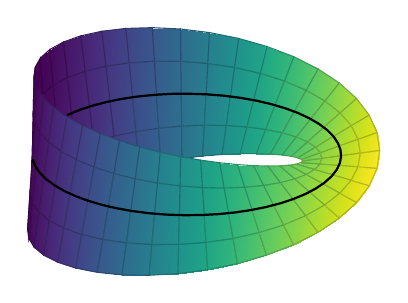
\begin{tikzpicture}
\begin{axis}[scale=0.75,
    hide axis,
    view={10}{40}
]
\addplot3 [
    surf, shader=faceted interp,
    point meta=x,
    colormap/viridis,
    samples=40,
    samples y=5,
    z buffer=sort,
    domain=0:360,
    y domain=-0.5:0.5
] (
    {(1+0.5*y*cos(x/2)))*cos(x)},
    {(1+0.5*y*cos(x/2)))*sin(x)},
    {0.5*y*sin(x/2)});

\addplot3 [
    samples=50,
    domain=-165:150, % The domain needs to be adjusted manually, depending on the camera angle, unfortunately
    samples y=0,
    thick
] (
    {cos(x)},
    {sin(x)},
    {0});
\end{axis}
\end{tikzpicture}$$

    Sea $M = \modulo{([0, 1] \times (0, 1))}{\sim}$ el conjunto de las clases de equivalencia. Considera los subconjuntos $U = \modulo{((0, 1) \times (0, 1))}{\sim}$ y $V =  \modulo{([0, 1] - \{\nicefrac{1}{2}\} \times (0, 1))}{\sim}$. Sean las aplicaciones $\varphi : U \to \mathbb R^2$ y $\psi : V \to \mathbb R^2$ dadas por: 
    $$\varphi([(x,y)]) = (x,y) \qquad \text{ y } \qquad \psi([(x,y)])=\begin{cases}
        (x,y) & \text{ si } x < \nicefrac{1}{2} \\  (x-1,1-y) & \text{ si } x > \nicefrac{1}{2} 
    \end{cases}.$$
    \begin{enumerate}
        \item Demuestra que $\{(U, \varphi), (V, \psi)\}$ es un atlas de $M$.
        \begin{sol}
            En primer lugar, comprobaremos que son cartas. Las aplicaciones ets\'an bien definidas, son inyectivas y las im\'agenes de los subconjuntos son abiertos. En efecto, $\varphi$ est\'a bien definida, pues $(x,y)\sim (x,y)$ solo, por habernos deshecho de los extremos. Adem\'as es inyectiva, ya que $\varphi([(x,y)]) = \varphi \circ \pi (x,y) =(x,y)$, es decir, $\varphi \circ \pi = Id$. As\'i pues, sobre $[0, 1] \times (0, 1)$, se verifica que $\varphi = \pi^{-1}$, luego por ser $\pi$ epiyectiva, $\varphi$ es inyectiva.
            
             $\psi$ est\'a bien definida. Si $x \neq 0,1$ las clases solo tienen un representante. Si $[(0,y)]=[(1,1-y)]$, entonces por $\psi$, $(0,y) = (0,1-(1-y))=(0,y)$
             
            De la misma forma pque en $\varphi$, se demuestra la inyectividad para $\psi$ si $x < \nicefrac{1}{2}$. En el caso en que $x > \nicefrac{1}{2}$, podemos argumentar, en el sentido m\'as elemental de inyectividad que
            $$\psi([(x,y)]) = \psi([(x',y')]) \iff (x-1,1-y)=(x'-1,1-y') \iff  $$
            $$\begin{cases}
                x-1=x'-1 & \Rightarrow x=x' \\ 1-y = 1-y' & \Rightarrow y=y'
            \end{cases} \implies (x,y) \sim (x',y') \iff [(x,y)] = [(x',y')]$$
            Adem\'as, 
            $$\varphi(U)=\pi^{-1}(U) =(0,1) \times (0,1) \qquad \psi(V)= (-\nicefrac{1}{2},\nicefrac{1}{2})  \times (0,1)$$
            que son abiertos en la topología producto (abierto $\times$ abierto).

            El segundo caso se demuestra como sigue:
            \begin{enumerate}
                \item En el conjunto $V_1=\modulo{[0,\nicefrac{1}{2}) \times (0,1)}{\sim}$, es el mismo caso que el anterior, luego 
                $$\psi(V_1) = [0,\nicefrac{1}{2}) \times (0,1)$$
                \item En el conjunto $V_2=\modulo{(\nicefrac{1}{2},1] \times (0,1)}{\sim}$, la aplicaci\'on es $\psi\circ \pi(x,y) = (x-1,1-y)$ de forma que 
                $$\psi(V_2)=(\nicefrac{1}{2}-1,1-1] \times (1,0) = (-\nicefrac{1}{2},0] \times (0,1)$$
            \end{enumerate} 
            de manera que
            $$\psi(V) = \psi(V_1 \cup V_2) = \psi(V_1) \cup \psi(V_2) = [0,\nicefrac{1}{2}) \times (0,1) \cup (-\nicefrac{1}{2},1] \times (0,1) =(-\nicefrac{1}{2},\nicefrac{1}{2}) \times (0,1)$$

            Comprobemos que son atlas. Claramente, $M = U \cup V$ ya que uno cubre lo que otro no. Para comprobar la compatibilidad de la funciones veamos sus inversas. 
            $$\bt 
            \varphi^{-1} : & (0,1) \times (0,1) \arrow{r} & U \\[-5mm] & (x,y) \arrow[mapsto]{r} & \left[(x,y)\right] \\ \psi^{-1}: & (-\nicefrac{1}{2},\nicefrac{1}{2}) \times (0,1) \arrow{r} & V \\[-8mm] 
            & (x,y) \arrow[mapsto]{r} & \begin{cases}
                [x,y] \quad \quad \quad 0 \leq x < \nicefrac{1}{2} \\ [x+1, 1-y] \quad -\nicefrac{1}{2} < x \leq 0
            \end{cases}
            \et$$
            y ahora $U \cap V = \modulo{((0, 1) - \{\nicefrac{1}{2}\} \times (0, 1))}{\sim}$, de forma que 
            $$\psi \circ \varphi^{-1}(x,y) = \psi([x,y])=\begin{cases}
                (x,y) & 0< x< \nicefrac{1}{2} \\ (x-1,1-y)& \nicefrac{1}{2}< x < 1
            \end{cases}$$
            que es diferenciable $\mathcal C^{\infty}$, ya que lo es cada componente conexa, excluyendo $0,1, \nicefrac{1}{2}$. De la misma forma
            $$\varphi^{-1} \circ \psi (x,y)=\begin{cases}
                (x,y) & 0< x< \nicefrac{1}{2} \\ (x-1,1-y)& -\nicefrac{1}{2}< x < 0
            \end{cases}$$
            es tambi\'en diferenciable, y $\{(U,\varphi),(V,\psi)\}$ es un atlas 2-dimensional $\mathcal{C}^{\infty}$ de $M$, pudiendo extenderlo a uno mayor maximal respecto a la condici\'on de compatibilidad.
        \end{sol}
        \item Analiza si est\'an bien definidas y son diferenciables las aplicaciones $f_i : M \to \mathbb R$, $i = 1, 2, 3$, dadas por:
        $$f_1([(x,y)])=y \quad f_2([(x,y)]) = (y-\nicefrac{1}{2})^2 \quad f_3([(x,y)])=\sin(\pi x) \cos(\pi y)$$
        \begin{sol}
            \begin{enumerate}
                \item No est\'a bien definida, ya que para $[(0,\nicefrac{1}{3})] = [(1,\nicefrac{2}{3})]$, $f_1$ asocia a ellos distintas im\'agenes.
                \item Sea una clase con dos respresentantes, $[(0,y)] = [(1,1-y)]$, de forma que su imagen es 
                $$(y-\nicefrac{1}{2})^2 =(1-y-\nicefrac{1}{2})^2 = (\nicefrac{1}{2}-y)^2$$ por lo que est\'a bien definida.
                Veamos si son diferenciables:
                $$f_2 \circ \varphi^{-1}(x,y)=f_2[x,y]=(y-\nicefrac{1}{2})^2$$
                $$f_2 \circ \psi^{-1}(x,y)=\begin{cases}
                    f_2[x+1,1-y] \\ f_2[x,y]
                \end{cases} = \begin{cases}
                    (1-y-\nicefrac{1}{2})^2 & 0\leq x< \nicefrac{1}{2} \\ (y-\nicefrac{1}{2})^2 &  -\nicefrac{1}{2}< x \leq0 
                \end{cases}= (y-\nicefrac{1}{2})^2$$
                que como hemos visto en el caso anterior, es diferenciable. 
                
                \textit{Observaci\'on.} Podr\'ia parecer que no es diferenciable por no coincidir los valores en el punto en el que no est\'a definido, pero es que este abierto total no es conexo, por lo que basta que sea diferenciable en cada componente conexa.
                \item Debería ser diferenciable.
            \end{enumerate}
        \end{sol}
        \item Determina si $g: M \to M$ est\'a bien definida y es diferenciable, donde:
        $$g([(x,y)]) = \left[\left(x,\nicefrac{1}{2}\right)\right]$$
        \begin{sol}
            Tenemos dos casos para $[(x,y)]$. Si $x \neq 0, 1$, entonces est\'a trivialmente bien definida, pues si $(x,y) \sim (x',y')$, entonces $(x,y) =(x',y')$. Ahora bien, si $x=0$, entonces $[x,y] = [x',y']$ con $x'=1$ e $y'=1-y$, es decir, $[(0,y)]=[(1,1-y)]$. Hagamos pues ambas im\'agenes por $g$ es decir, $g[(0,y)]=[(0,\nicefrac{1}{2})]$ y $g[(1,1-y)]=[(1, \nicefrac{1}{2})]$. Adem\'as, est\'an relacionados, ya que $\nicefrac{1}{2} = 1-\nicefrac{1}{2}$. Tambi\'en $g([x,y]) \in M$. As\'i concluimos que est\'a bien definida. 

            Para demostrar la diferenciabilidad, hacemos la composici\'on con la inversa de las cartas, si $p=[x,y] \in U$, entoces $g(p)\in U $podemos utilizar la lectura en coordenadas, es decir
            $$\varphi \circ g \circ \varphi^{-1}(x,y) = \varphi\circ g([x,y]) = \varphi([(x,\nicefrac{1}{2})])=(x,\nicefrac{1}{2})$$
            Para los $p=[0,y] \in V$, $g(p) \in V$
            $$\psi \circ g \circ \psi^{-1}(x,y) = \begin{cases}
                \psi (g([(x+1,1-y)]))  \\ 
                \psi (g([(x,y)]))     
            \end{cases} = \begin{cases}
                \psi([(x+1,\nicefrac{1}{2})])  &  \text{ si }-\nicefrac{1}{2}< x \leq 0   \\ 
                \psi([(x,\nicefrac{1}{2})])     & \text{ si }0\leq x< \nicefrac{1}{2} 
            \end{cases} $$
            $$=(x,\nicefrac{1}{2})$$
            que son diferenciables.
        \end{sol}
    \end{enumerate}
\end{ejer}
\section{Seminario 3. 3 de octubre}
\begin{ejer} [2]
    \textit{Ejercicio 1.18.} En el espacio vectorial de las matrices cuadradas $Mat_{n\times n}(\mathbb R)$ demuestra que son diferenciables las aplicaciones: suma de matrices, producto de
    matrices, trasposici\'on, traza y determinante. Demuestra que $GL(n, \mathbb R) = \{A \in Mat_{n\times n}(\mathbb R) \, / \, det A \neq 0 \}$ es un abierto de $Mat_{n\times n}(\mathbb R)$.
\end{ejer}
\begin{sol}
    Dado que $Mat_{n \times n}(\mathbb R) \simeq \mathbb R^{n^2}$, dotaremos a $Mat_{n \times n}(\mathbb R)$ de la estructura diferenciable generada por el atlas usual de $\mathbb R^{n^2}$, que es $\{(\mathbb R^{n^2}, Id)\}$. As\'i pues, para comprobar que son diferenciables las aplicaciones no hace falta ni comprobar la composici\'on, pues la \'unica carta del atlas es $(\mathbb R^{n^2}, Id)$. 

    Tambi\'en podemos definir la base est\'andar $\{E_{ij}\}_{1\leq i,j \leq n}$ siendo $E_{ij}$ la matriz con todo ceros y un 1 en el lugar $ij$ y para $A=(a_{ij})$ la aplicaci\'on $\varphi(A)=(a_{11}, \ldots, a_{nn})$ (el isomorfismo.)
    
    Usando el isomorfismo mencionado, podremos expresar las aplicaciones en coordenadas, por la correspondencia:
    $$Mat_{n \times n}(\mathbb R)  \ni\begin{pmatrix} a_{11} & \cdots & a_{1n} \\ \vdots & \ddots & \vdots \\ a_{n1} & \cdots & a_{nn} 
    \end{pmatrix} \leadsto (a_{11}, \ldots, a_{1n}, a_{21},  \ldots,  a_{2n}, \ldots, a_{n1}, \ldots, a_{nn} ) \in \mathbb R^{n^2}$$
    as\'i, tenemos las siguientes aplicaciones:
    \begin{itemize}
        \item Suma de matrices
        $$f(A,B) = A+B = (a_{ij} + b_{ij})_{i,j \in I}$$
        con $I=\{1, \ldots, n\}$. Claramente es diferenciable, por ser sumas.
        \item Producto de matrices
        $$f(A,B) = A \cdot B= (\sum_{i,j=1}^n a_{ij} \cdot b_{ji})_{i,j}$$
        Es diferenciable por ser sumas y productos.
        \item Trasposici\'on
        $$f(A)=A^t = (a_{ji})$$
        para todo $j \neq i$. Diferenciable por ser una permutaci\'on.
        \item Traza
        $$f(A)=\sum_{i=1}^n a_{ii}$$
        diferenciable por ser suma.
        \item Determinante
        $$f(A)=det(A)= \sum_{\sigma \in S_n} signo(\sigma) \prod_{i=1}^n a_{i, \sigma(i)}$$
        que es tambi\'en diferenciable por ser suma, productos y trasposiciones de elementos. 
        
        Como la aplicaci\'on $det$ es diferenciable, es continua, y por tanto la antiimagen de un abierto es un abierto, y tambi\'en la de un cerrado, luego $det^{-1}(\{0\}) = \{A \in Mat_{n\times n}(\mathbb R) \, / \, det A = 0 \} =Mat_{n \times n}(\mathbb R) - Gl(n, \mathbb R)$ es un cerrado, luego su complementario es $Gl(n, \mathbb R)$ ser\'a abierto. De esta forma, $Gl(n, \mathbb R)$ es una variedad diferenciable.
    \end{itemize}
\end{sol}
\begin{ejer}
    [3] Considera las aplicaciones $f : \mathbb RP^2 \to \mathbb RP^2$ y $\sigma : (0, +\infty) \to \mathbb RP^2$ dadas por las
    expresiones:
    $$f([(x_o,x_1,x_2)]) = [(x_o^2+x_1^2, x_o^2+x_2^2,x_1x_2)] \quad \text{ y } \quad \sigma(t) = [(t^{\nicefrac{1}{2}}, t , t^{\nicefrac{3}{2}})]$$
    Demuestra que est\'an bien definidas y son diferenciables.
\end{ejer}
\begin{sol}
    Consideremos el primer caso. Se sabe que $[(x_o,x_1,x_2)] = [(x'_o,x'_1,x'_2)] \iff (x_o,x_1,x_2)=(\lambda x_o,\lambda x_1,\lambda x_2)$.  Hagamos ambas im\'agenes por $f$:
    $$f([(\lambda x_o,\lambda x_1,\lambda x_2)]) = [(\lambda^2 x_o^2 + \lambda ^2 x_1^2, \lambda^2 x_o^2 + \lambda ^2 x_2^2, \lambda x_1 \lambda x_2)] = [(\lambda^2 (x_o^2 + x_1^2), \lambda^2 (x_o^2 + x_2^2), \lambda^2 x_1 x_2)] = $$
    $$= [\lambda^2(x_o,x_1,x_2)]=[(x_o,x_1,x_2)]=f([(x_o,x_1,x_2)])$$
    por lo que está bien definida. La aplicaci\'on $\sigma$ est\'a bien definida, pues es una aplicaci\'on de $\mathbb R^+$ en $\mathbb RP^2$ definida en todo punto.

    Para comprobar la diferenciabilidad, lo haremos con las cartas de $\mathbb RP^2$ dadas por el atlas $\{V_i, \phi_i\}$ con $V_i = \{[x_o,x_1,x_2] \in \mathbb RP^2\, /\, x_i \neq 0\}$. En tal caso, $\phi_i \circ f \circ \phi_j^{-1}$ ser\'a diferenciable, $\forall i,j = 0,1,2$

    De la misma forma, $\phi_i \circ \sigma $ con $ i = 0,1,2$.  
\end{sol}
\section{Expo 10 de octubre}
\begin{ejer}
    [1] Considera la aplicaci\'on $f: \bold S^2 \longrightarrow \bold S^2$ y la curva $\sigma(t): \mathbb R \longrightarrow \bold S^2$ dadas por las expresiones:
$$f(x,y,z)=\left( \dfrac{1}{2} x\, \sin \, y, \dfrac{1}{2}x \cos \, y, \sqrt{\dfrac{y^2+z^2}{4}+\dfrac{3}{4}}\right)$$
$$ \sigma(t) = \left(\dfrac{2t \cos(t)}{1 + t^2} ,\dfrac{2t \sin(t)}{ 1 + t^2}, \dfrac{t^2-1}{1+t^2}\right)$$ Demuestra que est\'an bien definidas y son diferenciables.
\end{ejer}
\begin{ejer}
    [2] Si $M$ denota la banda de Moebius, considera la aplicaci\'on $f : M \times \mathbb R \longrightarrow \mathbb R^2$ y la curva $\sigma : (-\nicefrac{\pi}{2}, \nicefrac{3\pi}{2}) \longrightarrow M$ dadas por las expresiones:
    $$f([x,y],z)=(\cos (2\pi x)\sin(z),(y-\nicefrac{1}{2})^2 \cos(z)),$$
    $$\sigma(t)=\begin{cases}
        [(\frac{1}{\pi}t+\frac{1}{2}, \frac{1}{2}+\frac{1}{3}\sin t)] \quad t \in (-\nicefrac{\pi}{2},\nicefrac{\pi}{2}] \\  [(\frac{1}{\pi}t-\frac{1}{2}, \frac{1}{2}-\frac{1}{3}\sin t)] \quad t \in [\nicefrac{\pi}{2},\nicefrac{3\pi}{2}])
    \end{cases}$$
Demuestra que est\'an bien definidas y son diferenciables.
\end{ejer}
\section{Expo 24 de octubre}
\begin{ejer} [1] Considera la curva $\sigma : \mathbb R \longrightarrow \bold S^2:$
$$ \sigma(t) = \left(\dfrac{2t \cos(t)}{1 + t^2} ,\dfrac{2t \sin(t)}{ 1 + t^2}, \dfrac{t^2-1}{1+t^2}\right)$$
de la sesi\'on anterior, que sabemos es diferenciable. Calcula $\sigma'(t)$ en coordenadas estereogr\'aficas de $\bold S^2$. Si $f : \bold S^2 - \{(0, 0, \pm1)\} \longrightarrow \mathbb R$ es la funci\'on diferenciable $f(x, y, z) = \frac{xy}{1-z^2}$, calcula $\sigma'(t)(f)$ para $t = 0$ y para $t = \nicefrac{\pi}{4}$.
\end{ejer}
\begin{sol}
Recordemos que las coordenadas estereogr\'aficas de $\bold S^2$ son $(\bold S^2-\{N\}, \varphi_N), (\bold S^2-\{S\}, \varphi_S)$, siendo $N, S$ el polo norte y sur y las aplicaciones
$$\begin{array}{rrcl}
                     \varphi_N : & \bold S^2 - \{N\} & \longrightarrow & \mathbb R^2  \\
                     &(x_1,x_2,x_3) & \longmapsto & (u_1,u_2)=\left( \dfrac{x}{1-z}, \dfrac{y}{1-z}\right) 
                \end{array}\hspace{45mm}$$
$$\begin{array}{rrcl}
                     \varphi_N^{-1} : & \mathbb R^2 & \longrightarrow & \bold{S}^2  \\
                     &(x,y) & \longmapsto & (x,y,z) = \left( \dfrac{2u_1}{1 + u_1^2 + u_2^2} , \dfrac{2u_2}{1 + u_1^2 + u_2^2}, \dfrac{-1 + u_1^2 + u_2^2}{1 + u_1^2 + u_2^2}\right)
                \end{array} $$
$$\begin{array}{rrcl}
                     \varphi_S : & \bold S^2 - \{S\} & \longrightarrow & \mathbb R^2  \\
                     &(x_1,x_2,x_3) & \longmapsto & (v_1,v_2)=\left( \dfrac{x}{z+1}, \dfrac{y}{z+1}\right) 
                \end{array}\hspace{45mm}$$ 
                $$\begin{array}{rrcl}
                     \varphi_S^{-1} : & \mathbb R^2 & \longrightarrow & \bold S^2 - \{S\}  \\
                     & (x,y) & \longmapsto & (z,y,z) = \left( \dfrac{2v_1}{1 + v_1^2 + v_2^2} , \dfrac{2v_2}{1 + v_1^2 + v_2^2}, \dfrac{1 - v_1^2 - v_2^2}{1 + v_1^2 + v_2^2}\right) \end{array}$$
En primer lugar, como $\frac{t^2-1}{1+t^2} \neq 1$, entonces $\sigma(\mathbb R)\subset \bold S^2- \{0,0,1\}$, es decir, podemos usar la carta del polo norte. Por lo tanto, $\left\{\frac{\partial}{\partial u_1}\big|_{\sigma(t)}, \frac{\partial}{\partial u_2}\big|_{\sigma(t)}\right\}$ es una base de $T_{\sigma(t)}\bold S^2$, y por tanto
$$\sigma'(t)=\dfrac{d}{dt} (u_1\circ \sigma) \, \pd{}{u_1}\Big|_{\sigma(t)}+ \dfrac{d}{dt} (u_2\circ \sigma) \, \pd{}{u_2}\Big|_{\sigma(t)}$$
\begin{itemize}
    \item $(u_1\circ \sigma) = (r_1 \circ \varphi \circ \sigma )$
    $$(u_1 \circ \sigma)(t) = \dfrac{\frac{2t \cos(t)}{1+t^2}}{1-\frac{t^2}{1+t^2}} = \dfrac{\frac{\cancel{2} t \cos(t)}{\cancel{1+t^2}}}{\frac{\cancel{2}}{\cancel{1+t^2}}} = t \cos(t)$$
    por lo que derivando
    $$\dfrac{d}{dt}(t \cos(t)) = \cos(t) - t \sin (t)$$
    \item  $(u_2\circ \sigma) = (r_2 \circ \varphi \circ \sigma )$
    $$(u_2 \circ \sigma)(t) = \dfrac{\frac{2t \sin(t)}{1+t^2}}{1-\frac{t^2}{1+t^2}} = \dfrac{\frac{\cancel{2} t \sin(t)}{\cancel{1+t^2}}}{\frac{\cancel{2}}{\cancel{1+t^2}}} = t \sin(t)$$
    por lo que derivando
    $$\dfrac{d}{dt}(t \sin(t)) = \sin(t) + t \cos (t)$$
\end{itemize}
y recopilando, la expresi\'on de $\sigma'(t)$ en coordenadas estereog\'raficas es 
$$\sigma'(t)=\dfrac{d}{dt} \big(\cos(t) - t \sin (t)\big) \, \pd{}{u_1}\Big|_{\sigma(t)}+ \dfrac{d}{dt} \big(  \sin(t) + t \cos (t) \big) \, \pd{}{u_2}\Big|_{\sigma(t)}$$

As\'i pues, calcular lo \'ultimo es tan sencillo como hallar 
$$\dfrac{d(f\circ \sigma)}{dt} \Big|_t $$
y aplicar a los distintos valores de $t$. As\'i, 
$$(f \circ \sigma)(t) = \dfrac{\frac{2t \cos(t)}{1 + t^2} \cdot\frac{2t \sin(t)}{ 1 + t^2}}{1-\left(\frac{t^2-1}{1+t^2}\right)^2}=\dfrac{\frac{4t^2 \sin t \cos t}{\cancel{(1+t^2)^2}}}{\frac{\cancel{1}+2t^2+\cancel{t^4} - \cancel{t^4} + 2t^2 - \cancel{1}}{\cancel{(1+t^2)^2}}} = \dfrac{4t^2 \sin t \cos t}{4t^2} =  \sin t \cos t$$
luego
$$\dfrac{d(f\circ \sigma)}{dt} \Big|_t = \dfrac{d(\sin t \cos t)}{dt} \Big|_t = \cos^2(t) - \sin^2(t) $$
por lo que
$$\sigma'(0)(f) = \cancelto{1}{\cos^2(0)} - \cancelto{0}{\sin^2(0)} = 1 \qquad \sigma'(\nicefrac{\pi}{4})(f) = \cos^2(\nicefrac{\pi}{4}) - \sin^2(\nicefrac{\pi}{4}) = (\nicefrac{\sqrt{2}}{2})^2 - (\nicefrac{\sqrt{2}}{2})^2  =0$$
\end{sol}
\begin{ejer}
    [2] Sea $M$ la banda de Moebius, y considera la aplicaci\'on $f : M \times \mathbb R \longrightarrow \mathbb R^2$:
    $$f([x,y],z)=\left( \cos(2\pi x) \sin(z), (y-\nicefrac{1}{2})^2 \cos(z)\right)$$
    de la sesi\'on anterior, que sabemos es diferenciable. Calcula el jacobiano de $f$ en los puntos de la forma $p = ([\nicefrac{1}{2},y],0)$ y $q=([0,\nicefrac{1}{3}],z)$.
\end{ejer}
\begin{sol}
Recordemos el atlas $(U,\varphi), (V, \psi)$ que hab\'iamos utilizado para la banda de Moebius, donde  $U = \modulo{((0, 1) \times (0, 1))}{\sim}$ y $V =  \modulo{([0, 1] - \{\nicefrac{1}{2}\} \times (0, 1))}{\sim}$ y las aplicaciones:
$$\varphi([(x,y)]) = (x,y) \qquad \text{ y } \qquad \psi([(x,y)])=\begin{cases}
        (x,y) & \text{ si } x < \nicefrac{1}{2} \\  (x-1,1-y) & \text{ si } x > \nicefrac{1}{2} 
    \end{cases}.$$
$$\bt \varphi^{-1} : (0,1) \times (0,1) \arrow{r} & U \\[-5mm]  (x,y) \arrow[mapsto]{r} & \left[(x,y)\right] \et $$
y dado que $f$ tiene como espacio de salida $M \times \mathbb R$, haremos una modificaci\'on de estas, de forma que $U' = \modulo{((0, 1) \times (0, 1))}{\sim} \times \mathbb R$ y $V' =  \modulo{([0, 1] - \{\nicefrac{1}{2}\} \times (0, 1))}{\sim}  \times \mathbb R$ y las aplicaciones ser\'an:
$$\varphi'([(x,y)],z) = (x,y,z) \qquad \text{ y } \qquad \psi'([(x,y)],z)=\begin{cases}
        (x,y,z) & \text{ si } x < \nicefrac{1}{2} \\  (x-1,1-y,z) & \text{ si } x > \nicefrac{1}{2} 
    \end{cases}$$
$$\bt (\varphi')^{-1} :  (0,1) \times (0,1)  \times \mathbb R \arrow{r} & U' \\[-5mm]  (x,y,z) \arrow[mapsto]{r} & (\left[(x,y)\right],z) \et $$
Podemos comprobar f\'acilente que $p \in U'$ pero $p \nin V'$ y que $q \nin U'$ pero $q \in V'$, por lo que para $p$ deberemos expresar el jacobiano en coordenadas $(U', \varphi')$ y $q$ en $(V', \psi')$. Pero si nos damos cuenta, $q$ tiene $x<\nicefrac{1}{2}$, luego $\psi' = \varphi'$, y la lectura en coordenadas ser\'a la misma.

Para calcular el jacobiano en $p$ y $q$, calcularemos la lectura en coordenadas de $f$:
$$Id \circ f \circ (\varphi')^{-1} = (\cos(2\pi x)\sin(z) = f_1,(y-\nicefrac{1}{2})^2 \cos(z) = f_2 )$$
luego el jacobiano es 
$$(Jf)_s \leadsto \begin{pmatrix}
    \pd{f_1}{x}\Big|_{s} & \pd{f_1}{y}\Big|_{s}  & \pd{f_1}{z}\Big|_{s}  \\[3mm]  \pd{f_2}{x}\Big|_{s}  & \pd{f_2}{y}\Big|_{s}  & \pd{f_2}{z}\Big|_{s} 
\end{pmatrix} = \begin{pmatrix}
    -2\pi\sin(z)\sin(2\pi x) & 0 & \cos(2\pi x) \cos(z) \\ 0 &(2y-1) \cos(z) & -(y-\nicefrac{1}{2})^2 \sin(z)
\end{pmatrix}$$
    por lo que 
    $$(Jf)_p\leadsto \begin{pmatrix}
        0 & 0 & -1 \\ 0 & 2y-1 & 0
    \end{pmatrix}\qquad (Jf)_p\leadsto \begin{pmatrix}
        0 & 0 & \cos(z) \\ 0 & -\frac{\cos(z)}{3} & -\frac{\cos(z)}{36}
    \end{pmatrix}$$
\end{sol}
\section{Expo 7 de noviembre}
\begin{ejer}
    [1] Sea $M$ la banda de Moebius y considera las funciones $f_i:M \longrightarrow \mathbb R, \, i=1,2$:
    $$f_1\left([(x,y)]\right) = (2y-1) \cos \, \pi x\quad \text{ y } \quad f_2\left([(x,y)]\right) =(2y-1)\sin \, \pi x$$
Determina un abierto de $M$ (lo m\'as grande posible) donde $\{f_1, f_2\}$ formen un
sistema de coordenadas.
\end{ejer}
\begin{sol} Como si $(JF)_p$ es de rango m\'aximo, $\{d_pf_1, d_pf_2\}$ son l.i., en $W = \{[(x,y)] \in M \, / \, y \neq \nicefrac{1}{2}\}$, y entonces $\exists \Tilde{W} \subset W$ abierto con $p \in \Tilde{W}$ tal que $(\tilde{W}, F|_{\tilde{W}})$ es carta. Como $F|_W$ es inyectiva, entonces $F(W)$ es abierto y $F|_W:W \longleftarrow F(W)$ es difeomorfismo. 
\end{sol}
\begin{ejer}
    [2] En el plano proyectivo $\mathbb RP^2$, considera las funciones dadas por las expresiones:
 $$f_1[(x_o, x_1, x_2)] = \dfrac{x_o}{x_1 + x_2} \quad \text{ y } \quad f_2[(x_o, x_1, x_2)] = \dfrac{x_1}{x_o + x_2}$$
Determina un abierto $U \subset \mathbb RP^2$ (lo m\'as grande posible) donde $(U, f = (f_1, f_2)$ sea una carta de $\mathbb RP^2$.
\end{ejer}
\begin{sol}
    Como $\{d_pf_1, d_pf_2\}$ son l.i., busquemos el abierto m\'as grande en que son. Sea $$W=\{[x_o,x_1,x_2] \in \mathbb RP^2 \, / \,  x_o+x_2\neq0, x_1+x_2\neq 0\, x_o+x_1+x_2 \neq 0\}$$ 
    de forma que veamos si $F=(f_1,f_2)$ es inyectiva en $W$. 

    Sea $p, q \in W \cap V_o \cap V_1 \cap V_2$, $p=[x_o,x_1,x_2], \, q=[x_1',x_2',x_3']$, por lo que existen $\alpha, \beta, \gamma \in \mathbb R^+$ tal que $x_o'=\alpha x_o, x_1'=\beta x_1, x_2'=\gamma x_2$. De esta forma, 
    $$\begin{cases}
        \dfrac{x_o}{x_1+x_2}=\dfrac{x_o'}{x_1'+x_2'} = \dfrac{\alpha x_o}{\beta x_1+\gamma x_2} & \Rightarrow (\beta x_1 + \gamma x_2) = \alpha(x_1+x_2) \\ \dfrac{x_1}{x_o+x_2} = \dfrac{\beta x_1}{\alpha x_o + \gamma x_2} & \Rightarrow \begin{cases}
            \gamma=(\alpha- \beta)\frac{x_1}{x_2}+\alpha \\ (\alpha-\beta)(x_1+x_1+x_2)=0 \Rightarrow \alpha = \beta \Rightarrow \gamma=\alpha
        \end{cases}
    \end{cases}$$
    por lo que en $W \cap V_o$
    $$F\circ \phi_o (u_o,u_2) = F\circ \phi(v_1,v_2) \Rightarrow u_1=v_1, \, u_2=v_2$$
    De la misma forma en $W\cap V_1, W\cap V_2$, es decir, es inyectiva en todo $W$. 
\end{sol}
\section{Expo 21 de noviembre}
\begin{ejer}
    [1] Ya vimos que la aplicaci\'on
    $$\begin{array}{rrcl}
         f : & \bold S^2 & \longrightarrow & \bold S^2  \\
         & (x,y,z) & \longmapsto & \left( \dfrac{1}{2} x\, \sin \, y, \dfrac{1}{2}x \cos \, y, \sqrt{\dfrac{y^2+z^2}{4}+\dfrac{3}{4}}\right) 
    \end{array}$$
    es diferenciable. Determina todos los puntos en los que $f$ es inmersi\'on. \textit{Sugerencia: usa las proyecciones ortogonales.}
\end{ejer}
\begin{sol}
    De la definici\'on, si $p \in U_3^{\pm}$, es decir, si $p \in U_3^+$ \'o $p \in U_3^-$, 
    \[ \begin{split} \psi_3^+ \circ f \circ (\psi_3^{\pm})^{-1} & = (x,y,\pm \sqrt{1-x^2-y^2}) = \psi_3^+ \left( \dfrac{1}{2} x\, \sin \, y, \dfrac{1}{2}x \cos \, y, \sqrt{1-x^2} \right) = \\ & =  \left( \dfrac{1}{2} x\, \sin \, y, \dfrac{1}{2}x \cos \, y \right) \end{split}\]
     de forma que 
    $$Jf = \begin{pmatrix}
        \nicefrac{1}{2} \sin y & \nicefrac{1}{2} x \cos y \\ \nicefrac{1}{2} \cos y & -\nicefrac{1}{2}x \sin y
    \end{pmatrix} \Rightarrow |Jf| = - \dfrac{1}{4} x$$
    es decir, ser\'a de rango m\'aximo cuando $x\neq 0$. As\'i, $\forall p\in S \, / \,  x\neq 0$, $f$ es inmersi\'on en $p$. Para otros casos, sea $p \in U_2^{\pm}$,
    \[ \begin{split}
        \psi_3^+ \circ f \circ (\psi_2^{\pm})^{-1}(x,y,z) & = \psi_3^+ \left( f (x,\pm \sqrt{1-x^2+z^2}, z)\right) = \\ & = \psi_3^+ \left( \dfrac{1}{2} x\, \sin \, \left(\pm \sqrt{1-x^2+z^2}\right), \dfrac{1}{2}x \cos \, \left(\pm \sqrt{1-x^2+z^2}\right), \cdots \right) = \\ & = \left( \dfrac{1}{2} x\, \sin \, \left(\pm \sqrt{1-x^2+z^2}\right), \dfrac{1}{2}x \cos \, \left(\pm \sqrt{1-x^2+z^2}\right) \right)
    \end{split} \]
    luego 
    $$(Jf)_p=\begin{pmatrix}
        \sin \left(\pm \sqrt{1-x^2+z^2}\right) \pm x \cos \left(\pm \sqrt{1-x^2+z^2}\right) \frac{-x}{\sqrt{1-x^2+z^2}} & \pm \cos \left(\sqrt{1-x^2+z^2}\right) \frac{-z}{\sqrt{1-x^2+z^2}} \\ 
        \cos\left( \sqrt{1-x^2+z^2}\right) + \sin \left(\sqrt{1-x^2+z^2}\right) \frac{x}{\sqrt{1-x^2+z^2}} & x \sin \left(\sqrt{1-x^2+z^2}\right) \frac{z}{\sqrt{1-x^2+z^2}}
    \end{pmatrix}$$
    $$|Jf|_p = \dfrac{xz}{2 \sqrt{1-x^2-z^2}} = 0 \iff \begin{cases}
        x = 0 \\ \text{ \'o } \\ z=0
    \end{cases}$$

    En el \'ultimo caso, si $p \in U_1^{\pm}$, se calcula que $|Jf|_p = \mp \dfrac{z}{4}$, es decir, es nulo si $z=0$. 

    Concluimos as\'i que no es una inmersi\'on en todos los puntos, pues se excluyen aquellos en los que $x=0$ y $z=0$.
\end{sol}
\begin{ejer}
    [2] \textit{Ejercicio 3.29} Considera el abierto $U = V_o\cap V_1 \cap V_2 = \{[(x_o, x_1, x_2)] \in \mathbb RP^2 | x_ox_1x_2 \neq 0\}$ de $\mathbb RP^2$ y la aplicaci\'on $f : U \to \mathbb R$ dada por:
    $$f([(x_o,x_1,x_2)]) = \dfrac{x_o}{x_1}+\dfrac{x_1}{x_2}+\dfrac{x_2}{x_o}$$
    Demuestra que $M = \{[(x_o, x_1, x_2)] \in U \,|\,  f([(x_o, x_1, x_2)]) = 0\}$ es una subvariedad de $U$. Calcula una base de $T_pM$ para $p \in M$ un punto arbitrario.
\end{ejer}
\begin{sol}
    Comprobemos en primer lugar que $f$ est\'a bien definida. Por la relaci\'on en $\mathbb RP^2$, se debe verificar que $f([x_i])=f([\lambda x_i])$. En efecto,
    $$\dfrac{\lambda x_o}{\lambda x_1}+\dfrac{\lambda x_1}{\lambda x_2}+\dfrac{\lambda x_2}{\lambda x_o} = \dfrac{x_o}{x_1}+\dfrac{x_1}{x_2}+\dfrac{x_2}{x_o}$$
    y entonces $M=f^{-1}(0)$, pudiendo hacer la lectrura en coordenadas de $f$ con alguna de las cartas del atlas $\{(V_i, \varphi_i)\}_{i=0}^2$. Eligiendo la primera, 
    $$f\circ \phi_o^{-1}=\dfrac{1}{u} + \dfrac{u}{v}+v$$
    vemos que $f$ es diferenciable en $U$, pues $V_o \subset U$. As\'i pues
    $$d_pf=\pd{}{u}(f\circ \phi_o^{-1})\Big|_p  d_pu +\pd{}{v} (f\circ \phi_o^{-1})\Big|_p d_pv = \left(\dfrac{1}{v}-\dfrac{1}{u^2}, 1-\dfrac{u}{v^2}\right)$$
    y hemos de ver que $\{d_pf\}$ es l.i., lo cual es equivalente a que $d_pf\neq 0$:
    $$\begin{cases}
      \dfrac{1}{v}-\dfrac{1}{u^2}=0 \\[5mm] 1-\dfrac{u}{v^2}  =0
    \end{cases} \iff \begin{cases}
        u^2=v^2 \\ v^2=u
    \end{cases} \iff \begin{cases}
        u=v=0 \\ \text{ \'o } \\ u=v=1
    \end{cases}$$
    y por tanto, $M$ es subvariedad si y solo si $p\neq(1,1), (0,0)$.

    Por un lado, $p=(0,0)\nin M$, pues $f$ se define en $U$, donde $x_ox_1x_2\neq 0$. Por otro lado, si consideramos $p=(1,1)$, $f(\phi_o^{-1}(p))=f(1:1:1)=3\neq 0$, luego $(1,1)\nin M$.

    Calculemos ahora la base de $T_pM$. Sea $p\in M$, se define $T_pM=\{v \in T_p\mathbb R^3 \, /\, v(f)=0\}$, siendo
    $$v=\lambda_1 \pd{}{u}\Big|_p + \lambda_2 \pd{}{v}\Big|_p = \lambda_2 \left( \dfrac{1-\frac{u}{v^2}}{\frac{1}{u^2}-\frac{1}{v}}\right)\pd{}{u}\Big|_p + \lambda_2 \pd{}{v}\Big|_p  $$
    pues 
    $$v(f)=0 \iff \lambda_1 \pd{}{u}\Big|_p(f\circ \phi_o^{-1}) + \lambda_2 \pd{}{v}\Big|_p (f\circ \phi_o^{-1}) = 0 \iff $$
    $$\lambda_1 \left(\dfrac{1}{v}-\dfrac{1}{u^2}\right) + \lambda_2\left( 1-\dfrac{u}{v^2}\right)=0 \iff \lambda_1=\lambda_2 \left( \dfrac{1-\frac{u}{v^2}}{\frac{1}{u^2}-\frac{1}{v}}\right)$$
    y por tanto, 
    $$T_pM = \left\langle  \dfrac{1-\frac{u(p)}{v^2(p)}}{\frac{1}{u^2(p)}-\frac{1}{v(p)}} \pd{}{u}\Big|_p +\pd{}{v}\Big|_p \right\rangle = \cdots = \left\langle (u^2-v^2,v^2)\right\rangle$$
\end{sol}
\section{Expo 5 de diciembre}
\begin{ejer}
    [1] Sea $f : \R^2 \to \R P^2$ la aplicaci\'on diferenciable dada por $f(x, y) = [(1, x + y, x - y)]$, y considera el campo:
    $$X=y\pd{}{x}-x\pd{}{y} \in \mathfrak X(\R^2)$$
   Para todo $p \in \R^2$, expresa $f_{*,p}(X_p)$ en coordenadas del atlas usual $\{(V_i, \phi_i)\}_{i=0}^2$. Generaliza la expresi\'on obtenida para definir un campo $Y \in \X(V_o)$ de modo que $X\overset{f}{\sim} Y$. Sea ahora 
   $$Z=v_1v_2 \pd{}{v_1} + (1+v_2^2)\pd{}{v_2} \in \X(V_1)$$
   donde $\phi_1= (b_1,v_2)$. Comprueba tambi\'en que $X \overset{f}{\sim} Z$. 
\end{ejer}
\begin{sol}
    $\forall p \in \R^2$, $f_{*,p}(X_p)$ usamos la carta $(V_o,\phi_o)$ en $\R P^2$, 
    $$\phi_o \circ f(x,y) = \phi_o [1,x+y,x-y] = (x+y,x-y)$$
    que es diferenciable. Calculamos la matriz jacobiana $$(Jf)_p = \begin{pmatrix}
        1 & 1 \\ 1 & -1
    \end{pmatrix}$$
    entonces
    $$f_{*,p}(X_p)= \begin{pmatrix}
        1 & 1 \\ 1 & -1
    \end{pmatrix}\begin{pmatrix}
        y \\ -x 
    \end{pmatrix}_p = (y-x) \pd{}{u_1}\Big|_{f(p)} + (y+x) \pd{}{u_2}\Big|_{f(p)}$$
    Buscamos un campo  $Y \in \X(V_o) \, / \, Y_{f(p)}=f_{*,p}(X_p)$, en tal caso $X \overset{f}{\sim} Y$. Es decir, 
    $$Y_p = \lambda(u_1,u_2) \pd{}{u_1}\Big|_p + \mu(u_1,u_2) \pd{}{u_2} \Big|_p \qquad \lambda, \mu \in \mc C^{\infty}$$
    y podemos tomar
    $$Y_p = -u_2 \pd{}{u_1}\Big|_p + u_1 \pd{}{u_2}\Big|_p \in \X(V_o)$$
    y se cumple que $f_{*,p}(X_p)=Y_{f(p)} \forall p \in \R^2 \, / \, f(p) \in V_o$. Esto siempre se puede hacer cuando $f$ sea una inmersi\'on, por el Teorema de Estructura Local.
\end{sol}
\begin{ejer}
    [2] Identifica los abiertos $D_t \subset \R^2, \, t \in \R$, para que las aplicaciones $\tau_t : D_t \longrightarrow \R^2$ dadas por:
    $$\tau_t(x,y) = \left(1+\dfrac{2(x-1)e^{2t}}{1+x+(1-x)e^{2t}},\dfrac{2ye^{t}}{1+x+(1-x)e^{2t}}\right)$$
formen un grupo local uniparam\'etrico de transformaciones $\{\tau_t\}_{t\in \R}$. Calcula su generador
infinitesimal.
\end{ejer}\begin{sol}
   $\tau_t(x,y)$ estar\'a definido cuando $1+x+(1-x)e^{2t} \neq 0$, despejando $x$,
    $$x\neq \dfrac{1+e^{2t}}{e^{2t}-1}\qquad t\neq 0$$
    si $t=0$, $D_o = \R^2$. Es decir, $D_t = \left\{ (x,y) \in \R^2 \, / \, x\neq \dfrac{1+e^{2t}}{e^{2t}-1}\right\}$ que es abierto por ser el complementario de un cerrdo, los 0's de una funci\'on.

    Veamos si $\displaystyle\bigcup_{t> 0} D_t= \R^2 = \bigcap_{t<0} D_t$. La primera $\subseteq$ es clara. Veamos la primera $\supseteq$. Dado $(x,y) \in \R^2$, buscamos $t>0 \, / \,  (x,y) \in D_t$. Por ejemplo, con $t=1$. Si $x=\frac{1+e^2}{e^2-1}$, entonces $(x,y)\nin D_1$, entonces $x\neq \dfrac{1+e^4}{e^4-1}$ y por tanto $(x,y) \in D_2$.

    Veamos si es global o local. Calculemos $\tau_o(x,y) = \left(1+(x-1),y \right) = (x,y)$. 

    \[\begin{split} \tau_s(\tau_t(x,y)) & = \tau_s\left(1+\dfrac{2(x-1)e^{2t}}{1+x+(1-x)e^{2t}},\dfrac{2ye^{t}}{1+x+(1-x)e^{2t}}\right)= \\ & = \left(1+\dfrac{2(\frac{2(x-1)e^{2t}}{1+x+(1-x)e^{2t}})e^{2s}}{1+1+\frac{2(x-1)e^{2t}}{1+x+(1-x)e^{2t}}+(\frac{2(x-1)e^{2t}}{1+x+(1-x)e^{2t}})e^{2s}},\right. \\ & \left.\dfrac{2\frac{2ye^{t}}{1+x+(1-x)e^{2t}}e^{s}}{1+(1+\frac{2(x-1)e^{2t}}{1+x+(1-x)e^{2t}})+(\frac{2(x-1)e^{2t}}{1+x+(1-x)e^{2t}})e^{2s}}\right) = \\ & =
    \left( 1+\dfrac{4(x-1)e^2t e^{2s}}{2(1+x+\cancel{(1-x)e^{2t}})+\cancel{2(x-1)e^{2t}} - 2(x-1)e^{2t}e^{2s}}\right., \\& 
    \left. \dfrac{4ye^te^s}{2(1+x+(1-x)e^{2t})+2(x-1)e^{2t} - 2(x-1)e^{2t}e^{2s}}\right) = \\ & = 
    \left( 1+\dfrac{2(x-1) e^{2(t+s)}}{1-x+(1-x) e^{2(t+s)}}, \dfrac{2ye^{t+s}}{1+x+(1-x)e^{2(t+s)}}\right) = \\ & = \tau_{t+s}(x,y)
    \end{split}\]

    Calculamos el generador infinitesimal, es decir, el campo del que proviene el grupo local uniparam\'etrico, es decir, $\sigma_{(x,y)}(t) = \tau_t(x,y)$. Sabemos que $\sigma_{(x,y)}(0) = (x,y)$, de forma que 
    $$\sigma'_{(x,y)}(0)=X_{(x,y)}$$
    $$\sigma'(t) = \dfrac{4(x-1) e^{2t} (1+x+(1-x) e^{2t}) - 2(x-1)e^{2t}\left( 2(1-x)e^{2t}\right)}{(1+x+(1-x)e^{2t})^2} \pd{}{x}\Big|_{\sigma(t)} + $$ 
    $$ +\dfrac{2ye^t (1+x+(1-x) e^{2t}) - 2ye^{t}\left( 2(1-x)e^{2t}\right)}{(1+x+(1-x)e^{2t})^2} \pd{}{y}\Big|_{\sigma(t)} $$
    y haciendo $t=0$,
    $$\sigma'(0)=\left( \dfrac{4(x-1)(2) - 2(x-1)(2(1-x))}{2^2} \right) \pd{}{x}\Big|_{\sigma(0)} + \dfrac{2y(2) - (2y)(2(1-x))}{2^2} \pd{}{y} \Big|_{\sigma(0)} = $$
    $$= (x+1)(2+(x-1))\pd{}{x} \Big|_{\sigma(0)}+y-y(1-x) \pd{}{y} \Big|_{\sigma(0)}  = x^2-1 \pd{}{x} \Big|_{\sigma(0)}+ xy\pd{}{y} \Big|_{\sigma(0)} $$
\end{sol}
\cleardoublepage

%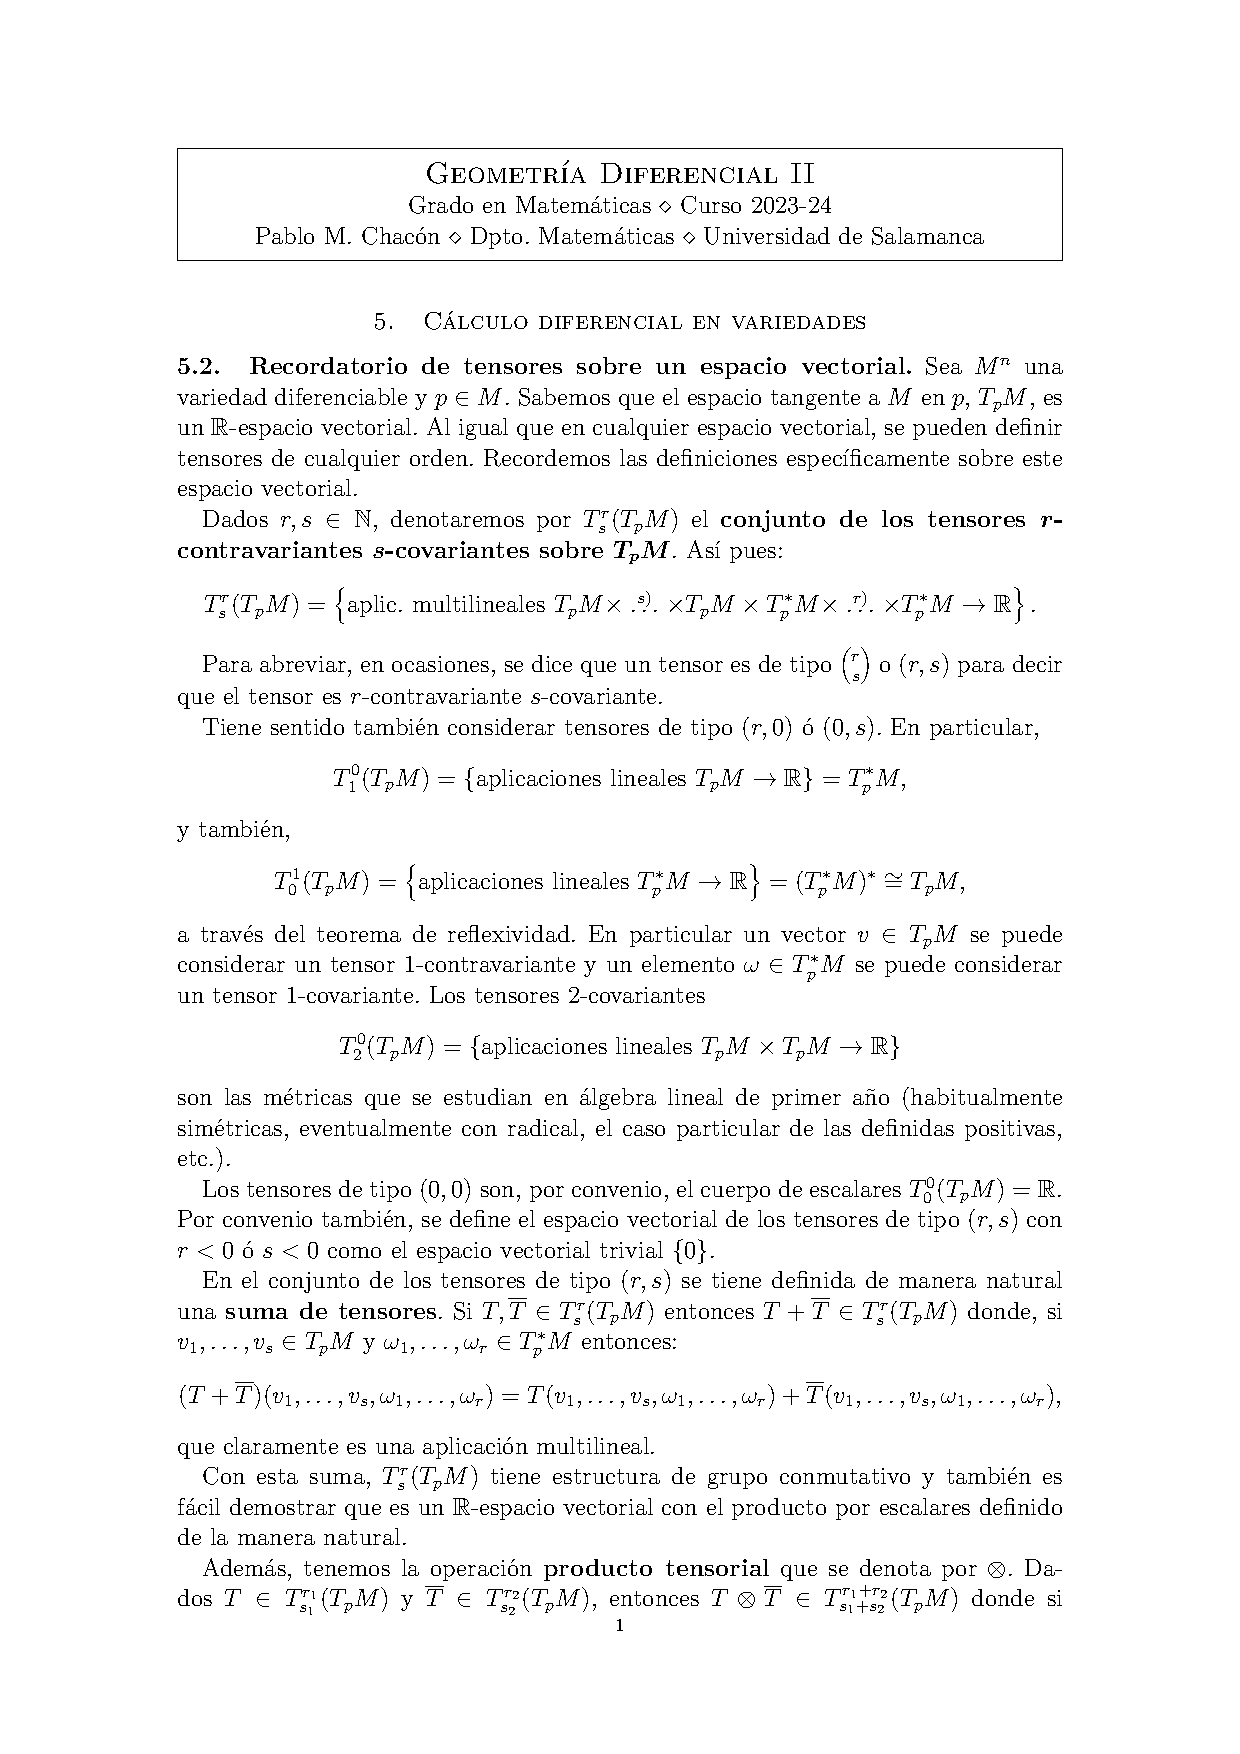
\includepdf[pages={1-9}]{Chapters/Tema5_tensores_espacios_vectoriales.pdf}\label{ap1} 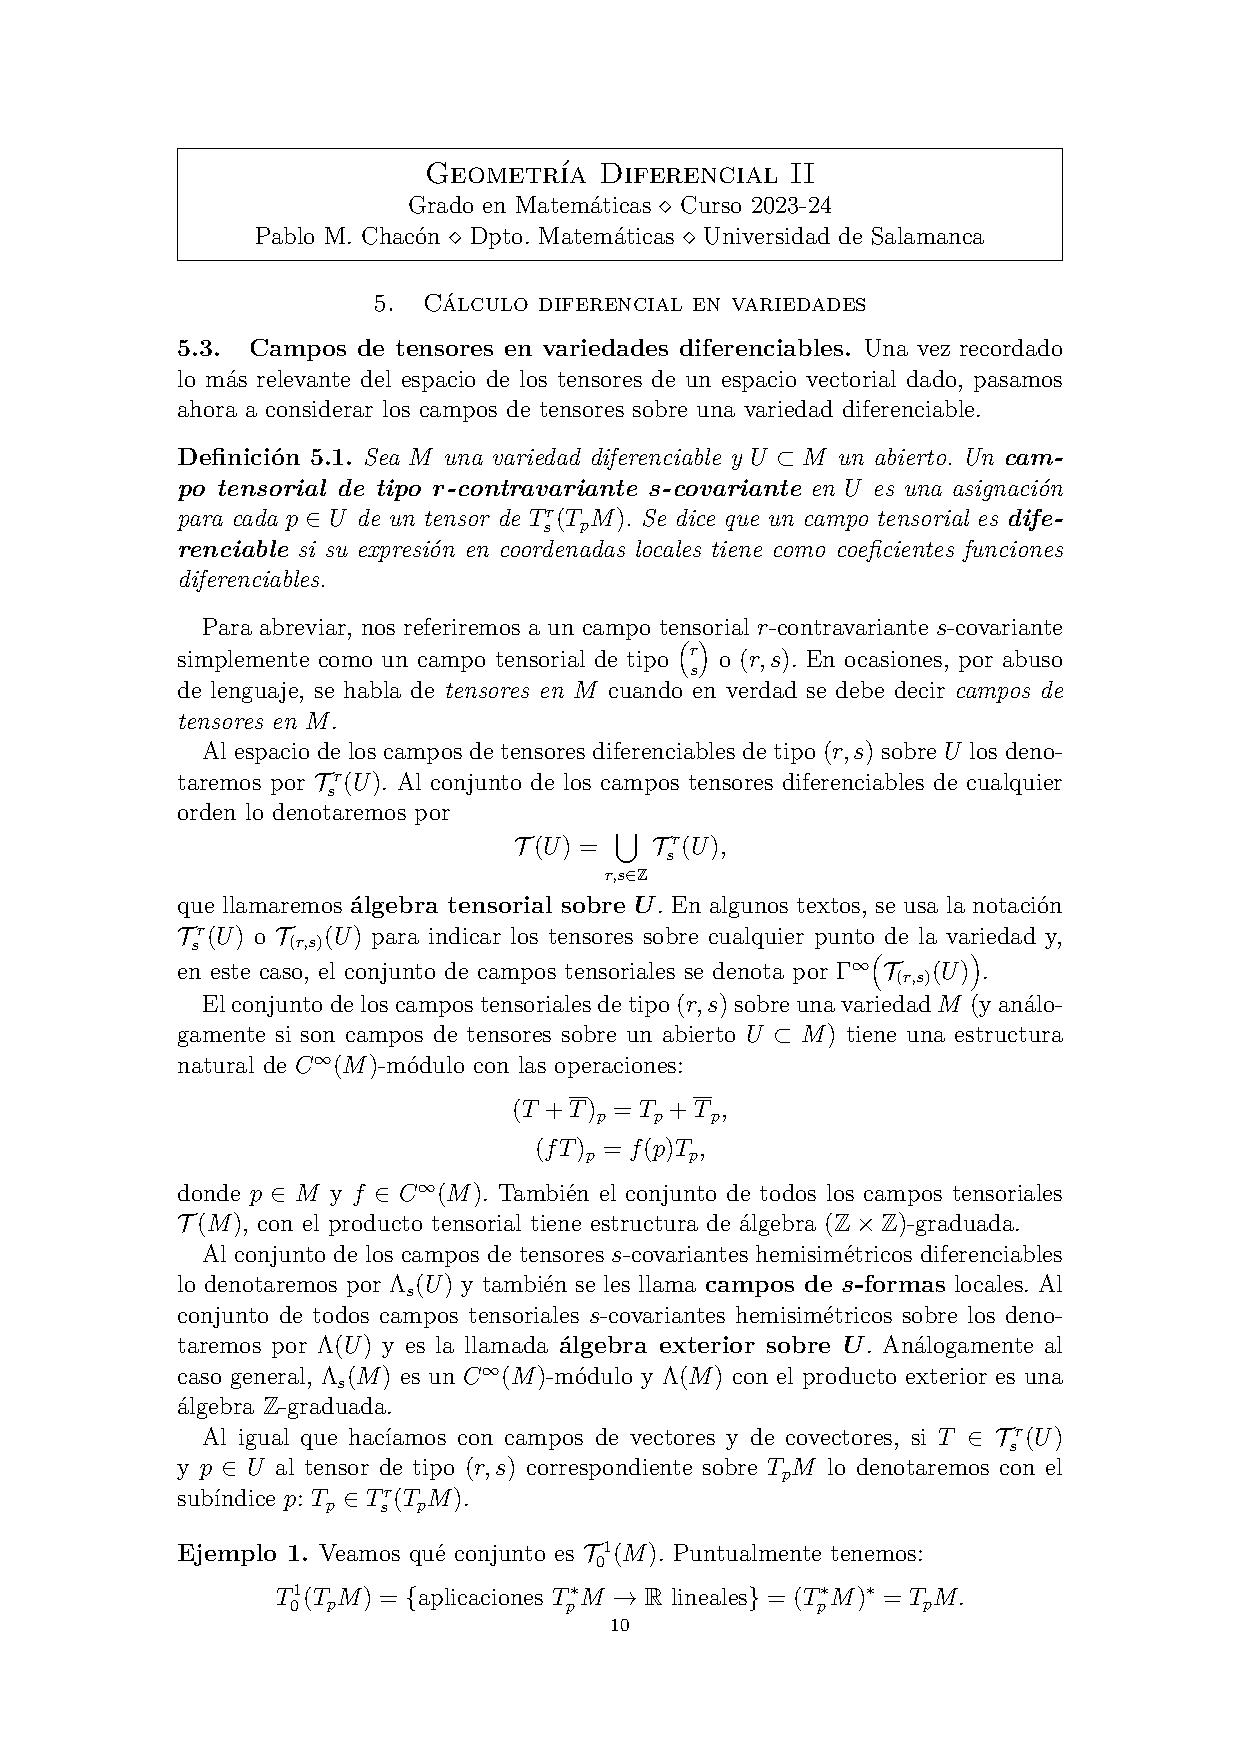
\includepdf[pages={1-7}]{Chapters/Tema5_campos_tensoriales.pdf}\label{ap2} 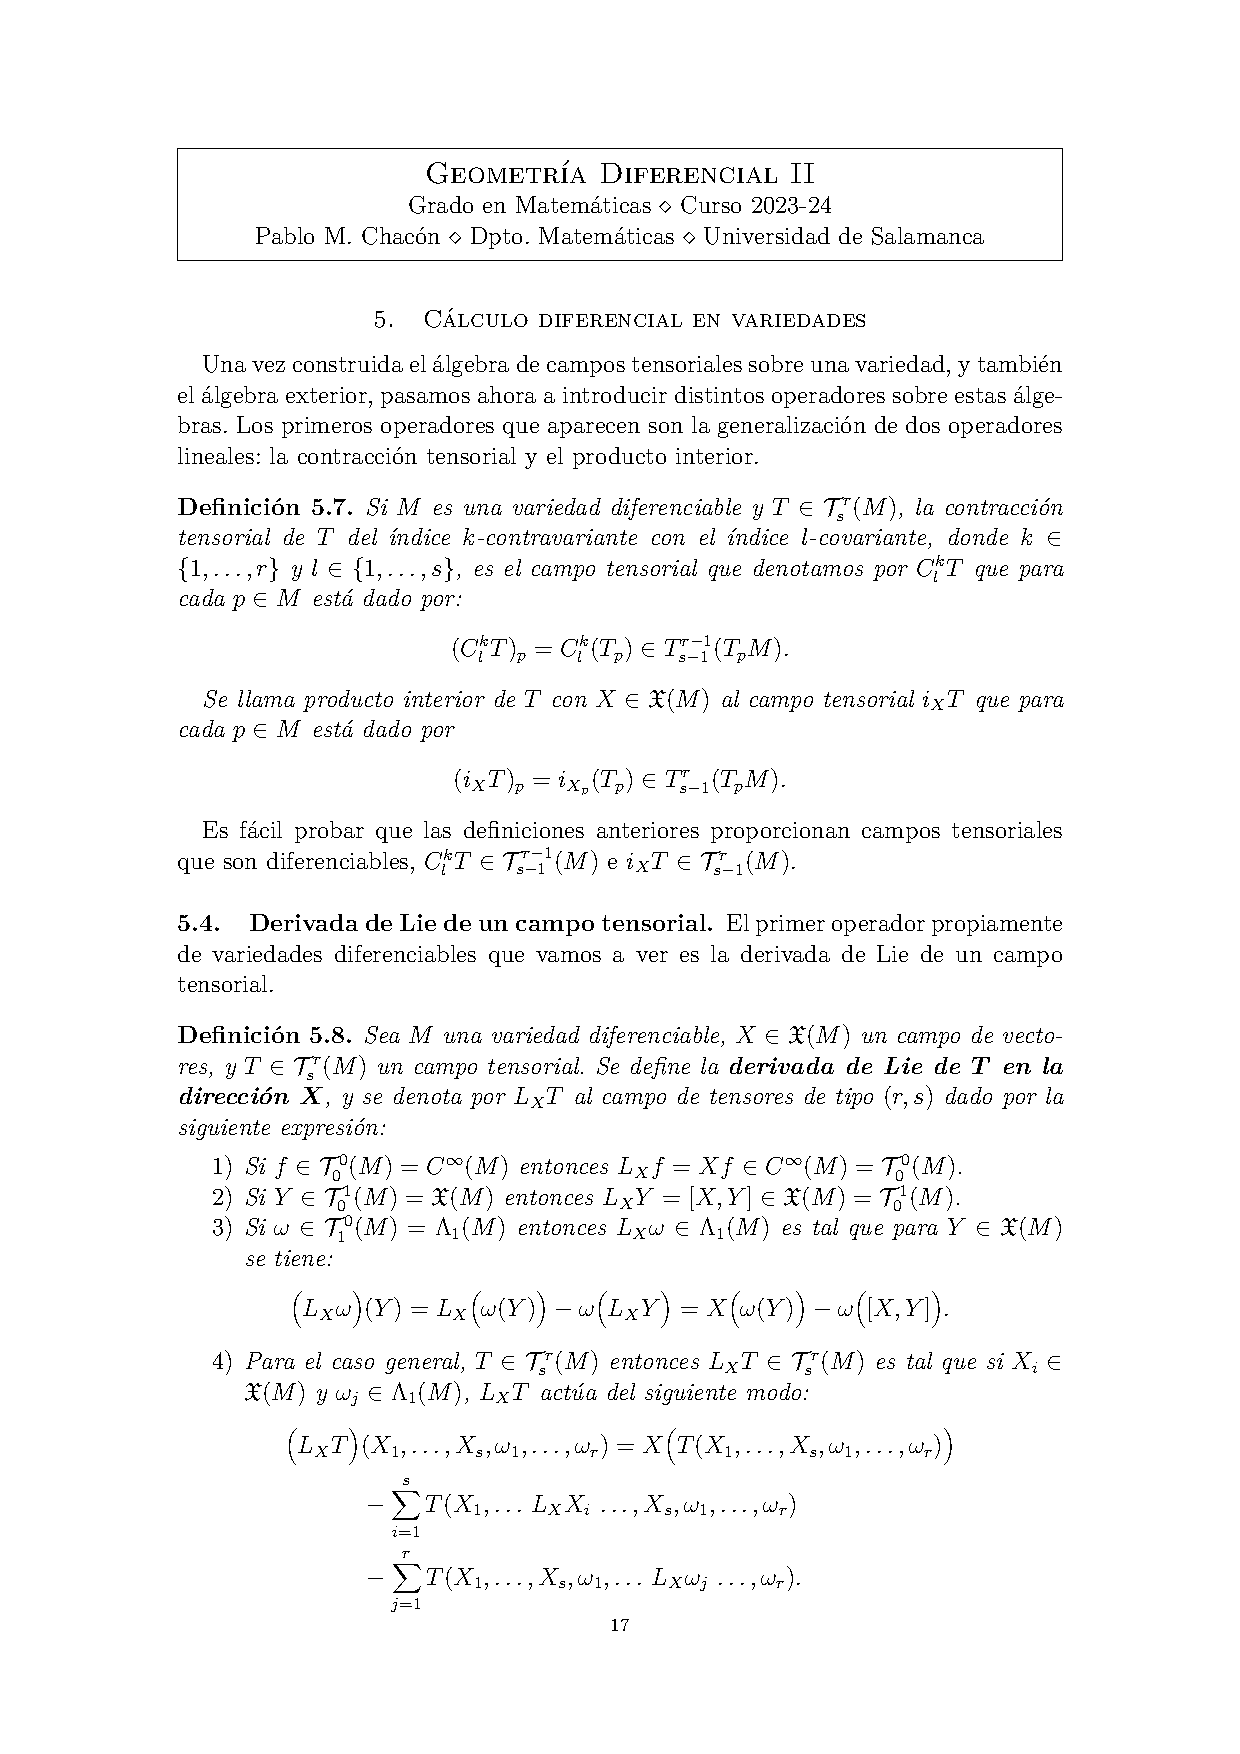
\includepdf[pages={1-11}]{Chapters/studium_Tema5_derivada_Lie.pdf}\label{ap3} 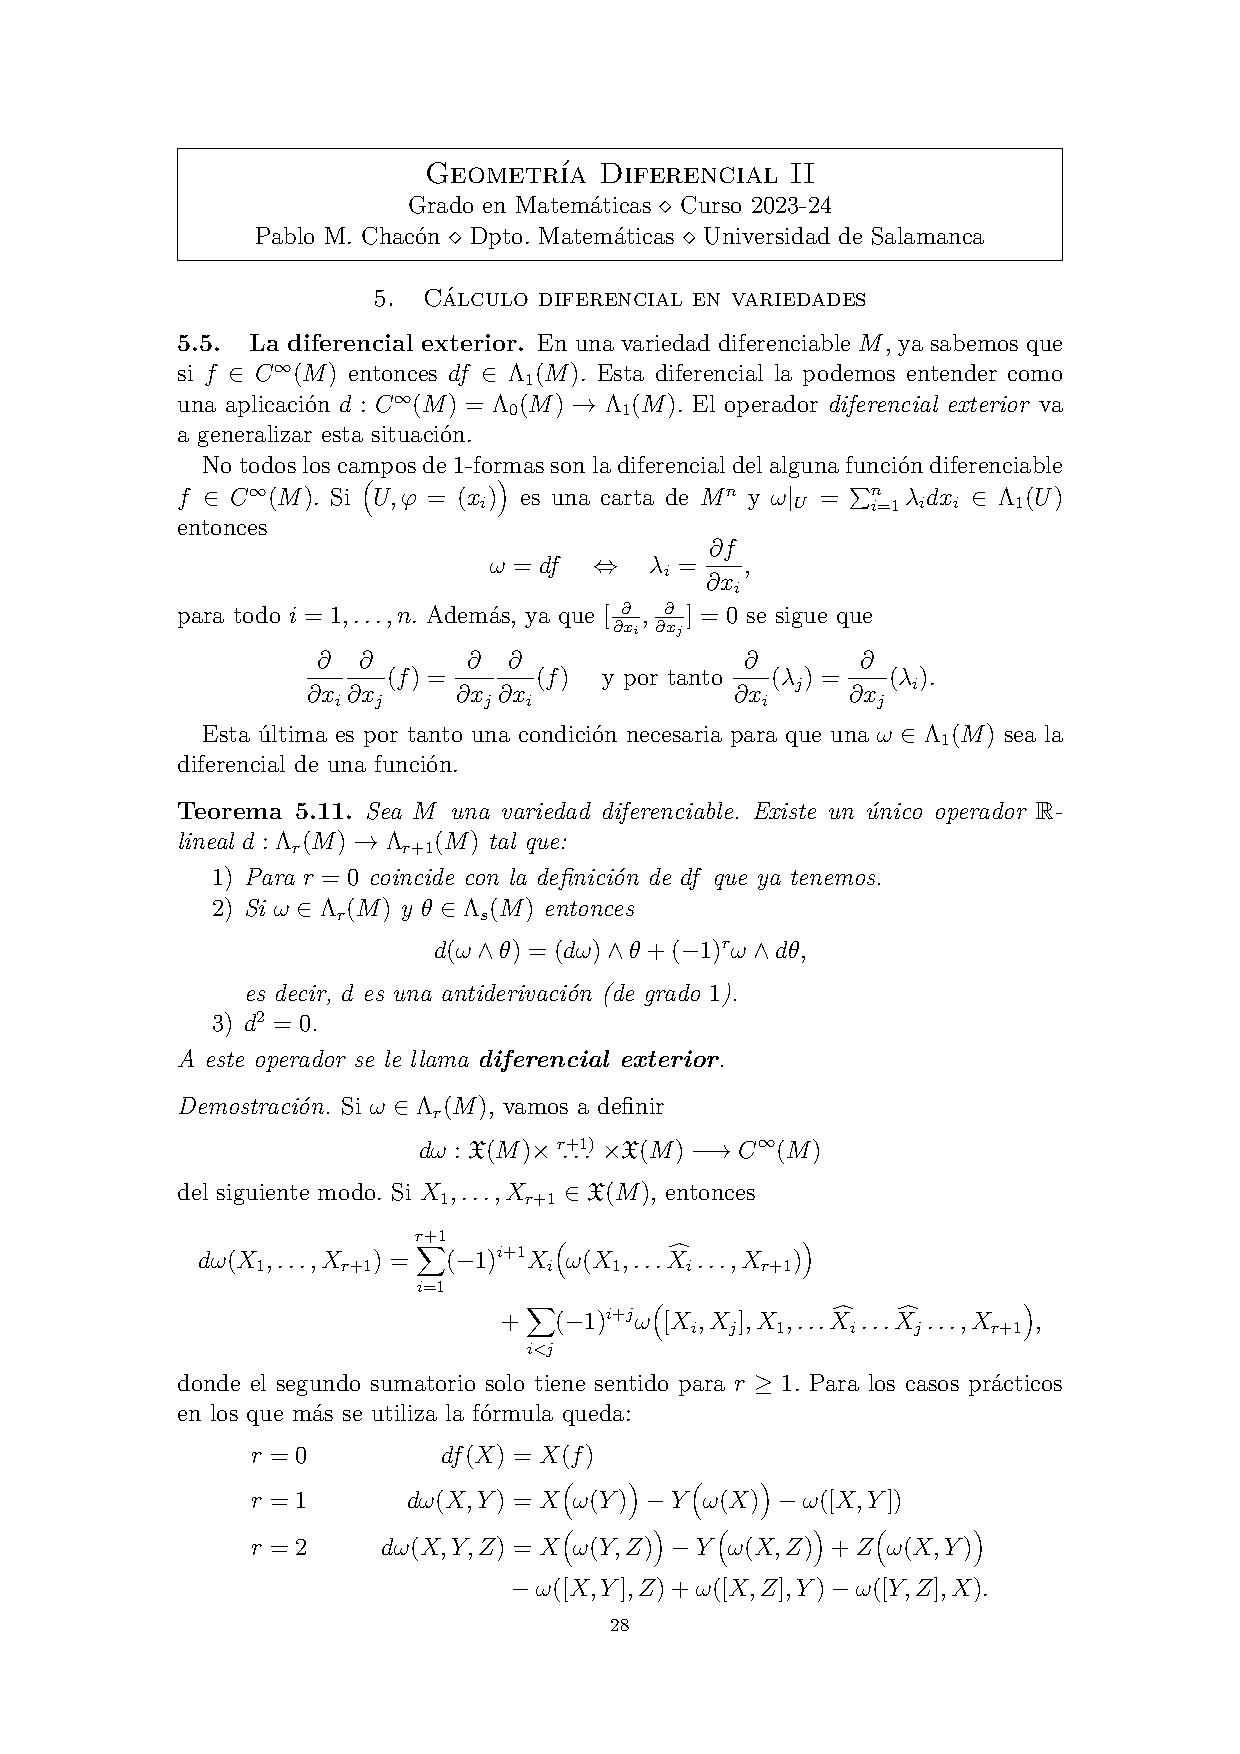
\includepdf[pages={1-13}]{Chapters/studium_Tema5_diferencial_exterior.pdf}\label{ap4}

\standardchapterstyle

\end{document}